\documentclass[11pt,a4paper,twoside,openany]{book}
\usepackage{lifeos}
\usepackage{pgfplots}\pgfplotsset{compat=1.17}
\usetikzlibrary{positioning}
\usepackage{circuitikz}
\usepackage{graphicx}
\usepackage[font=small,labelfont=bf]{caption}
\usepackage{subcaption}
\usepackage{makeidx}\makeindex
\setlifeostitle{Competitive Programming and Algorithms}
\setcounter{tocdepth}{1}

\begin{document}
\frontmatter
\pagestyle{empty}
\makecover{Competitive Programming and Algorithms}{From first submission to gold}{Study textbook}
\newpage\pagestyle{fancy}
\tableofcontents
\mainmatter
\chapter{The contest machine and the cost model}\label{ch:machine}
\index{contest workflow}

Competitive programming is a game played inside a strict machine: a judge
compiles your program, runs it on hidden tests, and returns a one-word verdict
in seconds. This chapter teaches you how that machine works and how to think
inside it. By the end you will have a starter file you trust, a working sense
of how fast a given algorithm is before you write it, and a routine for going
from a problem statement to an accepted submission without flailing. Everything
else in the book assumes this chapter's machinery.

\section{How a judge sees your program}\label{sec:judge}

Forget the IDE, the debugger, the terminal prompt. To the judge\index{judge}
your program is a \emph{function}: it reads characters from standard input
(\texttt{stdin}\index{stdin}) and writes characters to standard output
(\texttt{stdout}\index{stdout}). No files, no network, no graphics, no prompts.
A program that prints \texttt{please enter n:} gets marked wrong, because the
judge compares your output byte-for-byte with the expected output.

A submission is run once per \emph{test file}. Each test file is one complete
input; your program must print the correct answer for it within the
\emph{time limit}\index{time limit} (typically 1--2 seconds) and the
\emph{memory limit}\index{memory limit} (typically 256--512\,MB). The tests are
hidden from you. They are also written by people whose job is to break
plausible-but-wrong programs, so ``it worked on my three tests'' means nothing.

After all runs, the judge reports one \emph{verdict}\index{verdict} per
submission, sometimes per test:

\begin{center}
\begin{tabular}{ll}
\toprule
\thead{Verdict} & \thead{Meaning}\\
\midrule
Accepted (AC) & every test file passed\\
Wrong Answer (WA) & your output differed from the expected output\\
Time Limit Exceeded (TLE) & a run did not finish inside the time limit\\
Runtime Error (RE) & the program crashed (segfault, bad index, \dots)\\
Memory Limit Exceeded (MLE) & the program exceeded the memory budget\\
Compile Error (CE) & the judge could not build your code\\
\bottomrule
\end{tabular}
\end{center}

Figure~\ref{fig:verdict} shows the whole pipeline; Figure~\ref{fig:statement}
annotates a typical statement so you can see where the machine's parameters
are declared.

\begin{figure}[ht]\centering
% fig01-verdict.tex -- Figure 1.1: what the judge does with a submission.
\begin{tikzpicture}[
  font=\small,
  box/.style={draw, rounded corners=1.5pt, minimum height=7.5mm,
              inner xsep=6pt, fill=graybg},
  good/.style={draw, rounded corners=1.5pt, minimum height=6.5mm,
              inner xsep=5pt, fill=goodbg},
  bad/.style={draw, rounded corners=1.5pt, minimum height=6.5mm,
              inner xsep=5pt, fill=amberbg},
  lab/.style={font=\footnotesize, text=slate},
  arr/.style={-{stealth}, thick}
]
\node[box] (sub) at (0,0) {source code};
\node[box, right=7mm of sub] (comp) {compile};
\node[box, right=7mm of comp] (run) {run on hidden tests};
\node[good, right=7mm of run, yshift=9mm] (ac) {Accepted};
\node[bad,  right=7mm of run, yshift=-9mm] (rej) {Rejected};
\draw[arr] (sub) -- (comp);
\draw[arr] (comp) -- (run);
\draw[arr] (run) -- (ac) node[midway, above, lab] {every test passed};
\draw[arr] (run) -- (rej) node[midway, below, lab] {any failure};
\draw[arr] (comp.south) |- ($(comp.south)+(0,-5mm)$) -|
  node[lab, pos=0.75, left] {does not compile} (rej.north);
\node[lab, text width=12.4cm, align=center] at ($(run.south)+(0.4,-1.9)$)
  {Rejected comes in five flavours: \textbf{WA} wrong answer,
   \textbf{TLE} too slow, \textbf{RE} crash, \textbf{MLE} too much memory,
   \textbf{CE} never built};
\end{tikzpicture}

\caption{What the judge does with your code. Notice there is only one good
outcome and five distinct ways to lose; each failure tells you where to look
first. CE means the file did not build at all --- fix that before anything
else.}
\label{fig:verdict}
\end{figure}

\begin{figure}[ht]\centering
% fig02-statement.tex -- Figure 1.2: anatomy of a problem statement.
% The statement itself is invented for this book; the layout follows
% the CSES / USACO convention of name, limits, task, I/O, example.
\begin{tikzpicture}[font=\small]
\node[draw=ink, fill=white, text width=7.8cm, inner sep=8pt, font=\footnotesize,
      align=flush left, anchor=north west] (stmt) at (0,0) {%
  {\sansfont\bfseries Apple Sums}\quad{\color{slate}time 1.0 s \quad memory 256 MB}\\[4pt]
  \textbf{Task.} A shop sells $n$ kinds of apples. Kind $i$ costs $a_i$ rupiah.
  Find the cheapest way to buy exactly $k$ apples (any kinds, repeats allowed),
  or report $-1$ if impossible.\\[4pt]
  \textbf{Input.} First line: $n$ and $k$. Second line: $a_1,\dots,a_n$.\\[4pt]
  \textbf{Output.} One integer: the minimum total cost, or $-1$.\\[4pt]
  \textbf{Constraints.} $1 \le n \le 10^5$, $1 \le k \le 10^9$,
  $1 \le a_i \le 10^9$.\\[4pt]
  \textbf{Example.} Input \texttt{3 5 / 4 2 9} $\to$ output \texttt{10}.};
\begin{scope}[font=\footnotesize, text=accent, text width=3.7cm, align=flush left, anchor=west]
\node (c1) at (8.9,-0.45) {\textbf{limits:} the budget your program lives under};
\node (c2) at (8.9,-1.75) {\textbf{I/O contract:} what stdin gives, what stdout must print};
\node (c3) at (8.9,-3.05) {\textbf{constraints:} these numbers choose the algorithm};
\node (c4) at (8.9,-4.2) {\textbf{example:} a handshake test, not a proof};
\end{scope}
\draw[-{stealth}, accent, thick] (c1.west) -- (8.35,-0.45);
\draw[-{stealth}, accent, thick] (c2.west) -- (8.35,-1.45);
\draw[-{stealth}, accent, thick] (c3.west) -- (8.35,-2.5);
\draw[-{stealth}, accent, thick] (c4.west) -- (8.35,-3.2);
\end{tikzpicture}

\caption{Anatomy of a problem statement (invented here, in the layout CSES and
USACO use). Notice the constraints block: it is the most important paragraph
on the page, and Section~\ref{sec:constraints} teaches you to read it before
reading anything else.}
\label{fig:statement}
\end{figure}

Scoring varies by contest. CSES and most archives are all-or-nothing: a
submission is worth points only if every test passes. USACO gives partial
credit per test file. IOI-style problems and some Codeforces subtasks give
partial credit for easier constraint ranges --- you can AC the small
\emph{subtasks}\index{subtask} while the hard ones stay red. Always read which
model a problem uses; it changes which submissions are worth your time.

\begin{exercise}[easy]\label{exr:verdicts}
A friend submits three programs to the same problem. Predict each verdict:
(a) the program prints \texttt{answer: 42} instead of \texttt{42};
(b) the program is correct but takes 30 seconds on the largest test;
(c) the program declares \texttt{int a[1000000000];} inside \texttt{main}
(a four-gigabyte stack array).
\end{exercise}

\begin{example}[WE 1.1 --- CSES \emph{Weird Algorithm}: the full loop]
\label{ex:weird}
A problem asks: given an integer $n$ up to $10^6$, print the sequence where
each step halves an even number and sends an odd number to $3n+1$, ending at
$1$. Input \texttt{3} should print \texttt{3 10 5 16 8 4 2 1}.
\par\smallskip
\textbf{Strategy.} There is nothing to optimise: the statement \emph{is} the
algorithm, so simulate it directly. The only question is the integer type ---
intermediate values can exceed $10^6$ even when the input does not. (For the
record: starting from $n=704\,511$, legal under the limit, the sequence peaks
at $56\,991\,483\,520$.) A 32-bit \texttt{int} would overflow on a fraction of
tests, so use 64 bits.
\par\smallskip
\begin{solution}
\begin{lstlisting}
#include <iostream>
using namespace std;
using ll = long long;
int main() {
    ll n;
    cin >> n;
    while (n != 1) {
        cout << n << ' ';
        n = (n % 2 == 0) ? n / 2 : 3 * n + 1;
    }
    cout << 1 << '\n';
}
\end{lstlisting}
Run on the sample:
\begin{lstlisting}[numbers=none]
$ echo 3 | ./weird
3 10 5 16 8 4 2 1
\end{lstlisting}
It matches, so we also check the edge case $n=1$ (prints \texttt{1}
immediately) before submitting. The submission returns AC. The real workflow
here is what matters: read, simulate, test on the sample, test one edge case,
submit. You will repeat it hundreds of times.
\end{solution}
\end{example}

\section{The C++17 starter kit}\label{sec:starter}
\index{starter file|see{template}}
\index{template}

Every solution in this book is C++17. Listing~\ref{lst:template} is the
starter file; it lives in \texttt{code/lib/} and every later chapter
copies it.

\lstinputlisting[caption={\texttt{code/lib/template.cpp}: the starter file.
Minimal on purpose --- every line earns its place.},label={lst:template}]
{code/lib/template.cpp}

Three choices in it deserve a defence. First, the includes are explicit.
You will see \texttt{\#include <bits/stdc++.h>} in other people's code; judges
accept it, but it is a GCC-specific catch-all, it hides which facilities you
actually use, and it fails on compilers that do not ship it. We name the four
headers this chapter needs and add others as the book demands them.

Second, \texttt{using ll = long long}. The default integer type for counting
should be 64-bit: \texttt{int}\index{int@{\texttt{int}}} holds only
about $\pm 2.1\cdot 10^9$, while \texttt{ll} holds about
$\pm 9.2\cdot 10^{18}$. The price is a few characters and roughly twice the
memory per number --- cheap insurance against the single most common WA cause
in the archive.

Third, the two macros. \texttt{rep(i,a,b)} is a counted loop;
\texttt{all(x)} expands to \texttt{begin(x), end(x)} for calls like
\texttt{sort(all(v))}. We keep the macro count at two because macros are
invisible at read time --- a template that does magic for you will do magic
\emph{to} you in a later chapter's debugging session.

\begin{definition}[Integer overflow]\index{overflow}
\emph{Overflow} is arithmetic leaving the range of its type. In C++ signed
overflow is \emph{undefined behaviour}\index{undefined behaviour}: the standard
allows anything. In practice the value usually wraps to garbage
($2\,147\,483\,647+1$ becomes $-2\,147\,483\,648$), but ``usually'' is the
point --- the same code can misbehave differently across compilers and flags.
\end{definition}

The rules of thumb: any product of two inputs near $10^5$ or larger, any sum
of up to $10^5$ terms near $10^9$, and any expression like \texttt{n*(n+1)/2}
with $n$ above $46\,000$ exceeds \texttt{int}. When in doubt, \texttt{ll}.

\begin{tripwire}[The overflow tripwire]
If a program passes the samples but fails the judge's big tests, check the
types of every accumulator and every product \emph{before} anything else.
Worked Example 1.4 is this exact failure.
\end{tripwire}

\subsection{Fast input and output}\label{sec:fastio}
\index{fast input/output}
\index{ios::sync\_with\_stdio@\texttt{ios::sync\_with\_stdio}}

By default, C++ streams are synchronised with the C stdio library --- a
convenience you pay for on every \texttt{cin}. Two lines in the template turn
that off: \texttt{ios::sync\_with\_stdio(false)} detaches the streams, and
\texttt{cin.tie(nullptr)} stops \texttt{cin} from flushing \texttt{cout}
before each read. Together they make stream I/O fast enough for almost every
problem in this book.

When input gets large --- a million tokens or more --- even that can be the
bottleneck. Listing~\ref{lst:fastscan} compares the two levels on a file of
one million integers: plain \texttt{cin} with sync disabled versus a small
scanner that reads the raw \texttt{stdin} buffer itself
(\texttt{code/lib/fastscan.h}, part of the capstone library).

\lstinputlisting[caption={\texttt{code/fastscan.cpp}: two ways to read a
million integers, timed.},label={lst:fastscan}]{code/fastscan.cpp}

\begin{checkpoint}[Predict before you run]
Predict the ratio of the two timings: a factor of 2, of 10, or of 100? Then
look at the measured run below.
\end{checkpoint}

\begin{lstlisting}[numbers=none]
$ ./fastscan < ints1e6.txt
method=cin sum=499884612927859 time_ms=919.0
$ ./fastscan f < ints1e6.txt
method=fread sum=499884612927859 time_ms=6.6
\end{lstlisting}

On this machine the buffer scanner is about $140\times$ faster --- nine
hundred milliseconds spent purely on parsing. Take the lesson as a range, not
a law: the ratio varies by machine and judge, but the direction never does.
Use the template's two lines always; reach for \texttt{fastscan.h} when input
is the bottleneck.

\subsection{The STL you actually use}\label{sec:stl}
\index{STL}\index{vector@\texttt{vector}}\index{sort@\texttt{sort}}

You can solve the first hundred problems of this book with five library
tools. \texttt{vector} is the only array you need: contiguous, resizable,
O(1) index access. \texttt{sort} orders a range in $O(n\log_2 n)$ and accepts
a \emph{comparator}\index{comparator} --- a function returning true when the
first argument belongs before the second. \texttt{set}\index{set@\texttt{set}}
keeps distinct elements sorted (insert, erase, find all $O(\log_2 n)$);
\texttt{map}\index{map@\texttt{map}} is the same idea keyed by a value, which
makes it a frequency table; \texttt{priority\_queue}\index{priority queue}
keeps the current maximum on top in $O(\log_2 n)$ per operation. Strings are
\texttt{std::string}; small records are \texttt{pair} or \texttt{tuple},
unpacked by a \emph{structured binding}\index{structured binding}
(\texttt{auto\& [k, v] : m}). Listing~\ref{lst:stltour} exercises all of them.

\lstinputlisting[caption={\texttt{code/stl\_tour.cpp}: the four containers
and a custom comparator, with real output.},label={lst:stltour}]
{code/stl_tour.cpp}

\begin{lstlisting}[numbers=none]
sorted: 2 4 8 1 5
set: 1 2 4
a=2 b=3 c=1 
pop order: 9 7 4 3
\end{lstlisting}

Notice the comparator's effect on the first line: evens sorted before odds,
each group ascending. Notice too that \texttt{freq[w]++} needs no
initialisation --- \texttt{map} value-initialises missing entries to zero,
which is why frequency tables are one line of code.

\begin{exercise}[easy]\label{exr:predict}
Predict the output of this program, then check yourself by running it:
\begin{lstlisting}
int a = 7;
cout << a/2 << ' ' << a/2.0 << ' ' << (a*a)/2 << '\n';
\end{lstlisting}
What type does the middle expression evaluate in, and why do the first and
last answers differ?
\end{exercise}

\section{Time complexity}\label{sec:complexity}
\index{time complexity}

``Is this algorithm fast enough?'' has to be answerable \emph{before} you
write code, or you will spend contest minutes implementing something that was
doomed from the statement. The tool is asymptotic analysis: count how the
work grows with the input size, not how many milliseconds it takes on one
machine.

\begin{definition}[RAM model]\index{RAM model}
We count \emph{operations}: arithmetic, comparisons, assignments, array
reads and writes each cost one unit. A function call is the sum of the work
it does. This is a model, not physics --- real machines have caches,
branches and vector units --- but it predicts the shape of runtimes far
better than it predicts their absolute values.
\end{definition}

Count the operations in a nested loop exactly once and you will see why the
abstraction helps:

\begin{lstlisting}
long long s = 0;                       // 1 op
for (int i = 0; i < n; ++i)            // n iterations
    for (int j = i + 1; j < n; ++j)    // n-i-1 iterations
        s += a[i] * a[j];              // 3 ops each pass
\end{lstlisting}

The innermost line runs $\sum_{i=0}^{n-1}(n-1-i) = n(n-1)/2$ times, so the
total is $1 + 3n(n-1)/2$. For large $n$ the $n^2$ term dominates: at
$n=10^5$ the count is about $1.5\cdot 10^{10}$ --- seconds to minutes, not
the microseconds a linear algorithm needs. The lower-order terms and the
constants stop mattering quickly, which is exactly what the notation
formalises.

\begin{definition}[$O$, $\Theta$, $\Omega$]\index{big-O}\index{Theta@$\Theta$}%
\index{Omega@$\Omega$}
For functions $f,g:\mathbb{N}\to\mathbb{R}_{>0}$:
\begin{itemize}
\item $f \in O(g)$: there exist $c>0$ and $n_0$ with
$f(n) \le c\,g(n)$ for all $n\ge n_0$ --- $g$ is an \emph{asymptotic upper
bound}.
\item $f \in \Omega(g)$: there exist $c>0$ and $n_0$ with
$f(n) \ge c\,g(n)$ for all $n\ge n_0$ --- an asymptotic lower bound.
\item $f \in \Theta(g)$: both hold --- $f$ and $g$ have the same growth rate.
\end{itemize}
Writing $f = O(g)$ is common shorthand for $f \in O(g)$.
\end{definition}

\begin{theorem}\label{thm:thetapoly}
$3n^2 + 10n + 7 \in \Theta(n^2)$.
\end{theorem}

\begin{proof}
Upper bound: for $n \ge 1$, $10n \le 10n^2$ and $7 \le 7n^2$, so
$3n^2+10n+7 \le 20n^2$; take $c=20$, $n_0=1$ and $f \in O(n^2)$.
Lower bound: for $n \ge 1$, $3n^2+10n+7 \ge 3n^2$; take $c=3$, $n_0=1$
and $f \in \Omega(n^2)$. Both directions hold, so $f \in \Theta(n^2)$.
\end{proof}

The same squeeze works for any polynomial: the leading term is the whole
story. Inside $O(\cdot)$ the base of a logarithm never matters either, since
$\log_a n = \log_b n / \log_b a$ differs only by a constant; in this book
complexity uses $\log_2$ to keep the concrete meaning --- the number of
halvings --- and every other $\log$ is natural.

The classes that matter, from cheapest to most expensive:

\begin{center}
\begin{tabularx}{\linewidth}{@{}lYY@{}}
\toprule
\thead{Class} & \thead{Name} & \thead{Produced by}\\
\midrule
$O(1)$ & constant & a formula, one array lookup\\
$O(\log_2 n)$ & logarithmic & halving the input each step (binary search)\\
$O(\sqrt{n})$ & square root & per-block passes in sqrt decomposition\\
$O(n)$ & linear & one pass over the input\\
$O(n\log_2 n)$ & log-linear & sorting; divide and conquer without blowup\\
$O(n^2)$ & quadratic & all pairs; doubly nested loops\\
$O(n^3)$ & cubic & all triples; some DP on small $n$\\
$O(2^n)$ & exponential & enumerating all subsets\\
$O(n!)$ & factorial & enumerating all permutations\\
\bottomrule
\end{tabularx}
\end{center}

\begin{figure}[ht]\centering
% fig03-growth.tex — Figure 1.3: operation-count growth vs the 1 s budget.
% Log-log axes; the 1e8-op line marks one second of simple work.
\begin{tikzpicture}
\begin{loglogaxis}[
    width=0.86\linewidth, height=6.8cm,
    xlabel={input size $n$}, ylabel={operations},
    xmin=1, xmax=1e8, ymin=1, ymax=1e17,
    legend pos=south east, legend style={font=\footnotesize},
    grid=major, grid style={gray!22},
    tick label style={font=\footnotesize},
    label style={font=\small}]
\addplot[domain=1:1e8, samples=60, thick, accent] {ln(x)/ln(2)};
\addplot[domain=1:1e8, samples=60, thick] {x};
\addplot[domain=1:1e8, samples=80, thick, dashed] {x*ln(x)/ln(2)};
\addplot[domain=1:1e8, samples=60, thick, dotted] {x^2};
\addplot[domain=1:60,   samples=61, thick, dashdotted] {2^x};
\addplot[domain=1:1e8, samples=2, thin, amber] {1e8};
\legend{$\log_2 n$, $n$, $n\log_2 n$, $n^2$, $2^n$, 1-second budget ($10^8$)}
\end{loglogaxis}
\end{tikzpicture}

\caption{Operation counts on log--log axes against the one-second budget of
$10^8$ simple operations. Notice where each curve crosses the amber line:
$\log_2 n$ never gets there, $n\log_2 n$ crosses near $n \approx 4\cdot10^6$,
$n^2$ near $10^4$, and $2^n$ already fails before $n=30$. This single picture
is the whole point of Section~\ref{sec:constraints}.}
\label{fig:growth}
\end{figure}

\begin{definition}[The $10^8$ heuristic]\index{10^8 heuristic@$10^8$ heuristic}
As a budgeting rule of thumb, one second of judge time buys roughly $10^8$
\emph{simple} operations --- integer adds, compares, array touches. It is a
heuristic, not a law: memory-bound passes can be slower, vectorised inner
loops can be several times faster, and the number says nothing about a
two-second or ten-second limit. Use it to compare candidate algorithms, not
to certify one.
\end{definition}

\begin{exercise}[medium]\label{exr:countops}
Count the operations in this fragment exactly, then give its $\Theta$-class:
\begin{lstlisting}
for (int i = 1; i <= n; ++i)
    for (int j = 1; j <= i; j += 2)
        work();
\end{lstlisting}
Hint: the inner trip count is $\lceil i/2 \rceil$.
\end{exercise}

\section{From constraints to a plan}\label{sec:constraints}
\index{constraints}

Statements hand you the input size $n$ on a plate. The contest skill is
converting $n$ into the \emph{largest} complexity class that survives the
budget --- Figure~\ref{fig:constraints} is the table every experienced
contestant has internalised --- and then picking the simplest algorithm in
that class.

\begin{figure}[ht]\centering
% fig04-constraints.tex -- Figure 1.4: the constraint-to-complexity table,
% drawn as a boxed chart (a figure, not body text).
\renewcommand{\arraystretch}{1.25}%
\begin{tabular}{@{}r l l@{}}
\toprule
\thead{largest $n$} & \thead{needs at most} & \thead{typical shapes}\\
\midrule
$n \le 12$      & $O(n!)$                 & permutations, brute force\\
$n \le 25$      & $O(2^n)$                & subsets, meet-in-the-middle\\
$n \le 500$     & $O(n^3)$                & all triples, $n\times n$ DP\\
$n \le 5\,000$  & $O(n^2)$                & all pairs, quadratic DP\\
$n \le 2\cdot 10^5$ & $O(n\log_2 n)$    & sorting, sets, Fenwick\\
$n \le 10^7$    & $O(n)$                  & single linear pass\\
any $n$         & $O(\log_2 n)$ or $O(1)$ & binary search, closed formula\\
\bottomrule
\end{tabular}%
\\[4pt]
\begin{minipage}{0.9\linewidth}\footnotesize\color{slate}
Assumes the $10^8$-ops-per-second budget. Rows are rules of thumb, not laws:
a $5\cdot 10^7$-constant quadratic can still lose to a linear algorithm.
\end{minipage}

\caption{The constraint-to-complexity table. Notice it is a ceiling chart:
$n\le 2\cdot10^5$ does not demand $O(n\log_2 n)$, it \emph{forbids} anything
slower. Rows are rules of thumb under the $10^8$ heuristic; a
$5\cdot10^7$-constant quadratic can still lose to a linear pass.}
\label{fig:constraints}
\end{figure}

Two refinements before the table gets used. First, judge tests are built to
stress the \emph{worst case}\index{worst case}: average-case reasoning is how
quicksort dies on sorted input. Plan for the worst row in Figure's table,
not the typical one. Second, \emph{constant factors}\index{constant factor}
are real --- an $O(n\log_2 n)$ algorithm whose inner step rebuilds a
\texttt{set} can lose to a well-written $O(n)$ pass at the same $n$ --- but
constants lose to growth: no constant rescues $n^2$ when $n=10^6$.

\begin{rulebox}[Choosing the algorithm]
Let $C$ be the largest class that fits the constraint table for the given
$n$. Among algorithms in $C$, implement the \emph{simplest correct one you
can explain} --- the one with the fewest moving parts. If it TLEs, only then
reach for the cleverer algorithm in the same class. Never climb the table
first: a fancy $O(n\log_2 n)$ where $O(n^2)$ would have passed is wasted
minutes.
\end{rulebox}

\begin{example}[WE 1.2 --- CSES \emph{Maximum Subarray Sum}, four ways]
\label{ex:mss}
Given an array of $n$ integers (with negatives), find the largest sum of a
contiguous subarray. On CSES, $n \le 2\cdot10^5$: the table says
$O(n\log_2 n)$ or better.
\par\smallskip
\textbf{Strategy.} Same problem, four honest attempts, each removing one
structural waste: (i) try every interval and resum --- correct but cubic;
(ii) keep the sum running while the right end moves --- quadratic;
(iii) split the array and combine --- $O(n\log_2 n)$;
(iv) notice that only the \emph{best ending} matters at each step ---
linear.
\par\smallskip
\begin{solution}
The cubic version checks all $n(n+1)/2$ intervals and resums each:
\begin{lstlisting}
for (int l = 0; l < n; ++l)
    for (int r = l; r < n; ++r) {
        ll s = 0;
        for (int k = l; k <= r; ++k) s += a[k];
        best = max(best, s);
    }
\end{lstlisting}
It is correct --- it inspects every candidate --- and it is the first
submission most beginners write. The quadratic version keeps $s$ running as
$r$ advances, deleting the inner loop. The divide-and-conquer version splits
at the middle: the answer is the best of left half, right half, or an
interval crossing the middle (extend left and right greedily from the
split). The linear version is Kadane's\index{Kadane's algorithm}:
\begin{lstlisting}
ll best = a[0], cur = a[0];
for (int i = 1; i < n; ++i) {
    cur = max(a[i], cur + a[i]);   // extend or restart
    best = max(best, cur);
}
\end{lstlisting}
Correctness, in one line: \texttt{cur} is the largest sum of any subarray
\emph{ending at} $i$ --- you either continue the previous best suffix or
abandon it --- and \texttt{best} remembers the largest of those. All four
are in \texttt{code/mss\_timing.cpp}; Listing~\ref{lst:msstiming} is the
driver. Measured on this machine:
\begin{lstlisting}[numbers=none]
O(n^3)    n=3000    ans=24382 time_ms=254.9
O(n^2)    n=50000   ans=109297 time_ms=602.2
O(nlogn)  n=200000  ans=218662 time_ms=1.8
O(n)      n=200000  ans=218662 time_ms=0.1
O(n)      n=5000000 ans=1565779 time_ms=3.4
\end{lstlisting}
Read the table backwards: the linear pass handles $n=5\cdot10^6$ in less
time than the cubic one needs for $n=3000$ --- and note the \texttt{ans}
column is identical wherever both finished, which is the definition of a
correct optimisation.
\end{solution}
\end{example}

\lstinputlisting[caption={Listing 1.4: the benchmark driver
(\texttt{code/mss\_timing.cpp}, excerpt). Each algorithm is timed at the
largest $n$ it survives in about a second; the linear one is pushed to
$n=5\cdot10^6$ to show headroom.},
label={lst:msstiming},firstline=63,lastline=85]{code/mss_timing.cpp}

We did not run the cubic version at $n=2\cdot10^5$; extrapolating the
measured scaling, it would take about a day. The quadratic at that $n$ is
roughly ten seconds. Both lose the contest to algorithm choice, not to
coding skill --- which is the lesson.

\begin{exercise}[medium]\label{exr:pickclass}
For each problem, name the largest complexity class the constraint allows
under the $10^8$ heuristic and the shape of an algorithm that fits:
(a) $n \le 15$: count the subsets with a given property;
(b) $n \le 3\cdot10^5$: find the maximum of a sliding window;
(c) $n \le 2000$: longest common subsequence of two strings.
\end{exercise}

\section{The submit loop}\label{sec:submit}
\index{submit loop}
\index{sample test}
\index{Wrong Answer|see{verdict}}

Acceptance is a loop, not an event. Figure~\ref{fig:minute} shows how a
working five minutes splits on one problem; the dashed arrow is the part
beginners get wrong --- a WA sends you back to \emph{thinking}, not to
resubmitting.

\begin{figure}[ht]\centering
% fig05-minute.tex — Figure 1.5: how a working five minutes is spent on
% one problem. The same loop returns in Chapter 18 (contest strategy).
\begin{tikzpicture}[font=\small,
  seg/.style={draw, minimum height=8mm, inner xsep=0pt},
  lab/.style={font=\footnotesize},
  num/.style={font=\footnotesize, text=slate}]
% proportional widths: read 30s think 75s code 100s test 45s submit 50s = 300s
\def\u{0.035} % seconds -> cm
\node[seg, fill=graybg,   minimum width=30*\u cm,  anchor=west] (a) at (0,0) {};
\node[seg, fill=accentsoft, minimum width=75*\u cm, anchor=west] (b) at (a.east) {};
\node[seg, fill=graybg,   minimum width=100*\u cm, anchor=west] (c) at (b.east) {};
\node[seg, fill=accentsoft, minimum width=45*\u cm, anchor=west] (d) at (c.east) {};
\node[seg, fill=goodbg,   minimum width=50*\u cm,  anchor=west] (e) at (d.east) {};
\node[lab] at (a.center) {read};
\node[lab] at (b.center) {think};
\node[lab] at (c.center) {code};
\node[lab] at (d.center) {test};
\node[lab] at (e.center) {submit};
\node[num, below=1pt of a.west, anchor=north west] {0:30};
\node[num, below=1pt of b.center] {1:45};
\node[num, below=1pt of c.center] {3:25};
\node[num, below=1pt of d.center] {4:10};
\node[num, below=1pt of e.east, anchor=north east] {5:00};
\draw[{stealth}-, thick, accent] (c.north) -- ++(0,0.5)
  node[above, font=\footnotesize, text=accent]
  {longest block is still under two minutes --- pick the simple plan};
\draw[-{stealth}, dashed, slate] (e.south east) ++(0,-1.1)
  -| node[pos=0.25, below, font=\footnotesize, text=slate]
  {WA $\to$ back to ``think'', not to ``submit again''} (b.south);
\end{tikzpicture}

\caption{One problem, five minutes. Notice the blocks are small and the
feedback edge goes to ``think'': a wrong answer is new information about
your assumptions, not an invitation to submit again.}
\label{fig:minute}
\end{figure}

The loop, expanded. \emph{Compile like the judge}: the book's flags are
\texttt{-std=c++17 -O2 -Wall -Wextra}; warnings are unheeded verdicts.
\emph{Test locally first}: run the samples, then one edge case you invented
($n=1$, all-equal input, the largest legal $n$ if generation is cheap).
\emph{Read a WA as a clue}, in this order:

\begin{checklist}
\item Did I handle the constraints' endpoints ($n=1$, $n=0$, maximum $n$)?
\item Are all accumulators and products 64-bit? (The overflow tripwire.)
\item Does my output match the format byte-for-byte --- no extra words,
spaces, or missing newline?
\item Did I test anything the statement did not give me, or did I trust
the sample?
\end{checklist}

And keep one thing straight: \textbf{Accepted means passed these tests, not
correct}. Judges write strong test sets, but ``AC'' certifies nothing about
inputs nobody tried. The deep fix --- proving your candidate against a brute
force on random small tests --- is \emph{stress testing}\index{stress test},
and Chapter~18 makes it a habit; \texttt{code/test\_ch01.sh} already runs
200 random rounds of the linear MSS code against the cubic one.

\begin{example}[WE 1.3 --- CSES \emph{Missing Number}: two ways to be right]
\label{ex:missing}
Numbers $1$ to $n$ appear once each except one, which is missing. Given
$n \le 2\cdot10^5$ and the $n-1$ present numbers, find the missing one.
\par\smallskip
\textbf{Strategy.} Two routes present themselves: a \emph{formula} ---
the total should be $n(n+1)/2$, so subtract the given sum --- and a
\emph{marking} pass --- record which values appear and find the gap. Both
are $O(n)$, both fit easily. Under time pressure choose the one with fewer
ways to be wrong: the formula's product can overflow if types slip, while
marking has no arithmetic at all beyond indexing. Marking is the safer
submission; the formula is the faster insight. Knowing both lets you pick.
\par\smallskip
\begin{solution}
Formula (\texttt{code/missing\_math.cpp}) and marking
(\texttt{code/missing\_set.cpp}); on the test of Section~1.5 both print
\texttt{200000} for the crafted $n=2\cdot10^5$ case. The point is not the
answer --- it is that two correct algorithms existed and the choice was a
risk decision, not a knowledge gap.
\end{solution}
\end{example}

\begin{example}[WE 1.4 --- the first bug hunt]
\label{ex:bughunt}
Here is a real Wrong Answer. The sum formula for \emph{Missing Number}
written with \texttt{int} throughout (\texttt{code/missing\_int.cpp}) passes
the sample happily --- and prints this on the crafted large test:
\begin{lstlisting}[numbers=none]
$ ./missing_int < missing_big.txt
-2147283648
\end{lstlisting}
Negative two billion is not a number between $1$ and $n$.
\par\smallskip
\textbf{Strategy.} Apply the checklist in order. Endpoints: $n$ legal, fine.
Types: \texttt{int total = n*(n+1)/2} overflows once
the intermediate product $n(n+1) > 2^{31}$, i.e.\ already at
$n \approx 46\,341$ --- the judge's tests go to $2\cdot10^5$.
That is the bug, found in one checklist step.
\par\smallskip
\begin{solution}
Change three \texttt{int}s to \texttt{ll} (\texttt{code/missing\_math.cpp});
the same test now prints \texttt{200000}. The sample never had a chance to
catch this: with $n=4$, $n(n+1)/2 = 10$ fits in 16 bits, let alone 32.
``Samples pass'' and ``types are right'' are independent facts --- only the
checklist connects them.
\end{solution}
\end{example}

\begin{exercise}[medium]\label{exr:fixwa}
This program prints a million lines and gets TLE although it does almost no
work per line. Find the one-token fix and say why it matters:
\begin{lstlisting}
for (int i = 0; i < 1000000; ++i)
    cout << i << endl;
\end{lstlisting}
\end{exercise}

\section{Common mistakes}
\index{common mistakes}

\begin{itemize}
\item \textbf{\texttt{endl} in a loop.} \texttt{endl} writes a newline
\emph{and flushes} the stream; a flush per line turns microseconds into
seconds. Use \texttt{'\textbackslash n'}, and let \texttt{cin.tie(nullptr)}
handle the rest.
\item \textbf{\texttt{int} where the math needs 64 bits.}
\texttt{n*(n+1)/2} overflows at $n \approx 46\,000$; products of two
$10^5$-scale inputs overflow always. When an accumulator can reach $10^9$,
it is \texttt{ll}. See WE~1.4.
\item \textbf{Reading before understanding the format.} A common failure is
slurping tokens before noticing the input is a grid, or that the first
number is a \emph{test count} and the loop is per-case. Sketch the parse on
paper before coding.
\item \textbf{Believing the sample proves the program.} A sample is a
handshake test, not a proof: WE~1.4's bug was invisible at $n=4$. The
checklist exists precisely because samples cannot see overflows, edge
cases, or the second half of a compound condition.
\end{itemize}

\section{Chapter summary}
\begin{table}[ht]\centering
\begin{tabularx}{\linewidth}{@{}lYY@{}}
\toprule
\tablehead\thead{Item} & \thead{Rule of thumb} & \thead{First check when wrong}\\
\midrule
Verdicts & AC = all tests; WA = wrong bytes; TLE = too slow; RE = crash & Read verdict before rereading code\\
Types & $\texttt{int} < 2.1\cdot10^9$; \texttt{ll} $< 9.2\cdot10^{18}$ & Products and accumulators first\\
I/O & sync off + \texttt{tie(nullptr)} always; raw scanner past $10^6$ tokens & \texttt{endl} $\to$ \texttt{'\textbackslash n'}\\
Complexity & $10^8$ simple ops $\approx$ 1 s & count the innermost loop\\
Planning & $n$ $\to$ largest class in Fig.~\ref{fig:constraints} $\to$ simplest algorithm in it & worst case, never average\\
Submit loop & sample $\to$ edge case $\to$ submit $\to$ checklist & WA goes back to ``think''\\
\bottomrule
\end{tabularx}
\caption{Chapter 1 in one page. Keep this open during your first ten
submissions; afterwards it is muscle memory.}
\label{tab:ch1summary}
\end{table}

\section{Additional exercises}
\index{exercises}
Named archive problems are cited by name only; look them up on
\texttt{cses.fi} and \texttt{usaco.org}.

\begin{exercise}[easy] CSES \emph{Repetitions}: longest run of equal
characters. Trains a single linear pass. [implement]
\end{exercise}
\begin{exercise}[easy] CSES \emph{Increasing Array}: minimum increments to
make the array non-decreasing. Trains a one-pass greedy.
\end{exercise}
\begin{exercise}[easy] CSES \emph{Bit Strings}: count binary strings of
length $n$, answer mod $10^9+7$. First taste of modular arithmetic.
\end{exercise}
\begin{exercise}[easy] CSES \emph{Number Spiral}: value at $(y,x)$ in the
spiral. [derive a closed form --- no loops needed]
\end{exercise}
\begin{exercise}[easy] CSES \emph{Palindrome Reorder}: reorder into a
palindrome or report impossible. Trains parity counting and a decision.
\end{exercise}
\begin{exercise}[easy] USACO Bronze \emph{The Cow-Signal}: scale a grid by a
factor. Trains I/O loops and indexing.
\end{exercise}
\begin{exercise}[easy] USACO Bronze \emph{Speeding Ticket}: compare two
piecewise-constant speeds over a road. Trains interval bookkeeping.
\end{exercise}
\begin{exercise}[medium] CSES \emph{Trailing Zeros}: trailing zeros of
$n!$. [derive the formula --- then prove it]
\end{exercise}
\begin{exercise}[medium] CSES \emph{Coin Piles}: can two piles be emptied
by moves $(-2a,-a)$? [derive the test on paper first]
\end{exercise}
\begin{exercise}[medium] USACO Bronze \emph{The Bucket List}: max cows
milking at once from interval schedules. Trains sweep-line counting
(preview of Chapter~5).
\end{exercise}
\begin{exercise}[medium] USACO Bronze \emph{The Bovine Shuffle}: undo a
position permutation. Trains array-as-function thinking.
\end{exercise}
\begin{exercise}[hard] CSES \emph{Two Sets}: partition $1..n$ into two
equal-sum sets or report impossible. [construct the split --- constructive
proof required]
\end{exercise}

\chapternotes
The judge model and the submit-loop discipline follow the contest-craft
chapters of Sannemo~\cite{sannemo2025} and Laaksonen~\cite{laaksonen2024};
both books open with the same machine-first framing. The complexity
treatment --- RAM model, the squeeze proof for $\Theta$, and the
constraint table --- parallels Laaksonen ch.~2~\cite{laaksonen2024} and the
USACO Guide's Bronze modules on time complexity and
simulation~\cite{usacoguide}. The starter-file and fast-I/O conventions are
the archive's de facto standard, documented at~\cite{cppreference} and in
the CSES problem set's own submission rules~\cite{cses}; the
\texttt{fastscan} routine is the standard contest idiom also catalogued at
cp-algorithms~\cite{cpalgorithms}. Halim's text~\cite{halimcp4} covers the
same ground with a different exercise mix --- cited here, not consulted for
content. All archive problems named in this chapter come from the CSES
introductory set and the USACO Bronze archive; the rating-band mapping used
throughout the book was computed from the public Codeforces problemset and
is documented in \texttt{docs/sources.md}.

\chapter{Complete search}\label{ch:search}
\index{complete search}

The cheapest algorithm in the book: walk through every candidate answer and
keep the ones that work. It sounds naive and it is --- and for small enough
search spaces it is also optimal, since the fastest correct program is the one
you finish writing. This chapter teaches you the three big enumeration
idioms --- subsets, permutations, backtracking --- and, more important, the
habit of measuring the search space before committing to it. After this
chapter you will be able to look at a constraint like $n \le 20$, recognise it
as an invitation rather than a warning, and enumerate correctly the first
time.

\section{The exhaustive idea}\label{sec:exhaustive}
\index{brute force|see{complete search}}

A \emph{complete search}\index{complete search!definition} enumerates every
element of the \emph{search space}\index{search space} --- the set of
candidates the answer could be --- and tests each one. Correctness is free:
if the space really contains every candidate, the best survivor is the answer.
The only question that matters is cost, and the cost has one formula:

\[
\text{time} \;=\; (\text{size of search space}) \times (\text{work per candidate}).
\]

Both factors are yours to shrink. The first is fixed by the problem, the
second by your code; keep the per-candidate work small and the formula stays
friendly surprisingly far up. How far? Figure~\ref{fig:ladder} puts the three
sizes you will meet most often next to the Chapter~1 budget.

\begin{figure}[ht]\centering
% fig09-ladder.tex -- Figure 2.4: the size ladder n^2, 2^n, n! vs 1-second
% budget, with the measured enumeration timings of code/size_ladder.cpp.
% Curves given as coordinate lists: factorial() is not a pgfmath function.
\begin{tikzpicture}
\begin{loglogaxis}[
  width=0.86\linewidth, height=6.6cm,
  xlabel={input size $n$}, ylabel={search-space size},
  xmin=5, xmax=40, ymin=1e4, ymax=1e26,
  legend style={at={(0.03,0.97)}, anchor=north west,
                font=\footnotesize, fill=white},
  grid=major, grid style={gray!18},
  major tick style={draw=none},
  axis line style={slate},
  label style={font=\small},
]
\addplot[thick, ink]    coordinates {(5,25) (10,100) (15,225) (20,400)
  (25,625) (30,900) (35,1225) (40,1600)};
\addlegendentry{$n^2$ (for contrast)}
\addplot[thick, accent] coordinates {(5,32) (10,1024) (15,32768) (20,1048576)
  (25,33554432) (27,134217728) (30,1073741824) (33,8589934592)
  (36,6.87e10) (40,1.1e12)};
\addlegendentry{$2^n$}
\addplot[thick, amber]   coordinates {(5,120) (6,720) (7,5040) (8,40320)
  (9,362880) (10,3628800) (11,3.99e7) (12,4.79e8) (13,6.23e9)
  (14,8.72e10) (15,1.31e12) (16,2.09e13) (17,3.56e14) (18,6.40e15)
  (19,1.22e17) (20,2.43e18)};
\addlegendentry{$n!$}
\addplot[thick, amber, dashed] coordinates {(5,1e8) (40,1e8)};
\addlegendentry{1-second budget ($10^8$)}
% measured times, annotated at their n (subsets/sec ~ constant)
\node[font=\scriptsize, text=slate, anchor=west, align=flush left]
  at (axis cs: 6.2, 3e13) {measured, one op per subset (this machine):\\
   $n=20$: 0.24\,ms \quad $n=27$: 35.4\,ms \quad $n=30$: 286\,ms};
% feasibility bands
\draw[slate, dotted, thick] (axis cs:20,1e4) -- (axis cs:20,1e26)
  node[pos=0.93, anchor=south, rotate=90, font=\scriptsize, text=slate]
  {$2^n$ fits to $n \approx 27$};
\draw[slate, dotted, thick] (axis cs:11,1e4) -- (axis cs:11,1e26)
  node[pos=0.88, anchor=south, rotate=90, font=\scriptsize, text=slate]
  {$n!$ fits to $n \approx 11$};
\end{loglogaxis}
\end{tikzpicture}

\caption{The size ladder. Notice where each curve crosses the amber budget
line: $n^2$ is comfortable to $n \approx 10^4$, $2^n$ to $n \approx 27$, and
$n!$ only to $n \approx 11$. The measured points are real: enumerating $2^{30}$
subsets with one cheap operation each took $286$\,ms on this machine --- the
shape of the curve, not your machine's speed, is the lesson.}
\label{fig:ladder}
\end{figure}

The listing behind those measured points is \texttt{code/size\_ladder.cpp};
its timing loop touches each subset once. Real output:

\begin{lstlisting}[numbers=none]
n=15  subsets=32768      time=0.007417 ms
n=20  subsets=1048576    time=0.235667 ms
n=24  subsets=16777216   time=3.76142 ms
n=27  subsets=134217728  time=35.3861 ms
n=29  subsets=536870912  time=143.94 ms
n=30  subsets=1073741824 time=285.851 ms
\end{lstlisting}

Read the doubling, not the absolute numbers: each extra element multiplies
the work by exactly two, because the space itself doubles. That is the whole
shape of exponential growth --- Section~\ref{sec:subsets} is about making
that shape small enough to afford.

\begin{remark}[When $n \le 20$ is a feature]\label{rem:smalln}
\index{constraint!as invitation}
Contest setters know Figure~\ref{fig:ladder} too. A constraint like
$n \le 20$ is not a restriction on the input --- it is a message: \emph{the
intended solution enumerates something}. When you see an unusually small
bound, ask ``what is the intended search space?'' before reaching for anything
cleverer. The clever algorithm that takes an hour to find loses to the
enumeration that takes ten minutes to write and a second to run.
\end{remark}

\begin{example}[WE 2.4 --- USACO Bronze \emph{Milk Pails}: bounds from the
constraints]\label{ex:milkpails}
Farmer John has two pails of sizes $X$ and $Y$, which he may fill completely
any number of times and pour into a third pail of capacity $M$ ($M \le 1000$).
What is the largest amount of milk he can measure into the third pail without
overflowing it?
\par\smallskip
\textbf{Strategy.} What is the search space? Every outcome is ``fill the
$X$ pail $i$ times and the $Y$ pail $j$ times'', giving $iX + jY$ units. The
only question is how far $i$ and $j$ can run --- and the constraint answers
it: $iX + jY \le M \le 1000$, so $i \le M/X$ and $j \le M/Y$ --- worst
case a few hundred thousand pairs. That is a nested loop, not an algorithm: the constraint is
small enough that the search space fits inside it twice over.
\par\smallskip
\begin{solution}
Two loops, both bounded by $M$ itself so no legal combination is clipped:
\lstinputlisting{code/milk_pails.cpp}
On the sample input \texttt{17 25 77}:
\begin{lstlisting}[numbers=none]
$ echo '17 25 77' | ./milk_pails
76
\end{lstlisting}
The inner loop's bound is the line that makes this correct rather than merely
fast: \texttt{i * X + j * Y <= M} clips the search space to candidates that
could still win, and \texttt{best} keeps the largest survivor. Notice what we
did \emph{not} do: no recursion, no pruning rule, no cleverness --- the
constraint gave the bound, the bound gave the loops.
\end{solution}
\end{example}

\section{Enumerating subsets}\label{sec:subsets}
\index{subset!enumerating}

The first enumeration shape you will use weekly: for a set of $n$ elements,
produce each of its $2^n$ \emph{subsets}. Two idioms cover everything.

\emph{Recursion first.} Walk the elements in order; at each one, branch into
``take it'' and ``leave it''. The walk is a binary tree of depth $n$ ---
Figure~\ref{fig:rectree} draws it for $n=3$ --- and every leaf is one subset.

\begin{figure}[ht]\centering
% fig06-rectree.tex -- Figure 2.1: recursion tree for subsets of {1,2,3}.
% Each level decides take/leave for one element; leaves are the 2^3 subsets.
\begin{tikzpicture}[
  font=\footnotesize,
  level distance=8.5mm,
  level 1/.style={sibling distance=48mm},
  level 2/.style={sibling distance=24mm},
  level 3/.style={sibling distance=12mm},
  nd/.style={draw, rounded corners=1pt, inner sep=2pt, fill=graybg},
  lf/.style={draw, rounded corners=1pt, inner sep=2pt, fill=goodbg},
  el/.style={font=\scriptsize, text=slate, midway, above=-1pt},
  every edge/.style={draw, -, thin}
]
\node[nd] {search(1)}
  child { node[nd] {take 1}
    child { node[nd] {take 2}
      child { node[lf] {$\{1,2,3\}$} edge from parent node[el] {3} }
      child { node[lf] {$\{1,2\}$} edge from parent node[el] {} } }
    child { node[nd] {skip 2}
      child { node[lf] {$\{1,3\}$} edge from parent node[el] {3} }
      child { node[lf] {$\{1\}$} edge from parent node[el] {} } }
    edge from parent node[el] {1} }
  child { node[nd] {skip 1}
    child { node[nd] {take 2}
      child { node[lf] {$\{2,3\}$} edge from parent node[el] {3} }
      child { node[lf] {$\{2\}$} edge from parent node[el] {} } }
    child { node[nd] {skip 2}
      child { node[lf] {$\{3\}$} edge from parent node[el] {3} }
      child { node[lf] {$\{\}$} edge from parent node[el] {} } }
    edge from parent node[el] {} };
\end{tikzpicture}

\caption{The recursion tree for subsets of $\{1,2,3\}$. Notice the shape:
$2^n$ leaves at depth $n$, and every internal node is a decision. Drawing
this tree before coding is Section~\ref{sec:sketches}'s whole method.}
\label{fig:rectree}
\end{figure}

\lstinputlisting[caption={\texttt{code/subsets\_rec.cpp}: recursive take/leave.
The skeleton of every backtracking program in this book.},
label={lst:subsetsrec}]{code/subsets_rec.cpp}

Its real output --- the eight subsets in take-first order:

\begin{lstlisting}[numbers=none]
{1, 2, 3}
{1, 2}
{1, 3}
{1}
{2, 3}
{2}
{3}
{}
\end{lstlisting}

\emph{Then bitmasks.}\index{bitmask} A subset of an $n$-element set is also a
number: bit $k$ of a mask says whether element $k$ is in. Then ``all
subsets'' is the loop \texttt{for mask in $[0, 2^n)$} --- the cleanest three
lines in competitive programming, and Figure~\ref{fig:bitmask} shows the
encoding.

\begin{figure}[ht]\centering
% fig07-bitmask.tex -- Figure 2.2: bitmask <-> subset for n = 3.
% One row per mask: the integer, its bits, the subset it encodes.
\begin{tikzpicture}[font=\small, every node/.style={inner sep=0pt}]
\node[draw, text width=0.56\linewidth, inner sep=8pt, font=\footnotesize,
      align=flush left] (tab) at (0,0) {%
  \begin{tabular}{cccl}
  \toprule
  \textbf{mask} & \textbf{bits} $b_2 b_1 b_0$ & \textbf{subset} & \textbf{loop order}\\
  \midrule
  0 & 000 & $\{\}$        & first\\
  1 & 001 & $\{1\}$       &\\
  2 & 010 & $\{2\}$       &\\
  3 & 011 & $\{1,2\}$     &\\
  4 & 100 & $\{3\}$       &\\
  5 & 101 & $\{1,3\}$     &\\
  6 & 110 & $\{2,3\}$     &\\
  7 & 111 & $\{1,2,3\}$   & last\\
  \bottomrule
  \end{tabular}};
\draw[{stealth}-, thick, accent] ($(tab.north east)+(-2.0cm,-0.15)$)
  -- ++(0.5,0.55) node[right, font=\footnotesize, text=accent,
                      text width=3.4cm, align=flush left]
  {bit $k$ set $\iff$ element $k{+}1$ chosen};
\draw[{stealth}-, thick, accent] ($(tab.east)+(0,-0.55)$)
  -- ++(0.5,-0.3) node[right, font=\footnotesize, text=accent,
                      text width=4.0cm, align=flush left]
  {$2^n$ masks cover every subset exactly once};
\end{tikzpicture}

\caption{Mask $\leftrightarrow$ subset for $n=3$. Notice that the loop order
is \emph{numerical}, not the take-first order of recursion: mask $011$ is
$\{1,2\}$, not the next recursive leaf. If your output order matters, check
which order your method produces.}
\label{fig:bitmask}
\end{figure}

\lstinputlisting[caption={\texttt{code/subsets\_mask.cpp}: the same eight
subsets by bitmask. \texttt{mask \& (1 << k)} is the membership test.},
label={lst:subsetsmask}]{code/subsets_mask.cpp}

Real output --- same subsets, different order:

\begin{lstlisting}[numbers=none]
{}
{1}
{2}
{1, 2}
{3}
{1, 3}
{2, 3}
{1, 2, 3}
\end{lstlisting}

\begin{exercise}[easy]\label{exr:subsetcount}
How many subsets does a $20$-element set have? How many masks does the loop
run for $n = 20$ --- and for $n = 64$? What goes wrong in the code of
Listing~\ref{lst:subsetsmask} for large $n$, and where exactly?
\end{exercise}

\begin{example}[WE 2.1 --- CSES \emph{Apple Division}: the enumeration is the
algorithm]\label{ex:apple}
$n$ apples weigh $w_1, \dots, w_n$. Split them into two groups so the weight
difference is as small as possible ($n \le 20$).
\par\smallskip
\textbf{Strategy.} The answer is $\min |S_A - S_B|$ over partitions. Since
$S_A + S_B$ is the fixed total $T$, this is $\min |T - 2S_A|$ --- so we only
need to look at one side: enumerate the subsets that could be group $A$ and
keep the best. The space is $2^n$ with $n \le 20$: at most a million
candidates, comfortably inside the budget by Figure~\ref{fig:ladder}. The
constraint \emph{is} the algorithm.
\par\smallskip
\begin{solution}
\lstinputlisting{code/apple_division.cpp}
On the CSES sample (\texttt{5} then \texttt{3 2 7 4 1}, total $17$ --- best
split puts $3+4+1=8$ in $A$, leaving $|17-16|=1$):
\begin{lstlisting}[numbers=none]
$ echo '5
3 2 7 4 1' | ./apple_division
1
\end{lstlisting}
Two details to copy. First, the loop runs to $2^{n-1}$ not $2^n$: element 0 is
pinned to group $A$, because swapping the two groups changes nothing --- every
answer appears twice in the free search, and the pin deletes the mirror half.
Second, \texttt{best} starts at $T$ (the trivial partition $A = \varnothing$),
so even $n = 1$ works.
\end{solution}
\end{example}

\begin{remark}[Is the symmetry real? Measure it.]
\index{symmetry!halving the tree}
Pinning element~0 halves the search space \emph{if the objective is symmetric}
--- here $|S_A - S_B|$ does not change when groups swap, so the move is free.
\texttt{code/apple\_bench.cpp} times both versions on $n = 22$:
\begin{lstlisting}[numbers=none]
free:      leaves=4194304  time=6.467 ms  answer=1
fixed[0]:  leaves=2097152  time=3.56679 ms  answer=1
\end{lstlisting}
Same answer, half the leaves, roughly half the time. The speedup is modest
because the search was already cheap --- but the \emph{technique} is the
point: before exploiting a symmetry, verify the objective is actually
invariant under it, or you have deleted half your answer space for nothing.
\end{remark}

\section{Enumerating permutations}\label{sec:perms}
\index{permutation!enumerating}

Subsets cost $2^n$; permutations cost $n!$ --- a much harder wall
(Figure~\ref{fig:ladder} shows $n!$ crossing the budget near $n = 11$). When
the constraint allows it, C++ does the walking for you:
\texttt{next\_permutation}\index{next\_permutation@\texttt{next\_permutation}}
advances a sequence to its next arrangement in
\emph{lexicographic order}\index{lexicographic order} --- dictionary order ---
and returns \texttt{false} at the last one.

\begin{tripwire}[The \texttt{sort} contract]
\index{next\_permutation@\texttt{next\_permutation}!must sort first}
\texttt{next\_permutation} only walks \emph{upward}. Called on
\texttt{"bca"}, it produces \texttt{cab}, \texttt{cba} --- then stops, and you
have silently missed four permutations. Sort first, always: from the smallest
arrangement the walk covers all of them. This is the single most common
submission bug in this chapter.
\end{tripwire}

\lstinputlisting[caption={\texttt{code/perms\_demo.cpp}: the idiom up close.
Notice \texttt{"aab"} yields three permutations, not six --- duplicates make
no duplicates.},label={lst:permsdemo}]{code/perms_demo.cpp}

\begin{lstlisting}[numbers=none]
abc:
  abc
  acb
  bac
  bca
  cab
  cba
count: 6
aab:
  aab
  aba
  baa
count: 3
\end{lstlisting}

The second half is worth staring at: repeated elements never produce repeated
permutations, so the count is $n!/\prod(\text{multiplicity}!)$ for free ---
\texttt{"aab"} gives $3!/2! = 3$ distinct strings with zero dedup code.

\begin{example}[WE 2.2 --- CSES \emph{Creating Strings}: apply the
idiom]\label{ex:creating}
Given a string, print every distinct string that can be formed by rearranging
its characters, alphabetically sorted ($n \le 8$).
\par\smallskip
\textbf{Strategy.} $n \le 8$ means at most $8! = 40\,320$ distinct strings ---
inside the budget with room to spare, and the problem's own output size is the
real cost. Sort the input, then let \texttt{next\_permutation} walk; the walk
is already in alphabetical order, so printing as we go satisfies the output
contract for free. Collect-or-print is a choice: we collect to learn the count
first, since the answer's first line must be the total.
\par\smallskip
\begin{solution}
\lstinputlisting{code/creating_strings.cpp}
On \texttt{aabac} ($5!/(3! \cdot 1! \cdot 1!) = 20$ distinct strings), real
output:
\begin{lstlisting}[numbers=none]
20
aaabc
aaacb
aabac
aabca
aacab
aacba
abaac
abaca
abcaa
acaab
acaba
acbaa
baaac
baaca
bacaa
bcaaa
caaab
caaba
cabaa
cbaaa
\end{lstlisting}
The lexicographic order you see is exactly the order the algorithm walks ---
\emph{that's why} sorting first is the contract, not a nicety.
\end{solution}
\end{example}

\begin{exercise}[easy]\label{exr:nextperm}
Write down the permutation \texttt{next\_permutation} produces after
\texttt{3142} --- then after \texttt{4321}. What does each call return?
\end{exercise}

\section{Backtracking}\label{sec:backtracking}
\index{backtracking}

Recursive enumeration has a superpower the loop versions lack: it can see a
dead end early and turn around. \emph{Backtracking} is recursive search with
\emph{pruning}\index{pruning} --- before extending a partial solution, check
whether it can still lead to a valid one, and skip the subtree entirely if
not. The cost model is unchanged (space size $\times$ work per candidate);
pruning attacks the first factor by shrinking the space itself.

A prune is only as good as its rule. Three requirements, in order of
importance: the rule must be \emph{sound} (never kills a branch that contains
an answer --- else the search is wrong, not fast); it should be \emph{cheap}
(a prune that costs more than the subtree it saves is a slowdown wearing a
clever name); and ideally it is \emph{measured} --- which is why the code
below counts.

\begin{example}[WE 2.3 --- CSES \emph{Chessboard and Queens}: pruning with
receipts]\label{ex:queens}
Place eight queens on an $8 \times 8$ board with some squares reserved
(\texttt{*}), so that no two queens share a row, column, or diagonal. Count
the valid placements.
\par\smallskip
\textbf{Strategy.} Place queens row by row --- one per row is forced anyway,
so the state at depth $r$ is a partial placement in rows $0..r-1$. The blind
version tries all $4^8$-style assignments; the smart version checks three
things before recursing: this column already used? this diagonal taken (two
families, indexed $r+c$ and $r-c$)? this square reserved? Any ``yes'' and the
branch dies instantly --- a \emph{prune}, and the program counts them so we
can see the saving rather than guess at it.
\par\smallskip
\begin{solution}
\lstinputlisting{code/queens.cpp}
Run on an empty board, then on the real CSES sample (four reserved squares),
with the diagonal checks switched on and off for comparison:
\begin{lstlisting}[numbers=none]
full checks (col+diag+cells):   nodes=2057   pruned=13664  leaves=92
columns only:                  nodes=109601 pruned=444648 leaves=40320

full checks (col+diag+cells):   nodes=1607   pruned=10730  leaves=65
columns only:                  nodes=68069  pruned=288324 leaves=23520
\end{lstlisting}
Read the counter before the answer. With all checks on, $2057$ nodes produce
$92$ leaves --- and since only fully valid states reach depth 8, every leaf
\emph{is} a solution (CSES sample: $65$). With columns alone, the search still
walks all $8! = 40\,320$ leaf placements --- $53\times$ more nodes visited for
the same information. The diagonal rules did not make the algorithm cleverer;
they deleted 98\% of its work. That is what a pruning rule is for.
\end{solution}
\end{example}

Figure~\ref{fig:queentree} draws the same story on the small board.

\begin{figure}[ht]\centering
% fig08-queentree.tex -- Figure 2.3: unpruned vs pruned search, 4-queens.
% Left: the blind tree fans out 4 ways forever (256 leaves).
% Right: the same search with column+diagonal checks, drawn to scale.
% Counts measured by code/queens.cpp on n=4 (levels 1,4,6,4,2).
\begin{tikzpicture}[font=\scriptsize,
  nd/.style={circle, draw, inner sep=1.2pt, minimum size=9pt, fill=graybg},
  lf/.style={circle, draw, inner sep=1.2pt, minimum size=9pt, fill=goodbg},
  xx/.style={font=\scriptsize, text=amber, inner sep=0pt},
  hd/.style={font=\footnotesize\bfseries},
  lab/.style={font=\scriptsize, text=slate}]

% ---------- left panel: unpruned ----------
\begin{scope}[shift={(0,0)}]
\node[hd] at (0,0.3) {no checks: every branch lives};
\node[nd] (r0) at (0,-0.7) {};
\node[nd] (a) at (-1.5,-1.5) {}; \node[nd] (b) at (-0.5,-1.5) {};
\node[nd] (c) at (0.5,-1.5) {};  \node[nd] (d) at (1.5,-1.5) {};
\draw (r0) -- (a) (r0) -- (b) (r0) -- (c) (r0) -- (d);
\node[lab] at (2.6,-1.5) {row 0: 4};
\foreach \x in {-1.5,-0.5,0.5,1.5} {
  \draw (\x,-1.5) -- ++(-0.28,-0.55) (\x,-1.5) -- ++(-0.09,-0.55)
        (\x,-1.5) -- ++(0.09,-0.55) (\x,-1.5) -- ++(0.28,-0.55);
}
\node[lab] at (2.6,-2.25) {row 1: $4 \times 4 = 16$};
\node[lab] at (2.6,-2.85) {row 2: $4^3 = 64$};
\node[lab] at (2.6,-3.45) {row 3: $4^4 = 256$ leaves};
\end{scope}

% ---------- right panel: pruned, real shape ----------
\begin{scope}[shift={(6.6,0)}, scale=1.05]
\node[hd] at (0,0.3) {column + diagonal checks};
\node[nd] (q) at (0,-0.7) {};
% row 0 children: columns 0..3
\node[nd] (p0) at (-2.4,-1.5) {0}; \node[nd] (p1) at (-0.8,-1.5) {1};
\node[nd] (p2) at (0.8,-1.5) {2};  \node[nd] (p3) at (2.4,-1.5) {3};
\draw (q) -- (p0) (q) -- (p1) (q) -- (p2) (q) -- (p3);
% row 1 survivors
\node[nd] (p02) at (-2.85,-2.4) {2}; \node[nd] (p03) at (-2.0,-2.4) {3};
\node[nd] (p13) at (-0.8,-2.4) {3};
\node[nd] (p20) at (0.8,-2.4) {0};
\node[nd] (p30) at (2.0,-2.4) {0}; \node[nd] (p31) at (2.8,-2.4) {1};
\draw (p0) -- (p02) (p0) -- (p03) (p1) -- (p13)
      (p2) -- (p20) (p3) -- (p30) (p3) -- (p31);
% pruned row-1 stubs (two for p0, three for p1, three for p2, two for p3)
\node[xx] at (-2.05,-2.1) {\sf x}; \node[xx] at (-1.65,-2.1) {\sf x};
\node[xx] at (-1.0,-2.1) {\sf x}; \node[xx] at (-0.55,-2.1) {\sf x};
\node[xx] at (0.45,-2.1) {\sf x};  \node[xx] at (1.05,-2.1) {\sf x};
\node[xx] at (2.6,-2.1) {\sf x};   \node[xx] at (3.15,-2.1) {\sf x};
\node[lab] at (4.6,-2.1) {row 1: 6 of 16};
% row 2 survivors
\node[nd] (r21) at (-2.0,-3.3) {1};
\node[nd] (r20) at (-0.8,-3.3) {0};
\node[nd] (r23) at (0.8,-3.3) {3};
\node[nd] (r22) at (2.0,-3.3) {2};
\draw (p03) -- (r21) (p13) -- (r20) (p20) -- (r23) (p30) -- (r22);
\node[xx] at (-2.85,-2.95) {\sf x x x x};
\node[xx] at (0.75,-2.95) {\sf x x x};
\node[xx] at (2.8,-2.95) {\sf x x x x};
\node[lab] at (4.6,-3.05) {row 2: 4 of 64};
% row 3: two solutions
\node[lf] (s1) at (-0.8,-4.2) {2};
\node[lf] (s2) at (0.8,-4.2) {1};
\draw (r20) -- (s1) (r23) -- (s2);
\node[xx] at (-2.0,-3.85) {\sf x x x x};
\node[xx] at (2.0,-3.85) {\sf x x x x};
\node[lab] at (4.6,-3.95) {row 3: 2 solutions};
\end{scope}
\end{tikzpicture}

\caption{4-queens, unpruned vs pruned (real shape, measured). Left: the blind
tree fans out to $4^4 = 256$ leaves. Right: with column + diagonal checks, the
row-1 level keeps 6 of 16 children, row 2 keeps 4 of 64, and exactly 2
solutions survive. Every \textsf{x} is a subtree that was never entered ---
the saving is the size of what is missing, not what is present.}
\label{fig:queentree}
\end{figure}

\begin{exercise}[medium]\label{exr:prunefire}
In \texttt{code/queens.cpp}, the three prune rules live inside one boolean
expression. Which exact line of \texttt{search()} fires when a candidate
square shares a column with a placed queen? If you removed the
\texttt{useDiag} term but kept \texttt{useCell}, would \texttt{leaves} still
equal the answer? Why or why not?
\end{exercise}

\section{Search-space sketches}\label{sec:sketches}
\index{search space!sketching}

Every problem in this chapter was planned the same way: draw the tree before
coding it. The sketch costs a minute and answers three questions an IDE
cannot: How big is the space? What does a node look like? Where can a check
fire?

The method is mechanical. First, \emph{name the state}: the minimal
information a recursion call needs (for subsets, ``depth $k$ + what's been
chosen''; for queens, ``which columns are taken''). Second, \emph{draw two
levels of the tree} on a small instance ($n = 3$ or $4$) --- if the leaves are
not obviously the candidates, the state is wrong. Third, \emph{count the
leaves and the internal nodes}: leaves tell you the space size, internals tell
you the real work, and their ratio tells you how much a per-node prune could
save. Figure~\ref{fig:rectree} and Figure~\ref{fig:queentree} are exactly
these sketches, left in the book on purpose --- they are not illustrations of
the code, they are the \emph{design document} the code was written from.

\begin{exercise}[medium]\label{exr:trace}
Draw the full recursion tree for \texttt{subsets\_rec.cpp} on $n = 4$, marking
take/leave on every edge as in Figure~\ref{fig:rectree}. How many internal
nodes and leaves does it have? Now mark the tree for the \emph{fixed-element}
version of WE~2.1's search: which half disappears, and which node does the
pin live at?
\end{exercise}

\section{Common mistakes}
\index{common mistakes}

\begin{itemize}
\item \textbf{\texttt{1 << n} on the wrong side of 31.} \texttt{1} is an
\texttt{int}; shifting it into bit 31 is undefined and bit 32+ is garbage.
For $n \ge 31$ write \texttt{1LL << n} --- and for $n \ge 64$ admit that a
single mask cannot hold the subset at all (use \texttt{vector<bool>} or the
recursive version, which never builds a mask).
\item \textbf{\texttt{next\_permutation} on unsorted input.} The walk goes
upward only: from \texttt{"cba"} it ends immediately and you enumerate one
permutation, silently. Sort first --- then duplicates need no other handling.
\item \textbf{Marking without unmarking.} Backtracking's bookkeeping is
borrowed state: \texttt{col[c] = true} before the recursive call,
\texttt{col[c] = false} after. Forget the second line and the next sibling
inherits phantom conflicts --- every subsequent branch dies for no reason and
the count is quietly wrong. The mark/unmark pair is the price of the prune.
\item \textbf{Halving on a non-symmetric objective.} The WE~2.1 pin worked
because $|S_A - S_B|$ is unchanged by swapping the groups. If the objective
distinguishes the sides --- ``first group's sum must not exceed the
second's'' --- the same pin deletes exactly the answers you needed. Verify
the invariance on paper before deleting half the tree.
\item \textbf{Counting leaves as the cost.} The tree's work happens at
\emph{internal} nodes too: the subset tree of Figure~\ref{fig:rectree} has
$2^n$ leaves but $2^{n+1} - 1$ nodes total. When estimating a search, count
nodes, not answers --- and when claiming a prune helps, measure both counters
as WE~2.3 does, because a rule that prunes the wrong branch is worse than
none.
\end{itemize}

\section{Chapter summary}
\begin{table}[ht]\centering
\begin{tabularx}{\linewidth}{@{}lYY@{}}
\toprule
\tablehead\thead{Tool} & \thead{Use when} & \thead{Cost / first check when wrong}\\
\midrule
Nested loops & space is a small product of bounds ($\le 10^6$ pairs) & bound clips a legal case: check $iX + jY \le M$ style\\
Recursive subsets & you want take/leave order or per-node work & $2^n$ leaves, $2^{n+1}-1$ nodes; depth $= n$\\
Bitmask \texttt{for mask} & you want three lines and numerical order & \texttt{1 << n} overflows past $n = 30$\\
\texttt{next\_permutation} & all $n!$ orders needed, $n \le 11$ & \texttt{sort} first or the walk is incomplete\\
Backtracking & dead branches are detectable early & prune must be sound --- never kills an answer\\
Symmetry pin & objective invariant under some swap & verify invariance, then halve --- measure it\\
\bottomrule
\end{tabularx}
\caption{Chapter 2 in one page. The meta-rule sits above the table: estimate
the space before you enumerate it --- size times work per candidate decides
everything.}
\label{tab:ch2summary}
\end{table}

\section{Additional exercises}
\index{exercises}
Named archive problems are cited by name only; look them up on
\texttt{cses.fi} and \texttt{usaco.org}.

\begin{exercise}[easy] CSES \emph{Tower of Hanoi}: print the optimal move
sequence for $n$ disks. [implement --- this is a recursive walk that emits
its own search tree]
\end{exercise}
\begin{exercise}[easy] CSES \emph{Gray Code}: list all $2^n$ bit strings so
adjacent strings differ in one bit. [implement --- one recursive flip order
produces the whole list]
\end{exercise}
\begin{exercise}[easy] USACO Bronze \emph{Diamond Collector}: choose the two
largest diamonds whose sizes differ by at most $k$. Trains bounded nested
loops and the ``sort then think'' reflex.
\end{exercise}
\begin{exercise}[easy] USACO Bronze \emph{Daisy Chains}: count plants whose
height equals the average height of some contiguous interval. Nested loops
over interval endpoints --- the space is $O(n^2)$, the check is $O(n)$.
\end{exercise}
\begin{exercise}[easy] USACO Bronze \emph{Counting Liars}: find the earliest
true statement in a list of claims about a hidden position. Sort the claims
and walk --- complete search over $n$ candidates.
\end{exercise}
\begin{exercise}[medium] CSES \emph{Raab Game I}: construct a game history
with given scores, or report impossible. Search meets construction.
\end{exercise}
\begin{exercise}[medium] CSES \emph{Mex Grid Construction}: fill an $n
\times n$ grid so each cell's mex condition holds. Enumeration under a local
constraint --- a backtracking-shaped construction.
\end{exercise}
\begin{exercise}[medium] USACO Bronze \emph{Cow Gymnastics}: from $K$
practice rankings, count pairs of cows whose order never changes. Triple
nested loops bounded by the constraints.
\end{exercise}
\begin{exercise}[medium] USACO Bronze \emph{Triangles}: sum the areas of all
axis-aligned right triangles in a point set. Enumeration over $\binom{n}{2}$
or $\binom{n}{3}$ --- choose which.
\end{exercise}
\begin{exercise}[hard] CSES \emph{Digit Queries}: find the $k$-th digit of
the concatenated sequence $1, 2, 3, \dots$ --- the search space is far past
enumeration, so derive the block containing $k$ instead. [derive --- a lesson
in when \emph{not} to enumerate]
\end{exercise}
\begin{exercise}[hard] CSES \emph{Grid Path Description}: count paths
visiting every square of a $7 \times 7$ grid along a given pattern. Pure
backtracking --- and it only fits inside the budget once you add the pruning
rules WE~2.3 taught. [implement]
\end{exercise}

\chapternotes
The complete-search chapter of Laaksonen's handbook~\cite{laaksonen2024}
covers the same three idioms in the same order --- generating subsets both
ways, permutations, then backtracking with pruning --- and this chapter's
worked examples are drawn from the CSES introductory set it
accompanies~\cite{cses}. Sannemo's treatment adds the ``search space size
times per-candidate work'' cost model used in Section~\ref{sec:exhaustive}
and the ``small constraint means intended enumeration'' reading of
Remark~\ref{rem:smalln}~\cite{sannemo2025}. The USACO Guide's Bronze modules
on complete search and recursion supplied the nested-loop framing of WE~2.4
and several of the additional-exercise choices~\cite{usacoguide}; the
backtracking instrumentation (count the nodes, count the prunes) follows the
measure-first debugging style of cp-algorithms' backtracking
articles~\cite{cpalgorithms}. All timings are real runs on this machine
(Apple clang, \texttt{-O2}) and will differ modestly elsewhere --- the
ratios, not the numbers, carry the argument. Halim's text~\cite{halimcp4}
organises the same material around UVa problem families --- cited here, not
consulted for content.


\chapter{Sorting and greedy algorithms}
\label{ch:greedy}
\index{greedy algorithm}

Half the problems at this level are won by two moves you already own: put
the input in a useful order, then take whatever looks best next and never
look back. The first move is \texttt{std::sort}; the second is a
\emph{greedy} algorithm. Sorting is safe --- it always produces a sorted
array. Greedy is \emph{not} safe: it is a claim about the problem, and the
claim needs a proof. This chapter teaches the tools (comparators,
coordinate compression, \texttt{set} as a ``best available'' structure),
the two standard proofs (the exchange argument and ``greedy stays
ahead''), and the discipline of hunting counter-examples before trusting
a greedy rule. After it, you will sort fluently, compress fluently, and
--- more importantly --- know which greedy ideas deserve your trust.

\section{Sorting as a tool}
\label{sec:sorting}
\index{sorting!std::sort@\texttt{std::sort}}

\texttt{std::sort} runs in $O(n\log n)$ worst case (introsort: quicksort
with a heapsort fallback) and is \emph{unstable}: equal elements may
reorder. When equal-order matters, \texttt{stable\_sort} preserves it ---
a detail that costs a contest point exactly once, the time you forget it.
A comparator must define a \emph{strict weak ordering}: irreflexive,
asymmetric, transitive. The classic violation is \texttt{<=} instead of
\texttt{<}: equal elements then compare ``less'' than each other, the
invariant breaks, and \texttt{sort} can read out of bounds --- real
undefined behaviour, not just a wrong answer\index{comparator}.

\begin{lstlisting}[label={lst:sortcmp},
caption={\texttt{code/sort\_cmp.cpp}: lambda comparator plus structured
bindings. The comparator asks one question --- ``does $a$ come before
$b$?'' --- never ``are they equal?''}]
\end{lstlisting}
\lstinputlisting{code/sort_cmp.cpp}
Its real output --- note the tie broken by name:
\begin{lstlisting}[numbers=none]
bella 9
cato 9
anni 7
dele 4
\end{lstlisting}

The second tool is \emph{coordinate compression}\index{coordinate
compression}: when only the \emph{order} of values matters, replace each
by its rank among the distinct values. Values up to $4\cdot10^9$ become
ranks $0\dots k{-}1$ that index a Fenwick tree or a small array ---
essential from Chapter~12 on.

\begin{lstlisting}[label={lst:compress},
caption={\texttt{code/compress\_demo.cpp} using
\texttt{code/lib/compress.h}. Ranks preserve every comparison
($<$, $=$, $>$); nothing else survives, by design.}]
\end{lstlisting}
\lstinputlisting{code/compress_demo.cpp}
\begin{lstlisting}[numbers=none]
4000000000 -> 2
10 -> 0
10 -> 0
80 -> 1
4000000000 -> 2
distinct values: 3
\end{lstlisting}
Figure~\ref{fig:compress} draws the same run.

\begin{figure}[ht]\centering
% fig13-compress.tex -- Figure 3.4: values -> ranks for {4e9,10,10,80,4e9}.
% fstyle.tex -- shared TikZ styles for the figures of this book (palette from lifeos.sty).
\tikzset{%
  cell/.style={draw=ink, minimum width=7mm, minimum height=6.5mm, inner sep=0pt, font=\footnotesize, fill=white},
  cellh/.style={cell, fill=accentsoft, draw=accent},
  cella/.style={cell, fill=amberbg, draw=amber},
  cellg/.style={cell, fill=goodbg, draw=good},
  cellx/.style={cell, fill=graybg, draw=slate, text=slate},
  vtx/.style={circle, draw=ink, minimum size=6.5mm, inner sep=0pt, font=\footnotesize, fill=white},
  vtxh/.style={vtx, draw=accent, fill=accentsoft},
  vtxa/.style={vtx, draw=amber, fill=amberbg},
  vtxg/.style={vtx, draw=good, fill=goodbg},
  vtxd/.style={vtx, draw=slate, fill=graybg, text=slate},
  lab/.style={font=\footnotesize, text=slate},
  labA/.style={font=\footnotesize, text=accent},
  labM/.style={font=\footnotesize, text=amber},
  idx/.style={font=\tiny, text=slate},
  arr/.style={-{stealth}, thick, ink},
  arrA/.style={-{stealth}, thick, accent},
  arrM/.style={-{stealth}, thick, amber},
  arrG/.style={-{stealth}, thick, good},
  edge/.style={thick, ink},
  edgeA/.style={thick, accent},
  edgeM/.style={thick, amber},
}%
% \cellrow{prefix}{x0}{y}{style}{v0,v1,...}: a row of cells named prefix0, prefix1, ... (pitch 0.75cm)
\providecommand{\cellrow}[5]{\foreach \v [count=\i from 0] in {#5} {\node[#4] (#1\i) at (#2+\i*0.75,#3) {\v};}}%
% \cellidx{prefix}{n}{start}: index labels under cells prefix0 .. prefix(n-1)
\providecommand{\cellidx}[3]{\foreach \i in {0,...,\numexpr#2-1\relax} {\node[idx, below=0pt of #1\i] {\the\numexpr\i+#3\relax};}}%
% \fitfig{<tikzpicture>}: shrink the picture to \linewidth only when it would overflow.
\ifdefined\fitbox\else\newsavebox{\fitbox}\fi%
\providecommand{\fitfig}[1]{\sbox{\fitbox}{#1}\ifdim\wd\fitbox>\linewidth\resizebox{\linewidth}{!}{\usebox{\fitbox}}\else\usebox{\fitbox}\fi}%

\begin{tikzpicture}[font=\footnotesize]
\node[lab, anchor=east] at (-0.2,1.1) {values};
\node[lab, anchor=east] at (-0.2,-0.3) {ranks};
\foreach \i/\v in {0/4000000000,1/10,2/10,3/80,4/4000000000}
  \node[cellx, minimum width=2.2cm] (v\i) at (\i*2.4+1,1.1) {\v};
\foreach \i/\r in {0/2,1/0,2/0,3/1,4/2}
  \node[cellh, minimum width=0.9cm] (r\i) at (\i*2.4+1,-0.3) {\r};
\foreach \i in {0,...,4} \draw[arrA] (v\i.south) -- (r\i.north);
\node[draw=ink, fill=white, inner sep=4pt] at (6.4,-1.45) {sorted distinct values: $[10,\;80,\;4{\cdot}10^9]$};
\node[lab, align=center] at (6.4,-2.4)
  {rank $=$ position among the sorted distinct values; $<$, $=$, $>$ survive, magnitudes do not};
\end{tikzpicture}

\caption{Values $\to$ ranks. Notice what is thrown away: magnitudes,
gaps, units. If your algorithm ever reads a difference of two values,
compression is the wrong tool.}
\label{fig:compress}
\end{figure}

\begin{exercise}[easy]
Sort $\{(3,\text{a}),(1,\text{c}),(3,\text{b})\}$ by first element only.
Which of the two possible outputs can \texttt{sort} produce, and which
does \texttt{stable\_sort} guarantee?
\end{exercise}

\section{The greedy method}
\label{sec:greedy}
\index{greedy algorithm!definition}

\begin{definition}[Greedy algorithm]
A \emph{greedy algorithm} builds a solution in steps, at each step taking
the locally best choice under some fixed rule --- and never revisiting
the choice. Correctness is not part of the definition.
\end{definition}

Greedy is fast to write and fast to run --- that is the appeal. The cost
is outsourced to a proof: ``locally best is globally right'' is a theorem
about the problem, not about your code. Chapter~2's complete search was
the pessimist's answer (check everything); greedy is the optimist's
answer (commit at every step). The skill is knowing which optimism is
justified.

\begin{example}[CSES \emph{Ferris Wheel}]
Each gondola carries at most two children of total weight $\le x$.
Minimise gondolas. \emph{Strategy.} The heaviest child must ride
somewhere; the only question is whether anyone can join. If the lightest
does not fit with them, nobody does --- so pair heaviest with lightest
whenever possible, else heaviest rides alone.
\end{example}
\lstinputlisting{code/ferris_wheel.cpp}
Real output on the CSES sample (\texttt{4 10 / 7 2 3 9}):
\begin{lstlisting}[numbers=none]
3
\end{lstlisting}
Why does pairing heaviest with lightest work? If the lightest fits,
using any heavier partner instead cannot do better --- the lightest is
\emph{at least} as hard to place as whoever replaces it. That is the
``stays ahead'' instinct of Section~\ref{sec:proofs}.

\section{How to argue correctness}
\label{sec:proofs}
\index{exchange argument}\index{greedy stays ahead}

Two proofs cover most contest greedies:

\begin{itemize}
\item \textbf{Exchange argument.} Take an optimal solution $O$ and the
greedy solution $G$. Find the first place they differ, and show $O$ can
be \emph{exchanged} into $G$'s choice without making things worse.
Repeating morphs $O$ into something no worse that ends with $G$'s
choices --- so greedy is optimal too.
\item \textbf{Greedy stays ahead.} Maintain an invariant like ``after $k$
steps, greedy's partial solution is at least as good as any other partial
solution'', proved by induction on $k$.
\end{itemize}

\begin{example}[CSES \emph{Movie Festival} --- the exchange argument]
\label{ex:movie}
Choose a maximum set of pairwise non-overlapping movies
$(a_i, b_i)$. \emph{Strategy.} Sort by \emph{ending} time and always take
the movie that frees you earliest. Figure~\ref{fig:exchange} is the proof
in one picture.
\end{example}
\lstinputlisting{code/movie_festival.cpp}
Real output on the CSES sample (\texttt{3 5 / 4 9 / 5 8}):
\begin{lstlisting}[numbers=none]
2
\end{lstlisting}

\begin{theorem}[End-time greedy is optimal]
\label{thm:movie}
Let $G = (g_1, \dots, g_t)$ be the schedule produced by always taking the
compatible movie with the smallest end time, and $O = (o_1, \dots, o_m)$
any optimal schedule (both sorted by end time). Then $t = m$.
\end{theorem}
\begin{proof}
Let $j$ be the first index where $G$ and $O$ differ (if $t \ge m$ and they
agree on $m$ entries, we are done --- greedy already has $m$). Since
$g_j$ is the compatible movie with the smallest end, $b(g_j) \le b(o_j)$.
Both fit after the common prefix: $g_j$ and $o_j$ each start no earlier
than $o_{j-1}$'s end. Replace $o_j$ by $g_j$ in $O$: the new schedule is
still feasible --- $o_{j+1}$ starts after $b(o_j) \ge b(g_j)$, so it also
clears $g_j$ --- and has the same size $m$. Repeating the exchange turns
$O$ into a schedule that starts with $G$'s first $t$ movies and still has
$m$ entries. If $m > t$, the tail movie after $g_t$ was still available
when greedy stopped --- contradiction. So $m = t$.
\end{proof}

The picture worth keeping: every exchange \emph{frees time}, never
consumes it --- Figure~\ref{fig:exchange}. And the wrong greedy rule
fails concretely: on $\{(0,10),(1,2),(3,4)\}$, earliest-\emph{start}
takes the long movie and stops at $1$, while the end rule takes both
short ones --- Listing~\ref{lst:sortcmp}'s program prints $1$ and $2$
respectively, and Figure~\ref{fig:timeline} draws both runs.

\begin{figure}[ht]\centering
% fig10-interval.tex -- Figure 3.1: interval scheduling, same instance under two greedy orders.
% Counterexample instance: (0,10) (1,2) (3,4).
\begin{tikzpicture}[x=0.78cm,y=0.62cm,font=\footnotesize,
  take/.style={draw=accent,fill=accentsoft,rounded corners=1pt,minimum height=0.5cm,inner sep=0pt},
  skip/.style={draw=slate,fill=graybg,dashed,rounded corners=1pt,minimum height=0.5cm,inner sep=0pt}]
\draw[->,ink] (0,0) -- (10.8,0) node[below left]{time};
\foreach \t in {0,1,...,10} {\draw[ink] (\t,-0.08) -- (\t,0.08); \node[below,font=\tiny,text=slate] at (\t,-0.1){\t};}
% by start time
\node[anchor=east,align=right] at (-0.2,4.0) {by earliest start\\[-1pt]{\scriptsize picks (0,10)}};
\node[take,minimum width=7.8cm,anchor=west] at (0,4.0) {$(0,10)$};
\node[skip,minimum width=0.78cm,anchor=west] at (1,3.15) {\scriptsize$(1,2)$};
\node[skip,minimum width=0.78cm,anchor=west] at (3,3.15) {\scriptsize$(3,4)$};
\node[amber,anchor=west] at (10.2,4.0) {$=1$ job};
% by end time
\node[anchor=east,align=right] at (-0.2,1.75) {by earliest end\\[-1pt]{\scriptsize picks (1,2),(3,4)}};
\node[take,minimum width=0.78cm,anchor=west] at (1,1.75) {\scriptsize$(1,2)$};
\node[take,minimum width=0.78cm,anchor=west] at (3,1.75) {\scriptsize$(3,4)$};
\node[skip,minimum width=7.8cm,anchor=west] at (0,0.95) {\scriptsize$(0,10)$ overlaps both};
\node[accent,anchor=west] at (10.2,1.75) {$=2$ jobs};
\end{tikzpicture}

\caption{Same instance, two greedy orders. Notice the mechanism of the
failure: the start rule burns the whole timeline on its first pick; the
end rule's picks are exactly the ones that leave room.}
\label{fig:timeline}
\end{figure}

\begin{figure}[ht]\centering
\begin{tikzpicture}[x=0.62cm,y=0.62cm]
% F3.2: the exchange — first index where optimal O and greedy G differ.
\begin{scope}[font=\footnotesize]
\node[anchor=east] at (-0.2,1.0) {optimal $O$:};
\node[anchor=east] at (-0.2,2.6) {greedy $G$:};
% shared prefix
\draw[fill=graybg,draw=slate] (0,0.75) rectangle (1.4,1.25);
\draw[fill=graybg,draw=slate] (0,2.35) rectangle (1.4,2.85);
\node at (1.9,1.0) {$\cdots$}; \node at (1.9,2.6) {$\cdots$};
% first differing pair: g_j ends no later than o_j
\draw[fill=accentsoft,draw=accent,thick] (2.4,2.35) rectangle (4.4,2.85)
  node[midway,font=\tiny]{$g_j$};
\draw[draw=slate,thick] (2.4,0.75) rectangle (5.6,1.25)
  node[midway,font=\tiny]{$o_j$};
\draw[fill=graybg,draw=slate] (6.0,0.75) rectangle (7.6,1.25);
\draw[fill=graybg,draw=slate] (4.8,2.35) rectangle (6.4,2.85);
\draw[{stealth}-{stealth},amber,thick] (4.4,-0.15) -- (5.6,-0.15)
  node[midway,below,font=\footnotesize,text=amber]{$g_j$ frees this much earlier};
\draw[{stealth}->,accent,thick] (3.4,2.3) -- (3.4,1.35);
\end{scope}
\end{tikzpicture}

\caption{The exchange step. At the first difference, greedy's pick ends
no later; swapping it in preserves feasibility \emph{and} size. ``No
later'' is the whole lemma --- everything else is bookkeeping.}
\label{fig:exchange}
\end{figure}

\begin{exercise}[medium]
In the exchange above, where exactly is
``$b(g_j) \le b(o_j)$'' used --- and which step breaks if the greedy rule
picked by earliest \emph{start} instead?
\end{exercise}

\begin{example}[CSES \emph{Stick Lengths} --- the pairing proof]
\label{ex:sticks}
Make all $p_i$ equal at cost $\sum |p_i - m|$. Which $m$?
\emph{Strategy.} Sort and pair the extremes. If $m$ lies between a
smallest and a largest element, that pair contributes exactly their own
gap regardless of $m$'s position inside it --- so the middle element
costs nothing to aim at, and the median is optimal.
\begin{proof}[Proof sketch]
Sort $p$. For each pair $(p_i, p_{n+1-i})$ with $i \le n/2$: if
$p_i \le m \le p_{n+1-i}$, the pair contributes
$(m - p_i) + (p_{n+1-i} - m) = p_{n+1-i} - p_i$, a constant. Moving $m$
outside the pair raises the sum by twice the overshoot. Every paired $m$
between the two middle elements is optimal; the median
$p_{\lceil n/2 \rceil}$ is one.
\end{proof}
\end{example}
\lstinputlisting{code/stick_lengths.cpp}
Real output on the CSES sample (\texttt{2 3 1 5 2}):
\begin{lstlisting}[numbers=none]
5
\end{lstlisting}
Figure~\ref{fig:median} shows the pairing on this data; the stress
harness in \texttt{code/test\_ch03.sh} checked the claim against an
exhaustive minimiser on 300 random arrays --- median won every round.

\begin{figure}[ht]\centering
% fig12-median.tex -- Figure 3.3: median pairing on the CSES sample {1,2,2,3,5}, m=p_3=2.
% fstyle.tex -- shared TikZ styles for the figures of this book (palette from lifeos.sty).
\tikzset{%
  cell/.style={draw=ink, minimum width=7mm, minimum height=6.5mm, inner sep=0pt, font=\footnotesize, fill=white},
  cellh/.style={cell, fill=accentsoft, draw=accent},
  cella/.style={cell, fill=amberbg, draw=amber},
  cellg/.style={cell, fill=goodbg, draw=good},
  cellx/.style={cell, fill=graybg, draw=slate, text=slate},
  vtx/.style={circle, draw=ink, minimum size=6.5mm, inner sep=0pt, font=\footnotesize, fill=white},
  vtxh/.style={vtx, draw=accent, fill=accentsoft},
  vtxa/.style={vtx, draw=amber, fill=amberbg},
  vtxg/.style={vtx, draw=good, fill=goodbg},
  vtxd/.style={vtx, draw=slate, fill=graybg, text=slate},
  lab/.style={font=\footnotesize, text=slate},
  labA/.style={font=\footnotesize, text=accent},
  labM/.style={font=\footnotesize, text=amber},
  idx/.style={font=\tiny, text=slate},
  arr/.style={-{stealth}, thick, ink},
  arrA/.style={-{stealth}, thick, accent},
  arrM/.style={-{stealth}, thick, amber},
  arrG/.style={-{stealth}, thick, good},
  edge/.style={thick, ink},
  edgeA/.style={thick, accent},
  edgeM/.style={thick, amber},
}%
% \cellrow{prefix}{x0}{y}{style}{v0,v1,...}: a row of cells named prefix0, prefix1, ... (pitch 0.75cm)
\providecommand{\cellrow}[5]{\foreach \v [count=\i from 0] in {#5} {\node[#4] (#1\i) at (#2+\i*0.75,#3) {\v};}}%
% \cellidx{prefix}{n}{start}: index labels under cells prefix0 .. prefix(n-1)
\providecommand{\cellidx}[3]{\foreach \i in {0,...,\numexpr#2-1\relax} {\node[idx, below=0pt of #1\i] {\the\numexpr\i+#3\relax};}}%
% \fitfig{<tikzpicture>}: shrink the picture to \linewidth only when it would overflow.
\ifdefined\fitbox\else\newsavebox{\fitbox}\fi%
\providecommand{\fitfig}[1]{\sbox{\fitbox}{#1}\ifdim\wd\fitbox>\linewidth\resizebox{\linewidth}{!}{\usebox{\fitbox}}\else\usebox{\fitbox}\fi}%

\begin{tikzpicture}[x=1.15cm,y=1cm,font=\footnotesize]
\draw[->,ink] (0.4,0) -- (6.1,0) node[right,font=\scriptsize]{$x$};
\foreach \t in {1,...,6} {\draw[ink] (\t,-0.07) -- (\t,0.07); \node[below,idx] at (\t,-0.08) {\t};}
\foreach \x/\c in {1/ink,2/ink,3/ink,5/ink} \fill[\c] (\x,0) circle (2.2pt);
\fill[accent] (2,0.22) circle (2.2pt);
\node[labA, anchor=east] at (1.8,0.3) {$p_2,p_3{=}m$};
% outer pair (p1,p5)
\draw[amber, thick] (1,1.0) -- (5,1.0);
\draw[amber, thick] (1,0.9) -- (1,1.1); \draw[amber, thick] (5,0.9) -- (5,1.1);
\node[labM, above=1pt] at (3,1.0) {$(p_1,p_5)=(1,5)$: $|1-m|+|5-m|=4$};
% inner pair (p2,p4)
\draw[good, thick] (2,0.62) -- (3,0.62);
\draw[good, thick] (2,0.52) -- (2,0.72); \draw[good, thick] (3,0.52) -- (3,0.72);
\node[font=\scriptsize, text=good, anchor=west] at (3.1,0.62) {$(p_2,p_4)=(2,3)$: cost $1$};
\node[lab, text width=9.5cm, align=center] at (3.5,-1.0)
  {any $m$ between the two members of a pair costs exactly the pair's gap, and the median lies inside every pair};
\end{tikzpicture}

\caption{The pairing picture. Notice the constant: within a pair, the
two distances to $m$ always sum to the pair's gap. The median sits inside
\emph{every} pair, so it inherits the minimum possible total.}
\label{fig:median}
\end{figure}

\begin{example}[CSES \emph{Apartments} --- greedy stays ahead]
\label{ex:apts}
Applicant $i$ accepts $[a_i - k, a_i + k]$. Sort demands and sizes, walk
two pointers: skip apartments too small for the current applicant; skip
applicants the current apartment cannot satisfy; on a fit, match.
\emph{Stays-ahead invariant:} processing applicants in increasing demand,
after greedy's $i$-th step it has matched at least as many applicants as
any optimal solution restricted to the same first $i$ --- so when greedy
stops, no unseen match can exist anywhere in the input.
\lstinputlisting{code/apartments.cpp}
Real output on the CSES sample (\texttt{4 3 5 / 60 45 80 60 / 30 60 75}):
\begin{lstlisting}[numbers=none]
2
\end{lstlisting}
\end{example}

\begin{exercise}[easy]
On input \texttt{n=3, m=3, k=0}, demands $\{5,5,9\}$, sizes
$\{5,9,9\}$ --- does sorting the apartments change the greedy answer?
Answer first, then check by hand.
\end{exercise}

\section{When greedy fails}
\label{sec:fail}
\index{greedy algorithm!failure}

\begin{example}[Coin systems --- prove or distrust]
\label{ex:coins}
Coin change, minimum coins for amount $A$ over a fixed system. For
$\{1,5,10,25\}$, ``always take the largest possible'' is optimal (a
canonical system --- provable). For $\{1,3,4\}$ the same rule takes
$4+1+1$ for $6$: three coins where $3+3$ suffices.
\emph{Strategy.} Never trust the rule because it survives samples ---
test the \emph{smallest} candidate failure, and if you cannot prove the
rule, run DP (Chapter~11) instead.
\end{example}
\lstinputlisting{code/coins.cpp}
Real output --- greedy vs the true optimum on both systems:
\begin{lstlisting}[numbers=none]
amount=6 coins={1,3,4} greedy=3 optimal=2
amount=99 coins={1,5,10,25} greedy=9 optimal=9
\end{lstlisting}
Figure~\ref{fig:cointree} shows where the wrong branch starts.

\begin{figure}[ht]\centering
% fig14-cointree.tex -- Figure 3.5: coin tree for amount 6, system {1,3,4}. Greedy takes 4 first.
% fstyle.tex -- shared TikZ styles for the figures of this book (palette from lifeos.sty).
\tikzset{%
  cell/.style={draw=ink, minimum width=7mm, minimum height=6.5mm, inner sep=0pt, font=\footnotesize, fill=white},
  cellh/.style={cell, fill=accentsoft, draw=accent},
  cella/.style={cell, fill=amberbg, draw=amber},
  cellg/.style={cell, fill=goodbg, draw=good},
  cellx/.style={cell, fill=graybg, draw=slate, text=slate},
  vtx/.style={circle, draw=ink, minimum size=6.5mm, inner sep=0pt, font=\footnotesize, fill=white},
  vtxh/.style={vtx, draw=accent, fill=accentsoft},
  vtxa/.style={vtx, draw=amber, fill=amberbg},
  vtxg/.style={vtx, draw=good, fill=goodbg},
  vtxd/.style={vtx, draw=slate, fill=graybg, text=slate},
  lab/.style={font=\footnotesize, text=slate},
  labA/.style={font=\footnotesize, text=accent},
  labM/.style={font=\footnotesize, text=amber},
  idx/.style={font=\tiny, text=slate},
  arr/.style={-{stealth}, thick, ink},
  arrA/.style={-{stealth}, thick, accent},
  arrM/.style={-{stealth}, thick, amber},
  arrG/.style={-{stealth}, thick, good},
  edge/.style={thick, ink},
  edgeA/.style={thick, accent},
  edgeM/.style={thick, amber},
}%
% \cellrow{prefix}{x0}{y}{style}{v0,v1,...}: a row of cells named prefix0, prefix1, ... (pitch 0.75cm)
\providecommand{\cellrow}[5]{\foreach \v [count=\i from 0] in {#5} {\node[#4] (#1\i) at (#2+\i*0.75,#3) {\v};}}%
% \cellidx{prefix}{n}{start}: index labels under cells prefix0 .. prefix(n-1)
\providecommand{\cellidx}[3]{\foreach \i in {0,...,\numexpr#2-1\relax} {\node[idx, below=0pt of #1\i] {\the\numexpr\i+#3\relax};}}%
% \fitfig{<tikzpicture>}: shrink the picture to \linewidth only when it would overflow.
\ifdefined\fitbox\else\newsavebox{\fitbox}\fi%
\providecommand{\fitfig}[1]{\sbox{\fitbox}{#1}\ifdim\wd\fitbox>\linewidth\resizebox{\linewidth}{!}{\usebox{\fitbox}}\else\usebox{\fitbox}\fi}%

\begin{tikzpicture}[font=\footnotesize, x=1cm, y=1cm,
  el/.style={font=\scriptsize, text=slate, fill=white, inner sep=1pt}]
\node[vtx] (r) at (0,0) {6};
\node[vtxa] (a) at (-3.2,-1.5) {2};
\node[vtx]  (b) at (0,-1.5) {5};
\node[vtxg] (c) at (3.2,-1.5) {3};
\node[vtxa] (a2) at (-3.2,-3.0) {1};
\node[vtxa] (a3) at (-3.2,-4.5) {0};
\node[vtxg] (c2) at (3.2,-3.0) {0};
\node[lab] (bd) at (0,-3.0) {$\vdots$};
\draw[edgeM] (r) -- (a) node[el, midway, above left] {$-4$};
\draw[edge]  (r) -- (b) node[el, midway, right] {$-1$};
\draw[edgeA, good] (r) -- (c) node[el, midway, above right] {$-3$};
\draw[edgeM] (a) -- (a2) node[el, midway, left] {$-1$};
\draw[edgeM] (a2) -- (a3) node[el, midway, left] {$-1$};
\draw[edge, dashed, slate] (b) -- (bd);
\draw[edgeA, good] (c) -- (c2) node[el, midway, right] {$-3$};
\node[labM, anchor=west, align=left] at (-2.9,-4.5) {greedy: $4+1+1 = 3$ coins};
\node[font=\footnotesize, text=good, anchor=west, align=left] at (3.6,-3.0) {optimal: $3+3 = 2$ coins};
\end{tikzpicture}

\caption{The decision tree for amount $6$ on $\{1,3,4\}$. Notice the
failure is \emph{local}: the first greedy pick ($4$) already forfeits the
optimum --- there is no way back later. That is what ``greedy fails''
means mechanically.}
\label{fig:cointree}
\end{figure}

\begin{principle}[Prove or distrust]
\index{prove or distrust}
A greedy rule you cannot defend in two sentences gets a counter-example
search before it gets submitted. Try the smallest meaningful instance;
if it survives, try to \emph{prove} the rule survives; only then code it.
\end{principle}

\begin{exercise}[medium]
Find the smallest amount on which greedy fails for system
$\{1, 7, 10\}$. (Write the three-candidate check before guessing.)
\end{exercise}

\section{Sets and maps as greedy tools}
\label{sec:settools}
\index{std::set@\texttt{std::set}}

A greedy step often asks ``what is the best available option \emph{right
now}?'' --- which is exactly an ordered-set query:
\texttt{lower\_bound}/\texttt{upper\_bound} in $O(\log n)$, then
\texttt{erase} to consume the resource. CSES \emph{Concert Tickets} is
the archetype: sell each customer the most expensive seat $\le$ their
limit. Duplicates are real, so \texttt{multiset} --- and
\texttt{erase(it)} on an \emph{iterator} removes one copy, while
\texttt{erase(value)} removes them all.

\begin{lstlisting}[label={lst:setpat},
caption={\texttt{code/set\_pattern.cpp}: the ``best available'' idiom.
\texttt{upper\_bound(t)} finds the first seat $> t$; stepping back one
gives the largest $\le t$.}]
\end{lstlisting}
\lstinputlisting{code/set_pattern.cpp}
Real output on \texttt{5 3 / 5 3 7 8 5 / 4 8 3} --- seat $3$ was already
sold when the last customer asked:
\begin{lstlisting}[numbers=none]
3
8
-1
\end{lstlisting}

\section{Chapter summary}
\begin{table}[ht]\centering
{\small\begin{tabularx}{\linewidth}{@{}lYYY@{}}
\toprule
\thead{Situation} & \thead{Greedy rule} & \thead{Proof tool} & \thead{When to distrust}\\
\midrule
intervals/schedules & earliest \emph{end} & exchange argument & earliest start fails\\
equalise to a point & take the median & pairing (constant per pair) & weighted targets\\
two sorted lists & advance whichever pointer is behind & stays-ahead invariant & unsorted input\\
``best available'' & \texttt{set::lower\_bound} & step dominance & duplicates need \texttt{multiset}\\
coin-like systems & largest first & only if canonical & any non-canonical set\\
\bottomrule
\end{tabularx}}
\caption{The chapter in one table: the rule, the proof that licenses it,
and the smell that says stop. The middle column is the one to memorise.}
\label{tab:greedy}
\end{table}

\section{Common mistakes}
\index{common mistakes}
\begin{itemize}
\item \textbf{Comparator that is not a strict weak order.} \texttt{<=},
or a comparator that sometimes says both orders, corrupts
\texttt{sort}'s internal invariant --- silent wrong answers \emph{and}
possible crashes.
\item \textbf{Sorting the wrong key.} Movie Festival by start time gives
$1$ on a 2-answer case. The sort key \emph{is} the greedy rule --- pick
it by the proof, not by habit.
\item \textbf{Trusting greedy because samples pass.} Two samples cannot
witness a coin system's failure at amount $6$. Counter-example hunt
first, or proof, or DP.
\item \textbf{Forgetting stability.} \texttt{sort} reorders equals;
\texttt{stable\_sort} does not. Only matters when ties carry meaning ---
exactly when you'll least expect it.
\item \textbf{\texttt{erase(value)} on a multiset.} Removes \emph{every}
copy. Erase through the iterator the lookup returned.
\item \textbf{Compressing before seeing all values.} Ranks are defined
by the full set; an online stream needs a balanced structure, not
compression.
\end{itemize}

\section{Additional exercises}
\begin{exercise}[easy] CSES \emph{Distinct Numbers} --- what does sorting
buy you here that a \texttt{set} also gives, and which is faster to
write?
\end{exercise}
\begin{exercise}[easy] CSES \emph{Sum of Two Values} --- after sorting,
which two pointers, and when do they move? (This is the apartment
pattern without the tolerance.)
\end{exercise}
\begin{exercise}[easy] CSES \emph{Collecting Numbers} --- sort values
keeping original indices; count how many rounds a left-to-right pass
needs. Which adjacency test detects a new round?
\end{exercise}
\begin{exercise}[easy] USACO-B \emph{Cow College} --- the optimal tuition
is one of the offered prices; why does sorting make trying them all
$O(n\log n)$ instead of $O(n^2)$?
\end{exercise}
\begin{exercise}[easy] USACO-B \emph{Even More Odd Photos} --- greedy
rules and parity counting meet; identify the greedy rule and the one
case it must handle carefully.
\end{exercise}
\begin{exercise}[easy] USACO-S \emph{Lemonade Line} --- cows tolerate a
queue position only if enough room remains; sort and simulate. Prove the
greedy order is optimal by exchange.
\end{exercise}
\begin{exercise}[medium] CSES \emph{Restaurant Customers} --- sweep line
is sorting in disguise: sort all events together and walk a counter.
Implement it; then say why ``maximum prefix sum of the event order'' is
the answer.
\end{exercise}
\begin{exercise}[medium] CSES \emph{Tasks and Deadlines} --- which order
minimises total finishing time weighted equally? (Shortest processing
time first --- prove it by exchanging one adjacent inversion.)
\end{exercise}
\begin{exercise}[medium] USACO-S \emph{High Card Wins} --- Bessie's
strongest card should beat Elsie's weakest beatable card. Write the
stays-ahead invariant for this greedy.
\end{exercise}
\begin{exercise}[medium] USACO-S \emph{Rest Stops} --- Farmer John stops
only at tastiest-ahead stops. Sort or scan for ``record'' tastiness;
which direction does the scan run?
\end{exercise}
\begin{exercise}[medium] USACO-B \emph{Out of Place} --- one cow is
misplaced; sorting reveals her. Prove the answer is the count of cows
off their sorted position, minus one boundary case --- find that case.
\end{exercise}
\begin{exercise}[hard] CSES \emph{Josephus Problem I} --- simulate the
elimination circle. Greedy helps nothing; the honest answer is a
\texttt{set}/list walk or an order-statistics structure --- implement one
and compare with $O(n^2)$ simulation on $n=2\cdot10^5$.
\end{exercise}

\chapternotes
The greedy-proof taxonomy (exchange, stays-ahead, induction) and the
canonical/non-canonical coin example follow
Sannemo~\cite{sannemo2025} and Laaksonen's chapter~6~\cite{laaksonen2024};
the interval-scheduling exchange is the standard one, retold with the
counter-example-first pedagogy of the USACO Guide~\cite{usacoguide}.
\texttt{std::sort}'s introsort and strict-weak-ordering contract are
from cppreference~\cite{cppreference}; Halim's treatment of sort-and-greedy
problem patterns informed the exercise set~\cite{halimcp4}. All problem
names and samples are from the CSES Problem Set~\cite{cses}.

\section*{Further reading}
\begin{itemize}
\item Laaksonen, \emph{Competitive Programmer's Handbook}, ch.~6 ``Greedy
algorithms'' (beginner). \url{https://cses.fi/book/book.pdf} --- the
scheduling/median/coin-canonical results quoted in this chapter.
\item USACO Guide, ``Introduction to Greedy Algorithms'' (beginner).
\url{https://usaco.guide/bronze/intro-greedy} --- more greedy exercises at
the Bronze level, same decision discipline.
\item USACO Guide, ``Introduction to Sorting'' (beginner).
\url{https://usaco.guide/bronze/intro-sorting} --- comparators and
sorting-based problem solving beneath \S\ref{sec:sorting}.
\item CSES 1629 \emph{Movie Festival} (practice).
\url{https://cses.fi/problemset/task/1629} --- submit the earliest-finish
schedule of \ref{ex:movie} yourself.
\item cppreference, ``std::sort'' (reference).
\url{https://en.cppreference.com/w/cpp/algorithm/sort} --- comparator
contract (strict weak ordering) behind \S\ref{sec:sorting}'s rules.
\item Wikipedia, ``Greedy algorithm'' (reference).
\url{https://en.wikipedia.org/wiki/Greedy_algorithm} --- general context
for the exchange/stays-ahead proofs of \S\ref{sec:proofs}.
\end{itemize}

\begin{rulebox}[Watch instead]
\smallskip\noindent\textbf{Best first.}
``3. Greedy Method - Introduction'' --- Abdul Bari, 12 min ---
\url{https://www.youtube.com/watch?v=ARvQcqJ_-NY}. The greedy-choice
framing of \S\ref{sec:greedy} with small worked cases; he optimizes
objectives on the same ``choice + feasibility'' axis this book uses.
\smallskip\noindent
``Lec 16'' --- MIT OpenCourseWare 6.046J, 84 min ---
\url{https://www.youtube.com/watch?v=FPEMBWg_WlY}. Formal greedy-proof
machinery (greedy-choice property + induction) matching
\S\ref{sec:proofs}; blackboard pace, uses more algorithm design notation
than the book needs. Access date 2026-10-10.
\end{rulebox}

\chapter{Binary search}\label{ch:bsearch}
\index{binary search}

Chapter~3 spent effort rearranging an input until it looked the way a
greedy needed it. This chapter rearranges nothing at all: it takes a
question whose answer is \emph{one number}, notices that the number's
candidates split cleanly into ``too small'' and ``big enough'', and finds
the boundary in about sixty probes --- whatever the range. Most of the
problems a Silver contestant calls hard are this idea wearing a costume:
the answer to \emph{what is the smallest makespan} or \emph{what is the
largest safe gap} is easier to \emph{verify} than to construct, and
verification is enough. After this chapter you will be able to write the
one template that never loops, spot a monotone predicate inside a word
problem, and turn ``minimise the maximum'' into a routine search over the
answer.

\section{The one correct template}\label{sec:bs-template}
\index{binary search!template}

Binary search has a terrible reputation for off-by-one bugs, and every
version of it deserves the reputation except this one. The trick is to
search \emph{predicates}, not elements: pick a question $P(x)$ that is
false for a while and then true forever, and find the first true.
On a sorted array the question ``$a[i] \ge t$'' is exactly that shape.

\begin{lstlisting}[language=C++,caption={\texttt{lib/bsearch.h}: first
true in ${[lo,hi]}$, given a predicate monotone on the whole
interval.},label={lst:bsearch}]
template <class F> ll first_true(ll lo, ll hi, F pred) {
    while (lo < hi) {
        ll mid = lo + (hi - lo) / 2;
        if (pred(mid)) hi = mid; else lo = mid + 1;
    }
    return lo;
}
\end{lstlisting}

Three invariants carry the whole proof of correctness, and you should be
able to recite them. \textbf{(a)} Every position in $[lo,hi)$ is still a
candidate for the answer. \textbf{(b)} Everything left of $lo$ is known
false, everything at or right of $hi$ is known true.
\textbf{(c)} $hi - lo$ strictly shrinks, so the loop ends with
$lo = hi$: one candidate, the first true.
Two details do the real work: $\texttt{mid}$ rounds \emph{down}
(\texttt{lo + (hi - lo)/2}, which also dodges overflow), and the update
is \texttt{hi = mid} on true versus \texttt{lo = mid + 1} on false ---
the false side can skip \texttt{mid} entirely, the true side cannot.
\index{binary search!invariants}

The standard library sells the same idea as \texttt{lower\_bound}, which
returns an iterator to the first element $\ge t$; upper\_bound returns
the first $> t$. Both are the first-true shape.

\begin{lstlisting}[language=C++,caption={\texttt{bsearch\_template.cpp}:
the template and \texttt{lower\_bound} agree.},label={lst:bstemp}]
\end{lstlisting}
\lstinputlisting{code/bsearch_template.cpp}

Real output on $a = \{2,4,7,7,11\}$, $t = 7$:
\begin{lstlisting}[numbers=none]
first >= 7 at index 2 (a[2]=7)
first >  7 at index 4 (a[4]=11)
lower_bound agrees: 2
\end{lstlisting}

\begin{figure}[ht]\centering
% fig15-frontier.tex -- Figure 4.1: predicate frontier F...F T...T for the factory check at (3 7 / 3 2 5).
% fstyle.tex -- shared TikZ styles for the figures of this book (palette from lifeos.sty).
\tikzset{%
  cell/.style={draw=ink, minimum width=7mm, minimum height=6.5mm, inner sep=0pt, font=\footnotesize, fill=white},
  cellh/.style={cell, fill=accentsoft, draw=accent},
  cella/.style={cell, fill=amberbg, draw=amber},
  cellg/.style={cell, fill=goodbg, draw=good},
  cellx/.style={cell, fill=graybg, draw=slate, text=slate},
  vtx/.style={circle, draw=ink, minimum size=6.5mm, inner sep=0pt, font=\footnotesize, fill=white},
  vtxh/.style={vtx, draw=accent, fill=accentsoft},
  vtxa/.style={vtx, draw=amber, fill=amberbg},
  vtxg/.style={vtx, draw=good, fill=goodbg},
  vtxd/.style={vtx, draw=slate, fill=graybg, text=slate},
  lab/.style={font=\footnotesize, text=slate},
  labA/.style={font=\footnotesize, text=accent},
  labM/.style={font=\footnotesize, text=amber},
  idx/.style={font=\tiny, text=slate},
  arr/.style={-{stealth}, thick, ink},
  arrA/.style={-{stealth}, thick, accent},
  arrM/.style={-{stealth}, thick, amber},
  arrG/.style={-{stealth}, thick, good},
  edge/.style={thick, ink},
  edgeA/.style={thick, accent},
  edgeM/.style={thick, amber},
}%
% \cellrow{prefix}{x0}{y}{style}{v0,v1,...}: a row of cells named prefix0, prefix1, ... (pitch 0.75cm)
\providecommand{\cellrow}[5]{\foreach \v [count=\i from 0] in {#5} {\node[#4] (#1\i) at (#2+\i*0.75,#3) {\v};}}%
% \cellidx{prefix}{n}{start}: index labels under cells prefix0 .. prefix(n-1)
\providecommand{\cellidx}[3]{\foreach \i in {0,...,\numexpr#2-1\relax} {\node[idx, below=0pt of #1\i] {\the\numexpr\i+#3\relax};}}%
% \fitfig{<tikzpicture>}: shrink the picture to \linewidth only when it would overflow.
\ifdefined\fitbox\else\newsavebox{\fitbox}\fi%
\providecommand{\fitfig}[1]{\sbox{\fitbox}{#1}\ifdim\wd\fitbox>\linewidth\resizebox{\linewidth}{!}{\usebox{\fitbox}}\else\usebox{\fitbox}\fi}%

\begin{tikzpicture}[font=\footnotesize]
\cellrow{c}{0}{0}{cella, minimum width=0.95cm}{1,3,5,7}
\foreach \i/\v in {4/9,5/11,6/13,7/15} \node[cellh, minimum width=0.95cm] (c\i) at (\i*0.75,0) {\v};
\foreach \i in {0,...,3} \node[font=\scriptsize, text=amber, below=1pt of c\i] {F};
\foreach \i in {4,...,7} \node[font=\scriptsize, text=accent, below=1pt of c\i] {T};
\draw[decorate,decoration={brace,raise=3pt},amber] (c0.north west) -- (c3.north east) node[midway,above=5pt,labM]{reject side (F)};
\draw[decorate,decoration={brace,raise=3pt},accent] (c4.north west) -- (c7.north east) node[midway,above=5pt,labA]{accept side (T)};
\draw[arrA] ($(c3.south east)!0.5!(c4.south west)+(0,-0.65)$) -- ++(0,0.58);
\node[labA, align=center, below] at ($(c3.south east)!0.5!(c4.south west)+(0,-0.65)$) {the answer is the \emph{first} T\\[-1pt]the frontier};
\end{tikzpicture}

\caption{The predicate frontier for $P(T)=$ ``can we finish by time
$T$'' on the Factory Machines instance. Everything the search does is
walk the boundary between amber and blue --- and it commits to the
\emph{first} T, never any T to its right.}
\label{fig:frontier}
\end{figure}

\begin{figure}[ht]\centering
\begin{tikzpicture}[font=\footnotesize]
% F4.3 input space vs answer space.
\node[draw=slate,fill=graybg,align=left,text width=4.6cm] at (0,0.6)
  {\textbf{input space}: the array the problem hands you ---
   $n$ up to $2\cdot10^5$, read once};
\node[draw=accent,fill=accentsoft,align=left,text width=4.6cm] at (0,-1.2)
  {\textbf{answer space}: the value the problem asks for ---
   a number you \emph{choose}, so its shape is yours};
\draw[{stealth}-,thick,ink] (-2.6,-2.6) -- (2.6,-2.6);
\foreach \t/\lbl in {-2/1, -0.7/, 0.6/, 2/{$\sim10^{18}$}}
  \draw (\t,-2.7) -- (\t,-2.5);
\node[below,font=\tiny] at (-2,-2.75) {1};
\node[below,font=\tiny] at (2,-2.75) {$\sim 10^{18}$};
\node[accent] at (0.6,-2.25) {$T^{\ast}$};
\draw[{stealth}-,accent,thick] (0.6,-2.5) -- ++(0,-0.7)
  node[below,align=center,text=accent,text width=5.4cm]
  {$\log_2$ of this whole line is about 60 probes\\
   --- the answer space shrinks like the array did};
\end{tikzpicture}

\caption{Two different spaces. The input array is data you must read;
the answer space is a line you get to choose the probing on ---
and $\log_2$ of $10^{18}$ is only about 60.}
\label{fig:answerspace}
\end{figure}

\begin{figure}[ht]\centering
% fig96-bswalk.tex -- Figure 4.x: first_true walk on a monotone predicate over positions 1..8 (first true at 6).
% fstyle.tex -- shared TikZ styles for the figures of this book (palette from lifeos.sty).
\tikzset{%
  cell/.style={draw=ink, minimum width=7mm, minimum height=6.5mm, inner sep=0pt, font=\footnotesize, fill=white},
  cellh/.style={cell, fill=accentsoft, draw=accent},
  cella/.style={cell, fill=amberbg, draw=amber},
  cellg/.style={cell, fill=goodbg, draw=good},
  cellx/.style={cell, fill=graybg, draw=slate, text=slate},
  vtx/.style={circle, draw=ink, minimum size=6.5mm, inner sep=0pt, font=\footnotesize, fill=white},
  vtxh/.style={vtx, draw=accent, fill=accentsoft},
  vtxa/.style={vtx, draw=amber, fill=amberbg},
  vtxg/.style={vtx, draw=good, fill=goodbg},
  vtxd/.style={vtx, draw=slate, fill=graybg, text=slate},
  lab/.style={font=\footnotesize, text=slate},
  labA/.style={font=\footnotesize, text=accent},
  labM/.style={font=\footnotesize, text=amber},
  idx/.style={font=\tiny, text=slate},
  arr/.style={-{stealth}, thick, ink},
  arrA/.style={-{stealth}, thick, accent},
  arrM/.style={-{stealth}, thick, amber},
  arrG/.style={-{stealth}, thick, good},
  edge/.style={thick, ink},
  edgeA/.style={thick, accent},
  edgeM/.style={thick, amber},
}%
% \cellrow{prefix}{x0}{y}{style}{v0,v1,...}: a row of cells named prefix0, prefix1, ... (pitch 0.75cm)
\providecommand{\cellrow}[5]{\foreach \v [count=\i from 0] in {#5} {\node[#4] (#1\i) at (#2+\i*0.75,#3) {\v};}}%
% \cellidx{prefix}{n}{start}: index labels under cells prefix0 .. prefix(n-1)
\providecommand{\cellidx}[3]{\foreach \i in {0,...,\numexpr#2-1\relax} {\node[idx, below=0pt of #1\i] {\the\numexpr\i+#3\relax};}}%
% \fitfig{<tikzpicture>}: shrink the picture to \linewidth only when it would overflow.
\ifdefined\fitbox\else\newsavebox{\fitbox}\fi%
\providecommand{\fitfig}[1]{\sbox{\fitbox}{#1}\ifdim\wd\fitbox>\linewidth\resizebox{\linewidth}{!}{\usebox{\fitbox}}\else\usebox{\fitbox}\fi}%

\begin{tikzpicture}[font=\footnotesize]
\node[lab, anchor=east] at (-0.55,0) {$P(x)$};
\foreach \i/\v in {1/F,2/F,3/F,4/F,5/F,6/T,7/T,8/T}
  \node[\ifnum\i<6 cella\else cellh\fi, minimum width=8mm, minimum height=7mm] (c\i) at (\i*1.0,0) {\v};
\foreach \i in {1,...,8} \node[idx, below] at (c\i.south) {\i};
\node[labA, text width=2.4cm, align=center, anchor=north] (p1) at (3.2,-1.2) {probe 1: $\mathit{mid}=4$ is F\\ $\Rightarrow$ throw the left half};
\node[labA, text width=2.4cm, align=center, anchor=north] (p2) at (7.2,-1.2) {probe 2: $\mathit{mid}=7$ is T\\ $\Rightarrow$ keep its left side};
\node[labA, text width=6.4cm, align=center, anchor=north] (p3) at (5.0,-3.1) {probe 3: $\mathit{mid}=5$ is F;\\ probe 4: $\mathit{mid}=6$ is T: \emph{first true}};
\draw[arrA] ($(p1.north)+(0.8,0)$) -- (c4.south); \draw[arrA] (p2.north) -- (c7.south); \draw[arrA] (5,-3.1) -- (5,-0.85);
\draw[ink, very thick] (c5.north east) -- ++(0,0.4) node[above, labA] {boundary};
\end{tikzpicture}

\caption{A first\_true walk on the predicate row of
Figure~\ref{fig:frontier}: each probe lands on a midpoint, the
surviving half keeps the boundary inside it, and four probes suffice on
eight cells --- $\lceil\log_2 8\rceil + 1$. Watch the invariant, not
the values: the true/false boundary never leaves the live interval.}
\label{fig:bswalk}
\end{figure}


\begin{figure}[htbp]\centering
\begin{tikzpicture}[font=\scriptsize]
\foreach \x/\v in {0/F,1/F,2/F,3/F,4/F,5/T,6/T,7/T,8/T}{
  \ifx\v F\draw[very thick,fill=amber!25] (\x*0.72,0) rectangle (\x*0.72+0.7,0.6);
  \else\draw[very thick,fill=accent!20] (\x*0.72,0) rectangle (\x*0.72+0.7,0.6);\fi
  \node at (\x*0.72+0.35,0.3) {\v};}
\draw[->,very thick] (5.4,1.2) -- (3.95,1.2) node[above,pos=0]{first true};
\node[align=left] at (3.2,-0.9) {monotone predicate:\\the boundary is the answer};
\end{tikzpicture}

\caption{The predicate picture: $F$ everywhere left, $T$ right --- binary search finds the boundary.}
\label{fig:predicate}
\end{figure}

\section{Monotone predicates: searching the answer}\label{sec:bs-answer}
\index{binary search!on the answer}\index{monotone predicate}

Figure~\ref{fig:frontier} is the whole idea; Figure~\ref{fig:bswalk} walks it once, probe by probe. When the predicate is
monotone --- false up to some boundary, true ever after (or the reverse)
--- the search runs on the \emph{answer space}, the interval of every
value the answer could take, not on the input array. Three questions
design the search and nothing else matters:

\begin{enumerate}
\item \textbf{What is the answer's range?} $[lo, hi]$ must provably
contain it --- the fastest machine's time times $t$ is a safe top.
\item \textbf{What is the check?} $P(x)$ must be computable in far less
time than constructing the answer.
\item \textbf{Is it monotone?} If $P$ is a sawtooth, the search finds
\emph{a} boundary, not \emph{the} answer (Section~\ref{sec:bs-limits}).
\end{enumerate}

\begin{example}[CSES \emph{Factory Machines}, min makespan]\label{ex:factory}
\index{Factory Machines}
$n$ machines make products, machine $i$ taking $k_i$ seconds each.
Shortest time for $t$ products total ($n \le 2\cdot10^5$, $t,k_i \le
10^9$)?
\par\smallskip
\textbf{Strategy.} The answer is a time $T$; the answer space is
$[1, 10^{18}]$. The predicate ``can we finish by $T$'' is monotone ---
more time never hurts --- and cheap: machine $i$ produces
$\lfloor T/k_i \rfloor$ units, so $\sum_i \lfloor T/k_i \rfloor \ge t$
decides it in $O(n)$. Search over ~60 probes $\times$ one sum each.
\par\smallskip
\begin{solution}
\begin{lstlisting}[language=C++,caption={\texttt{factory\_machines.cpp}:
the check plus the driver.},label={lst:factory}]
\end{lstlisting}
\lstinputlisting{code/factory_machines.cpp}
\end{solution}
Real output (CSES sample: $3$ machines $\{3,2,5\}$, $t=7$):
\begin{lstlisting}[numbers=none]
check(7)=0 check(8)=1
8
\end{lstlisting}
The check itself shows the frontier: 7 fails, 8 passes, and 8 is the
answer. One overflow habit to steal: the accumulator stops at $t$
instead of summing $10^9$ terms it does not need.
\end{example}

\begin{figure}[ht]\centering
\begin{tikzpicture}[font=\footnotesize,x=0.62cm,y=0.62cm]
% F4.4 factory check as a machine-completion timeline (T=8, rates 3,2,5).
\draw[{stealth}-,ink] (0,0) -- (9.2,0) node[below left]{time};
\foreach \t in {0,...,8} \draw[ink] (\t,-0.08) -- (\t,0.08)
  node[below=2pt,font=\tiny]{\t};
\foreach \y/\rate/\lbl in {1.0/3/$k_1{=}3$, 2.0/2/$k_2{=}2$, 3.0/5/$k_3{=}5$} {
  \node[anchor=east] at (-0.2,\y) {\lbl};
  \draw[slate] (0,\y) -- (8.4,\y);
}
\foreach \x in {3,6} \fill[accent] (\x,1.0) circle (2.2pt);
\foreach \x in {2,4,6,8} \fill[accent] (\x,2.0) circle (2.2pt);
\foreach \x in {5} \fill[accent] (\x,3.0) circle (2.2pt);
\draw[amber,thick,dashed] (8,0.15) -- (8,3.5)
  node[above,text=amber]{$T{=}8$: $2{+}4{+}1=7$};
\end{tikzpicture}

\caption{The check for Example~\ref{ex:factory} as a completion
timeline at $T=8$: machine $k_1{=}3$ finishes at $3,6$ (two products),
$k_2{=}2$ at $2,4,6,8$ (four), $k_3{=}5$ at $5$ (one). Counting ticks
left of the dashed line \emph{is} the predicate --- nothing was
scheduled.}
\label{fig:timeline}
\end{figure}

\begin{example}[CSES \emph{Array Division}, minimise the maximum
sum]\label{ex:arrdiv}\index{Array Division}
Split an array of $n$ positive values into $k$ contiguous groups
minimising the largest group sum ($n \le 2\cdot10^5$).
\par\smallskip
\textbf{Strategy.} Answer space: $[\max a_i,\ \sum a_i]$. Predicate
``does cap $x$ per group suffice'' is monotone --- a bigger cap can only
help --- and checkable greedily: accumulate until the next element would
overflow the cap, cut, count groups.
\par\smallskip
\begin{solution}
\lstinputlisting{code/array_division.cpp}
Real output ($n{=}5$, $k{=}3$, $\{2,4,7,3,5\}$):
\begin{lstlisting}[numbers=none]
check(7)=0 check(8)=1
8
\end{lstlisting}
The optimal split is $[2,4],[7],[3,5]$ --- but notice the program never
built it. The greedy's correctness rests on a minimality claim: each
greedy group extends as far right as the cap allows, so no feasible
division uses fewer groups. If the greedy count $g$ is at most $k$,
merging adjacent groups --- always legal, each merge just concatenates
two pieces --- reduces the count to exactly $k$; if $g$ exceeds $k$, no
division exists at all. Asking only ``$g \le k$'' is therefore sound.
\end{solution}
\end{example}

\begin{example}[USACO-S \emph{Social Distancing}, maximise the
minimum]\label{ex:social}\index{Social Distancing}
Free stalls at sorted positions $p_1 < \dots < p_n$; place $k$ cows to
maximise the smallest gap between neighbours.
\par\smallskip
\textbf{Strategy.} The min-max pattern inverted: now the answer is the
\emph{largest} feasible gap $d$. Predicate ``can $k$ cows sit with gaps
$\ge d$'' is monotone the other way --- feasible for small $d$, infeasible
past the frontier. The check is the same greedy as ever: place the next
cow at the first stall at least $d$ past the last.
\par\smallskip
\begin{solution}
\lstinputlisting{code/social_distancing.cpp}
Real output (stalls $\{1,2,5,8,9\}$, $k=3$):
\begin{lstlisting}[numbers=none]
fits(4)=1 fits(5)=0
4
\end{lstlisting}
Two habits worth copying: maximisation becomes first-true on the
\emph{negated} predicate (search for the first $d$ that fails, answer is
one less), and the candidate range runs to the span of the stalls ---
answers beyond it are impossible by construction.
\end{solution}
\end{example}

\begin{example}[CSES \emph{Multiplication Table}, a counting
predicate]\label{ex:multtable}\index{Multiplication Table}
The $n \times n$ multiplication table ($n$ odd, $n < 10^6$): find the
median of its $n^2$ products without building them.
\par\smallskip
\textbf{Strategy.} Nothing is sorted and nothing can be --- $n^2$ is too
many elements to hold. The answer space is the product range
$[1, n^2]$, and the predicate is a \emph{count}: ``at least
$\lceil n^2/2 \rceil$ products are $\le x$''. Row $i$ contributes
$\min(n, \lfloor x/i \rfloor)$, so counting is $O(n)$ and monotone ---
larger $x$ can only add products.
\par\smallskip
\begin{solution}
\lstinputlisting{code/mult_table.cpp}
Real output:
\begin{lstlisting}[numbers=none]
3
\end{lstlisting}
$n{=}3$: the sorted products are $\{1,2,2,3,3,4,6,6,9\}$ and the middle
is $3$. The pattern to keep: \emph{rank queries} (``how many are $\le
x$'') are monotone almost by definition, so any ``find the $k$-th''
question is candidate answer-space search.
\end{solution}
\end{example}

\begin{example}[CSES \emph{Concert Tickets}: the STL's own first\_true]
\label{ex:concert}
Tickets cost $h_1,\dots,h_n$; each of $m$ customers in turn names a
maximum price $t_i$ and takes the most expensive ticket costing at
most $t_i$, or none ($n, m \le 2\cdot10^5$).
\par\smallskip
\textbf{Strategy.} Sort the tickets and binary-search each $t_i$ ---
that is the template verbatim, but the STL already carries it:
a \texttt{multiset} keeps prices sorted, and
\texttt{upper\_bound($t$)} returns \emph{the first element exceeding}
$t$ --- the same first\_true boundary as
\S\ref{sec:bs-template}, with ``too expensive'' as the predicate.
Step back one iterator for the answer. The custom walk still matters:
here the library does it for you, and knowing that is the difference
between a three-line solution and a forty-line one.
\par\smallskip
\begin{solution}
\texttt{code/concert\_tickets.cpp}:
\begin{lstlisting}[numbers=none]
$ ./concert_tickets < tickets_sample.txt
3
8
-1
\end{lstlisting}
Customer three wants $\le 3$ but only $\{5,7,5\}$ remain ---
\texttt{upper\_bound} lands on \texttt{begin()} and we print $-1$.
Each query is $O(\log n)$; sorted input plus an ordered container is
the whole trick.
\end{solution}
\end{example}

\begin{exercise}[easy]\label{exr:boundary}
The template keeps ``left of \texttt{lo} known false, at-or-right-of
\texttt{hi} known true''. For each of these predicate answers at
\texttt{mid}, state the correct update: (a) $P(\texttt{mid})$ false,
(b) $P(\texttt{mid})$ true, (c) the invariant when the loop exits.
\end{exercise}

\begin{exercise}[medium]\label{exr:monotone}
Which of these predicates is monotone, and on what range?
(a) ``$x$ machines can finish by time $T$'' as a function of $x$;
(b) ``$x^2$ is prime''; (c) ``the greedy's group count is $\le k$'';
(d) ``$a[i] \ge t$'' on an \emph{unsorted} array.
\end{exercise}

\section{Real-valued search}\label{sec:bs-real}
\index{binary search!real-valued}

Over a continuous interval the ``first true'' trick never terminates ---
there is no first true real number. The fix is to stop after a fixed
number of iterations: each probe halves the bracket, so 60 rounds shrink
$[0,2]$ by $2^{-60} \approx 10^{-18}$, well past double precision.
Never write \texttt{while (hi - lo > eps)}: it compares the bracket to a
tolerance that ignores the function's steepness, and \texttt{mid*mid}
near 1e20 can overflow silently. Fixed iterations are cheaper to reason
about and just as accurate.

\begin{lstlisting}[language=C++,caption={\texttt{real\_bsearch.cpp}:
60 iterations to $\sqrt 2$ --- the bracket, not the midpoint, is the
deliverable.},label={lst:real}]
\end{lstlisting}
\lstinputlisting{code/real_bsearch.cpp}
Real output:
\begin{lstlisting}[numbers=none]
it=10 bracket=[1.4140625, 1.416015625]
it=20 bracket=[1.4142131805419922, 1.414215087890625]
it=60 bracket=[1.4142135623730949, 1.4142135623730951]
\end{lstlisting}

Note which side moved: the predicate is $x^2 < 2$, true below the root
--- so \texttt{lo} chases the boundary from below and \texttt{hi} from
above. Reading off which endpoint is safe to report is the whole
correctness story.


\begin{figure}[htbp]\centering
\begin{tikzpicture}[font=\scriptsize]
\foreach \x/\v in {0/3,1/5,2/5,3/8,4/9,5/12}{
  \draw[very thick,fill=accent!12] (\x*0.85,0) rectangle (\x*0.85+0.8,0.6);
  \node at (\x*0.85+0.4,0.3) {\v};}
\draw[->,very thick,amber] (2.5,1.3) -- (3.4,0.75);
\node[align=left] at (2.5,-0.9) {lower\_bound(8) $\to$ first $\ge 8$:\\skips the two 5s, lands on 8};
\end{tikzpicture}

\caption{\texttt{lower\_bound} on a sorted multiset: the first element $\ge$ the key.}
\label{fig:multiset}
\end{figure}

\section{Where the pattern ends}\label{sec:bs-limits}
\index{binary search!limitations}

The template never fails; the \emph{predicate} fails. A non-monotone
$P$ still returns a boundary, but it is the boundary of wherever
\texttt{mid} happened to land --- the answer space may hold several
frontiers, and you find whichever the search path crossed first. Two
honest warnings: (a) monotonicity is a \emph{proof obligation}, not a
property you get for free from writing \texttt{check()}; convince
yourself the frontier is unique before you search it.
(b) A monotone-sounding English description can still hide a sawtooth:
``$x$ workers finish in time'' is monotone; ``configuration $x$ is
valid'' need not be. If the predicate wiggles, you need structure ---
convexity, a transform --- not optimism.

\section{Chapter summary}
\begin{table}[ht]\centering
{\small
\begin{tabularx}{\linewidth}{@{}lYYYY@{}}
\toprule
\tablehead\thead{Problem} & \thead{Answer space} & \thead{Predicate} &
\thead{Check cost} & \thead{WE}\\
\midrule
Factory Machines & $[1,\,10^{18}]$ time & $\sum \lfloor T/k_i\rfloor\ge t$ &
$O(n)$ & \ref{ex:factory}\\
Array Division & $[\max,\sum]$ cap & greedy groups $\le k$ & $O(n)$ &
\ref{ex:arrdiv}\\
Social Distancing & $[0,\text{span}]$ gap & greedy placing $\ge k$ &
$O(n)$ & \ref{ex:social}\\
Multiplication Table & $[1,n^2]$ value & count $\le x \ge$ median &
$O(n)$ & \ref{ex:multtable}\\
$\sqrt 2$ on $\mathbb R$ & $[0,2]$ real & $x^2 < 2$ & $O(1)$ &
\S\ref{sec:bs-real}\\
\bottomrule
\end{tabularx}}
\caption{One template, five costumes. In every row the hard work was
\emph{writing the check} --- the search was already solved.}
\label{tab:bsearch}
\end{table}

\section{Common mistakes}
\index{common mistakes}
\begin{itemize}
\item \textbf{Mixing the updates.} \texttt{hi = mid - 1} on true throws
away the only candidate you know is true; \texttt{lo = mid} on false
leaves \texttt{mid} in play and loops forever. Memorise the pair:
\texttt{true} keeps \texttt{mid}, \texttt{false} skips it.
\item \textbf{Searching the wrong direction.} The template finds the
first \emph{true}. For a last-true or first-false problem, negate the
predicate or subtract one --- do not improvise a mirrored loop.
\item \textbf{Predicate that is not monotone.} The search still returns
something; it is just not the answer you wanted. Prove the frontier is
unique first.
\item \textbf{Overflow inside the check.} $\sum T/k_i$ with
$T = 10^{18}$ and $n = 2\cdot10^5$ overflows a 64-bit sum several times
over; cap the accumulator at the target, as Listing~\ref{lst:factory}
does.
\item \textbf{\texttt{while (hi-lo > eps)} on reals.} Epsilons couple
the stop rule to the function's slope and invite infinite loops; fix
the iteration count instead.
\end{itemize}

\section{Additional exercises}
\begin{exercise}[easy]
CSES \emph{Sum of Three Values} --- reduce to two-sum via sorting.
\end{exercise}
\begin{exercise}[easy]
USACO-S \emph{Cow Dance Show} --- feasibility as a simulation per
candidate size.
\end{exercise}
\begin{exercise}[easy]
USACO-S \emph{Convention} --- monotone coverage check.
\end{exercise}
\begin{exercise}[medium]
CSES \emph{Reading Books} --- the answer space is a waiting time.
\end{exercise}
\begin{exercise}[medium]
CSES \emph{Movie Festival II} --- multiset membership per step; where
does the monotonicity live?
\end{exercise}
\begin{exercise}[medium]
USACO-S \emph{Loan Repayment} --- search the repayment term.
\end{exercise}
\begin{exercise}[medium]
USACO-S \emph{Bakery} --- feasibility linear program per cost bound.
\end{exercise}
\begin{exercise}[medium]
USACO-S \emph{Angry Cows} --- the classic blast-radius search.
\end{exercise}
\begin{exercise}[medium]
CF \emph{Guess the K-th Zero} --- an \emph{interactive} first-true.
\end{exercise}
\begin{exercise}[easy] Hand-walk the first\_true template on predicate \texttt{F F F T T} and list every probe. \end{exercise}
\begin{exercise}[medium] USACO-S \emph{Angry Cows} --- search the blast radius directly. \end{exercise}
\begin{exercise}[hard]
CSES \emph{Maximum Subarray Sum II} --- combine with a sliding window.
\end{exercise}
\begin{exercise}[hard]
CF \emph{The Meeting Place Cannot Be Changed} --- real-valued answer.
\end{exercise}
\begin{exercise}[hard]
Baltic OI 2012 \emph{Mobile} --- heavy feasibility per candidate weight.
\end{exercise}

\chapternotes
Binary search on the answer is the flagship technique of
Sannemo's chapter on it~\cite{sannemo2025} and Halim's greedy/search
sections~\cite{halimcp4}; Laaksonen's guide covers the template's
pitfalls~\cite{laaksonen2024}. The four archive problems are official
CSES/USACO tasks~\cite{cses,usacoguide}; standard references on the
idiom are the C++ reference's \texttt{lower\_bound}
page~\cite{cppreference} and the cp-algorithms binary-search note.
\begin{exercise}[hard] CSES \emph{Sliding Median} --- order statistics inside the window. \end{exercise}

\section*{Further reading}
\begin{itemize}
\item USACO Guide, ``Binary Search'' (intermediate) --- same first\_true
template, more answer-search problems at the Silver level. \newline\url{https://usaco.guide/silver/binary-search}
\item Laaksonen, \emph{Competitive Programmer's Handbook}, ch.~4
``Binary search'' (beginner) ---
the array half of the technique plus STL lower\_bound idiom. \newline\url{https://cses.fi/book/book.pdf}
\item cp-algorithms, ``Binary search'' (reference) ---
implementation variants incl.\ the real-valued search of
\S\ref{sec:bs-real}. \newline\url{https://cp-algorithms.com/num_methods/binary_search.html}
\item CSES 1085 \emph{Array Division} (practice) --- \ref{ex:arrdiv} yourself;
CSES 1620 \emph{Factory Machines} likewise. \newline\url{https://cses.fi/problemset/task/1085}
\item cppreference, ``std::lower\_bound'' (reference) --- the
library realization of \S\ref{sec:bs-template}. \newline\url{https://en.cppreference.com/w/cpp/algorithm/lower_bound}
\item Bloch, ``Nearly All Binary Searches and Mergesorts are Broken''
(blog, intermediate) ---
the midpoint-overflow bug this book's template avoids.
\newline\url{https://research.google/blog/} (post by Joshua Bloch, 2006)
\end{itemize}

\begin{rulebox}[Watch instead]
\smallskip\noindent\textbf{Best first.}
``Binary Search Algorithm'' --- Computerphile, 19 min ---
\url{https://youtu.be/hDn8iOc30Tk}. The halving
invariant of \S\ref{sec:bs-template} explained visually; Dr.\ Pound
indexes from 1 where the book uses 0 --- the boundary logic is
identical.
\smallskip\noindent
``Bug in Binary Search'' --- Computerphile, 12 min ---
\url{https://youtu.be/_eS-nNnkKfI}. The
\texttt{(lo+hi)/2} overflow of the Common mistakes section --- the real
Java library bug, worth watching before you write \texttt{mid} once.
Access date 2026-10-10.
\end{rulebox}

\chapter{Prefix sums, difference arrays, and two pointers}\label{ch:prefix}
\index{prefix sums}\index{difference array}\index{two pointers}

Chapters 1--4 built answers by searching, sorting, and arguing. This
chapter is quieter: three bookkeeping patterns that turn interval work
from $O(n)$ per query into $O(1)$ per query --- or a full scan into a
single sweep. The prefix sum precomputes every cumulative total once so
each later range-sum is one subtraction. The difference array is the
same idea run backwards: one range update is two point writes, and a
final prefix pass restores every cell. Two pointers replace a doubly
nested scan with one march when the window's contents are monotone.
After this chapter you will be able to answer a hundred thousand range
queries in linear time total, batch range updates for free, and
recognise exactly when the telescoping window is licensed.

% from-zero:begin
\begin{rulebox}[Before you start]
Chapters~1 and~4. \emph{Recap:} an array query ``sum of $a_l\dots a_r$'' naively costs $O(r-l+1)$ per query; with $q$ queries on $n$ elements that is $O(nq)$, which fails when both are $2\cdot10^5$. This chapter removes the repeated work.
\end{rulebox}
\begin{wins}[After this chapter you can]
\begin{itemize}
\item answer any number of range-sum queries in $O(1)$ each after one $O(n)$ pass;
\item apply many range updates at once and read the final array with a difference array;
\item extend both ideas to a grid with inclusion--exclusion;
\item solve ``longest/shortest subarray with property $P$'' with two pointers instead of two nested loops.
\end{itemize}
\end{wins}
\begin{principle}[How to think about this]
If you keep recomputing the same thing, store it. A prefix sum is the simplest case: spend one pass remembering running totals, and every later question becomes a subtraction. Whenever a problem repeats ``over a range'' or ``over a window,'' ask: \emph{what small summary could I build once so that each query needs only a glance?}
\end{principle}
% from-zero:end

\section{Prefix sums: build once, query forever}\label{sec:prefix}
\index{prefix sums!1D}

Given an array $a_1, \dots, a_n$, the \emph{prefix table} $P_i = a_1 +
\dots + a_i$ (with $P_0 = 0$) stores every partial sum in one pass of
adds. Any later range query is one lookup and one subtraction:
$\sum_{i=l}^{r} a_i = P_r - P_{l-1}$. The whole bargain is $O(n)$ build,
$O(1)$ query, forever --- the oldest space-for-time trade in the book,
and the first thing to try whenever a statement repeats ``the sum over
a range'' more than once.

\begin{lstlisting}[language=C++,caption={\texttt{prefix.h}: 1D and 2D
prefix tables.},label={lst:prefix}]
\end{lstlisting}
\lstinputlisting{code/prefix.h}

\begin{example}[CSES \emph{Static Range Sum Queries}]\label{ex:rangesum}
$n$ values, $q$ queries ``sum over $[a,b]$'', $n,q \le 2\cdot10^5$.
\par\smallskip
\textbf{Strategy.} $q$ independent sums, $O(n)$ each, is $4\cdot10^{10}$
adds --- dead. The constraint isn't the input size, it's the repetition:
precompute $P$, then every query is one subtraction.
\par\smallskip
\begin{solution}
\lstinputlisting{code/range_sum.cpp}
Real output (CSES sample $\{3,2,4,5,1,1,5,3\}$, queries
$[2,4],[5,6],[1,8],[3,3]$):
\begin{lstlisting}[numbers=none]
11
2
24
4
\end{lstlisting}
\end{solution}
\end{example}

\begin{figure}[ht]\centering
% fig19-prefixsum.tex -- Figure 5.1: prefix cells -> range sum as subtraction.
% fstyle.tex -- shared TikZ styles for the figures of this book (palette from lifeos.sty).
\tikzset{%
  cell/.style={draw=ink, minimum width=7mm, minimum height=6.5mm, inner sep=0pt, font=\footnotesize, fill=white},
  cellh/.style={cell, fill=accentsoft, draw=accent},
  cella/.style={cell, fill=amberbg, draw=amber},
  cellg/.style={cell, fill=goodbg, draw=good},
  cellx/.style={cell, fill=graybg, draw=slate, text=slate},
  vtx/.style={circle, draw=ink, minimum size=6.5mm, inner sep=0pt, font=\footnotesize, fill=white},
  vtxh/.style={vtx, draw=accent, fill=accentsoft},
  vtxa/.style={vtx, draw=amber, fill=amberbg},
  vtxg/.style={vtx, draw=good, fill=goodbg},
  vtxd/.style={vtx, draw=slate, fill=graybg, text=slate},
  lab/.style={font=\footnotesize, text=slate},
  labA/.style={font=\footnotesize, text=accent},
  labM/.style={font=\footnotesize, text=amber},
  idx/.style={font=\tiny, text=slate},
  arr/.style={-{stealth}, thick, ink},
  arrA/.style={-{stealth}, thick, accent},
  arrM/.style={-{stealth}, thick, amber},
  arrG/.style={-{stealth}, thick, good},
  edge/.style={thick, ink},
  edgeA/.style={thick, accent},
  edgeM/.style={thick, amber},
}%
% \cellrow{prefix}{x0}{y}{style}{v0,v1,...}: a row of cells named prefix0, prefix1, ... (pitch 0.75cm)
\providecommand{\cellrow}[5]{\foreach \v [count=\i from 0] in {#5} {\node[#4] (#1\i) at (#2+\i*0.75,#3) {\v};}}%
% \cellidx{prefix}{n}{start}: index labels under cells prefix0 .. prefix(n-1)
\providecommand{\cellidx}[3]{\foreach \i in {0,...,\numexpr#2-1\relax} {\node[idx, below=0pt of #1\i] {\the\numexpr\i+#3\relax};}}%
% \fitfig{<tikzpicture>}: shrink the picture to \linewidth only when it would overflow.
\ifdefined\fitbox\else\newsavebox{\fitbox}\fi%
\providecommand{\fitfig}[1]{\sbox{\fitbox}{#1}\ifdim\wd\fitbox>\linewidth\resizebox{\linewidth}{!}{\usebox{\fitbox}}\else\usebox{\fitbox}\fi}%

\begin{tikzpicture}[font=\footnotesize]
\node[lab, anchor=east] at (-0.4,0) {$a$};
\cellrow{a}{0.4}{0}{cell}{3,2,4,5,1,1}
\foreach \i [count=\k from 1] in {0,...,5} \node[idx, below=0pt of a\i] {$a_\k$};
\node[lab, anchor=east] at (-0.4,1.4) {$P$};
\foreach \i/\v in {0/0,1/3,2/5,3/9,4/14,5/15,6/16}
  \node[cellh, minimum width=7mm] (p\i) at (\i*0.75+0.025,1.4) {\v};
\foreach \i in {0,...,6} \node[idx, above=0pt of p\i] {$P_\i$};
\foreach \i in {1,2,3,4} \node[cell, fill=amberbg, draw=amber, minimum width=7mm] at (a\i) {};
\foreach \i/\v in {1/2,2/4,3/5,4/1} \node[font=\footnotesize] at (a\i) {\v};
\draw[decorate,decoration={brace,mirror,raise=11pt},amber,thick] (a1.south west) -- (a4.south east) node[midway,below=15pt,labM]{query $[2,5]$};
\node[cella, minimum width=7mm] at (p1) {3};
\node[cella, minimum width=7mm] at (p5) {15};
\node[labM, align=left, anchor=west] at (5.5,0.7) {sum $=P_5-P_1$\\$\phantom{\text{sum }}=15-3=12$\\[2pt]one subtraction,\\not four reads};
\end{tikzpicture}

\caption{Prefix cells versus a range query. Notice the query reads
\emph{two} of the blue cells, none of the data cells: $P_r - P_{l-1}$
subtracts everything before the range at once.}
\label{fig:prefixsum}
\end{figure}

\begin{exercise}[easy]\label{exr:prefixcalc}
Given $a = \{4, 1, 7, 2, 6\}$, build $P$ by hand and evaluate
$\sum_{3}^{5}$ and $\sum_{1}^{4}$ with single subtractions.
\end{exercise}

\section{Difference arrays: the inverse direction}\label{sec:diff}
\index{difference array!1D}

The prefix sum reads a finished array per range. Its inverse writes:
to add $v$ to every $a_i$ for $i \in [l, r]$, do \emph{not} touch the
range --- write $d_l \mathrel{+}= v$ and $d_{r+1} \mathrel{-}= v$ into
a difference array $d$. Two point writes per update, and a single
prefix pass of $d$ at the end restores every cell: position $i$'s
restored value is exactly the sum of all updates that started at or
before $i$ minus those that already closed. All updates batched, $O(1)$
each.

\begin{lstlisting}[language=C++,caption={\texttt{diff.h}: range updates
as two point writes, 1D and 2D.},label={lst:diff}]
\end{lstlisting}
\lstinputlisting{code/diff.h}

\begin{lstlisting}[numbers=none,caption={\texttt{diff\_demo.cpp} real
output --- three updates, one restore.},label={lst:diffout}]
updates: [2,4]+3, [1,3]+5, [6,7]+2
restored: 0 5 8 8 3 0 2 2
\end{lstlisting}

Check the restore by hand: cell 1 sees only $+5$; cell 3 sees
$+3{+}5$; cell 5 sits outside every update. Figure~\ref{fig:diffpipe}
shows the pipeline.

\begin{figure}[ht]\centering
\begin{tikzpicture}[font=\footnotesize,x=0.6cm]
% F5.4 diff pipeline: [2,4]+3 -> writes -> restore.
\node[anchor=east] at (-0.3,0) {writes:};
\foreach \i/\v in {0/0,1/0,2/+3,3/0,4/0,5/$-3$,6/0,7/0}
  \node[draw=slate,minimum width=0.6cm,minimum height=0.45cm,font=\tiny]
    at (\i*0.68,0) {\v};
\node[font=\tiny] at (1.36,0.42) {$d[2]$};
\node[font=\tiny] at (3.4,0.42) {$d[5]$};
\node[anchor=east] at (-0.3,-0.9) {prefix:};
\foreach \i/\v in {0/0,1/0,2/3,3/3,4/3,5/0,6/0,7/0}
  \node[draw=accent,fill=accentsoft,minimum width=0.6cm,
        minimum height=0.45cm,font=\tiny] at (\i*0.68,-0.9) {\v};
\draw[-{stealth},thick,ink] (2.4,-0.15) -- (2.4,-0.6);
\end{tikzpicture}

\caption{A difference-array update becomes two point writes; the
prefix pass restores cells. Notice what the $-v$ write buys: the
increase \emph{ends}, which is what makes the restored plateau flat.}
\label{fig:diffpipe}
\end{figure}

\section{Two dimensions: rectangles by inclusion--exclusion}\label{sec:2d}
\index{prefix sums!2D}\index{inclusion--exclusion!rectangles}

The same subtraction generalises to grids. $P_{r,c}$ = sum of the
$r \times c$ top-left corner. A rectangle $(r_1, c_1)$--$(r_2, c_2)$
then costs four lookups with the PIE sign pattern:
$P_{r_2,c_2} - P_{r_1-1,c_2} - P_{r_2,c_1-1} + P_{r_1-1,c_1-1}$ ---
the two over-subtracted corner strips come back once, exactly the
inclusion--exclusion of Figure~\ref{fig:ie2d}. And the difference
array generalises identically: a rectangle $+v$ update is four corner
writes, restored by a 2D prefix pass.

\begin{example}[CSES \emph{Forest Queries}]\label{ex:forest}
Count trees in axis-aligned rectangles of an $n \times n$ grid,
$q \le 2\cdot10^5$ queries.
\par\smallskip
\textbf{Strategy.} ``How many inside a rectangle'' repeated $q$ times
is the 2D prefix pattern verbatim: trees are just values in
$\{0,1\}$, so build $P$ once and answer each rectangle in four reads.
\par\smallskip
\begin{solution}
\lstinputlisting{code/forest_queries.cpp}
Real output (CSES sample):
\begin{lstlisting}[numbers=none]
3
1
2
\end{lstlisting}
\end{solution}
\end{example}

\begin{figure}[ht]\centering
% fig20-ie2d.tex -- Figure 5.2: 2D inclusion--exclusion on a 4-row x 5-column grid; target = rows 2..4, cols 2..4.
% P_{r,c} = sum of all cells with row <= r and column <= c (rows counted downward from the top).
% fstyle.tex -- shared TikZ styles for the figures of this book (palette from lifeos.sty).
\tikzset{%
  cell/.style={draw=ink, minimum width=7mm, minimum height=6.5mm, inner sep=0pt, font=\footnotesize, fill=white},
  cellh/.style={cell, fill=accentsoft, draw=accent},
  cella/.style={cell, fill=amberbg, draw=amber},
  cellg/.style={cell, fill=goodbg, draw=good},
  cellx/.style={cell, fill=graybg, draw=slate, text=slate},
  vtx/.style={circle, draw=ink, minimum size=6.5mm, inner sep=0pt, font=\footnotesize, fill=white},
  vtxh/.style={vtx, draw=accent, fill=accentsoft},
  vtxa/.style={vtx, draw=amber, fill=amberbg},
  vtxg/.style={vtx, draw=good, fill=goodbg},
  vtxd/.style={vtx, draw=slate, fill=graybg, text=slate},
  lab/.style={font=\footnotesize, text=slate},
  labA/.style={font=\footnotesize, text=accent},
  labM/.style={font=\footnotesize, text=amber},
  idx/.style={font=\tiny, text=slate},
  arr/.style={-{stealth}, thick, ink},
  arrA/.style={-{stealth}, thick, accent},
  arrM/.style={-{stealth}, thick, amber},
  arrG/.style={-{stealth}, thick, good},
  edge/.style={thick, ink},
  edgeA/.style={thick, accent},
  edgeM/.style={thick, amber},
}%
% \cellrow{prefix}{x0}{y}{style}{v0,v1,...}: a row of cells named prefix0, prefix1, ... (pitch 0.75cm)
\providecommand{\cellrow}[5]{\foreach \v [count=\i from 0] in {#5} {\node[#4] (#1\i) at (#2+\i*0.75,#3) {\v};}}%
% \cellidx{prefix}{n}{start}: index labels under cells prefix0 .. prefix(n-1)
\providecommand{\cellidx}[3]{\foreach \i in {0,...,\numexpr#2-1\relax} {\node[idx, below=0pt of #1\i] {\the\numexpr\i+#3\relax};}}%
% \fitfig{<tikzpicture>}: shrink the picture to \linewidth only when it would overflow.
\ifdefined\fitbox\else\newsavebox{\fitbox}\fi%
\providecommand{\fitfig}[1]{\sbox{\fitbox}{#1}\ifdim\wd\fitbox>\linewidth\resizebox{\linewidth}{!}{\usebox{\fitbox}}\else\usebox{\fitbox}\fi}%

\begin{tikzpicture}[font=\footnotesize, x=0.42cm, y=0.42cm]
% \mini{xshift}{shaded x0}{x1}{y0}{y1}{fill}
\newcommand{\mini}[6]{\begin{scope}[shift={(#1,0)}]
  \fill[#6] (#2,#4) rectangle (#3,#5);
  \foreach \x in {0,...,5} \draw[slate] (\x,0) -- (\x,4);
  \foreach \y in {0,...,4} \draw[slate] (0,\y) -- (5,\y);
  \draw[accent, thick, dashed] (1,0) rectangle (4,3);
  \end{scope}}
\mini{0}{0}{4}{0}{4}{accent!18}      \node at (6.1,2) {\Large $-$};
\mini{7}{0}{4}{3}{4}{amber!25}          \node at (13.1,2) {\Large $-$};
\mini{14}{0}{1}{0}{4}{amber!25}         \node at (20.1,2) {\Large $+$};
\mini{21}{0}{1}{3}{4}{good!30}          \node at (27.1,2) {\Large $=$};
\mini{28}{1}{4}{0}{3}{accent!18}
\node[font=\scriptsize] at (2.5,-1.1) {$P_{r_2,c_2}$};
\node[font=\scriptsize] at (9.5,-1.1) {$P_{r_1-1,\,c_2}$};
\node[font=\scriptsize] at (16.5,-1.1) {$P_{r_2,\,c_1-1}$};
\node[font=\scriptsize] at (23.5,-1.1) {$P_{r_1-1,\,c_1-1}$};
\node[font=\scriptsize, text=accent] at (30.5,-1.1) {target (dashed)};
\node[lab, align=center] at (15,-3.3) {the top-left strip is subtracted twice, so it is added back once --- the signs alternate $+\,-\,-\,+$};
\end{tikzpicture}

\caption{Rectangle sums by corner algebra. Notice the signs
$+,-,-,+$: the count over the target rectangle is the big corner
minus the two flanking strips, plus the little corner both strips
stole.}
\label{fig:ie2d}
\end{figure}

\begin{example}[USACO-S \emph{Painting the Barn}]\label{ex:barn}
\index{Painting the Barn}
$K$ coats visible: given a list of rectangles painted one coat at a
time, count the unit squares covered by \emph{exactly} $K$
rectangles (grid $\le 10^3$).
\par\smallskip
\textbf{Strategy.} The statement hands you an \emph{update list}, not
an array --- that is the difference array's native habitat. Every
rectangle is one 2D-range $+1$ update ($4$ corner writes); after all
updates, restore the grid once and count cells $= K$.
\par\smallskip
\begin{solution}
\lstinputlisting{code/painting_barn.cpp}
Real output ($N{=}5$, $K{=}3$, rectangles
$(1,1){-}(4,4)$, $(2,2){-}(4,4)$, $(3,2){-}(4,4)$ --- cells $(3,2)$
and $(3,3)$ carry all three coats):
\begin{lstlisting}[numbers=none]
2
\end{lstlisting}
\end{solution}
\end{example}

\section{Two pointers: the telescoping window}\label{sec:twoptr}
\index{two pointers}

Different machine, same moral: if a window only needs to slide, two
indices can do what a double loop did. For ``count subarrays summing
to $x$'' over \emph{positive} values: extend $r$ while the window is
short of $x$, contract $l$ while it overshoots. Each index moves only
rightward, so the whole march is $O(n)$ --- and each subarray counted
is genuinely the only window at that $l$ with the right sum, because
growing or shrinking a positive window monotonically changes the sum.

\begin{example}[CSES \emph{Subarray Sums I}]\label{ex:sums1}
Count subarrays summing to $x$, all $a_i$ positive.
\par\smallskip
\textbf{Strategy.} Positivity is the licence: window sums move
\emph{monotonically} as $l$ or $r$ advances, so each $l$ has at most
one valid $r$ to find. March, don't scan.
\par\smallskip
\begin{solution}
\lstinputlisting{code/twoptr_sums.cpp}
Real output (CSES sample $\{2,4,1,2,7\}$, $x{=}7$ --- windows
$\{4,1,2\}$, $\{7\}$, $\{2,7\}$):
\begin{lstlisting}[numbers=none]
3
\end{lstlisting}
\end{solution}
\end{example}

\begin{figure}[ht]\centering
% fig21-twoptr.tex -- Figure 5.3: two-pointer march on {2,4,1,2,7}, x=7 target sum 7; four frames of the march.
% fstyle.tex -- shared TikZ styles for the figures of this book (palette from lifeos.sty).
\tikzset{%
  cell/.style={draw=ink, minimum width=7mm, minimum height=6.5mm, inner sep=0pt, font=\footnotesize, fill=white},
  cellh/.style={cell, fill=accentsoft, draw=accent},
  cella/.style={cell, fill=amberbg, draw=amber},
  cellg/.style={cell, fill=goodbg, draw=good},
  cellx/.style={cell, fill=graybg, draw=slate, text=slate},
  vtx/.style={circle, draw=ink, minimum size=6.5mm, inner sep=0pt, font=\footnotesize, fill=white},
  vtxh/.style={vtx, draw=accent, fill=accentsoft},
  vtxa/.style={vtx, draw=amber, fill=amberbg},
  vtxg/.style={vtx, draw=good, fill=goodbg},
  vtxd/.style={vtx, draw=slate, fill=graybg, text=slate},
  lab/.style={font=\footnotesize, text=slate},
  labA/.style={font=\footnotesize, text=accent},
  labM/.style={font=\footnotesize, text=amber},
  idx/.style={font=\tiny, text=slate},
  arr/.style={-{stealth}, thick, ink},
  arrA/.style={-{stealth}, thick, accent},
  arrM/.style={-{stealth}, thick, amber},
  arrG/.style={-{stealth}, thick, good},
  edge/.style={thick, ink},
  edgeA/.style={thick, accent},
  edgeM/.style={thick, amber},
}%
% \cellrow{prefix}{x0}{y}{style}{v0,v1,...}: a row of cells named prefix0, prefix1, ... (pitch 0.75cm)
\providecommand{\cellrow}[5]{\foreach \v [count=\i from 0] in {#5} {\node[#4] (#1\i) at (#2+\i*0.75,#3) {\v};}}%
% \cellidx{prefix}{n}{start}: index labels under cells prefix0 .. prefix(n-1)
\providecommand{\cellidx}[3]{\foreach \i in {0,...,\numexpr#2-1\relax} {\node[idx, below=0pt of #1\i] {\the\numexpr\i+#3\relax};}}%
% \fitfig{<tikzpicture>}: shrink the picture to \linewidth only when it would overflow.
\ifdefined\fitbox\else\newsavebox{\fitbox}\fi%
\providecommand{\fitfig}[1]{\sbox{\fitbox}{#1}\ifdim\wd\fitbox>\linewidth\resizebox{\linewidth}{!}{\usebox{\fitbox}}\else\usebox{\fitbox}\fi}%

\fitfig{\begin{tikzpicture}[font=\footnotesize]
% \frame{x}{l}{r}{caption}
\newcommand{\fr}[4]{  \foreach \v [count=\i from 0] in {2,4,1,2,7}
    \node[\ifnum\i<#2 cellx\else\ifnum\i>#3 cellx\else cellh\fi\fi, minimum width=6.5mm] (w\i) at (#1+\i*0.65,0) {\v};
  \node[labA, below=1pt of w#2] {$l$};
  \node[labA, above=1pt of w#3] {$r$};
  \node[lab, below=14pt of w2, text width=3cm, align=center] {#4};
}
\fr{0}{0}{1}{sum $=6$: grow $r$}
\fr{3.9}{0}{2}{sum $=7$: count, then grow}
\fr{7.8}{1}{3}{sum $=7$: count, shrink}
\fr{11.7}{1}{4}{sum $=14$: shrink $l$}
\end{tikzpicture}}

\caption{The two-pointer march on the CSES sample. Notice each pointer
travels in one direction only --- $l$ never revisits an index, which is
where the $n^2$ went.}
\label{fig:twoptr}
\end{figure}

\begin{exercise}[easy]\label{exr:positivity}
The two-pointer code counts \emph{wrongly} once negatives are allowed.
Explain which step of the march breaks and why (find a counterexample
with a single $-1$).
\end{exercise}

\section{Sliding windows with bookkeeping}\label{sec:window}
\index{sliding window}\index{prefix sums!hash counting}

When values can be negative, the window stops telescoping --- but the
prefix table still answers, this time by \emph{counting pairs}:
subarray $[i{+}1,j]$ has sum $x$ iff $P_j - P_i = x$. Walk $j$ once,
counting how many earlier prefixes equal $P_j - x$ in a \texttt{map}.
The same trick with remainders counts subarrays divisible by $n$:
equal prefix residues. Both are $O(n)$ or $O(n \log n)$ where the
telescoping window was forbidden.

\begin{example}[CSES \emph{Subarray Sums II} + \emph{Subarray
Divisibility}]\label{ex:sums2}\index{Subarray Sums II}
Same count with negatives allowed; and subarrays whose sum is a
multiple of $n$.
\par\smallskip
\textbf{Strategy.} Negatives kill monotonicity, so switch the
predicate's frame: the window condition $P_j - P_i = x$ is a
\emph{pair} condition between prefix values --- count prefix
occurrences, not windows. For divisibility, the condition becomes
equal residues mod $n$.
\par\smallskip
\begin{solution}
\lstinputlisting{code/prefix_map.cpp}
Real output (CSES samples $\{2,-1,3,5,-2\}$, $x{=}7$;
$\{3,1,2,7,4\}$ divisibility):
\begin{lstlisting}[numbers=none]
sum=7: 2
divisible by n=5: 1
\end{lstlisting}
\end{solution}
\end{example}

\begin{figure}[ht]\centering
\begin{tikzpicture}[font=\footnotesize]
% F5.5 residue buckets for {3,1,2,7,4} mod 5.
\foreach \i/\lbl in {0/r{=}0,1/r{=}1,2/r{=}2,3/r{=}3,4/r{=}4} {
  \node[draw=slate,minimum width=1.1cm,minimum height=0.5cm,font=\tiny]
    (b\i) at (\i*1.3,0) {\lbl};
}
\node[font=\tiny,above] at (b0) {$P_0$};
\node[font=\tiny,above] at (b1) {$P_3$};
\node[font=\tiny,above] at (b2) {$P_5$};
\node[font=\tiny,above] at (b3) {$P_1, P_4$};
\node[font=\tiny,above] at (b4) {$P_2$};
\node[align=left,text width=4.6cm] at (8.6,0.3)
  {prefixes $P_i$ by residue:\\
   bucket 3 has a \emph{pair}\\
   $P_1{=}P_4{=}3$ $\Rightarrow$\\
   $a_{2..4}$ sums to $0 \bmod 5$};
\end{tikzpicture}

\caption{Prefix-remainder counting on $\{3,1,2,7,4\}$ mod $5$.
Notice the answer comes from a \emph{repeated residue}, not from any
single value: two equal prefix sums bracket a divisible subarray.}
\label{fig:buckets}
\end{figure}

\begin{lstlisting}[numbers=none,caption={\texttt{window\_demo.cpp}:
sliding distinct-count and deque minimum preview.},label={lst:window}]
window[0..2] distinct=2 min=1
window[1..3] distinct=3 min=1
window[2..4] distinct=3 min=1
window[3..5] distinct=2 min=2
\end{lstlisting}

The deque line is a preview: Chapter~6 formalises the monotonic queue
that answers ``window minimum'' in amortised $O(1)$.

\begin{exercise}[medium]\label{exr:remainder}
Show that if two prefix sums are congruent mod $m$, the subarray
between them is divisible by $m$. Is the converse true?
\end{exercise}

\section{Chapter summary}
\begin{table}[ht]\centering
{\small
\begin{tabularx}{\linewidth}{@{}lYYY@{}}
\toprule
\tablehead\thead{Asked} & \thead{Tool} & \thead{Cost} & \thead{Needs}\\
\midrule
sum over $[l,r]$, $q$ times & 1D prefix $P$ & $O(n)+O(1)$ & static array\\
rectangle sums & 2D prefix & 4 lookups & static grid\\
range $+v$ updates & difference array & 2 writes + 1 pass & batch offline\\
subarray sum $=x$, $a_i>0$ & two pointers & $O(n)$ & positivity!\\
subarray sum $=x$, any $a_i$ & prefix + \texttt{map} & $O(n\log n)$ & pair count\\
divisible-sum subarrays & prefix residues & $O(n)$ & mod $n$\\
window stats & deque/\texttt{map} slide & $O(n)$ & Ch~6 preview\\
\bottomrule
\end{tabularx}}
\caption{Every row is the same idea at a different orientation:
precompute cumulative structure once, answer forever.}
\label{tab:prefix}
\end{table}

\section{Common mistakes}
\index{common mistakes}
\begin{itemize}
\item \textbf{Two pointers on negative data.} The window's sum is not
monotone in $l$ once a negative value exists, so the march skips
valid answers --- Subarray Sums II exists precisely because the
telescope fails. Reach for prefix-pair counting instead.
\item \textbf{$P_0$ forgetting.} A prefix table without the sentinel
$P_0 = 0$ cannot answer a range that starts at index $1$ --- every
book keeps the zero cell.
\item \textbf{Off-by-one on the difference close.} $d_{r+1}$ ends the
update, not $d_r$: the subtract write belongs one step \emph{after}
the range, so the restore is a prefix of $d$, never of $a$.
\item \textbf{Rectangle corner confusion.} Half-open vs closed corners
disagree by one in both axes; fix the convention (ours: $P_{r,c}$ is
the $r\times c$ corner, query subtracts at $r_1-1$, $c_1-1$) and test
on the $1\times1$ case.
\item \textbf{Residues that go negative.} $P \bmod m$ in C++ keeps the
sign of $P$; always normalise $((P \% m) + m) \% m$ before bucketing.
\end{itemize}

\section{Additional exercises}
\begin{exercise}[easy]
USACO-S \emph{Breed Counting} --- three prefix tables, one per breed.
\end{exercise}
\begin{exercise}[easy]
USACO-S \emph{Hoof, Paper, Scissors} --- prefix counts per gesture.
\end{exercise}
\begin{exercise}[easy]
CSES \emph{Maximum Subarray Sum} --- prefix min so far, one pass.
\end{exercise}
\begin{exercise}[easy]
CF \emph{Karen and Coffee} --- difference array over the recipe range.
\end{exercise}
\begin{exercise}[medium]
CSES \emph{Subarray Sums I} --- implement the telescoping window.
\end{exercise}
\begin{exercise}[medium]
CSES \emph{Subarray Sums II} --- prefix + \texttt{map} counting.
\end{exercise}
\begin{exercise}[medium]
CSES \emph{Subarray Divisibility} --- residue buckets mod $n$.
\end{exercise}
\begin{exercise}[medium]
USACO-S \emph{Subsequences Summing to Sevens} --- first/last prefix
per residue.
\end{exercise}
\begin{exercise}[medium]
SPOJ \emph{Haybale Stacking} --- difference array then read off.
\end{exercise}
\begin{exercise}[medium]
CSES \emph{Distinct Values Subarrays} --- sliding window + last-seen.
\end{exercise}
\begin{exercise}[hard]
USACO-S \emph{Rectangular Pasture} --- 2D prefix over a sparse grid.
\end{exercise}
\begin{exercise}[hard]
USACO-G \emph{Haybale Feast} --- window + monotone queue.
\end{exercise}
\begin{exercise}[hard]
CF \emph{Queries for Number of Palindromes} --- a prefix table with a
cleverer cell content.
\end{exercise}

\chapternotes
The prefix/difference pair and the telescoping window follow
Sannemo's array-techniques sections~\cite{sannemo2025} and
Laaksonen's range-query chapter~\cite{laaksonen2024}; the USACO
Guide's Silver prefix-sum and two-pointer modules~\cite{usacoguide}
are the direct drill source, and Halim~\cite{halimcp4} covers the
same machinery with more worked IDs. The five archive problems are
official CSES/USACO tasks~\cite{cses}; the remainder-counting trick
appears throughout the cp-algorithms notes~\cite{cpalgorithms}.

\section*{Further reading}
\begin{itemize}
\item USACO Guide, ``Prefix Sums'' (intermediate).
\url{https://usaco.guide/silver/prefix-sums} --- 1-D and 2-D prefix sums
with more graded problems at exactly this chapter's level.
\item USACO Guide, ``Two Pointers'' (intermediate).
\url{https://usaco.guide/silver/two-pointers} --- the window idiom of
\S\ref{sec:twoptr} with a deeper problem bank.
\item Laaksonen, \emph{Competitive Programmer's Handbook}, ch.~8--9
(beginner). \url{https://cses.fi/book/book.pdf} --- prefix sums and the
sliding-window minimum-sum problems in one short read.
\item CSES 1646 \emph{Static Range Sum Queries} (practice).
\url{https://cses.fi/problemset/task/1646} --- the direct archive form
of \ref{ex:rangesum}.
\item CSES 1660 \emph{Subarray Sums I} and 1644 \emph{Maximum Subarray
Sum II} (practice). \url{https://cses.fi/problemset/task/1660} ---
live exercises for \S\ref{sec:twoptr} and \S\ref{sec:window}.
\end{itemize}

\begin{rulebox}[Watch instead]
\smallskip\noindent\textbf{Best first.}
``Prefix Sum Array and Range Sum Queries'' --- Profound Academy,
8 min --- \url{https://www.youtube.com/watch?v=xbYr9JOC2Lk}. The
accumulation trick of \S\ref{sec:prefix} animated cell by cell;
uses \texttt{sum[i]} where the book writes $p_i$ --- same array.
\smallskip\noindent
``Two Pointers in 7 minutes'' --- AlgoMasterIO, 7 min ---
\url{https://www.youtube.com/watch?v=QzZ7nmouLTI}. The
shrink-on-violation loop of \S\ref{sec:twoptr} on interview-style
problems; Python-flavoured, the pointer invariant is identical.
Access date 2026-10-10.
\end{rulebox}

\chapter{Amortised structures: stacks, deques, sparse tables}\label{ch:amort}
\index{amortised analysis}\index{monotonic stack}\index{monotonic deque}
\index{sparse table}\index{square-root decomposition}

Chapter~5's prefix tables answer questions about an array that never
changes. This chapter is about structures whose cost is invisible
per-operation but bounded per-\emph{element}: a monotonic stack that
finds every position's nearest smaller neighbour in one pass, a deque
that answers sliding-window minima in $O(n)$, a sparse table that
answers static range minimums in $O(1)$ after an $O(n \log n)$ build,
and a square-root split that trades theory for simplicity. The shared
idea is amortisation --- charge each index once for all the work it
will ever cause, and the total is linear no matter how expensive a
single step looks. After this chapter you will recognise the
pop-everything-until pattern, argue its bound by counting pushes, and
pick the right static-range structure for the operation's algebra.

% from-zero:begin
\begin{rulebox}[Before you start]
Chapters~1, 3 and~5. \emph{Recap:} \texttt{stack} means ``last in, first out''; \texttt{deque} means ``add or remove at either end.'' Think of a stack of plates (you only touch the top one) and a queue at a shop where you may also join or leave from the front. Both are one line of C++ (\texttt{stack<int>}, \texttt{deque<int>}).
\end{rulebox}
\begin{wins}[After this chapter you can]
\begin{itemize}
\item argue that a loop with a nested loop is still $O(n)$ because each element is pushed and popped once;
\item find the nearest smaller (or larger) element to the left of every position in one pass;
\item compute every sliding-window minimum in $O(n)$ with a deque;
\item build a sparse table and answer range-minimum queries in $O(1)$.
\end{itemize}
\end{wins}
\begin{principle}[How to think about this]
Some loops look slow because one loop sits inside another, but when you count the \emph{total} work across the whole run, each element is touched a fixed number of times. That is amortised thinking: judge the cost of the whole process, not of one step. The structures here all keep a tidy ``waiting list'' of candidates, and throw away anything that can never be the answer again.
\end{principle}
% from-zero:end

\section{Amortised analysis: each element pays once}\label{sec:amort}
\index{amortised analysis!accounting}

A worst-case bound per operation can be badly pessimistic for a whole
sequence: if each array index is pushed onto a stack at most once and
popped at most once, then $n$ operations cost at most $2n$ stack
touches --- a single push can trigger many pops, but those pops were
\emph{pre-paid} by earlier pushes. This accounting view (charge the
element, not the call) is the licence for every structure in this
chapter: where a per-call bound would say $O(n^2)$, the per-element
bound says $O(n)$.

\section{The monotonic stack: nearest smaller everywhere}\label{sec:monostack}
\index{monotonic stack!nearest smaller}

Keep a stack of indices whose values are strictly increasing. When
position $i$ arrives, pop every index whose value is $\ge a_i$ ---
they can never again be the \emph{nearest} smaller answer, because
$a_i$ is both smaller and closer. The surviving top is $i$'s answer;
push $i$. Every index enters once and leaves once, so the whole pass
is $O(n)$ amortised (Figure~\ref{fig:stackpop}).

\begin{lstlisting}[language=C++,caption={\texttt{monostack.h}: nearest
smaller to the left, and mirrored right.},label={lst:monostack}]
\end{lstlisting}
\lstinputlisting{code/monostack.h}

\begin{example}[CSES \emph{Nearest Smaller Values}]\label{ex:nsv}
For each position, the nearest earlier position with a smaller value
--- $n \le 2\cdot10^5$.
\par\smallskip
\textbf{Strategy.} Per-position search is $O(n^2)$. The amortised
insight: once $a_i$ undercuts an earlier entry, that entry is dead for
every later query --- delete it on sight. What remains is exactly the
monotone stack.
\par\smallskip
\begin{solution}
\lstinputlisting{code/nsv.cpp}
Real output (CSES sample $\{2,5,1,4,8,3,2,5\}$):
\begin{lstlisting}[numbers=none]
0 1 0 3 4 3 3 7
\end{lstlisting}
\end{solution}
\end{example}

\begin{figure}[ht]\centering
\begin{tikzpicture}[font=\footnotesize]
% F6.1 NSV pop trace on {2,5,1,4}: 3 frames.
% frame1: after 2,5 pushed; frame2: 1 pops both; frame3: 4 pushes on 1.
\begin{scope}
  \node[draw=slate,minimum width=0.6cm,font=\tiny] at (0,0) {2};
  \node[draw=slate,minimum width=0.6cm,font=\tiny] at (0,0.5) {5};
  \node[font=\tiny,right] at (0.5,0.25) {stack: 2,5};
  \node[font=\tiny] at (0.3,-0.5) {seen 2,5};
\end{scope}
\begin{scope}[xshift=3.2cm]
  \node[draw=slate,draw=gray,minimum width=0.6cm,font=\tiny] (p1) at (0,0) {2};
  \node[draw=slate,draw=gray,minimum width=0.6cm,font=\tiny] (p2) at (0,0.5) {5};
  \draw[red,thick] (p1.south west)--(p1.north east) (p1.north west)--(p1.south east)
    (p2.south west)--(p2.north east) (p2.north west)--(p2.south east);
  \node[font=\tiny,right] at (0.5,0.25) {1 pops both};
  \node[font=\tiny] at (0.3,-0.5) {next: 1};
\end{scope}
\begin{scope}[xshift=6.4cm]
  \node[draw=slate,fill=accentsoft,minimum width=0.6cm,font=\tiny] at (0,0) {1};
  \node[draw=slate,minimum width=0.6cm,font=\tiny] at (0,0.5) {4};
  \node[font=\tiny,right] at (0.5,0.25) {4's answer = 1's idx};
  \node[font=\tiny] at (0.3,-0.5) {stack: 1,4};
\end{scope}
\node[align=left,text width=3.6cm,font=\tiny] at (10.6,0)
  {each index enters once,\\ leaves once: the pops\\ are pre-paid};
\end{tikzpicture}

\caption{The stack pop trace on $\{2,5,1,4\}$. Notice the popped
entries are \emph{gone}, not skipped: $1$ is closer and smaller than
either, so both can never answer again.}
\label{fig:stackpop}
\end{figure}

\begin{example}[Largest rectangle in a histogram]\label{ex:histogram}
\index{histogram!largest rectangle}
Heights $h_0,\dots,h_{n-1}$; find the largest rectangle that fits
under the skyline.
\par\smallskip
\textbf{Strategy.} Every candidate rectangle has a \emph{limiting
bar} --- its shortest bar --- so try each bar as the limiter: how far
can bar $i$ extend? Exactly until the first smaller bar on each side.
Nearest-smaller to left and right is two monotonic-stack passes.
\par\smallskip
\begin{solution}
\lstinputlisting{code/histogram.cpp}
Real output (heights $\{2,1,5,6,2,3\}$ --- bar~2's rays reach the
first smaller bars, Figure~\ref{fig:histogram}):
\begin{lstlisting}[numbers=none]
best area 10 from bar 2 (height 5, spans [2,3])
\end{lstlisting}
\end{solution}
\end{example}

\begin{figure}[ht]\centering
\begin{tikzpicture}[font=\footnotesize,x=0.5cm,y=0.22cm]
% F6.2 histogram {2,1,5,6,2,3}: bar2's rays to first-smaller bounds.
\foreach \i/\h in {0/2,1/1,2/5,3/6,4/2,5/3}
  \draw[fill=graybg,draw=slate] (\i,0) rectangle (\i+0.9,\h);
\draw[fill=accentsoft,draw=slate] (2,0) rectangle (3.8,5);
\draw[-{stealth},amber,thick] (2.45,5.4) -- (1.4,5.4);
\draw[-{stealth},amber,thick] (2.45,5.4) -- (4.0,5.4);
\node[font=\tiny] at (1.0,6.1) {first smaller left};
\node[font=\tiny] at (4.6,6.1) {first smaller right};
\node[font=\tiny] at (3,-1.6) {bar 2 (height 5): spans $[2,3]$, area $5\cdot2=10$};
\end{tikzpicture}

\caption{Bar 2's horizontal reach ends at the first smaller bar on
each side. Notice the optimal rectangle is pinned by \emph{one}
limiting bar --- which is why trying every bar suffices.}
\label{fig:histogram}
\end{figure}

\begin{exercise}[easy]\label{exr:amort}
The pop loop inside the push is not $O(1)$ --- one push may pop $k$
entries. Argue in one sentence why the total over $n$ pushes is still
$O(n)$.
\end{exercise}

\section{The monotonic deque: sliding-window minimum}\label{sec:monodeque}
\index{monotonic deque!sliding window}

The same pop-until pattern slides a window: the deque keeps candidate
indices in increasing value order, front = current minimum. New index
$i$ pops every back entry with $a_{\text{back}} \ge a_i$ (same
dead-on-arrival argument), then the front drops when it leaves the
window. Each index enters and exits once: $O(n)$ for all windows.

\begin{lstlisting}[language=C++,caption={\texttt{monodeque.h}: window
minimums in $O(n)$.},label={lst:monodeque}]
\end{lstlisting}
\lstinputlisting{code/monodeque.h}

\begin{example}[CSES \emph{Sliding Window Minimum}]\label{ex:slide}
Window size $k$ over a generated array up to $n=10^7$; report the xor
of all window minimums.
\par\smallskip
\textbf{Strategy.} $O(nk)$ is impossible at $10^7$. The deque is the
only structure that retires entries \emph{both} by value (a newer,
smaller element wins) and by age (the window forgets) --- and it is
linear.
\par\smallskip
\begin{solution}
\lstinputlisting{code/sliding_min.cpp}
Real output (CSES sample, generator $x{=}3,a{=}7,b{=}1,c{=}11$,
array $\{3,0,1,8,2,4,7,6\}$, $k{=}5$, minimums $0,0,1,2$):
\begin{lstlisting}[numbers=none]
3
\end{lstlisting}
\end{solution}
\end{example}

\begin{figure}[ht]\centering
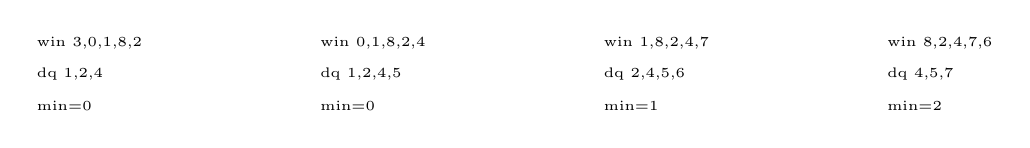
\begin{tikzpicture}[font=\footnotesize]
% F6.3 deque slide on {3,0,1,8,2,4,7,6}, k=5: real index traces.
% dq lists the index stack after each window closes.
\foreach \f/\w/\dq/\mn in {0/{3,0,1,8,2}/{1,2,4}/{0},
  1/{0,1,8,2,4}/{1,2,4,5}/{0},
  2/{1,8,2,4,7}/{2,4,5,6}/{1},
  3/{8,2,4,7,6}/{4,5,7}/{2}}{
  \begin{scope}[xshift=\f*3.6cm]
    \node[font=\tiny,anchor=west] at (0,0) {win \w};
    \node[font=\tiny,anchor=west] at (0,-0.4) {dq \dq};
    \node[font=\tiny,anchor=west] at (0,-0.8) {min=\mn};
  \end{scope}}
\end{tikzpicture}

\caption{The deque's index march on the CSES sample. Notice expired
indices leave through the front while dominated ones leave through the
back --- two retirements, one structure.}
\label{fig:deque}
\end{figure}

\begin{exercise}[medium]\label{exr:dequestack}
Why does the sliding window need a \emph{deque} rather than the
monotonic stack of Section~\ref{sec:monostack}? Which operation does
the window force that the stack never needed?
\end{exercise}


\begin{figure}[htbp]\centering
% fig102-fenwquery.tex -- Figure 5.x: Fenwick prefix(7) reads nodes 7, 6, 4.
% fstyle.tex -- shared TikZ styles for the figures of this book (palette from lifeos.sty).
\tikzset{%
  cell/.style={draw=ink, minimum width=7mm, minimum height=6.5mm, inner sep=0pt, font=\footnotesize, fill=white},
  cellh/.style={cell, fill=accentsoft, draw=accent},
  cella/.style={cell, fill=amberbg, draw=amber},
  cellg/.style={cell, fill=goodbg, draw=good},
  cellx/.style={cell, fill=graybg, draw=slate, text=slate},
  vtx/.style={circle, draw=ink, minimum size=6.5mm, inner sep=0pt, font=\footnotesize, fill=white},
  vtxh/.style={vtx, draw=accent, fill=accentsoft},
  vtxa/.style={vtx, draw=amber, fill=amberbg},
  vtxg/.style={vtx, draw=good, fill=goodbg},
  vtxd/.style={vtx, draw=slate, fill=graybg, text=slate},
  lab/.style={font=\footnotesize, text=slate},
  labA/.style={font=\footnotesize, text=accent},
  labM/.style={font=\footnotesize, text=amber},
  idx/.style={font=\tiny, text=slate},
  arr/.style={-{stealth}, thick, ink},
  arrA/.style={-{stealth}, thick, accent},
  arrM/.style={-{stealth}, thick, amber},
  arrG/.style={-{stealth}, thick, good},
  edge/.style={thick, ink},
  edgeA/.style={thick, accent},
  edgeM/.style={thick, amber},
}%
% \cellrow{prefix}{x0}{y}{style}{v0,v1,...}: a row of cells named prefix0, prefix1, ... (pitch 0.75cm)
\providecommand{\cellrow}[5]{\foreach \v [count=\i from 0] in {#5} {\node[#4] (#1\i) at (#2+\i*0.75,#3) {\v};}}%
% \cellidx{prefix}{n}{start}: index labels under cells prefix0 .. prefix(n-1)
\providecommand{\cellidx}[3]{\foreach \i in {0,...,\numexpr#2-1\relax} {\node[idx, below=0pt of #1\i] {\the\numexpr\i+#3\relax};}}%
% \fitfig{<tikzpicture>}: shrink the picture to \linewidth only when it would overflow.
\ifdefined\fitbox\else\newsavebox{\fitbox}\fi%
\providecommand{\fitfig}[1]{\sbox{\fitbox}{#1}\ifdim\wd\fitbox>\linewidth\resizebox{\linewidth}{!}{\usebox{\fitbox}}\else\usebox{\fitbox}\fi}%

\fitfig{\begin{tikzpicture}[font=\footnotesize, x=1.1cm, y=0.78cm]
\foreach \i/\lb in {1/1,2/2,3/1,4/4,5/1,6/2,7/1,8/8} {
  \pgfmathsetmacro{\lev}{ln(\lb)/ln(2)}
  \pgfmathsetmacro{\lo}{\i-\lb}
  \ifnum\i=7 \def\fillc{amber!25}\def\drc{amber}\else\ifnum\i=6 \def\fillc{amber!25}\def\drc{amber}\else\ifnum\i=4 \def\fillc{amber!25}\def\drc{amber}\else\def\fillc{graybg}\def\drc{slate}\fi\fi\fi
  \draw[draw=\drc, fill=\fillc] (\lo+0.06,\lev+0.1) rectangle (\i-0.06,\lev+0.9);
  \node[font=\scriptsize] at ({(\lo+\i)/2},\lev+0.5) {$t[\i]$};}
\foreach \i in {1,...,8} \node[idx, below] at (\i-0.5,0) {\i};
\node[labM, anchor=west, align=left] at (8.4,2.6) {prefix$(7)$: $i=7$, read $t[7]$, $i\leftarrow 7-1=6$;\\ read $t[6]$, $i\leftarrow6-2=4$; read $t[4]$, $i\leftarrow 0$};
\node[lab, anchor=west, align=left] at (8.4,0.9) {node $i$ covers the last $\mathrm{lowbit}(i)$ cells;\\ strip the lowest set bit each step};
\end{tikzpicture}}

\caption{Fenwick decomposition: prefix($7$) touches nodes $7,6,4$ --- strip the lowbit each step.}
\label{fig:fenwquery}
\end{figure}

\section{Sparse tables: idempotent queries in \texorpdfstring{$O(1)$}{O(1)}}\label{sec:sparse}
\index{sparse table}\index{idempotent}

For a \emph{static} array, a sparse table precomputes the answer on
every interval of length $2^j$: level $j$ holds $n - 2^j + 1$ entries,
each built from two level-$(j{-}1)$ halves, $O(n \log n)$ total. Any
range $[l,r]$ is the union of two overlapping power-of-two pieces
anchored at $l$ and $r$ --- correct precisely when the operation is
\emph{idempotent} ($f(x,x) = x$: $\min$, $\max$, $\gcd$, bitwise
\textsc{and}), because the overlap is then double-counted harmlessly.
A sum double-counts: sparse tables are the wrong tool for range sums.

\begin{lstlisting}[language=C++,caption={\texttt{sparse.h}: $O(n\log n)$
build, $O(1)$ query.},label={lst:sparse}]
\end{lstlisting}
\lstinputlisting{code/sparse.h}

\begin{example}[CSES \emph{Static Range Minimum Queries}]\label{ex:rmq}
Same shape as Chapter~5's sum queries, but minimum: $n,q \le
2\cdot10^5$.
\par\smallskip
\textbf{Strategy.} Prefix tricks fail --- $\min$ has no inverse to
subtract with. But $\min$ \emph{is} idempotent, so two overlapping
precomputed halves cover any range exactly: sparse table.
\par\smallskip
\begin{solution}
\lstinputlisting{code/rmq.cpp}
Real output (CSES sample):
\begin{lstlisting}[numbers=none]
2
1
1
4
\end{lstlisting}
\end{solution}
\end{example}

\begin{example}[CSES \emph{Josephus Problem I}: the queue does the rotating]
\label{ex:joseph}
Children $1..n$ stand in a circle; walking clockwise, every second
remaining child leaves. Print the removal order ($n \le 2\cdot10^5$).
\emph{Input:} \texttt{7}. \emph{Output:} \texttt{2 4 6 1 5 3 7}.
\par\smallskip
\textbf{Strategy.} Simulate the circle directly with the structure built
for it: a \texttt{queue}. Pop the front child; if the step is ``skip'',
push him to the back (he survives this round); if ``eliminate'', print
and drop. Every queue operation is $O(1)$ and each of the $n$ children
is pushed at most $n$ times across the whole run --- amortized linear
work, the theme of this chapter applied to a data structure you already
own. A \texttt{vector} version needs an index walk and wrap-around; the
queue version needs none of it because the circle \emph{is} the
enqueue/dequeue discipline.
\par\smallskip
\begin{solution}
\texttt{code/josephus1.cpp} prints \texttt{2 4 6 1 5 3 7} on the
sample: odd positions leave first in order, then the rotation
re-eliminates among survivors. No arithmetic beyond a toggle flag ---
the amortized cost of ``rotate and inspect'' is the point.
\end{solution}
\end{example}

\begin{figure}[ht]\centering
% fig27-sparse.tex -- Figure 6.4: sparse-table (min) levels over {3,2,4,5,1,1,5,3}; query [1,6] = two level-2 cells.
% fstyle.tex -- shared TikZ styles for the figures of this book (palette from lifeos.sty).
\tikzset{%
  cell/.style={draw=ink, minimum width=7mm, minimum height=6.5mm, inner sep=0pt, font=\footnotesize, fill=white},
  cellh/.style={cell, fill=accentsoft, draw=accent},
  cella/.style={cell, fill=amberbg, draw=amber},
  cellg/.style={cell, fill=goodbg, draw=good},
  cellx/.style={cell, fill=graybg, draw=slate, text=slate},
  vtx/.style={circle, draw=ink, minimum size=6.5mm, inner sep=0pt, font=\footnotesize, fill=white},
  vtxh/.style={vtx, draw=accent, fill=accentsoft},
  vtxa/.style={vtx, draw=amber, fill=amberbg},
  vtxg/.style={vtx, draw=good, fill=goodbg},
  vtxd/.style={vtx, draw=slate, fill=graybg, text=slate},
  lab/.style={font=\footnotesize, text=slate},
  labA/.style={font=\footnotesize, text=accent},
  labM/.style={font=\footnotesize, text=amber},
  idx/.style={font=\tiny, text=slate},
  arr/.style={-{stealth}, thick, ink},
  arrA/.style={-{stealth}, thick, accent},
  arrM/.style={-{stealth}, thick, amber},
  arrG/.style={-{stealth}, thick, good},
  edge/.style={thick, ink},
  edgeA/.style={thick, accent},
  edgeM/.style={thick, amber},
}%
% \cellrow{prefix}{x0}{y}{style}{v0,v1,...}: a row of cells named prefix0, prefix1, ... (pitch 0.75cm)
\providecommand{\cellrow}[5]{\foreach \v [count=\i from 0] in {#5} {\node[#4] (#1\i) at (#2+\i*0.75,#3) {\v};}}%
% \cellidx{prefix}{n}{start}: index labels under cells prefix0 .. prefix(n-1)
\providecommand{\cellidx}[3]{\foreach \i in {0,...,\numexpr#2-1\relax} {\node[idx, below=0pt of #1\i] {\the\numexpr\i+#3\relax};}}%
% \fitfig{<tikzpicture>}: shrink the picture to \linewidth only when it would overflow.
\ifdefined\fitbox\else\newsavebox{\fitbox}\fi%
\providecommand{\fitfig}[1]{\sbox{\fitbox}{#1}\ifdim\wd\fitbox>\linewidth\resizebox{\linewidth}{!}{\usebox{\fitbox}}\else\usebox{\fitbox}\fi}%

\begin{tikzpicture}[font=\footnotesize]
\newcommand{\lev}[3]{% level j, list of values, style
  \foreach \v [count=\i from 0] in {#2}
    \node[#3, minimum width=6.5mm] (s#1-\i) at ({(\i+(2^#1-1)/2)*0.75}, {-#1*0.9}) {\v};
  \node[lab, anchor=east] at (-0.5,{-#1*0.9}) {$j{=}#1$};}
\lev{0}{3,2,4,5,1,1,5,3}{cell}
\lev{1}{2,2,4,1,1,1,3}{cellx}
\lev{2}{2,1,1,1,1}{cellx}
\lev{3}{1}{cellx}
\foreach \i in {1,...,6} \draw[amber, very thick] (s0-\i.south west) rectangle (s0-\i.north east);
\foreach \i in {1,3} \draw[amber, very thick, fill=amberbg] (s2-\i.south west) rectangle (s2-\i.north east);
\node at (s2-1) {1}; \node at (s2-3) {1};
\node[labM, align=left, anchor=west] at (7.0,-1.8) {query $\min a[1..6]$: length 6,\\ $j=2$, read two cells\\ $\min(\text{level}_2[1],\text{level}_2[3])=1$};
\end{tikzpicture}

\caption{Sparse-table levels over $\{3,2,4,5,1,1,5,3\}$. Notice level
$j$'s $i$-th cell already contains the answer for the whole
$2^j$-block starting at $i$ --- a query is two reads, never more.}
\label{fig:sparse}
\end{figure}

\begin{exercise}[medium]\label{exr:idem}
Which of $\{\min, \max, \gcd, \mathrm{sum}, \mathrm{xor},
\mathrm{lcm}\}$ are idempotent --- i.e., safe for the sparse table's
two-piece query? For each unsafe one, name the query where overlap
double-counts.
\end{exercise}

\section{Square roots: the good-enough structure}\label{sec:sqrt}
\index{square-root decomposition}

When the array \emph{does} change, split it into $B \approx \sqrt n$
blocks with a stored sum per block. A range sum reads whole blocks in
$O(1)$ each and scans at most two partial fringes: $O(\sqrt n)$ per
query, $O(1)$ per point update. That is worse than a segment tree's
$O(\log n)$ --- and often the right trade anyway: the code is a page
of loops with no recursion, no trees, and no subtle bugs at 2\,a.m.

\begin{lstlisting}[language=C++,caption={\texttt{sqrtdec.h}: block sums
plus point updates.},label={lst:sqrtdec}]
\end{lstlisting}
\lstinputlisting{code/sqrtdec.h}

\begin{lstlisting}[numbers=none,caption={\texttt{sqrt\_sum.cpp} real
output.},label={lst:sqrtout}]
sum[2..6] = 21
after set(4,0): sum[2..6] = 16
sum[0..9] = 34
\end{lstlisting}

\begin{figure}[ht]\centering
\begin{tikzpicture}[font=\footnotesize,x=0.5cm]
% F6.5 sqrt buckets: [3,1,4|1,5,9|2,6,5|3] sums 8/15/13/3.
\foreach \i/\v in {0/3,1/1,2/4,3/1,4/5,5/9,6/2,7/6,8/5,9/3}
  \node[draw=slate,minimum width=0.42cm,minimum height=0.4cm,font=\tiny]
    at (\i*0.48,0) {\v};
\foreach \b/\s in {0/8,1/15,2/13,3/3}
  \node[draw=accent,fill=accentsoft,font=\tiny] at (\b*1.44+0.55,0.75) {\s};
\draw[decorate,decoration={brace,raise=2pt}] (0,0.95) -- (1.44,0.95);
\draw[decorate,decoration={brace,raise=2pt}] (1.5,0.95) -- (2.94,0.95);
\draw[decorate,decoration={brace,raise=2pt}] (3.0,0.95) -- (4.4,0.95);
\node[font=\tiny] at (2.4,-0.7) {fringe cells scanned; whole blocks
summed in one read};
\end{tikzpicture}

\caption{Block sums over 3-blocks. Notice a query touches at most two
scanned fringes; everything in between is one table read per block.}
\label{fig:sqrt}
\end{figure}

\section{Chapter summary}
\begin{table}[ht]\centering
{\small
\begin{tabularx}{\linewidth}{@{}lYYY@{}}
\toprule
\tablehead\thead{Structure} & \thead{Answers} & \thead{Cost} & \thead{Needs}\\
\midrule
monotonic stack & nearest smaller/greater & $O(n)$ total & one pass\\
monotonic deque & sliding-window min/max & $O(n)$ & window slides\\
sparse table & static range min/max/gcd & $O(1)$ query & idempotent op\\
sqrt blocks & range sum + updates & $O(\sqrt n)$ & simplicity\\
\bottomrule
\end{tabularx}}
\caption{All four are the same accounting: charge the element, not the
call --- and read the operation's algebra before choosing.}
\label{tab:amort}
\end{table}

\section{Common mistakes}
\index{common mistakes}
\begin{itemize}
\item \textbf{Sparse table on a non-idempotent op.} Two overlapping
pieces are only safe when $f(x,x)=x$; a sparse table for range sum
double-counts the overlap and silently returns wrong answers.
\item \textbf{Forgetting the expiry check.} The deque's front must be
evicted when it leaves the window --- separate from the domination
pop; skipping it returns the minimum of a window that no longer
exists.
\item \textbf{Counting pops per call.} Amortised bounds are proven on
the \emph{sequence}, not the operation: ``one push can pop $k$'' is
fine because each index is popped at most once ever.
\item \textbf{Strictness flips.} $\ge$ vs $>$ in the pop condition
decides whether equal values count as ``smaller-or-equal neighbours'';
pick per the statement and test on duplicates.
\item \textbf{Block-size blind spots.} The fringe scan is $O(B)$ ---
queries shorter than $B$ inside one block must take the scalar path
(handled by the $bl = br$ branch); skipping it sums whole blocks for a
two-cell query.
\end{itemize}

\section{Additional exercises}
\begin{exercise}[easy]
CSES \emph{Towers} --- longest non-increasing run per cube
(\texttt{upper\_bound} or monotonic multiset).
\end{exercise}

\begin{exercise}[easy]
USACO-S \emph{Convention II} --- sorted queue mechanics.
\end{exercise}
\begin{exercise}[easy]
LC \emph{IPO} --- two heaps as amortised selection.
\end{exercise}
\begin{exercise}[medium]
CSES \emph{Traffic Lights} --- ordered set of segments.
\end{exercise}
\begin{exercise}[medium]
CSES \emph{Josephus Problem II} --- order-statistics elimination.
\end{exercise}
\begin{exercise}[medium]
USACO-S \emph{Milk Measurement} --- ordered leaderboard updates.
\end{exercise}
\begin{exercise}[medium]
CF \emph{William and Robot} --- greedy selection structure.
\end{exercise}
\begin{exercise}[easy] CSES \emph{Playlist} --- the sliding window with a set membership test. \end{exercise}
\begin{exercise}[easy] CSES \emph{Range Xor Queries} --- xor prefix; why does the same trick work? \end{exercise}
\begin{exercise}[medium] Derive the amortized bound for a queue built from two stacks: assign each element a potential. \end{exercise}
\begin{exercise}[medium] Implement sliding-window minimum with a plain array + head index (no \texttt{deque}); verify against the deque version. \end{exercise}
\begin{exercise}[hard]
CSES \emph{Stick Division} --- heap-of-two-smallest merges (Huffman).
\end{exercise}
\begin{exercise}[hard]
USACO-S \emph{Deforestation} --- range constraints + structure choice.
\end{exercise}
\begin{exercise}[hard]
USACO-G \emph{Job Completion} --- multi-structure scheduling.
\end{exercise}

\chapternotes
The amortised-accounting framing follows Sannemo's structures
sections~\cite{sannemo2025} and Laaksonen's data-structures
chapter~\cite{laaksonen2024}; the USACO Guide's Silver/Gold modules
carry the monotonic-stack and deque drills~\cite{usacoguide}, and
cp-algorithms documents the sparse table's idempotency
requirement~\cite{cpalgorithms}. Halim~\cite{halimcp4} covers the
same set with contest IDs; the archive problems are official
CSES/USACO tasks~\cite{cses}.
\begin{exercise}[hard] USACO-G \emph{Haybale Feast} --- monotonic deque with a sum constraint. \end{exercise}

\section*{Further reading}
\begin{itemize}
\item cp-algorithms, ``Sparse table'' (intermediate) ---
the static RMQ structure of \S\ref{sec:sparse} with disjoint-range
queries beyond min. \newline\url{https://cp-algorithms.com/data_structures/sparse-table.html}
\item cp-algorithms, ``Modifying stack/queue for minimum queries''
(intermediate). (article: ``Minimum stack / minimum queue)
--- the monotonic queue of \S\ref{sec:monodeque} derived twice over
(stack-pair and deque). \newline\url{https://cp-algorithms.com/}
\item Laaksonen, \emph{Competitive Programmer's Handbook}, ch.~8
``Amortized analysis'' (beginner).
--- the accounting argument behind \S\ref{sec:amort}. \newline\url{https://cses.fi/book/book.pdf}
\item CSES 1645 \emph{Nearest Smaller Values} (practice) --- \ref{ex:nsv} verbatim;
the canonical monotonic-stack submission. \newline\url{https://cses.fi/problemset/task/1645}
\item CSES 1647 \emph{Static Range Minimum Queries} (practice) --- where the sparse table
of \ref{ex:rmq} earns its keep. \newline\url{https://cses.fi/problemset/task/1647}
\item Wikipedia, ``Amortized analysis'' (reference) --- aggregate /
accounting / potential methods; the book uses the aggregate version. \newline\url{https://en.wikipedia.org/wiki/Amortized_analysis}\end{itemize}

\begin{rulebox}[Watch instead]
\smallskip\noindent\textbf{Best first.}
``Monotonic Stack Data Structure Explained'' --- AlgoMonster, 6 min ---
\url{https://youtu.be/Dq_ObZwTY_Q}. The
pop-while-monotone loop of \S\ref{sec:monostack} on next-greater-element;
pseudocode-style, no language dependency.
\smallskip\noindent
``Sparse Table | Range Minimum Query in O(1)'' --- Kartik Arora,
17 min --- \url{https://youtu.be/iaRvydtqLV4}. Builds
exactly the $k$-level table of \S\ref{sec:sparse} then answers
$[\ell,r]$ via the two overlapping power-of-2 blocks; uses
$\lfloor\log_2(r-\ell+1)\rfloor$ like the book. Access date 2026-10-10.
\end{rulebox}

\chapter{Graphs: traversal and order}\label{ch:graphs}
\index{graph traversal}\index{DFS}\index{BFS}\index{topological sort}

Every graph problem in this book reduces to one question first: what
order do I visit the vertices? Depth-first search dives until stuck
and unrolls the answer on the way back; breadth-first search expands
in layers and thereby measures unweighted distance for free. Built on
them: flood fill for grids, two-colouring for bipartite checks,
Kahn's algorithm for ordering a DAG, and the tail-plus-cycle anatomy
of functional graphs. After this chapter you will choose the
traversal that makes the needed invariant fall out, write the
adjacency-list idiom without thinking, and reconstruct answers ---
paths, components, orders --- from the arrays the search leaves
behind.

\section{Vocabulary}\label{sec:vocab}\index{graph!vocabulary}
A graph $G = (V,E)$ is vertices plus edges: undirected pairs
$\{u,v\}$, or directed arcs $(u,v)$, possibly weighted. Degree counts
incident edges. A \emph{path} revisits nothing; a \emph{cycle}
returns; connected pieces are \emph{components}. Directed graphs get
their own adjectives: a DAG is acyclic; functional graphs have
out-degree exactly 1.

\section{Representations: adjacency lists only}\label{sec:repr}
\index{adjacency list}
The contest representation is \texttt{vector<vector<int>> g(n+1)}:
memory $O(V{+}E)$, iteration $O(\deg v)$. Adjacency \emph{matrices}
cost $O(V^2)$ and are only for dense tiny graphs. Three traps:
self-loops and multi-edges are legal input (your code must not assume
otherwise); CSES vertices are 1-indexed (size the array $n{+}1$); and
undirected edges are added \emph{both} ways.
\begin{figure}[ht]\centering
% fig29-adjlist.tex -- Figure 7.1: the same triangle as a drawing and as adjacency lists.
% fstyle.tex -- shared TikZ styles for the figures of this book (palette from lifeos.sty).
\tikzset{%
  cell/.style={draw=ink, minimum width=7mm, minimum height=6.5mm, inner sep=0pt, font=\footnotesize, fill=white},
  cellh/.style={cell, fill=accentsoft, draw=accent},
  cella/.style={cell, fill=amberbg, draw=amber},
  cellg/.style={cell, fill=goodbg, draw=good},
  cellx/.style={cell, fill=graybg, draw=slate, text=slate},
  vtx/.style={circle, draw=ink, minimum size=6.5mm, inner sep=0pt, font=\footnotesize, fill=white},
  vtxh/.style={vtx, draw=accent, fill=accentsoft},
  vtxa/.style={vtx, draw=amber, fill=amberbg},
  vtxg/.style={vtx, draw=good, fill=goodbg},
  vtxd/.style={vtx, draw=slate, fill=graybg, text=slate},
  lab/.style={font=\footnotesize, text=slate},
  labA/.style={font=\footnotesize, text=accent},
  labM/.style={font=\footnotesize, text=amber},
  idx/.style={font=\tiny, text=slate},
  arr/.style={-{stealth}, thick, ink},
  arrA/.style={-{stealth}, thick, accent},
  arrM/.style={-{stealth}, thick, amber},
  arrG/.style={-{stealth}, thick, good},
  edge/.style={thick, ink},
  edgeA/.style={thick, accent},
  edgeM/.style={thick, amber},
}%
% \cellrow{prefix}{x0}{y}{style}{v0,v1,...}: a row of cells named prefix0, prefix1, ... (pitch 0.75cm)
\providecommand{\cellrow}[5]{\foreach \v [count=\i from 0] in {#5} {\node[#4] (#1\i) at (#2+\i*0.75,#3) {\v};}}%
% \cellidx{prefix}{n}{start}: index labels under cells prefix0 .. prefix(n-1)
\providecommand{\cellidx}[3]{\foreach \i in {0,...,\numexpr#2-1\relax} {\node[idx, below=0pt of #1\i] {\the\numexpr\i+#3\relax};}}%
% \fitfig{<tikzpicture>}: shrink the picture to \linewidth only when it would overflow.
\ifdefined\fitbox\else\newsavebox{\fitbox}\fi%
\providecommand{\fitfig}[1]{\sbox{\fitbox}{#1}\ifdim\wd\fitbox>\linewidth\resizebox{\linewidth}{!}{\usebox{\fitbox}}\else\usebox{\fitbox}\fi}%

\begin{tikzpicture}[font=\footnotesize]
\node[vtx] (v1) at (0,1.5) {1}; \node[vtx] (v2) at (1.8,1.5) {2}; \node[vtx] (v3) at (0.9,0) {3};
\draw[edge] (v1)--(v2) (v2)--(v3) (v1)--(v3);
\node[lab] at (0.9,-0.9) {triangle: 3 edges};
\node[lab, anchor=east] at (4.6,1.5) {};
\foreach \n/\l [count=\k from 0] in {1/{2,3},2/{1,3},3/{1,2}} {
  \node[cellh, minimum width=6mm] (h\n) at (5.4,1.5-\k*0.85) {\n};
  \node[lab, left=1pt of h\n] {};
  \foreach \t [count=\j from 1] in \l
    \node[cell, minimum width=6mm] (e\n\j) at (5.4+\j*1.0,1.5-\k*0.85) {\t};
  \draw[arr] (h\n) -- (e\n1); \draw[arr] (e\n1) -- (e\n2);
}
\node[lab] at (6.5,-1.0) {adjacency lists: each edge stored twice};
\end{tikzpicture}

\caption{The same triangle two ways. Notice the lists store each edge
twice --- that's the price of $O(\deg v)$ iteration.}
\label{fig:adjlist}
\end{figure}

\section{Depth-first search}\label{sec:dfs}
DFS recurses into the first unseen neighbour; the visited set makes
each vertex processed once, so a full pass is $O(V{+}E)$. Free
applications: component counting (one outer call per component),
reachability, cycle detection by back-edge, and --- on grids ---
flood fill.
\begin{lstlisting}[language=C++,caption={\texttt{dfs.h}: the five-line
idiom.},label={lst:dfs}]
\end{lstlisting}
\lstinputlisting{code/dfs.h}
\begin{figure}[ht]\centering
% fig30-dfsstack.tex -- Figure 7.2: DFS recursion stack on the path A - B - D.
% fstyle.tex -- shared TikZ styles for the figures of this book (palette from lifeos.sty).
\tikzset{%
  cell/.style={draw=ink, minimum width=7mm, minimum height=6.5mm, inner sep=0pt, font=\footnotesize, fill=white},
  cellh/.style={cell, fill=accentsoft, draw=accent},
  cella/.style={cell, fill=amberbg, draw=amber},
  cellg/.style={cell, fill=goodbg, draw=good},
  cellx/.style={cell, fill=graybg, draw=slate, text=slate},
  vtx/.style={circle, draw=ink, minimum size=6.5mm, inner sep=0pt, font=\footnotesize, fill=white},
  vtxh/.style={vtx, draw=accent, fill=accentsoft},
  vtxa/.style={vtx, draw=amber, fill=amberbg},
  vtxg/.style={vtx, draw=good, fill=goodbg},
  vtxd/.style={vtx, draw=slate, fill=graybg, text=slate},
  lab/.style={font=\footnotesize, text=slate},
  labA/.style={font=\footnotesize, text=accent},
  labM/.style={font=\footnotesize, text=amber},
  idx/.style={font=\tiny, text=slate},
  arr/.style={-{stealth}, thick, ink},
  arrA/.style={-{stealth}, thick, accent},
  arrM/.style={-{stealth}, thick, amber},
  arrG/.style={-{stealth}, thick, good},
  edge/.style={thick, ink},
  edgeA/.style={thick, accent},
  edgeM/.style={thick, amber},
}%
% \cellrow{prefix}{x0}{y}{style}{v0,v1,...}: a row of cells named prefix0, prefix1, ... (pitch 0.75cm)
\providecommand{\cellrow}[5]{\foreach \v [count=\i from 0] in {#5} {\node[#4] (#1\i) at (#2+\i*0.75,#3) {\v};}}%
% \cellidx{prefix}{n}{start}: index labels under cells prefix0 .. prefix(n-1)
\providecommand{\cellidx}[3]{\foreach \i in {0,...,\numexpr#2-1\relax} {\node[idx, below=0pt of #1\i] {\the\numexpr\i+#3\relax};}}%
% \fitfig{<tikzpicture>}: shrink the picture to \linewidth only when it would overflow.
\ifdefined\fitbox\else\newsavebox{\fitbox}\fi%
\providecommand{\fitfig}[1]{\sbox{\fitbox}{#1}\ifdim\wd\fitbox>\linewidth\resizebox{\linewidth}{!}{\usebox{\fitbox}}\else\usebox{\fitbox}\fi}%

\begin{tikzpicture}[font=\footnotesize]
% frame: x, number of stack entries, current vertex (A/B/D), caption
\newcommand{\fr}[4]{%
  \node[\ifnum#2>0 vtxh\else vtx\fi] (A#4) at (#1,2.4) {A};
  \node[\ifnum#2>1 vtxh\else vtx\fi] (B#4) at (#1+0.9,2.4) {B};
  \node[\ifnum#2>2 vtxh\else vtx\fi] (D#4) at (#1+1.8,2.4) {D};
  \draw[edge] (A#4)--(B#4)--(D#4);
  \foreach \l [count=\k from 0] in {A,B,D} {%
    \ifnum\k<#2 \node[cellh, minimum width=9mm] at (#1+0.9,0.4+\k*0.7) {\l};\fi}
  \draw[slate] (#1+0.35,0) -- (#1+0.35,2.0) -- ++(0,0) (#1+1.45,0) -- (#1+1.45,2.0) (#1+0.35,0) -- (#1+1.45,0);
  \node[lab, align=center, text width=2.6cm] at (#1+0.9,-0.65) {#3};}
\fr{0}{1}{call A: depth 1}{1}
\fr{3.6}{2}{call B: depth 2}{2}
\fr{7.2}{3}{call D: depth 3}{3}
\fr{10.8}{2}{D returns: pop}{4}
\end{tikzpicture}

\caption{The recursion stack growing and unwinding. Notice vertices
\emph{stay} on the stack while their subtree is explored --- that
resident set is what makes back-edge detection work.}
\label{fig:dfsstack}
\end{figure}

\section{Breadth-first search}\label{sec:bfs}
BFS dequeues in arrival order, so vertices surface in nondecreasing
distance: \texttt{dist[]} is the true unweighted shortest path, and
\texttt{parent[]} reconstructs it backwards.
\begin{lstlisting}[language=C++,caption={\texttt{bfs.h}: dist +
parent, the reconstruction pair.},label={lst:bfs}]
\end{lstlisting}
\lstinputlisting{code/bfs.h}
\begin{figure}[ht]\centering
\begin{tikzpicture}[font=\footnotesize]
% F7.3 BFS waves: 4 frames, vertices lit when dequeued.
\begin{scope}
  \node[circle,draw=slate,fill=accentsoft,font=\tiny] at (1.1,1.0) {s};
  \node[circle,draw=slate,font=\tiny] at (0.4,0.2) {};
  \node[circle,draw=slate,font=\tiny] at (1.1,0.2) {};
  \node[circle,draw=slate,font=\tiny] at (1.8,0.2) {};
  \node[font=\tiny] at (1.1,-0.5) {wave 0: \{s\}};
\end{scope}
\begin{scope}[xshift=3.2cm]
  \node[circle,draw=slate,fill=graybg,font=\tiny] at (1.1,1.0) {s};
  \node[circle,draw=slate,fill=accentsoft,font=\tiny] at (0.4,0.2) {};
  \node[circle,draw=slate,fill=accentsoft,font=\tiny] at (1.1,0.2) {};
  \node[circle,draw=slate,fill=accentsoft,font=\tiny] at (1.8,0.2) {};
  \node[font=\tiny] at (1.1,-0.5) {wave 1};
\end{scope}
\begin{scope}[xshift=6.4cm]
  \node[circle,draw=slate,fill=graybg,font=\tiny] at (1.1,1.0) {s};
  \node[circle,draw=slate,fill=graybg,font=\tiny] at (0.4,0.2) {};
  \node[circle,draw=slate,fill=graybg,font=\tiny] at (1.1,0.2) {};
  \node[circle,draw=slate,fill=accentsoft,font=\tiny] at (1.8,0.2) {};
  \node[circle,draw=slate,fill=accentsoft,font=\tiny] at (2.6,0.2) {};
  \node[font=\tiny] at (1.5,-0.5) {wave 2};
\end{scope}
\begin{scope}[xshift=10.2cm]
  \node[circle,draw=slate,fill=graybg,font=\tiny] at (1.1,1.0) {s};
  \node[circle,draw=slate,fill=graybg,font=\tiny] at (0.4,0.2) {};
  \node[circle,draw=slate,fill=graybg,font=\tiny] at (1.1,0.2) {};
  \node[circle,draw=slate,fill=graybg,font=\tiny] at (1.8,0.2) {};
  \node[circle,draw=slate,fill=graybg,font=\tiny] at (2.6,0.2) {};
  \node[font=\tiny] at (1.5,-0.5) {wave 3: done};
\end{scope}
\end{tikzpicture}

\caption{BFS as expanding waves. Notice every vertex in wave $k$ is
exactly distance $k$ --- the queue order \emph{is} the distance
order.}
\label{fig:bfslayers}
\end{figure}
\begin{example}[CSES \emph{Labyrinth}]\label{ex:labyrinth}
Shortest path through a grid with walls; output the path itself.
\par\smallskip
\textbf{Strategy.} ``Shortest'' and ``unweighted'' together name BFS.
The path is recovered by walking \texttt{parent} from the goal ---
search forward, reconstruct backward.
\par\smallskip
\begin{solution}
\lstinputlisting{code/labyrinth.cpp}
Real output (CSES sample):
\begin{lstlisting}[numbers=none]
YES
9
LDDRRRRRU
\end{lstlisting}
\end{solution}
\end{example}

\section{Flood fill}\label{sec:flood}\index{flood fill}
A grid is an implicit graph: cells are vertices, the four directions
are edges. Flood fill counts components --- and uses an
\emph{explicit} stack, because a 1000$\times$1000 room is a million
frames deep.
\begin{lstlisting}[language=C++,caption={\texttt{floodfill.h}:
iterative, 4-direction, marks by rewriting the grid.},label={lst:flood}]
\end{lstlisting}
\lstinputlisting{code/floodfill.h}
\begin{example}[CSES \emph{Counting Rooms}]\label{ex:rooms}
Count floor-connected regions.
\par\smallskip
\textbf{Strategy.} Every unvisited floor cell starts a new room; fill
it completely before moving on. Component counting is the outer loop
--- the fill is just DFS wearing grid clothes.
\par\smallskip
\begin{solution}
\lstinputlisting{code/counting_rooms.cpp}
Real output (CSES sample):
\begin{lstlisting}[numbers=none]
3
\end{lstlisting}
\end{solution}
\end{example}
\begin{figure}[ht]\centering
% fig32-gridgraph.tex -- Figure 7.4: a grid cell as a vertex with four computed neighbours.
% fstyle.tex -- shared TikZ styles for the figures of this book (palette from lifeos.sty).
\tikzset{%
  cell/.style={draw=ink, minimum width=7mm, minimum height=6.5mm, inner sep=0pt, font=\footnotesize, fill=white},
  cellh/.style={cell, fill=accentsoft, draw=accent},
  cella/.style={cell, fill=amberbg, draw=amber},
  cellg/.style={cell, fill=goodbg, draw=good},
  cellx/.style={cell, fill=graybg, draw=slate, text=slate},
  vtx/.style={circle, draw=ink, minimum size=6.5mm, inner sep=0pt, font=\footnotesize, fill=white},
  vtxh/.style={vtx, draw=accent, fill=accentsoft},
  vtxa/.style={vtx, draw=amber, fill=amberbg},
  vtxg/.style={vtx, draw=good, fill=goodbg},
  vtxd/.style={vtx, draw=slate, fill=graybg, text=slate},
  lab/.style={font=\footnotesize, text=slate},
  labA/.style={font=\footnotesize, text=accent},
  labM/.style={font=\footnotesize, text=amber},
  idx/.style={font=\tiny, text=slate},
  arr/.style={-{stealth}, thick, ink},
  arrA/.style={-{stealth}, thick, accent},
  arrM/.style={-{stealth}, thick, amber},
  arrG/.style={-{stealth}, thick, good},
  edge/.style={thick, ink},
  edgeA/.style={thick, accent},
  edgeM/.style={thick, amber},
}%
% \cellrow{prefix}{x0}{y}{style}{v0,v1,...}: a row of cells named prefix0, prefix1, ... (pitch 0.75cm)
\providecommand{\cellrow}[5]{\foreach \v [count=\i from 0] in {#5} {\node[#4] (#1\i) at (#2+\i*0.75,#3) {\v};}}%
% \cellidx{prefix}{n}{start}: index labels under cells prefix0 .. prefix(n-1)
\providecommand{\cellidx}[3]{\foreach \i in {0,...,\numexpr#2-1\relax} {\node[idx, below=0pt of #1\i] {\the\numexpr\i+#3\relax};}}%
% \fitfig{<tikzpicture>}: shrink the picture to \linewidth only when it would overflow.
\ifdefined\fitbox\else\newsavebox{\fitbox}\fi%
\providecommand{\fitfig}[1]{\sbox{\fitbox}{#1}\ifdim\wd\fitbox>\linewidth\resizebox{\linewidth}{!}{\usebox{\fitbox}}\else\usebox{\fitbox}\fi}%

\begin{tikzpicture}[font=\footnotesize, x=1.15cm, y=0.85cm]
\foreach \x in {0,...,4} \foreach \y in {0,...,3} \draw[slate!60, fill=white] (\x,\y) rectangle +(1,1);
\fill[amber!25] (1,1) rectangle +(1,1);
\foreach \x/\y in {1/2,1/0,0/1,2/1} \fill[accentsoft] (\x,\y) rectangle +(1,1);
\foreach \x in {0,...,4} \foreach \y in {0,...,3} \draw[slate!60] (\x,\y) rectangle +(1,1);
\node[font=\scriptsize] at (1.5,1.5) {$(r,c)$};
\node[font=\scriptsize] at (1.5,2.5) {$(r{-}1,c)$}; \node[font=\scriptsize] at (1.5,0.5) {$(r{+}1,c)$};
\node[font=\scriptsize] at (0.5,1.5) {$(r,c{-}1)$}; \node[font=\scriptsize] at (2.5,1.5) {$(r,c{+}1)$};
\node[lab, align=left, anchor=west] at (5.6,2.5) {one floor cell $=$ one vertex};
\node[lab, align=left, anchor=west] at (5.6,1.5) {4 neighbours by the direction\\ arrays \texttt{dr}, \texttt{dc}};
\node[lab, align=left, anchor=west] at (5.6,0.5) {no graph is stored:\\ neighbours are computed};
\end{tikzpicture}

\caption{One cell, four edges. Notice there is no graph object ---
the neighbours are computed, never stored.}
\label{fig:gridgraph}
\end{figure}

\section{Bipartite checks}\label{sec:bip}\index{bipartite}
Colour as you traverse: every neighbour gets the opposite colour, and
the first conflict certifies an odd cycle. If a pass completes, the
colouring itself is the proof.
\begin{example}[CSES \emph{Building Teams}]\label{ex:teams}
Split pupils so friends land on different teams.
\par\smallskip
\textbf{Strategy.} ``Two groups, no inside edges'' is bipartiteness
rephrased; BFS two-colouring either emits the split or meets its own
edge and prints IMPOSSIBLE.
\par\smallskip
\begin{solution}
\lstinputlisting{code/building_teams.cpp}
Real output (CSES sample):
\begin{lstlisting}[numbers=none]
1 2 2 1 2
\end{lstlisting}
\end{solution}
\end{example}

\section{Directed order: Kahn and the DAG}\label{sec:topo}\index{Kahn's algorithm}\index{topological order}
A DAG admits an order where every edge points forward. Kahn's
algorithm: emit in-degree-0 vertices, decrement their out-neighbours,
repeat. If the queue empties with vertices left, they are exactly the
cycle-entangled ones --- the algorithm detects cycles for free.
\begin{lstlisting}[language=C++,caption={\texttt{toposort.h}: Kahn;
short order $=$ cycle.},label={lst:kahn}]
\end{lstlisting}
\lstinputlisting{code/toposort.h}
\begin{example}[CSES \emph{Course Schedule}]\label{ex:course}
Order $n$ courses satisfying prerequisites.
\par\smallskip
\textbf{Strategy.} Prerequisite edges are a DAG exactly when the task
is possible; Kahn emits the order or exposes the cycle.
\par\smallskip
\begin{solution}
\lstinputlisting{code/course_schedule.cpp}
Real output (CSES sample, one valid order):
\begin{lstlisting}[numbers=none]
3 4 1 5 2
\end{lstlisting}
\end{solution}
\end{example}
\begin{figure}[ht]\centering
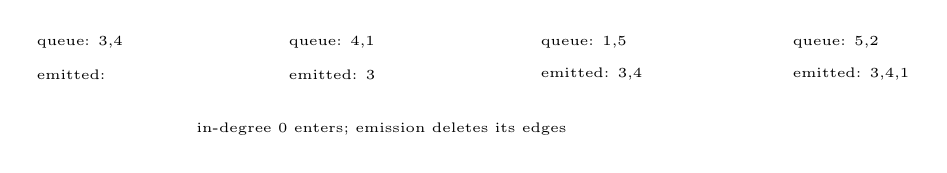
\begin{tikzpicture}[font=\footnotesize]
\foreach \i/\q/\e in {0/{3,4}/{ },1/{4,1}/{3},2/{1,5}/{3,4},3/{5,2}/{3,4,1}}{
  \begin{scope}[xshift=\i*3.2cm]
    \node[font=\tiny,anchor=west] at (0,0.6) {queue: \q};
    \node[font=\tiny,anchor=west] at (0,0.2) {emitted: \e};
  \end{scope}}
\node[font=\tiny] at (4.5,-0.5) {in-degree 0 enters; emission deletes its edges};
\end{tikzpicture}

\caption{Kahn's queue evolution. Notice the emitted sequence is a
\emph{proof}: at print time each vertex's remaining in-degree is 0.}
\label{fig:kahn}
\end{figure}

\section{Functional graphs: tail plus cycle}\label{sec:func}\index{functional graph}
Out-degree 1 means every walk is a tail into a cycle --- the $\rho$
shape of Figure~\ref{fig:rho}. Walks are deterministic, so answers
decompose: distance-to-cycle, then cycle length.
\begin{example}[CSES \emph{Planets Cycles}]\label{ex:planets}
Teleportations until a planet is revisited, per start.
\par\smallskip
\textbf{Strategy.} From any start the trajectory is tail + cycle: the
answer is tail-length + cycle-length. One pass per start, marking as
we go, gives each vertex's answer in $O(n)$ total.
\par\smallskip
\begin{solution}
\lstinputlisting{code/planets_cycles.cpp}
Real output (CSES sample $t=\{2,4,3,1,4\}$):
\begin{lstlisting}[numbers=none]
3 3 1 3 4
\end{lstlisting}
\end{solution}
\end{example}
\begin{figure}[ht]\centering
\begin{tikzpicture}[font=\footnotesize]
\node[circle,draw=slate,font=\tiny] (a) at (0,0) {5};
\node[circle,draw=slate,font=\tiny] (b) at (0.9,0) {4};
\node[circle,draw=slate,fill=accentsoft,font=\tiny] (c) at (1.8,0) {1};
\node[circle,draw=slate,fill=accentsoft,font=\tiny] (d) at (2.7,0.7) {2};
\node[circle,draw=slate,fill=accentsoft,font=\tiny] (e) at (2.7,-0.7) {3};
\draw[-{stealth},slate] (a)--(b) (b)--(c) (c)--(d) (d)--(e) (e)--(c);
\node[font=\tiny] at (0.9,-0.35) {tail};
\node[font=\tiny] at (2.7,1.2) {cycle};
\node[font=\tiny] at (1.4,-1.4) {the $\rho$ shape: every functional
graph is tails feeding cycles};
\end{tikzpicture}

\caption{The $\rho$ anatomy. Notice the tail can be empty --- pure
cycles and self-loops are the same shape with zero stem.}
\label{fig:rho}
\end{figure}

\begin{exercise}[easy]\label{exr:edgecase}
The input may contain a self-loop $(v,v)$ and the parallel edge
$(u,v),(u,v)$. What does each do to your degree counts, BFS layering,
and Kahn's in-degree array?
\end{exercise}
\begin{exercise}[medium]\label{exr:bfsdfs}
On a path graph $1{-}2{-}\cdots{-}n$, state the visit orders of DFS
and BFS from vertex 1. Where do they differ first on a 4-cycle?
\end{exercise}
\begin{exercise}[medium]\label{exr:kahnstop}
Kahn stops early exactly when the leftover subgraph has a directed
cycle. Why can a nonempty acyclic leftover never happen?
\end{exercise}
\begin{exercise}[medium]\label{exr:funcentry}
In a functional graph, show that following successors from any vertex
eventually repeats --- and that the first repeated vertex is always
on the cycle, never mid-tail.
\end{exercise}

\section{Chapter summary}
\begin{table}[ht]\centering
{\small
\begin{tabularx}{\linewidth}{@{}lYYY@{}}
\toprule
\tablehead\thead{Need} & \thead{Tool} & \thead{Cost} & \thead{Leaves behind}\\
\midrule
reach a vertex & DFS & $O(V{+}E)$ & components, order\\
shortest unweighted path & BFS & $O(V{+}E)$ & dist, parent\\
count grid regions & flood fill & $O(nm)$ & painted cells\\
two groups / odd cycle & 2-colour BFS & $O(V{+}E)$ & team array\\
order a DAG & Kahn & $O(V{+}E)$ & topo order or cycle\\
successor structure & walk + stamp & $O(n)$ & tail/cycle split\\
\bottomrule
\end{tabularx}}
\caption{Pick by the invariant you need: layers mean distance, the
stack means depth, the queue's leftovers mean cycles.}
\label{tab:traverse}
\end{table}

\section{Common mistakes}
\index{common mistakes}
\begin{itemize}
\item \textbf{Recursive flood fill on big grids.} $10^6$ cells is a
million-deep call stack --- iterative or explicit-stack only.
\item \textbf{BFS on weighted edges.} Layers are edge \emph{counts};
weights need Dijkstra (Ch~11), and BFS's first visit is no longer
shortest.
\item \textbf{Marking on enqueue vs dequeue.} Mark \texttt{seen} when
\emph{enqueuing}; marking on dequeue lets the same vertex enter the
queue many times --- still correct but quadratic on dense graphs.
\item \textbf{1-indexed off-by-one.} CSES vertices are $1..n$; an
$n$-sized vector drops vertex $n$ silently.
\item \textbf{Forgetting the second direction.} Undirected edges need
two adjacency entries; a one-way insert makes the graph half-directed
and every later claim quietly wrong.
\end{itemize}

\section{Additional exercises}
\begin{exercise}[easy] CSES \emph{Building Roads} --- components + links. \end{exercise}
\begin{exercise}[easy] CSES \emph{Message Route} --- BFS reconstruction. \end{exercise}
\begin{exercise}[easy] USACO-S \emph{Closing the Farm} --- component queries. \end{exercise}
\begin{exercise}[easy] USACO-B \emph{Family Tree} --- ancestor DFS. \end{exercise}
\begin{exercise}[medium] CSES \emph{Round Trip} --- undirected cycle extraction. \end{exercise}
\begin{exercise}[medium] CSES \emph{Game Routes} --- DP on topological order. \end{exercise}
\begin{exercise}[medium] USACO-S \emph{Icy Perimeter} --- flood-fill perimeter. \end{exercise}
\begin{exercise}[medium] USACO-S \emph{Build Gates} --- scaled-cell fill. \end{exercise}
\begin{exercise}[medium] USACO-S \emph{Mooyo Mooyo} --- gravity + fill. \end{exercise}
\begin{exercise}[medium] USACO-S \emph{Visits} --- functional-graph simulation. \end{exercise}
\begin{exercise}[hard] CSES \emph{Monsters} --- multi-source BFS + escape BFS. \end{exercise}
\begin{exercise}[hard] USACO-B \emph{The Great Revegetation} --- signed 2-colouring. \end{exercise}
\begin{exercise}[hard] USACO-S \emph{Snow Boots} --- BFS on (position, boot) state. \end{exercise}

\chapternotes
Traversal order, the adjacency-list idiom and Kahn follow
Laaksonen's graph chapters~\cite{laaksonen2024} and
Sannemo~\cite{sannemo2025}; the USACO Guide's Silver graph modules
carry the same drills~\cite{usacoguide}; the rho-shape framing and
Monsters-style multi-source tricks are in
cp-algorithms~\cite{cpalgorithms} and Halim~\cite{halimcp4}; archive
problems are official CSES/USACO~\cite{cses}.

\section*{Further reading}
\begin{itemize}
\item USACO Guide, ``Graph Traversal'' (intermediate).
\url{https://usaco.guide/silver/graph-traversal} --- BFS/DFS with the
same adjacency-list convention, more problems.
\item USACO Guide, ``Depth First Search'' (intermediate).
\url{https://usaco.guide/silver/dfs} --- the recursive form of
\S\ref{sec:dfs} plus flood-fill on grids.
\item USACO Guide, ``Functional Graphs'' (intermediate).
\url{https://usaco.guide/silver/func-graphs} --- the successor-graph
machinery behind \S\ref{sec:func} (\ref{ex:planets}, \ref{ex:teams}).
\item Laaksonen, \emph{Competitive Programmer's Handbook}, ch.~7
``Graph algorithms'' (beginner). \url{https://cses.fi/book/book.pdf}
--- the whole chapter's vocabulary in forty pages.
\item CSES 1192 \emph{Counting Rooms} and 1193 \emph{Labyrinth}
(practice). \url{https://cses.fi/problemset/task/1192} ---
\ref{ex:rooms} and \ref{ex:labyrinth} verbatim.
\item CSES 1667 \emph{Message Route} and 1679 \emph{Course Schedule}
(practice). \url{https://cses.fi/problemset/task/1667} --- parent
pointers and Kahn's order as live submissions.
\end{itemize}

\begin{rulebox}[Watch instead]
\smallskip\noindent\textbf{Best first.}
``Lecture 13: Breadth-First Search (BFS)'' --- MIT OpenCourseWare,
51 min --- \url{https://www.youtube.com/watch?v=s-CYnVz-uh4}. Levels,
parent pointers, and the unweighted-shortest-path theorem behind
\S\ref{sec:bfs}; OCW draws layers as ``level sets'', same idea as the
book's frontier.
\smallskip\noindent
``Lecture 14: Depth-First Search (DFS), Topological Sort'' --- MIT
OpenCourseWare, 51 min ---
\url{https://www.youtube.com/watch?v=AfSk24UTFS8}. Edge classification
and the reverse-finish topological order of \S\ref{sec:topo} (the book
shows Kahn's algorithm --- both orders are correct; the lecture's is
DFS-based). Access date 2026-10-10.
\end{rulebox}

\chapter{Shortest paths}\label{ch:sp}
\index{shortest path}\index{Dijkstra}\index{Bellman--Ford}\index{Floyd--Warshall}

Four algorithms cover every shortest-path problem you will meet:
BFS when edges are unweighted, Dijkstra when weights are
non-negative, Bellman--Ford when weights can go negative, and
Floyd--Warshall when you need every pair at once. Each is built from
one operation --- relaxation --- and each is right exactly when its
invariant holds; Dijkstra even fails in a specific, drawable way when
the invariant breaks. After this chapter you will pick the algorithm
by the weights and the question, write all four from memory, detect
and reconstruct negative cycles, and fold conditions like ``one
coupon'' into the graph itself.

\section{Relaxation}\label{sec:relax}\index{relaxation}
The atomic move: $d[v] \leftarrow \min(d[v],\, d[u] + w(u,v))$. Every
algorithm here is a different strategy for \emph{ordering} and
\emph{counting} relaxations.
\begin{figure}[ht]\centering
\begin{tikzpicture}[font=\footnotesize]
\node[circle,draw=slate,font=\tiny] (u) at (0,0) {u};
\node[circle,draw=slate,font=\tiny] (v) at (2.4,0) {v};
\draw[-{stealth},slate] (u)--(v) node[midway,above,font=\tiny] {w=4};
\node[font=\tiny] at (0,0.65) {dist=7};
\node[font=\tiny,anchor=west] at (1.7,0.65) {dist=15 $\to$ 11};
\node[font=\tiny] at (1.2,-0.7) {$7+4 < 15$: relax};
\end{tikzpicture}

\caption{One relaxation step. Notice the check is strict inequality
--- an equal-length alternative changes nothing.}
\label{fig:relax}
\end{figure}

\section{BFS, revisited}\label{sec:bfs2}
With every weight 1, the BFS layers of Chapter~\ref{ch:graphs}
\emph{are} shortest paths: the queue is a degenerate priority queue.
Keep BFS for unweighted problems --- it is $O(V{+}E)$ and Dijkstra on
unit weights buys nothing.

\section{Bellman--Ford}\label{sec:bf}\index{Bellman--Ford}
Relax \emph{every} edge, $n{-}1$ times. Correctness: after round $k$
every shortest walk of at most $k$ edges is final, and any shortest
path has $\le n{-}1$ edges. A further improvement in round $n$
certifies a negative cycle --- reachable or not, if you seed every
distance with 0 (an implicit super-source).
\begin{lstlisting}[language=C++,caption={\texttt{bellmanford.h}:
rounds, parent pointers, one-cycle rebuild.},label={lst:bf}]
\end{lstlisting}
\lstinputlisting{code/bellmanford.h}
\begin{example}[CSES \emph{Cycle Finding}]\label{ex:cycfind}
Report any negative cycle.
\par\smallskip
\textbf{Strategy.} Run the rounds; a vertex still improving in round
$n$ is downstream of a cycle. Walking parents $n$ steps lands on the
cycle itself; collect until repeat.
\par\smallskip
\begin{solution}
\lstinputlisting{code/cycle_finding.cpp}
Real output (one valid cycle):
\begin{lstlisting}[numbers=none]
YES
4 1 2 4
\end{lstlisting}
\end{solution}
\end{example}

\section{Dijkstra}\label{sec:dij}\index{Dijkstra}
Greedy frontier: pop the unsettled vertex with smallest tentative
distance; that value is final. Correctness is a cut argument ---
settled vertices sit on one side, and the cheapest unsettled vertex
cannot improve through any path that leaves the settled set, because
all such detours cost at least as much (weights $\ge 0$ is the
load-bearing clause). Drop that clause and the argument dies:
\begin{figure}[ht]\centering
% fig37-negfail.tex -- Figure 7.9: where Dijkstra dies: s->a 2, s->b 5, b->a -4.
% fstyle.tex -- shared TikZ styles for the figures of this book (palette from lifeos.sty).
\tikzset{%
  cell/.style={draw=ink, minimum width=7mm, minimum height=6.5mm, inner sep=0pt, font=\footnotesize, fill=white},
  cellh/.style={cell, fill=accentsoft, draw=accent},
  cella/.style={cell, fill=amberbg, draw=amber},
  cellg/.style={cell, fill=goodbg, draw=good},
  cellx/.style={cell, fill=graybg, draw=slate, text=slate},
  vtx/.style={circle, draw=ink, minimum size=6.5mm, inner sep=0pt, font=\footnotesize, fill=white},
  vtxh/.style={vtx, draw=accent, fill=accentsoft},
  vtxa/.style={vtx, draw=amber, fill=amberbg},
  vtxg/.style={vtx, draw=good, fill=goodbg},
  vtxd/.style={vtx, draw=slate, fill=graybg, text=slate},
  lab/.style={font=\footnotesize, text=slate},
  labA/.style={font=\footnotesize, text=accent},
  labM/.style={font=\footnotesize, text=amber},
  idx/.style={font=\tiny, text=slate},
  arr/.style={-{stealth}, thick, ink},
  arrA/.style={-{stealth}, thick, accent},
  arrM/.style={-{stealth}, thick, amber},
  arrG/.style={-{stealth}, thick, good},
  edge/.style={thick, ink},
  edgeA/.style={thick, accent},
  edgeM/.style={thick, amber},
}%
% \cellrow{prefix}{x0}{y}{style}{v0,v1,...}: a row of cells named prefix0, prefix1, ... (pitch 0.75cm)
\providecommand{\cellrow}[5]{\foreach \v [count=\i from 0] in {#5} {\node[#4] (#1\i) at (#2+\i*0.75,#3) {\v};}}%
% \cellidx{prefix}{n}{start}: index labels under cells prefix0 .. prefix(n-1)
\providecommand{\cellidx}[3]{\foreach \i in {0,...,\numexpr#2-1\relax} {\node[idx, below=0pt of #1\i] {\the\numexpr\i+#3\relax};}}%
% \fitfig{<tikzpicture>}: shrink the picture to \linewidth only when it would overflow.
\ifdefined\fitbox\else\newsavebox{\fitbox}\fi%
\providecommand{\fitfig}[1]{\sbox{\fitbox}{#1}\ifdim\wd\fitbox>\linewidth\resizebox{\linewidth}{!}{\usebox{\fitbox}}\else\usebox{\fitbox}\fi}%

\begin{tikzpicture}[font=\footnotesize]
\node[vtx, minimum size=8mm] (s) at (0,0) {$s$};
\node[vtxd, minimum size=8mm] (a) at (3,1.3) {$a$};
\node[vtx, minimum size=8mm] (b) at (3,-1.3) {$b$};
\draw[arr] (s) -- (a) node[midway, above left, lab] {2};
\draw[arr] (s) -- (b) node[midway, below left, lab] {5};
\draw[arrM] (b) -- (a) node[midway, right, labM] {$-4$};
\node[lab, anchor=west, align=left] at (4.3,1.3) {Dijkstra settles $a$ at $2$ and never looks back};
\node[labM, anchor=west, align=left] at (4.3,-1.3) {truth: $s\to b\to a$ costs $5-4=1$};
\end{tikzpicture}

\caption{Where Dijkstra dies, drawn. Notice $s$ settles $a$ at 2
before $b$ is ever examined --- no negative-edge signal can pull it
back.}
\label{fig:negfail}
\end{figure}
\begin{figure}[ht]\centering
\begin{tikzpicture}[font=\footnotesize]
\begin{scope}\node[circle,draw=slate,fill=accentsoft,font=\tiny] at (0,0) {s};
\node[circle,draw=slate,font=\tiny] at (1,0.6) {}; \node[circle,draw=slate,font=\tiny] at (1,-0.6) {};
\node[font=\tiny] at (0.5,-1.2) {settle s};\end{scope}
\begin{scope}[xshift=2.2cm]\node[circle,draw=slate,fill=graybg,font=\tiny] at (0,0) {s};
\node[circle,draw=slate,fill=accentsoft,font=\tiny] at (1,0.6) {}; \node[circle,draw=slate,font=\tiny] at (1,-0.6) {};
\node[font=\tiny] at (0.5,-1.2) {settle near};\end{scope}
\begin{scope}[xshift=4.4cm]\node[circle,draw=slate,fill=graybg,font=\tiny] at (0,0) {s};
\node[circle,draw=slate,fill=graybg,font=\tiny] at (1,0.6) {}; \node[circle,draw=slate,fill=accentsoft,font=\tiny] at (1,-0.6) {};
\node[font=\tiny] at (0.5,-1.2) {settle next};\end{scope}
\begin{scope}[xshift=6.6cm]\node[circle,draw=slate,fill=graybg,font=\tiny] at (0,0) {s};
\node[circle,draw=slate,fill=graybg,font=\tiny] at (1,0.6) {}; \node[circle,draw=slate,fill=graybg,font=\tiny] at (1,-0.6) {};
\node[font=\tiny] at (0.5,-1.2) {done};\end{scope}
\end{tikzpicture}

\caption{The settled set growing. Notice each frame fixes one vertex
permanently --- that permanence is both the speed and the
vulnerability.}
\label{fig:dijset}
\end{figure}
\begin{lstlisting}[language=C++,caption={\texttt{dijkstra.h}: lazy
deletion via the stale-entry skip.},label={lst:dij}]
\end{lstlisting}
\lstinputlisting{code/dijkstra.h}
\begin{example}[CSES \emph{Shortest Routes I}]\label{ex:routes1}
Distances from city 1.
\par\smallskip
\textbf{Strategy.} Non-negative weights name Dijkstra; skip stale
queue entries instead of deleting them.
\par\smallskip
\begin{solution}
\lstinputlisting{code/shortest_routes1.cpp}
Real output (CSES sample):
\begin{lstlisting}[numbers=none]
0 5 2
\end{lstlisting}
\end{solution}
\end{example}

\section{Floyd--Warshall}\label{sec:fw}\index{Floyd--Warshall}
All pairs at once: $d[i][j] \leftarrow \min(d[i][j],\, d[i][k]{+}d[k][j])$
with $k$ the \emph{outermost} loop --- the invariant is ``only
vertices $1..k$ may appear internally.'' $O(n^3)$ is right when
$n \le 500$.
\begin{lstlisting}[language=C++,caption={\texttt{floyd.h}: the
15-line core + \texttt{next} table.},label={lst:fw}]
\end{lstlisting}
\lstinputlisting{code/floyd.h}
\begin{example}[CSES \emph{Shortest Routes II}]\label{ex:routes2}
$q$ distance queries.
\par\smallskip
\textbf{Strategy.} Queries make it all-pairs; $n\le500$ makes the
cube free.
\par\smallskip
\begin{solution}
\lstinputlisting{code/routes2.cpp}
Real output (CSES sample):
\begin{lstlisting}[numbers=none]
5
5
8
-1
3
\end{lstlisting}
\end{solution}
\end{example}
\begin{figure}[ht]\centering
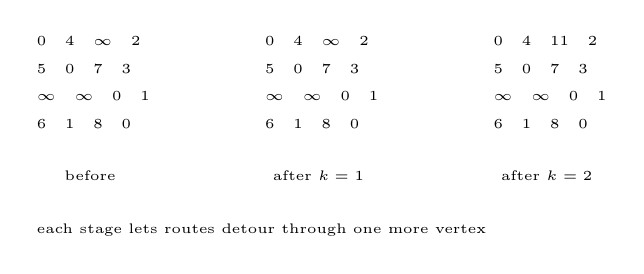
\begin{tikzpicture}[font=\tiny]
\begin{scope}
  \node[anchor=west] at (0,0) {0\quad 4\quad $\infty$\quad 2};
  \node[anchor=west] at (0,-0.35) {5\quad 0\quad 7\quad 3};
  \node[anchor=west] at (0,-0.7) {$\infty$\quad $\infty$\quad 0\quad 1};
  \node[anchor=west] at (0,-1.05) {6\quad 1\quad 8\quad 0};
  \node at (0.8,-1.7) {before};
\end{scope}
\begin{scope}[xshift=2.9cm]
  \node[anchor=west] at (0,0) {0\quad 4\quad $\infty$\quad 2};
  \node[anchor=west] at (0,-0.35) {5\quad 0\quad 7\quad 3};
  \node[anchor=west] at (0,-0.7) {$\infty$\quad $\infty$\quad 0\quad 1};
  \node[anchor=west] at (0,-1.05) {6\quad 1\quad 8\quad 0};
  \node at (0.8,-1.7) {after $k=1$};
\end{scope}
\begin{scope}[xshift=5.8cm]
  \node[anchor=west] at (0,0) {0\quad 4\quad 11\quad 2};
  \node[anchor=west] at (0,-0.35) {5\quad 0\quad 7\quad 3};
  \node[anchor=west] at (0,-0.7) {$\infty$\quad $\infty$\quad 0\quad 1};
  \node[anchor=west] at (0,-1.05) {6\quad 1\quad 8\quad 0};
  \node at (0.8,-1.7) {after $k=2$};
\end{scope}
\node[anchor=west] at (0,-2.4) {each stage lets routes detour through
one more vertex};
\end{tikzpicture}

\caption{The $k$-expansion. Notice each stage only \emph{permits}
detours through one more vertex --- nothing is forced.}
\label{fig:floyd}
\end{figure}

\section{State expansion}\label{sec:state}\index{state expansion}
When the question carries a condition --- a coupon, a ticket, a mode
--- the graph is too small: run shortest paths on
\emph{position $\times$ state}. Vertex $(v, \text{used})$ is a
different vertex from $(v, \text{unused})$.
\begin{example}[CSES \emph{Flight Discount}]\label{ex:discount}
One ticket may be halved.
\par\smallskip
\textbf{Strategy.} Double the graph: coupon-unused layer and spent
layer, with a half-price edge between them. Ordinary Dijkstra on the
expanded graph.
\par\smallskip
\begin{solution}
\lstinputlisting{code/flight_discount.cpp}
Real output (CSES sample):
\begin{lstlisting}[numbers=none]
2
\end{lstlisting}
\end{solution}
\end{example}
\begin{figure}[ht]\centering
% fig39-layers.tex -- Figure 7.11: two-layer expansion for one half-price ticket.
% fstyle.tex -- shared TikZ styles for the figures of this book (palette from lifeos.sty).
\tikzset{%
  cell/.style={draw=ink, minimum width=7mm, minimum height=6.5mm, inner sep=0pt, font=\footnotesize, fill=white},
  cellh/.style={cell, fill=accentsoft, draw=accent},
  cella/.style={cell, fill=amberbg, draw=amber},
  cellg/.style={cell, fill=goodbg, draw=good},
  cellx/.style={cell, fill=graybg, draw=slate, text=slate},
  vtx/.style={circle, draw=ink, minimum size=6.5mm, inner sep=0pt, font=\footnotesize, fill=white},
  vtxh/.style={vtx, draw=accent, fill=accentsoft},
  vtxa/.style={vtx, draw=amber, fill=amberbg},
  vtxg/.style={vtx, draw=good, fill=goodbg},
  vtxd/.style={vtx, draw=slate, fill=graybg, text=slate},
  lab/.style={font=\footnotesize, text=slate},
  labA/.style={font=\footnotesize, text=accent},
  labM/.style={font=\footnotesize, text=amber},
  idx/.style={font=\tiny, text=slate},
  arr/.style={-{stealth}, thick, ink},
  arrA/.style={-{stealth}, thick, accent},
  arrM/.style={-{stealth}, thick, amber},
  arrG/.style={-{stealth}, thick, good},
  edge/.style={thick, ink},
  edgeA/.style={thick, accent},
  edgeM/.style={thick, amber},
}%
% \cellrow{prefix}{x0}{y}{style}{v0,v1,...}: a row of cells named prefix0, prefix1, ... (pitch 0.75cm)
\providecommand{\cellrow}[5]{\foreach \v [count=\i from 0] in {#5} {\node[#4] (#1\i) at (#2+\i*0.75,#3) {\v};}}%
% \cellidx{prefix}{n}{start}: index labels under cells prefix0 .. prefix(n-1)
\providecommand{\cellidx}[3]{\foreach \i in {0,...,\numexpr#2-1\relax} {\node[idx, below=0pt of #1\i] {\the\numexpr\i+#3\relax};}}%
% \fitfig{<tikzpicture>}: shrink the picture to \linewidth only when it would overflow.
\ifdefined\fitbox\else\newsavebox{\fitbox}\fi%
\providecommand{\fitfig}[1]{\sbox{\fitbox}{#1}\ifdim\wd\fitbox>\linewidth\resizebox{\linewidth}{!}{\usebox{\fitbox}}\else\usebox{\fitbox}\fi}%

\begin{tikzpicture}[font=\footnotesize]
\node[vtx, minimum size=8mm] (a0) at (0,1.6) {$A$}; \node[vtx, minimum size=8mm] (b0) at (3.2,1.6) {$B$};
\node[vtxd, minimum size=8mm] (a1) at (0,-0.4) {$A'$}; \node[vtxd, minimum size=8mm] (b1) at (3.2,-0.4) {$B'$};
\draw[arr] (a0) -- (b0) node[midway, above, lab] {$w$};
\draw[arr] (a1) -- (b1) node[midway, below, lab] {$w$};
\draw[arrM] (a0) -- (b1) node[pos=0.28, above right=-1pt, labM, fill=white, inner sep=1pt] {$\lfloor w/2\rfloor$};
\node[lab, anchor=west, align=left] at (4.3,1.6) {upper layer: coupon unused};
\node[lab, anchor=west, align=left] at (4.3,-0.4) {lower layer: coupon spent};
\node[lab, anchor=west, text=amber, align=left] at (4.3,0.6) {discount edge: drops a layer only};
\end{tikzpicture}

\caption{The two-layer expansion. Notice the discount edge only
descends --- the coupon can't be unspent.}
\label{fig:layers}
\end{figure}
\begin{example}[USACO-G \emph{Why Did the Cow Cross the Road}]\label{ex:cow}
Crossing into a different label consumes a ticket; each ticket covers
three crossings.
\par\smallskip
\textbf{Strategy.} The budget is a state: $(r,c,k)$ with $k$ the
crossings used on the current ticket. Same-label moves keep $k$;
boundary moves increment it; the third crossing pays the toll.
\par\smallskip
\begin{solution}
\lstinputlisting{code/cowroad.cpp}
Real output (3$\times$3 demo, $T{=}3$):
\begin{lstlisting}[numbers=none]
4
\end{lstlisting}
\end{solution}
\end{example}
A final named variant: \emph{0-1 BFS}\index{0-1 BFS} --- weights in
$\{0,1\}$ only --- replaces the heap with a deque pushing weight-0
edges to the front.

\begin{exercise}[easy]\label{exr:order}
Does relaxation order matter for Dijkstra's correctness? For
Bellman--Ford's round count?
\end{exercise}
\begin{exercise}[medium]\label{exr:earlyexit}
Bellman--Ford may exit early when a round improves nothing. Show the
early exit can never fire while a reachable negative cycle still has
improvable vertices.
\end{exercise}
\begin{exercise}[medium]\label{exr:whypq}
Why a priority queue and not repeated scans for the minimum?
Estimate both costs on $V{=}10^5$, $E{=}2\cdot10^5$.
\end{exercise}
\begin{exercise}[medium]\label{exr:spotstate}
Name the state for: ``shortest route with at most $k$ road changes''
and ``arriving by exactly time $T$ counts differently than late.''
\end{exercise}

\section{Chapter summary}
\begin{table}[ht]\centering
{\small
\begin{tabularx}{\linewidth}{@{}lYYY@{}}
\toprule
\tablehead\thead{Weights} & \thead{Algorithm} & \thead{Cost} & \thead{Also gives}\\
\midrule
unweighted & BFS & $O(V{+}E)$ & layers\\
non-negative & Dijkstra & $O(E\log V)$ & settled order\\
any (incl.\ neg.) & Bellman--Ford & $O(VE)$ & negative cycles\\
all pairs & Floyd--Warshall & $O(V^3)$ & \texttt{next} paths\\
0/1 only & 0-1 BFS & $O(V{+}E)$ & deque order\\
with a condition & expanded graph & $\times$ states & coupon semantics\\
\bottomrule
\end{tabularx}}
\caption{Pick by the weight law and the shape of the question ---
one source, all pairs, or a condition to fold in.}
\label{tab:sp}
\end{table}

\section{Common mistakes}
\index{common mistakes}
\begin{itemize}
\item \textbf{Dijkstra on negative edges.} The settled set is final
--- one negative edge invalidates the permanence and the algorithm
has no repair path.
\item \textbf{Seeding Bellman--Ford from one source when any cycle
counts.} Only reachable-from-$s$ cycles surface; seed 0 everywhere to
catch all.
\item \textbf{Floyd with $k$ inside.} Loop order \emph{is} the
invariant: $k$ outermost, or intermediate vertices may be reused
illegally.
\item \textbf{Deleting queue entries.} Decrease-key is awkward ---
push a better entry and skip stale pops instead.
\item \textbf{Forgetting \texttt{dist[u]}+w can overflow.} Guard
$\texttt{dist[u]} < \texttt{INF}/2$ before adding to avoid wrapping
past unreachable vertices.
\end{itemize}

\section{Additional exercises}
\begin{exercise}[easy] CSES \emph{Shortest Routes I}. \end{exercise}
\begin{exercise}[easy] CSES \emph{Shortest Routes II}. \end{exercise}
\begin{exercise}[easy] USACO-S \emph{Milk Pails} --- BFS on (x,y) fill states. \end{exercise}
\begin{exercise}[medium] CSES \emph{Flight Discount}. \end{exercise}
\begin{exercise}[medium] CSES \emph{Flight Routes} --- $k$ shortest. \end{exercise}
\begin{exercise}[medium] CSES \emph{Investigation} --- count min paths. \end{exercise}
\begin{exercise}[medium] USACO-G \emph{Milk Pumping} --- Dijkstra + max-flow constraint. \end{exercise}
\begin{exercise}[medium] USACO-G \emph{Shortcut} --- tree + shortcut edges. \end{exercise}
\begin{exercise}[hard] CSES \emph{High Score} --- negative cycle on positive edge. \end{exercise}
\begin{exercise}[hard] CSES \emph{Cycle Finding} --- the reconstruction, coded. \end{exercise}
\begin{exercise}[hard] USACO-G \emph{Lasers and Mirrors} --- direction-state BFS. \end{exercise}
\begin{exercise}[hard] USACO-G \emph{A Pie for a Pie} --- two-shelf trade graph. \end{exercise}
\begin{exercise}[hard] USACO-G \emph{Telephone} --- breed-count state Dijkstra. \end{exercise}

\chapternotes
Relaxation-first framing and the cut argument follow
Laaksonen~\cite{laaksonen2024} and Sannemo~\cite{sannemo2025};
state expansion and the coupon/layer trick are standard in the USACO
Guide's Gold modules~\cite{usacoguide} and
cp-algorithms~\cite{cpalgorithms}; 0-1 BFS and the negative-edge
autopsy appear in Halim~\cite{halimcp4}; archive problems are
official CSES/USACO~\cite{cses}.

\chapter{Disjoint sets and spanning trees}\label{ch:dsu}
\index{disjoint set union}\index{DSU}\index{minimum spanning tree}

Two questions dominate this chapter: are these vertices connected,
and which edges are worth keeping? The disjoint-set union answers the
first in nearly constant time per operation; the minimum spanning
tree answers the second, and the cut property is the single theorem
that makes every MST algorithm correct. After this chapter you will
write a DSU blindfolded, argue Kruskal and Prim from the same
exchange proof, and spot when an offline replay turns ``delete''
into ``insert'' --- the trick that makes deletion queries solvable at
all.

\section{The connectivity problem}\label{sec:conn}\index{connectivity}
Maintain ``are $a$ and $b$ in the same component?'' under edge
insertions. Online algorithms must answer as each query arrives;
offline algorithms see the whole sequence first --- and offline is
where hard problems soften: deleting an edge sequence replayed
backwards is insertion, and DSU handles insertion natively.

\section{The forest representation}\label{sec:forest}
Each set is a rooted tree; \texttt{p[v]} points up. \texttt{find}
walks to the root, \emph{path compression} re-roots the walk's
vertices at the root; \texttt{unite} hangs the smaller root under the
larger (\emph{union by size}). Each half is optional; together they
are nearly free.
\begin{figure}[ht]\centering
% fig40-compress.tex -- Figure 8.1: find(d) with path compression.
% fstyle.tex -- shared TikZ styles for the figures of this book (palette from lifeos.sty).
\tikzset{%
  cell/.style={draw=ink, minimum width=7mm, minimum height=6.5mm, inner sep=0pt, font=\footnotesize, fill=white},
  cellh/.style={cell, fill=accentsoft, draw=accent},
  cella/.style={cell, fill=amberbg, draw=amber},
  cellg/.style={cell, fill=goodbg, draw=good},
  cellx/.style={cell, fill=graybg, draw=slate, text=slate},
  vtx/.style={circle, draw=ink, minimum size=6.5mm, inner sep=0pt, font=\footnotesize, fill=white},
  vtxh/.style={vtx, draw=accent, fill=accentsoft},
  vtxa/.style={vtx, draw=amber, fill=amberbg},
  vtxg/.style={vtx, draw=good, fill=goodbg},
  vtxd/.style={vtx, draw=slate, fill=graybg, text=slate},
  lab/.style={font=\footnotesize, text=slate},
  labA/.style={font=\footnotesize, text=accent},
  labM/.style={font=\footnotesize, text=amber},
  idx/.style={font=\tiny, text=slate},
  arr/.style={-{stealth}, thick, ink},
  arrA/.style={-{stealth}, thick, accent},
  arrM/.style={-{stealth}, thick, amber},
  arrG/.style={-{stealth}, thick, good},
  edge/.style={thick, ink},
  edgeA/.style={thick, accent},
  edgeM/.style={thick, amber},
}%
% \cellrow{prefix}{x0}{y}{style}{v0,v1,...}: a row of cells named prefix0, prefix1, ... (pitch 0.75cm)
\providecommand{\cellrow}[5]{\foreach \v [count=\i from 0] in {#5} {\node[#4] (#1\i) at (#2+\i*0.75,#3) {\v};}}%
% \cellidx{prefix}{n}{start}: index labels under cells prefix0 .. prefix(n-1)
\providecommand{\cellidx}[3]{\foreach \i in {0,...,\numexpr#2-1\relax} {\node[idx, below=0pt of #1\i] {\the\numexpr\i+#3\relax};}}%
% \fitfig{<tikzpicture>}: shrink the picture to \linewidth only when it would overflow.
\ifdefined\fitbox\else\newsavebox{\fitbox}\fi%
\providecommand{\fitfig}[1]{\sbox{\fitbox}{#1}\ifdim\wd\fitbox>\linewidth\resizebox{\linewidth}{!}{\usebox{\fitbox}}\else\usebox{\fitbox}\fi}%

\begin{tikzpicture}[font=\footnotesize]
% before
\node[vtx] (r) at (0,3.0) {r}; \node[vtx] (a) at (0,2.1) {a}; \node[vtxh] (b) at (0,1.2) {b}; \node[vtxh] (c) at (0,0.3) {c};
\node[vtxh] (d) at (0,-0.6) {d}; \node[vtx] (x) at (1.1,0.3) {x};
\draw[arr, shorten >=1pt] (a)--(r); \draw[arr, shorten >=1pt] (b)--(a); \draw[arr, shorten >=1pt] (c)--(b); \draw[arr, shorten >=1pt] (d)--(c); \draw[arr, shorten >=1pt] (x)--(b);
\node[lab, align=center] at (0.5,-1.5) {before \texttt{find(d)}};
\draw[arrA, ultra thick] (2.2,1.2) -- (3.2,1.2) node[midway, above, labA] {find};
% after
\node[vtx] (r2) at (5.5,3.0) {r};
\node[vtx] (a2) at (4.3,1.7) {a}; \node[vtxh] (b2) at (5.1,1.7) {b}; \node[vtxh] (c2) at (5.9,1.7) {c}; \node[vtxh] (d2) at (6.7,1.7) {d};
\node[vtx] (x2) at (5.1,0.3) {x};
\foreach \n in {a2,b2,c2,d2} \draw[arr, shorten >=1pt] (\n)--(r2);
\draw[arr, shorten >=1pt] (x2)--(b2);
\node[lab, align=center] at (5.5,-0.55) {after: path re-parented to the root,\\ off-path $x$ untouched};
\end{tikzpicture}

\caption{The same find, before and after. Notice compression only
re-parents vertices on the walked path --- others keep their depth
until their turn.}
\label{fig:compress}
\end{figure}
\begin{figure}[ht]\centering
\begin{tikzpicture}[font=\footnotesize]
\begin{scope}
\node[circle,draw=slate,fill=accentsoft,font=\tiny] at (0,1) {big};
\node[circle,draw=slate,font=\tiny] at (0.8,1) {small};
\draw[-{stealth},amber,thick] (0.8,1) to[out=45,in=45] (0,1);
\node[font=\tiny] at (0.4,0.4) {small $\to$ big: stays shallow};
\end{scope}
\begin{scope}[xshift=4.4cm]
\node[circle,draw=slate,font=\tiny] at (0,1) {big};
\node[circle,draw=slate,fill=accentsoft,font=\tiny] at (0.8,1) {small};
\draw[-{stealth},amber,thick,dashed] (0,1) to[out=135,in=135] (0.8,1);
\node[font=\tiny] at (0.4,0.4) {big $\to$ small: deepens};
\end{scope}
\end{tikzpicture}

\caption{Union by size. Notice the asymmetry: only hanging the larger
under the smaller deepens anything; the other direction never adds
depth.}
\label{fig:unionsize}
\end{figure}
\begin{lstlisting}[language=C++,caption={\texttt{dsu.h}: path
halving + union by size + component sizes.},label={lst:dsu}]
\end{lstlisting}
\lstinputlisting{code/dsu.h}

\section{The amortized bound}\label{sec:ack}
With both optimizations, $m$ operations cost $O(m\,\alpha(n))$ where
$\alpha$ is the inverse Ackermann function --- bounded by 4 for any
$n$ in this universe. The proof charges each pointer hop to a rank
increase budget; sketch only: ranks are potential, compression spends
it. In contest terms: treat each operation as $O(1)$.

\section{The cut property}\label{sec:cut}\index{cut property}
For any cut $(S, V\setminus S)$, the lightest crossing edge belongs
to \emph{some} MST. Proof by exchange: take an MST using a heavier
crossing edge $f$; swapping in the light edge $e$ keeps a spanning
tree and only lowers the cost. Every MST algorithm is this theorem in
a different costume.
\begin{figure}[ht]\centering
% fig42-cutprop.tex -- Figure 8.3: the cut property; the lightest edge crossing a cut belongs to some MST.
% fstyle.tex -- shared TikZ styles for the figures of this book (palette from lifeos.sty).
\tikzset{%
  cell/.style={draw=ink, minimum width=7mm, minimum height=6.5mm, inner sep=0pt, font=\footnotesize, fill=white},
  cellh/.style={cell, fill=accentsoft, draw=accent},
  cella/.style={cell, fill=amberbg, draw=amber},
  cellg/.style={cell, fill=goodbg, draw=good},
  cellx/.style={cell, fill=graybg, draw=slate, text=slate},
  vtx/.style={circle, draw=ink, minimum size=6.5mm, inner sep=0pt, font=\footnotesize, fill=white},
  vtxh/.style={vtx, draw=accent, fill=accentsoft},
  vtxa/.style={vtx, draw=amber, fill=amberbg},
  vtxg/.style={vtx, draw=good, fill=goodbg},
  vtxd/.style={vtx, draw=slate, fill=graybg, text=slate},
  lab/.style={font=\footnotesize, text=slate},
  labA/.style={font=\footnotesize, text=accent},
  labM/.style={font=\footnotesize, text=amber},
  idx/.style={font=\tiny, text=slate},
  arr/.style={-{stealth}, thick, ink},
  arrA/.style={-{stealth}, thick, accent},
  arrM/.style={-{stealth}, thick, amber},
  arrG/.style={-{stealth}, thick, good},
  edge/.style={thick, ink},
  edgeA/.style={thick, accent},
  edgeM/.style={thick, amber},
}%
% \cellrow{prefix}{x0}{y}{style}{v0,v1,...}: a row of cells named prefix0, prefix1, ... (pitch 0.75cm)
\providecommand{\cellrow}[5]{\foreach \v [count=\i from 0] in {#5} {\node[#4] (#1\i) at (#2+\i*0.75,#3) {\v};}}%
% \cellidx{prefix}{n}{start}: index labels under cells prefix0 .. prefix(n-1)
\providecommand{\cellidx}[3]{\foreach \i in {0,...,\numexpr#2-1\relax} {\node[idx, below=0pt of #1\i] {\the\numexpr\i+#3\relax};}}%
% \fitfig{<tikzpicture>}: shrink the picture to \linewidth only when it would overflow.
\ifdefined\fitbox\else\newsavebox{\fitbox}\fi%
\providecommand{\fitfig}[1]{\sbox{\fitbox}{#1}\ifdim\wd\fitbox>\linewidth\resizebox{\linewidth}{!}{\usebox{\fitbox}}\else\usebox{\fitbox}\fi}%

\begin{tikzpicture}[font=\footnotesize]
\draw[rounded corners=8pt, draw=accent, fill=accentsoft] (-0.2,-0.2) rectangle (3.4,3.6);
\draw[rounded corners=8pt, draw=amber, fill=amberbg] (5.2,-0.2) rectangle (8.8,3.6);
\node[labA] at (1.6,3.9) {$S$}; \node[labM] at (7.0,3.9) {$V\setminus S$};
\node[vtx] (p1) at (0.8,2.8) {}; \node[vtx] (p2) at (2.4,2.6) {}; \node[vtx] (p3) at (1.2,0.9) {}; \node[vtx] (p4) at (2.6,0.6) {};
\node[vtx] (q1) at (6.0,2.7) {}; \node[vtx] (q2) at (7.8,2.9) {}; \node[vtx] (q3) at (6.2,0.8) {}; \node[vtx] (q4) at (7.9,0.8) {};
\draw[edge, slate] (p1)--(p2) (p1)--(p3) (p3)--(p4) (q1)--(q2) (q1)--(q3) (q3)--(q4);
\draw[edge, slate] (p2) -- (q1) node[midway, above, lab] {9};
\draw[edgeM, very thick] (p4) -- (q3) node[midway, below, labM] {3};
\draw[edge, slate] (p2) -- (q4) node[pos=0.25, below left=1pt, lab] {6};
\node[labM, align=center] at (4.0,-1.0) {lightest crossing edge (3): safe to take};
\draw[dashed, slate] (4.0,-0.4) -- (4.0,3.9);
\end{tikzpicture}

\caption{The cut property. Notice nothing depends on which MST you
started from --- exchange against \emph{any} of them.}
\label{fig:cutprop}
\end{figure}

\section{Kruskal}\label{sec:kruskal}\index{Kruskal}
Sort edges, accept those joining different components. Each accepted
edge is the lightest crossing of the cut between the two components
--- the cut property again, applied greedily. Cost: sorting
dominates, $O(E\log E)$.
\begin{lstlisting}[language=C++,caption={\texttt{kruskal.h} on top of
\texttt{DSU}.},label={lst:kruskal}]
\end{lstlisting}
\lstinputlisting{code/kruskal.h}
\begin{example}[CSES \emph{Road Reparation}]\label{ex:reparation}
Cheapest way to reconnect the cities.
\par\smallskip
\textbf{Strategy.} ``Cheapest connection covering all'' is an MST;
a leftover of fewer than $n{-}1$ accepted edges means the graph was
never connected.
\par\smallskip
\begin{solution}
\lstinputlisting{code/road_reparation.cpp}
Real output (CSES sample):
\begin{lstlisting}[numbers=none]
14
\end{lstlisting}
\end{solution}
\end{example}
\begin{figure}[ht]\centering
% fig43-kruskal.tex -- Figure 8.4: Kruskal on the CSES Road Reparation sample (answer 14).
% fstyle.tex -- shared TikZ styles for the figures of this book (palette from lifeos.sty).
\tikzset{%
  cell/.style={draw=ink, minimum width=7mm, minimum height=6.5mm, inner sep=0pt, font=\footnotesize, fill=white},
  cellh/.style={cell, fill=accentsoft, draw=accent},
  cella/.style={cell, fill=amberbg, draw=amber},
  cellg/.style={cell, fill=goodbg, draw=good},
  cellx/.style={cell, fill=graybg, draw=slate, text=slate},
  vtx/.style={circle, draw=ink, minimum size=6.5mm, inner sep=0pt, font=\footnotesize, fill=white},
  vtxh/.style={vtx, draw=accent, fill=accentsoft},
  vtxa/.style={vtx, draw=amber, fill=amberbg},
  vtxg/.style={vtx, draw=good, fill=goodbg},
  vtxd/.style={vtx, draw=slate, fill=graybg, text=slate},
  lab/.style={font=\footnotesize, text=slate},
  labA/.style={font=\footnotesize, text=accent},
  labM/.style={font=\footnotesize, text=amber},
  idx/.style={font=\tiny, text=slate},
  arr/.style={-{stealth}, thick, ink},
  arrA/.style={-{stealth}, thick, accent},
  arrM/.style={-{stealth}, thick, amber},
  arrG/.style={-{stealth}, thick, good},
  edge/.style={thick, ink},
  edgeA/.style={thick, accent},
  edgeM/.style={thick, amber},
}%
% \cellrow{prefix}{x0}{y}{style}{v0,v1,...}: a row of cells named prefix0, prefix1, ... (pitch 0.75cm)
\providecommand{\cellrow}[5]{\foreach \v [count=\i from 0] in {#5} {\node[#4] (#1\i) at (#2+\i*0.75,#3) {\v};}}%
% \cellidx{prefix}{n}{start}: index labels under cells prefix0 .. prefix(n-1)
\providecommand{\cellidx}[3]{\foreach \i in {0,...,\numexpr#2-1\relax} {\node[idx, below=0pt of #1\i] {\the\numexpr\i+#3\relax};}}%
% \fitfig{<tikzpicture>}: shrink the picture to \linewidth only when it would overflow.
\ifdefined\fitbox\else\newsavebox{\fitbox}\fi%
\providecommand{\fitfig}[1]{\sbox{\fitbox}{#1}\ifdim\wd\fitbox>\linewidth\resizebox{\linewidth}{!}{\usebox{\fitbox}}\else\usebox{\fitbox}\fi}%

\begin{tikzpicture}[font=\footnotesize]
\node[vtx] (n1) at (0,2) {1}; \node[vtx] (n2) at (2.2,2) {2}; \node[vtx] (n3) at (4.4,2) {3};
\node[vtx] (n5) at (0,0) {5}; \node[vtx] (n4) at (2.2,0) {4};
\draw[edge, slate, dashed] (n1)--(n5) node[midway, left, lab] {7};
\draw[edge, slate, dashed] (n3)--(n4) node[midway, below right, lab] {8};
\draw[edgeM, very thick] (n1)--(n2) node[midway, above, labM] {3};
\draw[edgeM, very thick] (n2)--(n3) node[midway, above, labM] {5};
\draw[edgeM, very thick] (n2)--(n4) node[midway, right, labM] {2};
\draw[edgeM, very thick] (n5)--(n4) node[midway, below, labM] {4};
\node[lab, align=left, anchor=west] at (5.6,2.35) {edges sorted by weight:};
\foreach \y/\w/\e/\verdict in {1.7/2/{2--4}/{accept}, 1.2/3/{1--2}/{accept}, 0.7/4/{4--5}/{accept}, 0.2/5/{2--3}/{accept}, -0.3/7/{1--5}/{skip (same set)}, -0.8/8/{3--4}/{skip (same set)}}
  \node[lab, anchor=west] at (5.6,\y) {$\w$: edge \e\ $\to$ \verdict};
\node[labM] at (7.4,-1.5) {total $2+3+4+5=14$};
\end{tikzpicture}

\caption{Kruskal's accept/skip rhythm. Notice the skipped edge is
rejected \emph{because} its endpoints already merged --- the DSU is
the algorithm's memory.}
\label{fig:kruskal}
\end{figure}

\section{Prim}\label{sec:prim}\index{Prim}
Grow one tree: a priority queue holds frontier edges; pop the
lightest, settle its far vertex, push its edges. It is Dijkstra's
skeleton with edge weight instead of distance --- and wins when the
graph is dense enough that sorting all edges is the bottleneck.
\begin{lstlisting}[language=C++,caption={\texttt{prim.h}: the pq
frontier.},label={lst:prim}]
\end{lstlisting}
\lstinputlisting{code/prim.h}

\section{Worked examples}
\begin{example}[CSES \emph{Road Construction}]\label{ex:constr}
After each new road: component count, largest component.
\par\smallskip
\textbf{Strategy.} Both answers live in the DSU's size array:
merges decrement the count and grow one component.
\par\smallskip
\begin{solution}
\lstinputlisting{code/road_construction.cpp}
Real output (CSES sample):
\begin{lstlisting}[numbers=none]
4 2
3 3
2 3
\end{lstlisting}
\end{solution}
\end{example}
\begin{example}[CSES \emph{Building Roads}]\label{ex:roads}
Minimum roads to connect all cities, then print them.
\par\smallskip
\textbf{Strategy.} Components minus one is the count; linking
component roots in a chain realizes it.
\par\smallskip
\begin{solution}
\lstinputlisting{code/building_roads.cpp}
Real output (CSES sample):
\begin{lstlisting}[numbers=none]
1
1 3
\end{lstlisting}
\end{solution}
\end{example}
\begin{example}[USACO-S \emph{Closing the Farm}]\label{ex:farm}
After each barn closes, is the farm still fully connected?
\par\smallskip
\textbf{Strategy.} DSU cannot delete --- so run time backwards:
start from the last surviving barn and \emph{insert} barns in reverse
order, recording the connectivity of each state \emph{before}
the closed barn is re-inserted (the answer asks for the state
\emph{after} that closing; an empty remainder is vacuously
connected)
(Figure~\ref{fig:farmtime}).
\par\smallskip
\begin{solution}
\lstinputlisting{code/closing_farm.cpp}
Real output (4-barn star, all states connected):
\begin{lstlisting}[numbers=none]
YES
YES
YES
YES
\end{lstlisting}
\end{solution}
\end{example}
\begin{figure}[ht]\centering
\begin{tikzpicture}[font=\footnotesize]
\node[font=\tiny] at (0,0.5) {delete 4, 3, 1, 2};
\draw[-{stealth},slate] (0,0.2)--(2.6,0.2);
\node[font=\tiny] at (3.4,0.2) {time};
\begin{scope}[yshift=-0.7cm]
\node[font=\tiny] at (0,0.3) {add 2, 1, 3, 4};
\draw[-{stealth},amber,thick] (2.6,-0.1)--(0,-0.1);
\node[font=\tiny] at (3.4,0) {replay};
\end{scope}
\node[font=\tiny,align=center] at (1.3,-1.4) {offline: answer each prefix\\after re-adding in reverse};
\end{tikzpicture}

\caption{The timeline reversal. Notice the forward question and the
backward algorithm share \emph{the same states} --- replaying
backwards visits every intermediate farm the original run did.}
\label{fig:farmtime}
\end{figure}

\begin{exercise}[easy]\label{exr:fu}
In \texttt{unite(a,b)}, which order runs \texttt{find} first --- and
why does union-by-size need the \emph{root} sizes, not arbitrary
sizes?
\end{exercise}
\begin{exercise}[medium]\label{exr:whichcut}
Kruskal's next accepted edge $e$ between components $A,B$: exhibit
the cut whose light edge $e$ is, and conclude its membership.
\end{exercise}
\begin{exercise}[medium]\label{exr:reverse}
Give a query sequence where offline reversal is essential (not just
convenient): name one operation DSU fundamentally cannot undo.
\end{exercise}

\section{Chapter summary}
\begin{table}[ht]\centering
{\small
\begin{tabularx}{\linewidth}{@{}lYYY@{}}
\toprule
\tablehead\thead{Task} & \thead{Tool} & \thead{Cost} & \thead{Watch for}\\
\midrule
connected? + merge & DSU & $\sim O(1)$/op & no deletes\\
all-pairs min tree & Kruskal & $O(E\log E)$ & sort dominates\\
dense-graph MST & Prim & $O(E\log V)$ & pq frontier\\
deletion queries & offline reverse & same ops & replay order\\
\bottomrule
\end{tabularx}}
\caption{One theorem (cut property) under both MST algorithms; one
trick (offline reversal) under every deletion problem.}
\label{tab:dsu}
\end{table}

\section{Common mistakes}
\index{common mistakes}
\begin{itemize}
\item \textbf{Union without \texttt{find}.} \texttt{p[a]=p[b]} links
arbitrary members, not roots --- always unite
\texttt{find(a)},\,\texttt{find(b)}.
\item \textbf{Skipping compression \emph{and} size.} One alone helps;
neither degenerates to $O(n)$ per find --- keep both.
\item \textbf{Trying to delete with DSU.} There is no
\texttt{un-unite}; offline reversal or a different structure is the
answer.
\item \textbf{Assuming MST is unique.} Equal weights admit several;
the cut property promises \emph{some} MST, not \emph{the} MST ---
handle ties deliberately when the problem counts trees.
\item \textbf{Forgetting the disconnected case.} A forest is legal
input --- \texttt{mst.size() < n-1} is the IMPOSSIBLE check.
\end{itemize}

\section{Additional exercises}
\begin{exercise}[easy] CSES \emph{Road Reparation}. \end{exercise}
\begin{exercise}[easy] USACO-S \emph{Closing the Farm}. \end{exercise}
\begin{exercise}[easy] USACO-G \emph{MooTube} --- threshold components. \end{exercise}
\begin{exercise}[medium] USACO-S \emph{Wormhole Sort} --- DSU + binary search. \end{exercise}
\begin{exercise}[medium] USACO-G \emph{Moocast} --- MST-style radii. \end{exercise}
\begin{exercise}[medium] USACO-G \emph{I Would Walk 500 Miles} --- implicit-edge Kruskal. \end{exercise}
\begin{exercise}[medium] CF \emph{Design Tutorial: Inverse the Problem} --- reconstruct from MST. \end{exercise}
\begin{exercise}[hard] CSES \emph{New Roads Queries} --- online MST edge questions. \end{exercise}
\begin{exercise}[hard] USACO-G \emph{Portals} --- MST on portal+cost edges. \end{exercise}
\begin{exercise}[hard] USACO-G \emph{Fenced In} --- boundary-strip Kruskal. \end{exercise}
\begin{exercise}[hard] USACO-OS \emph{Ski Course Rating} --- MST + queries. \end{exercise}
\begin{exercise}[hard] Baltic OI 2016 \emph{Park} --- MST + LCA path max. \end{exercise}

\chapternotes
DSU amortization and the cut-property-first MST treatment follow
Laaksonen~\cite{laaksonen2024} and Sannemo~\cite{sannemo2025}; the
offline-reversal pattern and threshold-component problems are the
USACO Guide's DSU module~\cite{usacoguide}; cp-algorithms carries the
charged-ranks proof sketch and MST variants~\cite{cpalgorithms};
Halim supplies the named variants~\cite{halimcp4}; archive problems
are official CSES/USACO~\cite{cses}.

\chapter{Tree algorithms: subtrees, diameters, LCA}\label{ch:trees}
\index{tree}\index{LCA}\index{binary lifting}\index{rerooting}

A tree is the graph where every question has a canonical answer:
exactly one path between any two vertices, and rooting turns
``around'' into ``down.'' This chapter collects the five patterns
that solve almost every tree problem on the archive: post-order
subtree sums, the two-DFS diameter, rerooting (answers for every
root in one pass), the Euler tour that turns subtrees into subarrays,
and binary lifting for ancestors and LCA. After it you will compute
per-vertex farthest distances, answer distance queries in
$O(\log n)$, and see every ``tree problem'' as pick-a-pattern.

% from-zero:begin
\begin{rulebox}[Before you start]
Chapter~7 (DFS) and Chapter~9 (a tree is a connected graph with no cycle). \emph{Recap:} in a tree there is exactly one simple path between any two vertices, which is why tree problems are easier than general graph problems.
\end{rulebox}
\begin{wins}[After this chapter you can]
\begin{itemize}
\item root a tree and compute subtree sizes, depths and sums with one DFS;
\item find a tree's diameter with two DFS passes;
\item flatten a tree into an array with an Euler tour so range tools apply;
\item answer lowest-common-ancestor and path-distance queries with binary lifting.
\end{itemize}
\end{wins}
\begin{principle}[How to think about this]
A tree is a graph with no loops, so there is exactly one way to get anywhere. That removes most of the difficulty: you can solve a problem for a small subtree and combine the answers upward. The habit to build is ``solve my children first, then combine,'' which is a recursive way of thinking that returns again in dynamic programming.
\end{principle}
% from-zero:end

\section{The shape of a tree}\label{sec:tshape}
$n$ vertices, $n{-}1$ edges, connected, acyclic: any two properties
imply the third. Rooting is a \emph{design choice} --- most
algorithms pick an arbitrary root and exploit ``parent vs children''
as the graph's only direction. Unique paths are what make ancestors,
depths and diameters well-defined.

\section{Subtree aggregates}\label{sec:subtree}\index{subtree aggregate}
Post-order accumulation computes any quantity that depends on
children first: sizes, sums, counts. The pattern is one DFS;
everything else in the chapter builds on it.
\begin{example}[CSES \emph{Subordinates}]\label{ex:subor}
Per employee, count the whole subtree beneath them.
\par\smallskip
\textbf{Strategy.} The hierarchy is already rooted: size(v) =
$\sum_{u\text{ child}}(1+\text{size}(u))$ computed in one post-order
pass.
\par\smallskip
\begin{solution}
\lstinputlisting{code/subordinates.cpp}
Real output (CSES sample):
\begin{lstlisting}[numbers=none]
4 0 2 0 0
\end{lstlisting}
\end{solution}
\end{example}

\section{Diameter: two DFS}\label{sec:diam}\index{diameter}
The farthest vertex from \emph{any} start is a diameter endpoint;
a second farthest-search from it finds the other end. Proof sketch:
let $u,v$ be a diameter and $a$ the farthest vertex from start $s$;
if $a$ were not an endpoint, a path past $u$ or $v$ would beat
$a$'s distance --- contradiction. (The common wrong proof --- ``it
works because it works on paths'' --- is flagged in the mistakes.)
\begin{example}[CSES \emph{Tree Diameter}]\label{ex:diam}
Longest path in the tree.
\par\smallskip
\textbf{Strategy.} Two searches, no DP: farthest-from-1, then
farthest-from-that.
\par\smallskip
\begin{solution}
\lstinputlisting{code/tree_diameter.cpp}
Real output (CSES sample):
\begin{lstlisting}[numbers=none]
3
\end{lstlisting}
\end{solution}
\end{example}
\begin{figure}[ht]\centering
% fig47-twodfs.tex -- Figure 10.x: two-DFS diameter. Path u1-u2-u3-u4-u5 plus leaf a on u2.
% fstyle.tex -- shared TikZ styles for the figures of this book (palette from lifeos.sty).
\tikzset{%
  cell/.style={draw=ink, minimum width=7mm, minimum height=6.5mm, inner sep=0pt, font=\footnotesize, fill=white},
  cellh/.style={cell, fill=accentsoft, draw=accent},
  cella/.style={cell, fill=amberbg, draw=amber},
  cellg/.style={cell, fill=goodbg, draw=good},
  cellx/.style={cell, fill=graybg, draw=slate, text=slate},
  vtx/.style={circle, draw=ink, minimum size=6.5mm, inner sep=0pt, font=\footnotesize, fill=white},
  vtxh/.style={vtx, draw=accent, fill=accentsoft},
  vtxa/.style={vtx, draw=amber, fill=amberbg},
  vtxg/.style={vtx, draw=good, fill=goodbg},
  vtxd/.style={vtx, draw=slate, fill=graybg, text=slate},
  lab/.style={font=\footnotesize, text=slate},
  labA/.style={font=\footnotesize, text=accent},
  labM/.style={font=\footnotesize, text=amber},
  idx/.style={font=\tiny, text=slate},
  arr/.style={-{stealth}, thick, ink},
  arrA/.style={-{stealth}, thick, accent},
  arrM/.style={-{stealth}, thick, amber},
  arrG/.style={-{stealth}, thick, good},
  edge/.style={thick, ink},
  edgeA/.style={thick, accent},
  edgeM/.style={thick, amber},
}%
% \cellrow{prefix}{x0}{y}{style}{v0,v1,...}: a row of cells named prefix0, prefix1, ... (pitch 0.75cm)
\providecommand{\cellrow}[5]{\foreach \v [count=\i from 0] in {#5} {\node[#4] (#1\i) at (#2+\i*0.75,#3) {\v};}}%
% \cellidx{prefix}{n}{start}: index labels under cells prefix0 .. prefix(n-1)
\providecommand{\cellidx}[3]{\foreach \i in {0,...,\numexpr#2-1\relax} {\node[idx, below=0pt of #1\i] {\the\numexpr\i+#3\relax};}}%
% \fitfig{<tikzpicture>}: shrink the picture to \linewidth only when it would overflow.
\ifdefined\fitbox\else\newsavebox{\fitbox}\fi%
\providecommand{\fitfig}[1]{\sbox{\fitbox}{#1}\ifdim\wd\fitbox>\linewidth\resizebox{\linewidth}{!}{\usebox{\fitbox}}\else\usebox{\fitbox}\fi}%

\begin{tikzpicture}[font=\footnotesize]
\foreach \i in {1,...,5} \node[vtx] (u\i) at (\i*1.6,0) {$u_\i$};
\node[vtxh] (a) at (3.2,1.4) {$a$};
\draw[edge] (u1)--(u2)--(u3)--(u4)--(u5) (a)--(u2);
\node[vtxa, minimum size=6.5mm] at (u5) {$u_5$};
\draw[edgeM, very thick] (a)--(u2)--(u3)--(u4)--(u5);
\draw[edgeA, very thick, dashed, transform canvas={yshift=-3pt}] (u5)--(u4)--(u3)--(u2)--(u1);
\node[labM, anchor=west] at (0.7,-1.0) {1st DFS from $a$ (amber path): farthest vertex is $u_5$, distance $4$};
\node[labA, anchor=west] at (0.7,-1.6) {2nd DFS from $u_5$ (blue dashes): farthest is $u_1$, distance $4$ $=$ the diameter};
\end{tikzpicture}

\caption{The farthest-point argument. Notice the claim is about
endpoints, not the path --- endpoint first, distance second.}
\label{fig:twodfs}
\end{figure}

\section{Rerooting}\label{sec:reroot}\index{rerooting}
``For every root'' doubles the work naively; rerooting does it in
two passes: \texttt{down[v]} from children, then \texttt{up[v]}
passed down from parent using each child's best \emph{sibling}
value. Per vertex the answer combines both.
\begin{example}[CSES \emph{Tree Distances II}]\label{ex:dist2}
Each vertex's farthest distance.
\par\smallskip
\textbf{Strategy.} The answer is $\max(\texttt{down},\texttt{up})$;
the sibling-max trick supplies each child's ``up'' in $O(\deg v)$.
\par\smallskip
\begin{solution}
\lstinputlisting{code/tree_distances2.cpp}
Real output (CSES sample):
\begin{lstlisting}[numbers=none]
2 3 2 3 3
\end{lstlisting}
\end{solution}
\end{example}
\begin{figure}[ht]\centering
% fig48-reroot.tex -- Figure 10.x: rerooting; up[u] = 1 + max(up[v], 1 + down[w]) for sibling w. Here up[v]=1, down[w]=2.
% fstyle.tex -- shared TikZ styles for the figures of this book (palette from lifeos.sty).
\tikzset{%
  cell/.style={draw=ink, minimum width=7mm, minimum height=6.5mm, inner sep=0pt, font=\footnotesize, fill=white},
  cellh/.style={cell, fill=accentsoft, draw=accent},
  cella/.style={cell, fill=amberbg, draw=amber},
  cellg/.style={cell, fill=goodbg, draw=good},
  cellx/.style={cell, fill=graybg, draw=slate, text=slate},
  vtx/.style={circle, draw=ink, minimum size=6.5mm, inner sep=0pt, font=\footnotesize, fill=white},
  vtxh/.style={vtx, draw=accent, fill=accentsoft},
  vtxa/.style={vtx, draw=amber, fill=amberbg},
  vtxg/.style={vtx, draw=good, fill=goodbg},
  vtxd/.style={vtx, draw=slate, fill=graybg, text=slate},
  lab/.style={font=\footnotesize, text=slate},
  labA/.style={font=\footnotesize, text=accent},
  labM/.style={font=\footnotesize, text=amber},
  idx/.style={font=\tiny, text=slate},
  arr/.style={-{stealth}, thick, ink},
  arrA/.style={-{stealth}, thick, accent},
  arrM/.style={-{stealth}, thick, amber},
  arrG/.style={-{stealth}, thick, good},
  edge/.style={thick, ink},
  edgeA/.style={thick, accent},
  edgeM/.style={thick, amber},
}%
% \cellrow{prefix}{x0}{y}{style}{v0,v1,...}: a row of cells named prefix0, prefix1, ... (pitch 0.75cm)
\providecommand{\cellrow}[5]{\foreach \v [count=\i from 0] in {#5} {\node[#4] (#1\i) at (#2+\i*0.75,#3) {\v};}}%
% \cellidx{prefix}{n}{start}: index labels under cells prefix0 .. prefix(n-1)
\providecommand{\cellidx}[3]{\foreach \i in {0,...,\numexpr#2-1\relax} {\node[idx, below=0pt of #1\i] {\the\numexpr\i+#3\relax};}}%
% \fitfig{<tikzpicture>}: shrink the picture to \linewidth only when it would overflow.
\ifdefined\fitbox\else\newsavebox{\fitbox}\fi%
\providecommand{\fitfig}[1]{\sbox{\fitbox}{#1}\ifdim\wd\fitbox>\linewidth\resizebox{\linewidth}{!}{\usebox{\fitbox}}\else\usebox{\fitbox}\fi}%

\begin{tikzpicture}[font=\footnotesize]
\node[vtx] (p) at (2,3.6) {$p$}; \node[vtx] (v) at (2,2.4) {$v$};
\node[vtxh] (u) at (0.8,1.2) {$u$}; \node[vtx] (w) at (3.2,1.2) {$w$};
\node[vtx] (x) at (3.2,0) {$x$}; \node[vtx] (y) at (3.2,-1.2) {$y$};
\draw[edge] (p)--(v)--(u) (v)--(w)--(x)--(y);
\draw[arrA, bend right=40] (p.west) to node[left, labA] {up$[v]=1$} (v.west);
\draw[arrM, bend left=35, dashed] (w.east) to node[right, labM, align=left] {down$[w]=2$} (y.east);
\node[labM, align=left, anchor=west] at (6.3,1.9) {pass 2: up$[u]$ $=1+\max\big(\mathrm{up}[v],\ 1+\mathrm{down}[w]\big)$};
\node[labM, align=left, anchor=west] at (6.3,1.2) {\phantom{pass 2: up$[u]$ }$=1+\max(1,3)=4$};
\node[lab, align=left, anchor=west, text width=6.2cm] at (6.3,0.2) {the longest path from $u$ goes up to $v$, then down through the \emph{sibling} $w$ to $y$};
\end{tikzpicture}

\caption{What travels down in pass two. Notice a child never sees its
own subtree in its ``up'' value --- the sibling max is the key step.}
\label{fig:reroot}
\end{figure}

\section{The Euler tour}\label{sec:euler}\index{Euler tour}
\texttt{tin[v]} on entry, \texttt{tout[v]} on exit: every subtree
becomes the interval $[\texttt{tin},\texttt{tout})$, turning
``update/query a subtree'' into range operations --- the bridge to
segment trees in Chapter~12.
\begin{figure}[ht]\centering
\begin{tikzpicture}[font=\footnotesize]
\node[circle,draw=slate,font=\tiny] (r) at (2,1.6) {1};
\node[circle,draw=slate,font=\tiny] (a) at (1,0.8) {2};
\node[circle,draw=slate,font=\tiny] (b) at (3,0.8) {3};
\node[circle,draw=slate,font=\tiny] (c) at (1,0) {4};
\draw[slate] (r)--(a) (r)--(b) (a)--(c);
\node[font=\tiny,anchor=west] at (4.2,1.2) {tin: 1=0, 2=1, 4=2, 3=3};
\node[font=\tiny,anchor=west] at (4.2,0.7) {tout: 1=4, 2=3, 4=3, 3=4};
\node[font=\tiny,anchor=west] at (4.2,0.2) {subtree(2) = $[1,3)$: $\{2,4\}$};
\node[font=\tiny] at (2,-0.8) {every subtree is one interval};
\end{tikzpicture}

\caption{Euler intervals nested. Notice containment is interval
containment --- $u$ is in $v$'s subtree iff
$\texttt{tin}[v]\le\texttt{tin}[u]<\texttt{tout}[v]$.}
\label{fig:euler}
\end{figure}

\section{Binary lifting and LCA}\label{sec:lca}\index{binary lifting}
Store the $2^k$-th ancestor of every vertex: $\texttt{up}[k][v] =
\texttt{up}[k{-}1][\texttt{up}[k{-}1][v]]$ --- a doubling table built
in $O(n\log n)$. $k$-th ancestor: follow set bits. LCA: equalize
depth, then lift both ends by descending powers of two until their
parents coincide. (An Euler-tour + sparse-RMQ alternative exists;
lifting is the workhorse.)
\begin{figure}[ht]\centering
\begin{tikzpicture}[font=\footnotesize]
\foreach \i/\v in {0/7,1/5,2/3,3/1}
  \node[circle,draw=slate,font=\tiny] (\v) at (\i*1.1,0) {\v};
\draw[slate] (7)--(5) (5)--(3) (3)--(1);
\draw[-{stealth},amber,thick] (7) to[out=30,in=150] node[above,font=\tiny] {$2^1$} (3);
\draw[-{stealth},amber,thick] (7) to[out=45,in=135] node[above,font=\tiny] {$2^2$} (1);
\node[font=\tiny] at (1.7,-0.9) {$up[v][k]$ jumps $2^k$ ancestors};
\end{tikzpicture}

\caption{The doubling table. Notice each row skips exactly $2^k$
ancestors --- a jump of $2^k$ is two jumps of $2^{k-1}$.}
\label{fig:binlift}
\end{figure}
\begin{lstlisting}[language=C++,caption={\texttt{lca.h}: lifting
table, \texttt{kth}, \texttt{lca}, \texttt{dist}.},label={lst:lca}]
\end{lstlisting}
\lstinputlisting{code/lca.h}
\begin{example}[CSES \emph{Company Queries I \& II}]\label{ex:comp}
$k$-th boss; lowest common boss.
\par\smallskip
\textbf{Strategy.} The hierarchy is rooted at the CEO: \texttt{kth}
answers I, \texttt{lca} answers II --- same table.
\par\smallskip
\begin{solution}
\lstinputlisting{code/company_queries.cpp}
Real output (CSES sample):
\begin{lstlisting}[numbers=none]
3
1
-1
\end{lstlisting}
\end{solution}
\end{example}

\section{Distance queries}\label{sec:distq}
$\texttt{dist}(u,v) = \texttt{depth}[u] + \texttt{depth}[v] -
2\cdot\texttt{depth}[\texttt{lca}(u,v)]$ --- the unique path is the
only route, so depth arithmetic is exact.
\begin{example}[CSES \emph{Distance Queries}]\label{ex:distq}
Pairwise distances on a tree.
\par\smallskip
\textbf{Strategy.} LCA plus depth, $O(\log n)$ per query.
\par\smallskip
\begin{solution}
\lstinputlisting{code/distance_queries.cpp}
Real output (CSES sample):
\begin{lstlisting}[numbers=none]
2
3
0
\end{lstlisting}
\end{solution}
\end{example}
\begin{figure}[ht]\centering
\begin{tikzpicture}[font=\footnotesize]
\node[font=\tiny,anchor=west] at (0,0.6) {lift deeper end to equal depth};
\node[font=\tiny,anchor=west] at (0,0.1) {binary-search both lifts together};
\draw[-{stealth},slate] (0,-0.4)--(0,-1.1);
\node[font=\tiny,anchor=west] at (0,-1.5) {parents meet $\Rightarrow$ LCA};
\end{tikzpicture}

\caption{LCA in two lifts. Notice the first lift is exact depth
equalization; the second is the binary search that stops one below
the meeting point.}
\label{fig:lca}
\end{figure}

\begin{exercise}[easy]\label{exr:rooted}
When does an unrooted answer (diameter) differ from a rooted one
(deepest child)? Name a quantity insensitive to rooting.
\end{exercise}
\begin{exercise}[medium]\label{exr:farthest}
Complete the farthest-vertex proof: if $a$'s path to a diameter
endpoint crosses the diameter at $x$, which distance comparison
contradicts $a$ not being an endpoint?
\end{exercise}
\begin{exercise}[medium]\label{exr:liftfill}
Fill the lift-table recurrence
$\texttt{up}[k][v]=\texttt{up}[k{-}1][\texttt{up}[k{-}1][v]]$ and
argue it counts exactly $2^k$ edges.
\end{exercise}
\begin{exercise}[medium]\label{exr:subarray}
Convert ``add 1 to every vertex in $v$'s subtree'' into a
subarray operation using \texttt{tin}/\texttt{tout}.
\end{exercise}

\section{Chapter summary}
\begin{table}[ht]\centering
{\small
\begin{tabularx}{\linewidth}{@{}lYYY@{}}
\toprule
\tablehead\thead{Need} & \thead{Tool} & \thead{Cost} & \thead{Yields}\\
\midrule
subtree sums & post-order & $O(n)$ & aggregates\\
longest path & two-DFS & $O(n)$ & diameter\\
answer per root & reroot & $O(n)$ & down+up\\
$k$-th anc, LCA & lifting & $O(n\log n)$+$O(\log n)$/q & dist\\
subtree as range & Euler & $O(n)$ & range ops\\
\bottomrule
\end{tabularx}}
\caption{Root it, then pick the pattern: aggregates below, lifts
above, intervals across.}
\label{tab:trees}
\end{table}

\section{Common mistakes}
\index{common mistakes}
\begin{itemize}
\item \textbf{The lazy diameter ``proof.}'' ``Works on paths'' is not
a proof --- the farthest-point argument is required and is exactly
what breaks if you skip it.
\item \textbf{Recursion depth on a path graph.} $n=2\cdot10^5$ chain
overflows a default stack --- convert to iterative or
\texttt{vector}-stack DFS.
\item \textbf{Lifting with \texttt{up[k][v]} unguarded.} Root's
ancestors are 0; dereferencing \texttt{up[.][0]} must be defined
(index-0 sentinel) not skipped ad hoc.
\item \textbf{Sibling-max off-by-one.} The child's own \texttt{down}
must be \emph{excluded} from its up-value --- prefix/suffix maxima
around its index, not the global max.
\item \textbf{Euler half-open confusion.} \texttt{tout} is exclusive
on exit-time --- mixing $[$tin,tout$]$ and $[$tin,tout$)$ silently
includes the next vertex.
\end{itemize}

\section{Additional exercises}
\begin{exercise}[easy] CSES \emph{Tree Diameter}. \end{exercise}
\begin{exercise}[easy] CSES \emph{Tree Distances I} --- BFS both ends. \end{exercise}
\begin{exercise}[easy] CSES \emph{Subordinates}. \end{exercise}
\begin{exercise}[easy] USACO-S \emph{MooTube} --- threshold component sizes. \end{exercise}
\begin{exercise}[easy] USACO-B \emph{Family Tree} --- LCA-style ancestry. \end{exercise}
\begin{exercise}[medium] CSES \emph{Tree Matching} --- greedy DP on children. \end{exercise}
\begin{exercise}[medium] CSES \emph{Company Queries II} --- LCA direct. \end{exercise}
\begin{exercise}[medium] USACO-S \emph{Milk Visits} --- LCA + path membership. \end{exercise}
\begin{exercise}[medium] AC \emph{Count Descendants} --- Euler + count. \end{exercise}
\begin{exercise}[medium] CF \emph{Minimize the Diameter} --- reroot variant. \end{exercise}
\begin{exercise}[medium] CSES \emph{Subtree Queries} --- Euler tour + range structure. \end{exercise}
\begin{exercise}[medium] CSES \emph{Path Queries} --- the same tour answering root-to-node aggregates. \end{exercise}
\begin{exercise}[hard] CSES \emph{Finding a Centroid} --- subtree-size bisect. \end{exercise}
\begin{exercise}[hard] CSES \emph{Counting Paths} --- difference array on paths. \end{exercise}
\begin{exercise}[hard] CSES \emph{Fixed-Length Paths I} --- centroid decomposition preview. \end{exercise}

\chapternotes
Post-order/reroot/diameter patterns follow Laaksonen's tree
chapter~\cite{laaksonen2024} and Sannemo~\cite{sannemo2025}; binary
lifting and Euler-tour RMQ are the USACO Guide's Gold tree
modules~\cite{usacoguide}; cp-algorithms carries the two-DFS proof
and lifting table~\cite{cpalgorithms}; Halim supplies named
variants~\cite{halimcp4}; archive problems are official
CSES/USACO~\cite{cses}.

\section*{Further reading}
\begin{itemize}
\item USACO Guide, ``Introduction to Tree Algorithms''
(intermediate) ---
subtree aggregations and the two-DFS diameter of \S\ref{sec:diam}. \newline\url{https://usaco.guide/silver/intro-tree}
\item USACO Guide, ``Euler Tour Technique'' (advanced) --- the tour view of
\S\ref{sec:euler} with data-structure queries on top. \newline\url{https://usaco.guide/gold/tree-euler}
\item USACO Guide, ``Binary Jumping'' (advanced) --- the $2^k$ ancestors
machinery behind \S\ref{sec:lca}/\S\ref{sec:distq}. \newline\url{https://usaco.guide/plat/binary-jump}
\item cp-algorithms, ``Lowest Common Ancestor --- Binary Lifting''
(reference) ---
\S\ref{sec:lca} with the $\mathrm{up}[k][v]$ table in full. \newline\url{https://cp-algorithms.com/graph/lca_binary_lifting.html}
\item CSES 1131 \emph{Tree Diameter} and 1135 \emph{Distance Queries}
(practice) ---
\ref{ex:diam}/\ref{ex:distq} verbatim. \newline\url{https://cses.fi/problemset/task/1131}
\item CSES 1688 \emph{Company Queries II} (practice) --- LCA-as-submission for
\ref{ex:comp}. \newline\url{https://cses.fi/problemset/task/1688}\end{itemize}

\begin{rulebox}[Watch instead]
\smallskip\noindent\textbf{Best first.}
``LCA -- Lowest Common Ancestor'' --- Errichto Algorithms, 16 min ---
\url{https://youtu.be/dOAxrhAUIhA}. The binary-lifting
walk of \S\ref{sec:lca}--\S\ref{sec:distq} from a contestant's angle;
same \texttt{up[k][v]} table, slightly different lift order in code.
\smallskip\noindent
``How to find Diameter of a Tree'' --- Luv, 12 min ---
\url{https://youtu.be/m8qXEz1Xe8w}. The two-DFS
diameter trick of \S\ref{sec:diam} plus why it is correct on trees
only --- matches the book's caution about weighted/non-tree inputs.
Access date 2026-10-10.
\end{rulebox}

\chapter{Dynamic programming I: the method and the classics}\label{ch:dp1}
\index{dynamic programming}\index{memoization}\index{knapsack}\index{LIS}

Dynamic programming is not an algorithm --- it is a bookkeeping
promise: never solve the same subproblem twice. The craft is five
choices in order (state, transition, base case, fill order, answer
location), plus one trap that wrong-answers more submissions than
every other combined: ordered versus unordered counting. After this
chapter you will run the recipe end to end on coins, knapsack, LIS
and grids, and know the two loop orders by heart.

% from-zero:begin
\begin{rulebox}[Before you start]
Chapters~2 and~5. \emph{Recap:} complete search (Chapter~2) can recompute the same sub-problem thousands of times. Dynamic programming is complete search plus a table that remembers answers; you will see this on a problem you have already solved.
\end{rulebox}
\begin{wins}[After this chapter you can]
\begin{itemize}
\item turn a recursive brute force into a table by naming the state and writing the transition;
\item solve coin-change, knapsack, longest-increasing-subsequence and grid-path problems;
\item decide whether a problem wants DP or a greedy;
\item recover the actual solution, not just its value, from a DP table.
\end{itemize}
\end{wins}
\begin{principle}[How to think about this]
Dynamic programming sounds grand but is a modest idea: write the slow recursive solution, notice that it keeps solving the same small problems, and store each answer the first time. The skill is choosing the \emph{state}: the smallest description of where you are that still tells you everything you need about the future. Always say your state and your transition in one plain sentence before you write a line of code.
\end{principle}
% from-zero:end

\section{The same problem twice}\label{sec:memo}
Memoization recurses and caches; tabulation fills a table in
dependency order. They compute the \emph{same set} --- memoization
visits only reachable states (safer when the state space is sparse),
tabulation visits all states in order (safer on recursion depth).

\section{The DP recipe}\label{sec:recipe}
Five lines: (1) \emph{state} --- what identifies a subproblem;
(2) \emph{transition} --- how it reduces; (3) \emph{base case};
(4) \emph{order} --- dependencies before dependents (this is DP on
the subproblem DAG, Figure~\ref{fig:subdag}); (5) \emph{answer} ---
which state(s) to read.
\begin{figure}[ht]\centering
% fig50-subdag.tex -- Figure 11.x: subproblem DAG for min-coin DP, coins {1,3,4}, amount 6.
% fstyle.tex -- shared TikZ styles for the figures of this book (palette from lifeos.sty).
\tikzset{%
  cell/.style={draw=ink, minimum width=7mm, minimum height=6.5mm, inner sep=0pt, font=\footnotesize, fill=white},
  cellh/.style={cell, fill=accentsoft, draw=accent},
  cella/.style={cell, fill=amberbg, draw=amber},
  cellg/.style={cell, fill=goodbg, draw=good},
  cellx/.style={cell, fill=graybg, draw=slate, text=slate},
  vtx/.style={circle, draw=ink, minimum size=6.5mm, inner sep=0pt, font=\footnotesize, fill=white},
  vtxh/.style={vtx, draw=accent, fill=accentsoft},
  vtxa/.style={vtx, draw=amber, fill=amberbg},
  vtxg/.style={vtx, draw=good, fill=goodbg},
  vtxd/.style={vtx, draw=slate, fill=graybg, text=slate},
  lab/.style={font=\footnotesize, text=slate},
  labA/.style={font=\footnotesize, text=accent},
  labM/.style={font=\footnotesize, text=amber},
  idx/.style={font=\tiny, text=slate},
  arr/.style={-{stealth}, thick, ink},
  arrA/.style={-{stealth}, thick, accent},
  arrM/.style={-{stealth}, thick, amber},
  arrG/.style={-{stealth}, thick, good},
  edge/.style={thick, ink},
  edgeA/.style={thick, accent},
  edgeM/.style={thick, amber},
}%
% \cellrow{prefix}{x0}{y}{style}{v0,v1,...}: a row of cells named prefix0, prefix1, ... (pitch 0.75cm)
\providecommand{\cellrow}[5]{\foreach \v [count=\i from 0] in {#5} {\node[#4] (#1\i) at (#2+\i*0.75,#3) {\v};}}%
% \cellidx{prefix}{n}{start}: index labels under cells prefix0 .. prefix(n-1)
\providecommand{\cellidx}[3]{\foreach \i in {0,...,\numexpr#2-1\relax} {\node[idx, below=0pt of #1\i] {\the\numexpr\i+#3\relax};}}%
% \fitfig{<tikzpicture>}: shrink the picture to \linewidth only when it would overflow.
\ifdefined\fitbox\else\newsavebox{\fitbox}\fi%
\providecommand{\fitfig}[1]{\sbox{\fitbox}{#1}\ifdim\wd\fitbox>\linewidth\resizebox{\linewidth}{!}{\usebox{\fitbox}}\else\usebox{\fitbox}\fi}%

\begin{tikzpicture}[font=\footnotesize]
\foreach \i in {0,...,6} \node[vtx, minimum size=7mm] (d\i) at (\i*1.6,0) {\i};
\foreach \i in {1,...,6} \draw[arr, shorten >=1pt, shorten <=1pt, bend left=45] (d\i) to (d\the\numexpr\i-1\relax);
\foreach \i in {3,...,6} \draw[arrA, shorten >=1pt, shorten <=1pt, bend right=40] (d\i) to (d\the\numexpr\i-3\relax);
\foreach \i in {4,...,6} \draw[arrM, shorten >=1pt, shorten <=1pt, bend right=55, looseness=1.1] (d\i) to (d\the\numexpr\i-4\relax);
\node[lab, anchor=west, align=left] at (0,-3.4) {node $x$: ``fewest coins for amount $x$''; edge $x\to x-c$: ``last coin was $c$''};
\node[lab, anchor=west, align=left] at (0,-4.0) {coin $1$ black (below), coins $3$ blue and $4$ amber (above); fill order $0,1,\dots,6$ is a topological order};
\end{tikzpicture}

\caption{The subproblem DAG for coin DP. Notice ``topological order''
is literally a fill order --- that is what DP is.}
\label{fig:subdag}
\end{figure}

\section{Coin problems}\label{sec:coins}\index{coin DP}
Minimising coins is minimisation (min over last coin); counting ways
is summation --- and the summation splits into two different
problems by loop order.
\begin{example}[CSES \emph{Minimizing Coins}]\label{ex:coins}
Fewest coins to make $x$.
\par\smallskip
\textbf{Strategy.} State = amount; transition = min over last coin
used. Top-down and bottom-up compute the same states.
\par\smallskip
\begin{solution}
\lstinputlisting{code/minimizing_coins.cpp}
Real output (CSES sample):
\begin{lstlisting}[numbers=none]
3
\end{lstlisting}
\end{solution}
\end{example}
\begin{example}[CSES \emph{Dice Combinations} \textrightarrow\
\emph{Coin Combinations I vs II}]\label{ex:combos}
Ways to sum to $x$: I counts ordered sequences, II unordered
multisets.
\par\smallskip
\textbf{Strategy.} Same table, different nesting: sum-outer counts
permutations separately (ordered); coin-outer fixes each coin's
count before the next (unordered). Swap the loops, swap the answer.
\par\smallskip
\begin{solution}
\lstinputlisting{code/coin_combos.cpp}
Real output (CSES sample, I then II):
\begin{lstlisting}[numbers=none]
8 3
\end{lstlisting}
\end{solution}
\end{example}
\begin{figure}[ht]\centering
\begin{tikzpicture}[font=\footnotesize]
\begin{scope}
\node[font=\tiny] at (0.9,0.9) {sum-outer (ordered)};
\node[font=\tiny] at (0.9,0.4) {$\{2,3\}$ and $\{3,2\}$ both counted};
\node[font=\tiny,draw=slate] at (0.9,-0.2) {answer 8};
\end{scope}
\begin{scope}[xshift=5cm]
\node[font=\tiny] at (0.9,0.9) {coin-outer (unordered)};
\node[font=\tiny] at (0.9,0.4) {$\{2,3\}$ counted once};
\node[font=\tiny,draw=slate] at (0.9,-0.2) {answer 3};
\end{scope}
\node[font=\tiny,align=center] at (2.5,-1.3) {same recurrence, different loop order};
\end{tikzpicture}

\caption{The ordered/unordered split. Notice both use the identical
recurrence --- the loop order \emph{is} the difference.}
\label{fig:ordbug}
\end{figure}

\section{Knapsack}\label{sec:knap}\index{knapsack}
0/1 knapsack: each item at most once --- the inner capacity loop must
run \emph{descending}, or item $i$ reuses itself and you have solved
the unbounded problem. Unbounded is the ascending twin.
Reconstruction walks the table backwards.
\begin{example}[CSES \emph{Book Shop}]\label{ex:shop}
Max pages within budget.
\par\smallskip
\textbf{Strategy.} $\texttt{dp}[i][x]$ = best using items $1..i$;
descend capacity so item $i$ appears at most once.
\par\smallskip
\begin{solution}
\lstinputlisting{code/book_shop.cpp}
Real output (CSES sample; second line is the reconstructed
take-table --- books 1 and 3, weight $4+5\le 10$, value $5+8=13$):
\begin{lstlisting}[numbers=none]
13
1 3
\end{lstlisting}
\end{solution}
\end{example}
\begin{figure}[ht]\centering
\begin{tikzpicture}[font=\tiny]
\foreach \i/\c in {0/{0,0,0,0},1/{0,0,8,8},2/{0,5,8,13},3/{0,5,8,13}}{
  \begin{scope}[xshift=\i*2.4cm]
    \foreach \r/\row in {0/\c}
      \node[anchor=west] at (0,0) {\row};
    \node at (0.8,-0.6) {frame \i};
  \end{scope}}
\end{tikzpicture}

\caption{Book Shop's table filling. Notice each frame only reads the
previous row --- that dependency shape is what licenses the
one-array version.}
\label{fig:dpfill}
\end{figure}

\section{LIS in \texorpdfstring{$O(n\log n)$}{O(n log n)}}\label{sec:lis}\index{LIS}
Keep $L[i]$ = smallest possible tail of an increasing subsequence of
length $i{+}1$. Three lemmas (USACO-Guide style): $L$ is always
sorted; each read $x$ replaces $\texttt{lower\_bound}(x)$, never
lengthening unless it appends; the answer is $|L|$.
\begin{lstlisting}[language=C++,caption={\texttt{lis.h}: the
7-line core.},label={lst:lis}]
\end{lstlisting}
\lstinputlisting{code/lis.h}
\begin{example}[CSES \emph{Increasing Subsequence}]\label{ex:lis}
Longest strictly increasing subsequence.
\par\smallskip
\textbf{Strategy.} The $O(n^2)$ is obvious; the tableau version is
the same answers in $O(n\log n)$.
\par\smallskip
\begin{solution}
\lstinputlisting{code/increasing_subseq.cpp}
Real output (CSES sample):
\begin{lstlisting}[numbers=none]
4
\end{lstlisting}
\end{solution}
\end{example}
\begin{figure}[ht]\centering
\begin{tikzpicture}[font=\tiny]
\foreach \i/\L in {0/{7},1/{3},2/{3,5},3/{3,3},4/{3,3,6},5/{2,3,6},6/{2,3,6,9},7/{2,3,6,8}}{
  \node[anchor=west] at (\i*1.1,0) {\L};
  \node at (\i*1.1+0.4,-0.5) {\i};
}
\node[anchor=west] at (0,-1.1) {$L$ stays sorted; each read rewrites a tail};
\end{tikzpicture}

\caption{The patience array evolving. Notice $L$'s length is the
answer --- its entries are only potential tails.}
\label{fig:patience}
\end{figure}

\section{Grid DP}\label{sec:griddp}\index{grid DP}
Paths through a grid pull from left and above; obstacles are just
zeros. In-place filling works because each cell only reads already-
computed cells.
\begin{example}[CSES \emph{Grid Paths I}]\label{ex:grid}
Paths through a grid with traps.
\par\smallskip
\textbf{Strategy.} dp[r][c] = left + below; trap cells contribute 0.
\par\smallskip
\begin{solution}
\lstinputlisting{code/grid_paths.cpp}
Real output (CSES sample):
\begin{lstlisting}[numbers=none]
3
\end{lstlisting}
\end{solution}
\end{example}
\begin{figure}[ht]\centering
\begin{tikzpicture}[font=\footnotesize,x=0.5cm,y=0.5cm]
\foreach \x in {0,...,3} \foreach \y in {0,...,3}
  \draw[slate!60] (\x,\y) rectangle +(1,1);
\fill[accentsoft] (2,2) rectangle +(1,1);
\draw[-{stealth},amber,thick] (1.5,2.5)--(2.5,2.5);
\draw[-{stealth},amber,thick] (2.5,1.5)--(2.5,2.5);
\node[font=\tiny] at (2,-0.7) {cell (i,j) pulls from left and below};
\end{tikzpicture}

\caption{Grid dependencies. Notice the two-source pull is why a
single pass suffices --- every cell's inputs are computed earlier.}
\label{fig:griddep}
\end{figure}

\section{Push vs pull}\label{sec:pushpull}
Pull: each state reads its predecessors. Push: each state updates its
successors. Same recurrence, different direction --- pull is usually
clearer; push wins when the frontier is sparse.

\begin{exercise}[easy]\label{exr:state}
State for ``largest sum ending exactly at index $i$'' vs ``largest
sum anywhere in $1..i$'' --- which is which, and why can't they swap?
\end{exercise}
\begin{exercise}[medium]\label{exr:ord}
Coins $\{1,2\}$, $x=3$: enumerate the ordered and unordered counts
and explain the missing summands.
\end{exercise}
\begin{exercise}[medium]\label{exr:dir}
An ascending inner loop in 0/1 knapsack is a \emph{different}
problem. Name it and explain the single direction change.
\end{exercise}
\begin{exercise}[medium]\label{exr:predbug}
Predict the output of coin-outer counting if the answer table
printed is not the final cell but a sum over all cells --- what goes
wrong?
\end{exercise}

\section{Chapter summary}
\begin{table}[ht]\centering
{\small
\begin{tabularx}{\linewidth}{@{}lYYY@{}}
\toprule
\tablehead\thead{Problem} & \thead{State} & \thead{Transition} & \thead{Trap}\\
\midrule
min coins & amount & min over last coin & INF guard\\
count ways (ord) & amount & sum-outer loops & order counted\\
count ways (unord) & amount & coin-outer loops & order collapsed\\
0/1 knapsack & (item, cap) & descending cap & self-reuse\\
LIS & tail min & lower\_bound & strict vs non\\
grid paths & (r,c) & left + below & obstacles = 0\\
\bottomrule
\end{tabularx}}
\caption{Five states, five transitions --- and the loop order that
changes the answer, not the code.}
\label{tab:dp}
\end{table}

\section{Common mistakes}
\index{common mistakes}
\begin{itemize}
\item \textbf{Ordered-vs-unordered swap.} The single most common
wrong answer: fix the loop nesting to the semantics asked.
\item \textbf{Ascending capacity on 0/1 knapsack.} Item reuse slips
in silently --- descend, or use two rows.
\item \textbf{INF arithmetic.} \texttt{min + 1} on an unreachable
state overflows --- guard with a sentinel comparison.
\item \textbf{Iterating coins inside on unbounded with reuse across
calls.} Recompute per case; shared tables bleed answers.
\item \textbf{LIS strictness.} \texttt{lower\_bound} for strict,
\texttt{upper\_bound} for non-decreasing --- swapping them silently
changes the problem.
\end{itemize}

\section{Additional exercises}
\begin{exercise}[easy] CSES \emph{Coin Combinations I/II}. \end{exercise}
\begin{exercise}[easy] CSES \emph{Removing Digits} --- greedy-ish DP. \end{exercise}
\begin{exercise}[easy] CSES \emph{Money Sums} --- reachable sums. \end{exercise}
\begin{exercise}[easy] USACO-G \emph{Fruit Feast} --- knapsack variant. \end{exercise}
\begin{exercise}[medium] CSES \emph{Array Description} --- bounded DP. \end{exercise}
\begin{exercise}[medium] CSES \emph{Two Sets II} --- subset-sum DP. \end{exercise}
\begin{exercise}[medium] CSES \emph{Rectangle Cutting} --- cuts DP. \end{exercise}
\begin{exercise}[medium] USACO-G \emph{Hoof, Paper, Scissors} --- prefix-state DP. \end{exercise}
\begin{exercise}[medium] USACO-G \emph{Time is Mooney} --- time-expanded DP. \end{exercise}
\begin{exercise}[medium] USACO-G \emph{Teamwork} --- group-sum DP. \end{exercise}
\begin{exercise}[medium] CSES \emph{Grid Paths} (DP set) --- grid DP over reachable cells. \end{exercise}
\begin{exercise}[medium] CSES \emph{Counting Towers} --- state-pair recurrence; find the two states yourself. \end{exercise}
\begin{exercise}[hard] CSES \emph{Projects} --- weighted intervals DP. \end{exercise}
\begin{exercise}[hard] USACO-G \emph{Snakes} --- herds DP. \end{exercise}
\begin{exercise}[hard] USACO-G \emph{Talent Show} --- ratio DP. \end{exercise}

\chapternotes
The memo/tabulation framing and the ordered-unordered centerpiece
follow Laaksonen~\cite{laaksonen2024} and Sannemo~\cite{sannemo2025};
the patience-tableau three-lemma LIS is the USACO Guide's
presentation~\cite{usacoguide}; knapsack loop-direction and grid DP
are standard in cp-algorithms~\cite{cpalgorithms} and
Halim~\cite{halimcp4}; archive problems are official
CSES/USACO~\cite{cses}.

\section*{Further reading}
\begin{itemize}
\item USACO Guide, ``Introduction to DP'' (intermediate) --- the state/transition
method of \S\ref{sec:recipe} with Gold-level problems. \newline\url{https://usaco.guide/gold/intro-dp}
\item USACO Guide, ``Knapsack DP'' (intermediate) --- \S\ref{sec:knap} extended
to its classic variants. \newline\url{https://usaco.guide/gold/knapsack}
\item USACO Guide, ``Longest Increasing Subsequence'' (intermediate) --- \S\ref{sec:lis} including the
$O(n\log n)$ patience form. \newline\url{https://usaco.guide/gold/lis}
\item cp-algorithms, ``Introduction to Dynamic Programming''
(reference).
--- memoization-vs-tabulation of \S\ref{sec:memo}. \newline\url{https://cp-algorithms.com/dynamic_programming/intro-to-dp.html}
\item CSES 1633 \emph{Dice Combinations} and 1634 \emph{Minimizing
Coins} (practice) ---
\ref{ex:combos}/\ref{ex:coins} verbatim. \newline\url{https://cses.fi/problemset/task/1633}
\item CSES 1158 \emph{Book Shop} and 1145 \emph{Increasing
Subsequence} (practice).
--- the chapter's two flagship submissions. \newline\url{https://cses.fi/problemset/task/1158}\end{itemize}

\begin{rulebox}[Watch instead]
\smallskip\noindent\textbf{Best first.}
``15. Dynamic Programming, Part 1: SRTBOT, Fib, DAGs, Bowling'' ---
MIT OpenCourseWare, 57 min ---
\url{https://youtu.be/r4-cftqTcdI}. The
subproblem/recurrence/topological/bottom-up recipe of
\S\ref{sec:recipe}---\S\ref{sec:memo}; OCW names it ``SRTBOT'', the
book names the same five questions without the acronym.
\smallskip\noindent
``16. Dynamic Programming, Part 2: LCS, LIS, Coins'' --- MIT
OpenCourseWare, 59 min ---
\url{https://youtu.be/KLBCUx1is2c}. The coin and LIS
recurrences of \S\ref{sec:coins} and \S\ref{sec:lis} derived on the
board; same formulation, same memo/table duality. Access date
2026-10-10.
\end{rulebox}

\chapter{Dynamic programming II: masks, digits, ranges, and trees}\label{ch:dp2}
\index{bitmask DP}\index{digit DP}\index{range DP}\index{tree DP}

Chapter~11's recipe generalizes: states stop being positions and
become \emph{structured objects} --- subsets, automaton flags,
intervals, and tree-shape state pairs. Each generalization opens a
new problem class: bitmask DP for exponential-set problems, digit DP
for counting over enormous ranges, range DP for interval games, and
tree DP for hierarchical matching. After this chapter you will pick
the state shape, write the canonical template for each, and know
which optimizations wait at the horizon.

\section{Subsets as states}\label{sec:masks}\index{bitmask}
A subset of $\{1..n\}$ is an integer: mask DP stores one value per
subset, $O(2^n \cdot \text{poly})$ --- viable to $n \approx 20$.
Enumerating submasks uses \texttt{s = (s-1) \& mask}.
\begin{example}[CSES \emph{Elevator Rides}]\label{ex:elev}
Fewest rides given per-person weights and a lift capacity.
\par\smallskip
\textbf{Strategy.} State = the set already placed. dp[mask] tracks
\emph{two} things --- rides used and weight on the current ride ---
minimized lexicographically.
\par\smallskip
\begin{solution}
\lstinputlisting{code/elevator_rides.cpp}
Real output (CSES sample):
\begin{lstlisting}[numbers=none]
2
\end{lstlisting}
\end{solution}
\end{example}
\begin{figure}[ht]\centering
% fig55-masklattice.tex -- Figure 11.x: the subset lattice of {1,2,3,4}; a mask DP only moves upward (adds one element).
% fstyle.tex -- shared TikZ styles for the figures of this book (palette from lifeos.sty).
\tikzset{%
  cell/.style={draw=ink, minimum width=7mm, minimum height=6.5mm, inner sep=0pt, font=\footnotesize, fill=white},
  cellh/.style={cell, fill=accentsoft, draw=accent},
  cella/.style={cell, fill=amberbg, draw=amber},
  cellg/.style={cell, fill=goodbg, draw=good},
  cellx/.style={cell, fill=graybg, draw=slate, text=slate},
  vtx/.style={circle, draw=ink, minimum size=6.5mm, inner sep=0pt, font=\footnotesize, fill=white},
  vtxh/.style={vtx, draw=accent, fill=accentsoft},
  vtxa/.style={vtx, draw=amber, fill=amberbg},
  vtxg/.style={vtx, draw=good, fill=goodbg},
  vtxd/.style={vtx, draw=slate, fill=graybg, text=slate},
  lab/.style={font=\footnotesize, text=slate},
  labA/.style={font=\footnotesize, text=accent},
  labM/.style={font=\footnotesize, text=amber},
  idx/.style={font=\tiny, text=slate},
  arr/.style={-{stealth}, thick, ink},
  arrA/.style={-{stealth}, thick, accent},
  arrM/.style={-{stealth}, thick, amber},
  arrG/.style={-{stealth}, thick, good},
  edge/.style={thick, ink},
  edgeA/.style={thick, accent},
  edgeM/.style={thick, amber},
}%
% \cellrow{prefix}{x0}{y}{style}{v0,v1,...}: a row of cells named prefix0, prefix1, ... (pitch 0.75cm)
\providecommand{\cellrow}[5]{\foreach \v [count=\i from 0] in {#5} {\node[#4] (#1\i) at (#2+\i*0.75,#3) {\v};}}%
% \cellidx{prefix}{n}{start}: index labels under cells prefix0 .. prefix(n-1)
\providecommand{\cellidx}[3]{\foreach \i in {0,...,\numexpr#2-1\relax} {\node[idx, below=0pt of #1\i] {\the\numexpr\i+#3\relax};}}%
% \fitfig{<tikzpicture>}: shrink the picture to \linewidth only when it would overflow.
\ifdefined\fitbox\else\newsavebox{\fitbox}\fi%
\providecommand{\fitfig}[1]{\sbox{\fitbox}{#1}\ifdim\wd\fitbox>\linewidth\resizebox{\linewidth}{!}{\usebox{\fitbox}}\else\usebox{\fitbox}\fi}%

\fitfig{\begin{tikzpicture}[font=\footnotesize]
\node[vtxh, rounded corners=2pt, shape=rectangle, minimum width=9mm, minimum height=6mm, font=\scriptsize] (m0) at (0.00,0.00) {${\emptyset}$};
\node[vtx, rounded corners=2pt, shape=rectangle, minimum width=9mm, minimum height=6mm, font=\scriptsize] (m1) at (-2.17,1.25) {${1}$};
\node[vtx, rounded corners=2pt, shape=rectangle, minimum width=9mm, minimum height=6mm, font=\scriptsize] (m2) at (-0.72,1.25) {${2}$};
\node[vtx, rounded corners=2pt, shape=rectangle, minimum width=9mm, minimum height=6mm, font=\scriptsize] (m3) at (-3.62,2.50) {${12}$};
\node[vtx, rounded corners=2pt, shape=rectangle, minimum width=9mm, minimum height=6mm, font=\scriptsize] (m4) at (0.72,1.25) {${3}$};
\node[vtx, rounded corners=2pt, shape=rectangle, minimum width=9mm, minimum height=6mm, font=\scriptsize] (m5) at (-2.17,2.50) {${13}$};
\node[vtx, rounded corners=2pt, shape=rectangle, minimum width=9mm, minimum height=6mm, font=\scriptsize] (m6) at (-0.72,2.50) {${23}$};
\node[vtx, rounded corners=2pt, shape=rectangle, minimum width=9mm, minimum height=6mm, font=\scriptsize] (m7) at (-2.17,3.75) {${123}$};
\node[vtx, rounded corners=2pt, shape=rectangle, minimum width=9mm, minimum height=6mm, font=\scriptsize] (m8) at (2.17,1.25) {${4}$};
\node[vtx, rounded corners=2pt, shape=rectangle, minimum width=9mm, minimum height=6mm, font=\scriptsize] (m9) at (0.72,2.50) {${14}$};
\node[vtx, rounded corners=2pt, shape=rectangle, minimum width=9mm, minimum height=6mm, font=\scriptsize] (m10) at (2.17,2.50) {${24}$};
\node[vtx, rounded corners=2pt, shape=rectangle, minimum width=9mm, minimum height=6mm, font=\scriptsize] (m11) at (-0.72,3.75) {${124}$};
\node[vtx, rounded corners=2pt, shape=rectangle, minimum width=9mm, minimum height=6mm, font=\scriptsize] (m12) at (3.62,2.50) {${34}$};
\node[vtx, rounded corners=2pt, shape=rectangle, minimum width=9mm, minimum height=6mm, font=\scriptsize] (m13) at (0.72,3.75) {${134}$};
\node[vtx, rounded corners=2pt, shape=rectangle, minimum width=9mm, minimum height=6mm, font=\scriptsize] (m14) at (2.17,3.75) {${234}$};
\node[vtxh, rounded corners=2pt, shape=rectangle, minimum width=9mm, minimum height=6mm, font=\scriptsize] (m15) at (0.00,5.00) {${1234}$};
\draw[slate] (m0.north) -- (m1.south);
\draw[slate] (m0.north) -- (m2.south);
\draw[slate] (m0.north) -- (m4.south);
\draw[slate] (m0.north) -- (m8.south);
\draw[slate] (m1.north) -- (m3.south);
\draw[slate] (m1.north) -- (m5.south);
\draw[slate] (m1.north) -- (m9.south);
\draw[slate] (m2.north) -- (m3.south);
\draw[slate] (m2.north) -- (m6.south);
\draw[slate] (m2.north) -- (m10.south);
\draw[slate] (m3.north) -- (m7.south);
\draw[slate] (m3.north) -- (m11.south);
\draw[slate] (m4.north) -- (m5.south);
\draw[slate] (m4.north) -- (m6.south);
\draw[slate] (m4.north) -- (m12.south);
\draw[slate] (m5.north) -- (m7.south);
\draw[slate] (m5.north) -- (m13.south);
\draw[slate] (m6.north) -- (m7.south);
\draw[slate] (m6.north) -- (m14.south);
\draw[slate] (m7.north) -- (m15.south);
\draw[slate] (m8.north) -- (m9.south);
\draw[slate] (m8.north) -- (m10.south);
\draw[slate] (m8.north) -- (m12.south);
\draw[slate] (m9.north) -- (m11.south);
\draw[slate] (m9.north) -- (m13.south);
\draw[slate] (m10.north) -- (m11.south);
\draw[slate] (m10.north) -- (m14.south);
\draw[slate] (m11.north) -- (m15.south);
\draw[slate] (m12.north) -- (m13.south);
\draw[slate] (m12.north) -- (m14.south);
\draw[slate] (m13.north) -- (m15.south);
\draw[slate] (m14.north) -- (m15.south);
\foreach \k/\t in {0/{size 0},1/{size 1},2/{size 2},3/{size 3},4/{size 4}} \node[idx, anchor=west] at (5.6,\k*1.25) {\t};
\node[labA, anchor=west, align=left] at (6.7,2.5) {a transition adds one element:\\ the DP climbs from $\emptyset$ to the full set};
\end{tikzpicture}}

\caption{The subset lattice. Notice a mask DP always walks
upward --- each transition adds exactly one element.}
\label{fig:mask}
\end{figure}

\section{Digit DP}\label{sec:digit}\index{digit DP}
Counting integers $\le N$ with a digit property: walk the digits
most-significant-first carrying a \emph{tight} flag (still matching
$N$'s prefix?) and a \emph{leading-zero} flag (the number hasn't
started). Tight bounds the next digit; loose reads from memo.
\begin{example}[CSES \emph{Counting Numbers}]\label{ex:num}
Count integers in $[a,b]$ with no two adjacent digits equal.
\par\smallskip
\textbf{Strategy.} The automaton is (pos, tight, leading,
previous-digit); count(b) $-$ count(a$-$1).
\par\smallskip
\begin{solution}
\lstinputlisting{code/counting_numbers.cpp}
Real output (CSES sample, $a{=}123$, $b{=}321$):
\begin{lstlisting}[numbers=none]
171
\end{lstlisting}
\end{solution}
\end{example}
\begin{figure}[ht]\centering
% fig56-digitauto.tex -- Figure 11.x: tight/loose automaton of a digit DP (bound = 321, adjacent digits must differ).
% fstyle.tex -- shared TikZ styles for the figures of this book (palette from lifeos.sty).
\tikzset{%
  cell/.style={draw=ink, minimum width=7mm, minimum height=6.5mm, inner sep=0pt, font=\footnotesize, fill=white},
  cellh/.style={cell, fill=accentsoft, draw=accent},
  cella/.style={cell, fill=amberbg, draw=amber},
  cellg/.style={cell, fill=goodbg, draw=good},
  cellx/.style={cell, fill=graybg, draw=slate, text=slate},
  vtx/.style={circle, draw=ink, minimum size=6.5mm, inner sep=0pt, font=\footnotesize, fill=white},
  vtxh/.style={vtx, draw=accent, fill=accentsoft},
  vtxa/.style={vtx, draw=amber, fill=amberbg},
  vtxg/.style={vtx, draw=good, fill=goodbg},
  vtxd/.style={vtx, draw=slate, fill=graybg, text=slate},
  lab/.style={font=\footnotesize, text=slate},
  labA/.style={font=\footnotesize, text=accent},
  labM/.style={font=\footnotesize, text=amber},
  idx/.style={font=\tiny, text=slate},
  arr/.style={-{stealth}, thick, ink},
  arrA/.style={-{stealth}, thick, accent},
  arrM/.style={-{stealth}, thick, amber},
  arrG/.style={-{stealth}, thick, good},
  edge/.style={thick, ink},
  edgeA/.style={thick, accent},
  edgeM/.style={thick, amber},
}%
% \cellrow{prefix}{x0}{y}{style}{v0,v1,...}: a row of cells named prefix0, prefix1, ... (pitch 0.75cm)
\providecommand{\cellrow}[5]{\foreach \v [count=\i from 0] in {#5} {\node[#4] (#1\i) at (#2+\i*0.75,#3) {\v};}}%
% \cellidx{prefix}{n}{start}: index labels under cells prefix0 .. prefix(n-1)
\providecommand{\cellidx}[3]{\foreach \i in {0,...,\numexpr#2-1\relax} {\node[idx, below=0pt of #1\i] {\the\numexpr\i+#3\relax};}}%
% \fitfig{<tikzpicture>}: shrink the picture to \linewidth only when it would overflow.
\ifdefined\fitbox\else\newsavebox{\fitbox}\fi%
\providecommand{\fitfig}[1]{\sbox{\fitbox}{#1}\ifdim\wd\fitbox>\linewidth\resizebox{\linewidth}{!}{\usebox{\fitbox}}\else\usebox{\fitbox}\fi}%

\fitfig{\begin{tikzpicture}[font=\footnotesize]
\node[cellh, minimum width=2.2cm, minimum height=1.1cm, rounded corners=3pt, font=\small] (t) at (0,0) {tight};
\node[cell, minimum width=2.2cm, minimum height=1.1cm, rounded corners=3pt, font=\small] (l) at (6,0) {loose};
\draw[arrM, bend left=22] (t) to node[above, labM, align=center] {digit $<$ bound digit} (l);
\draw[arrA] (t) to[out=150,in=210,looseness=6] node[left, labA, align=right] {digit $=$ bound digit} (t);
\draw[arr] (l) to[out=30,in=-30,looseness=6] node[right, lab, align=left] {any digit\\ $\ne$ previous} (l);
\node[lab, align=center] at (3,-1.6) {tight never comes back: one undercut frees the whole suffix, and loose states are memoised};
\node[lab, align=center] at (3,-2.3) {bound $321$: tight loop reads $3,2,1$; picking $1<2$ in the second place jumps to loose};
\end{tikzpicture}}

\caption{The tight/loose automaton. Notice tight never comes back ---
one undercut frees the whole suffix.}
\label{fig:digitauto}
\end{figure}

\section{Range DP}\label{sec:range}\index{range DP}
Cost over every subarray: dp[l][r] built \emph{by length}, since a
range needs its strictly-smaller subranges first. Splits and
endpoint choices both fit the shape.
\begin{example}[CSES \emph{Removal Game}]\label{ex:removal}
Two players pick ends; maximize the first player's sum.
\par\smallskip
\textbf{Strategy.} dp[l][r] = best score difference from this range:
$\max(a_l - dp[l{+}1][r], a_r - dp[l][r{-}1])$ --- opponent-optimal
play subtracts.
\par\smallskip
\begin{solution}
\lstinputlisting{code/removal_game.cpp}
Real output (CSES sample):
\begin{lstlisting}[numbers=none]
8
\end{lstlisting}
\end{solution}
\end{example}
\begin{figure}[ht]\centering
% fig57-rangetri.tex -- Figure 11.x: dp[l][r] = best score difference on a[l..r] for a = {4,5,1,3} (Removal Game sample); answer (13+3)/2 = 8.
% fstyle.tex -- shared TikZ styles for the figures of this book (palette from lifeos.sty).
\tikzset{%
  cell/.style={draw=ink, minimum width=7mm, minimum height=6.5mm, inner sep=0pt, font=\footnotesize, fill=white},
  cellh/.style={cell, fill=accentsoft, draw=accent},
  cella/.style={cell, fill=amberbg, draw=amber},
  cellg/.style={cell, fill=goodbg, draw=good},
  cellx/.style={cell, fill=graybg, draw=slate, text=slate},
  vtx/.style={circle, draw=ink, minimum size=6.5mm, inner sep=0pt, font=\footnotesize, fill=white},
  vtxh/.style={vtx, draw=accent, fill=accentsoft},
  vtxa/.style={vtx, draw=amber, fill=amberbg},
  vtxg/.style={vtx, draw=good, fill=goodbg},
  vtxd/.style={vtx, draw=slate, fill=graybg, text=slate},
  lab/.style={font=\footnotesize, text=slate},
  labA/.style={font=\footnotesize, text=accent},
  labM/.style={font=\footnotesize, text=amber},
  idx/.style={font=\tiny, text=slate},
  arr/.style={-{stealth}, thick, ink},
  arrA/.style={-{stealth}, thick, accent},
  arrM/.style={-{stealth}, thick, amber},
  arrG/.style={-{stealth}, thick, good},
  edge/.style={thick, ink},
  edgeA/.style={thick, accent},
  edgeM/.style={thick, amber},
}%
% \cellrow{prefix}{x0}{y}{style}{v0,v1,...}: a row of cells named prefix0, prefix1, ... (pitch 0.75cm)
\providecommand{\cellrow}[5]{\foreach \v [count=\i from 0] in {#5} {\node[#4] (#1\i) at (#2+\i*0.75,#3) {\v};}}%
% \cellidx{prefix}{n}{start}: index labels under cells prefix0 .. prefix(n-1)
\providecommand{\cellidx}[3]{\foreach \i in {0,...,\numexpr#2-1\relax} {\node[idx, below=0pt of #1\i] {\the\numexpr\i+#3\relax};}}%
% \fitfig{<tikzpicture>}: shrink the picture to \linewidth only when it would overflow.
\ifdefined\fitbox\else\newsavebox{\fitbox}\fi%
\providecommand{\fitfig}[1]{\sbox{\fitbox}{#1}\ifdim\wd\fitbox>\linewidth\resizebox{\linewidth}{!}{\usebox{\fitbox}}\else\usebox{\fitbox}\fi}%

\begin{tikzpicture}[font=\footnotesize]
\tikzset{mc/.style={draw=slate, minimum width=9mm, minimum height=7.5mm, inner sep=0pt}}
\node[idx] at (0.0,0.65) {$r=1$};
\node[idx] at (1.0,0.65) {$r=2$};
\node[idx] at (2.0,0.65) {$r=3$};
\node[idx] at (3.0,0.65) {$r=4$};
\node[idx, anchor=east] at (-0.55,0.00) {$l=1$};
\node[idx, anchor=east] at (-0.55,-0.85) {$l=2$};
\node[idx, anchor=east] at (-0.55,-1.70) {$l=3$};
\node[idx, anchor=east] at (-0.55,-2.55) {$l=4$};
\node[mc, fill=accent!25, draw=accent] (c00) at (0.0,0.00) {4};
\node[mc, fill=accentsoft] (c01) at (1.0,0.00) {1};
\node[mc, fill=accentsoft] (c02) at (2.0,0.00) {0};
\node[mc, fill=amber!25, draw=amber] (c03) at (3.0,0.00) {3};
\node[mc, fill=accent!25, draw=accent] (c11) at (1.0,-0.85) {5};
\node[mc, fill=accentsoft] (c12) at (2.0,-0.85) {4};
\node[mc, fill=accentsoft] (c13) at (3.0,-0.85) {3};
\node[mc, fill=accent!25, draw=accent] (c22) at (2.0,-1.70) {1};
\node[mc, fill=accentsoft] (c23) at (3.0,-1.70) {2};
\node[mc, fill=accent!25, draw=accent] (c33) at (3.0,-2.55) {3};
\draw[arrM, shorten >=1pt] (c11.east) -- (c12.west);\draw[arrM, shorten >=1pt] (c22.north) -- (c12.south);
\node[labM, anchor=west, align=left] at (4.0,-0.4) {$dp[l][r]=\max\big(a_l-dp[l{+}1][r],\ a_r-dp[l][r{-}1]\big)$};
\node[lab, anchor=west, align=left, text width=7.5cm] at (4.0,-1.6) {diagonal first (length 1, blue), then longer ranges: every cell reads two shorter ranges already computed (arrows show $dp[2][3]$)};
\node[labM, anchor=west] at (4.0,-2.8) {$dp[1][4]=3$, so the first player gets $(13+3)/2=8$};
\end{tikzpicture}

\caption{By-length filling on the triangle. Notice the diagonal is
free --- every other cell reads smaller ranges already computed.}
\label{fig:rangetri}
\end{figure}
\begin{example}[CSES \emph{Edit Distance}]\label{ex:edit}
Minimum edits between two strings.
\par\smallskip
\textbf{Strategy.} dp[i][j] aligns prefixes: diagonal for
match/substitute, left and up for insert/delete. LCS is the same
grid with only diagonal-or-skip moves.
\par\smallskip
\begin{solution}
\lstinputlisting{code/edit_distance.cpp}
Real output (CSES sample):
\begin{lstlisting}[numbers=none]
2
\end{lstlisting}
\end{solution}
\end{example}
\begin{figure}[ht]\centering
\begin{tikzpicture}[font=\tiny,x=0.45cm,y=0.45cm]
\foreach \x in {0,...,4} \foreach \y in {0,...,5}
  \draw[slate!50] (\x,\y) rectangle +(1,1);
\draw[-{stealth},amber,thick] (0.5,4.5)--(1.5,3.5)--(2.5,2.5)--(3.5,1.5)--(3.5,0.5);
\node[font=\tiny] at (2,-0.8) {diagonal = match/substitute};
\end{tikzpicture}

\caption{The alignment grid with its optimal path. Notice every
path is an alignment --- the DP is just shortest path on this DAG.}
\label{fig:editpath}
\end{figure}

\section{DP on trees}\label{sec:treedp}\index{tree DP}
Rooted trees carry state pairs: \emph{in}[v] = best when $v$ is
matched downward, \emph{out}[v] = best when $v$ is free to match
upward. Chapter~10's reroot machinery then upgrades per-root answers
to all-roots.
\begin{example}[CSES \emph{Tree Matching}]\label{ex:tmatch}
Maximum edges with no shared endpoint.
\par\smallskip
\textbf{Strategy.} in/out states: \texttt{out[v]} sums children's
max; \texttt{in[v]} picks the child offering the best edge gain.
\par\smallskip
\begin{solution}
\lstinputlisting{code/tree_matching.cpp}
Real output (5-vertex demo):
\begin{lstlisting}[numbers=none]
2
\end{lstlisting}
\end{solution}
\end{example}
\begin{figure}[ht]\centering
\begin{tikzpicture}[font=\footnotesize]
\node[circle,draw=slate,font=\tiny] (v) at (0,0.9) {v};
\node[circle,draw=slate,font=\tiny] (a) at (-0.7,0) {a};
\node[circle,draw=slate,font=\tiny] (b) at (0.7,0) {b};
\draw[slate] (v)--(a) (v)--(b);
\node[font=\tiny,anchor=west] at (1.4,0.9) {in[v]: v matched below};
\node[font=\tiny,anchor=west] at (1.4,0.3) {out[v]: v free upward};
\node[font=\tiny] at (0.7,-0.8) {two states per vertex};
\end{tikzpicture}

\caption{The in/out pair. Notice a vertex's ``free upward'' is what
the parent's in-state needs --- the pair is the interface.}
\label{fig:treestate}
\end{figure}

\section{The optimisation horizon}\label{sec:horizon}\index{bitset}
One optimization worth teaching now: \emph{bitset knapsack} ---
reachable sums as a bitmask, \texttt{dp |= dp << w} --- $O(nC/64)$.
\begin{example}[CSES \emph{Money Sums}]\label{ex:money}
All reachable coin sums.
\par\smallskip
\textbf{Strategy.} A sum is a set member: shift the bitset by each
coin and OR. One machine word covers 64 reachable positions.
\par\smallskip
\begin{solution}
\lstinputlisting{code/money_sums.cpp}
Real output (CSES sample):
\begin{lstlisting}[numbers=none]
6
2 3 5 7 8 10
\end{lstlisting}
\end{solution}
\end{example}
\begin{figure}[ht]\centering
% fig60-bitset.tex -- Figure 11.x: Money Sums as bitset shift-or with coins {2,3,5}; reachable sums 2 3 5 7 8 10.
% fstyle.tex -- shared TikZ styles for the figures of this book (palette from lifeos.sty).
\tikzset{%
  cell/.style={draw=ink, minimum width=7mm, minimum height=6.5mm, inner sep=0pt, font=\footnotesize, fill=white},
  cellh/.style={cell, fill=accentsoft, draw=accent},
  cella/.style={cell, fill=amberbg, draw=amber},
  cellg/.style={cell, fill=goodbg, draw=good},
  cellx/.style={cell, fill=graybg, draw=slate, text=slate},
  vtx/.style={circle, draw=ink, minimum size=6.5mm, inner sep=0pt, font=\footnotesize, fill=white},
  vtxh/.style={vtx, draw=accent, fill=accentsoft},
  vtxa/.style={vtx, draw=amber, fill=amberbg},
  vtxg/.style={vtx, draw=good, fill=goodbg},
  vtxd/.style={vtx, draw=slate, fill=graybg, text=slate},
  lab/.style={font=\footnotesize, text=slate},
  labA/.style={font=\footnotesize, text=accent},
  labM/.style={font=\footnotesize, text=amber},
  idx/.style={font=\tiny, text=slate},
  arr/.style={-{stealth}, thick, ink},
  arrA/.style={-{stealth}, thick, accent},
  arrM/.style={-{stealth}, thick, amber},
  arrG/.style={-{stealth}, thick, good},
  edge/.style={thick, ink},
  edgeA/.style={thick, accent},
  edgeM/.style={thick, amber},
}%
% \cellrow{prefix}{x0}{y}{style}{v0,v1,...}: a row of cells named prefix0, prefix1, ... (pitch 0.75cm)
\providecommand{\cellrow}[5]{\foreach \v [count=\i from 0] in {#5} {\node[#4] (#1\i) at (#2+\i*0.75,#3) {\v};}}%
% \cellidx{prefix}{n}{start}: index labels under cells prefix0 .. prefix(n-1)
\providecommand{\cellidx}[3]{\foreach \i in {0,...,\numexpr#2-1\relax} {\node[idx, below=0pt of #1\i] {\the\numexpr\i+#3\relax};}}%
% \fitfig{<tikzpicture>}: shrink the picture to \linewidth only when it would overflow.
\ifdefined\fitbox\else\newsavebox{\fitbox}\fi%
\providecommand{\fitfig}[1]{\sbox{\fitbox}{#1}\ifdim\wd\fitbox>\linewidth\resizebox{\linewidth}{!}{\usebox{\fitbox}}\else\usebox{\fitbox}\fi}%

\begin{tikzpicture}[font=\footnotesize]
\tikzset{mc/.style={draw=slate, minimum width=6.4mm, minimum height=6mm, inner sep=0pt, font=\scriptsize}}
\node[lab, anchor=east] at (-0.5,0.6) {sum};
\node[idx] at (0.00,0.6) {0};
\node[idx] at (0.68,0.6) {1};
\node[idx] at (1.36,0.6) {2};
\node[idx] at (2.04,0.6) {3};
\node[idx] at (2.72,0.6) {4};
\node[idx] at (3.40,0.6) {5};
\node[idx] at (4.08,0.6) {6};
\node[idx] at (4.76,0.6) {7};
\node[idx] at (5.44,0.6) {8};
\node[idx] at (6.12,0.6) {9};
\node[idx] at (6.80,0.6) {10};
\node[lab, anchor=east] at (-0.5,0.00) {start};
\node[mc, fill=accentsoft, draw=accent] at (0.00,0.00) {1};
\node[mc, text=slate] at (0.68,0.00) {0};
\node[mc, text=slate] at (1.36,0.00) {0};
\node[mc, text=slate] at (2.04,0.00) {0};
\node[mc, text=slate] at (2.72,0.00) {0};
\node[mc, text=slate] at (3.40,0.00) {0};
\node[mc, text=slate] at (4.08,0.00) {0};
\node[mc, text=slate] at (4.76,0.00) {0};
\node[mc, text=slate] at (5.44,0.00) {0};
\node[mc, text=slate] at (6.12,0.00) {0};
\node[mc, text=slate] at (6.80,0.00) {0};
\node[lab, anchor=east] at (-0.5,-0.62) {after coin 2};
\node[mc, fill=accentsoft, draw=accent] at (0.00,-0.62) {1};
\node[mc, text=slate] at (0.68,-0.62) {0};
\node[mc, fill=amberbg, draw=amber, text=amber] at (1.36,-0.62) {1};
\node[mc, text=slate] at (2.04,-0.62) {0};
\node[mc, text=slate] at (2.72,-0.62) {0};
\node[mc, text=slate] at (3.40,-0.62) {0};
\node[mc, text=slate] at (4.08,-0.62) {0};
\node[mc, text=slate] at (4.76,-0.62) {0};
\node[mc, text=slate] at (5.44,-0.62) {0};
\node[mc, text=slate] at (6.12,-0.62) {0};
\node[mc, text=slate] at (6.80,-0.62) {0};
\node[lab, anchor=east] at (-0.5,-1.24) {after coin 3};
\node[mc, fill=accentsoft, draw=accent] at (0.00,-1.24) {1};
\node[mc, text=slate] at (0.68,-1.24) {0};
\node[mc, fill=accentsoft, draw=accent] at (1.36,-1.24) {1};
\node[mc, fill=amberbg, draw=amber, text=amber] at (2.04,-1.24) {1};
\node[mc, text=slate] at (2.72,-1.24) {0};
\node[mc, fill=amberbg, draw=amber, text=amber] at (3.40,-1.24) {1};
\node[mc, text=slate] at (4.08,-1.24) {0};
\node[mc, text=slate] at (4.76,-1.24) {0};
\node[mc, text=slate] at (5.44,-1.24) {0};
\node[mc, text=slate] at (6.12,-1.24) {0};
\node[mc, text=slate] at (6.80,-1.24) {0};
\node[lab, anchor=east] at (-0.5,-1.86) {after coin 5};
\node[mc, fill=accentsoft, draw=accent] at (0.00,-1.86) {1};
\node[mc, text=slate] at (0.68,-1.86) {0};
\node[mc, fill=accentsoft, draw=accent] at (1.36,-1.86) {1};
\node[mc, fill=accentsoft, draw=accent] at (2.04,-1.86) {1};
\node[mc, text=slate] at (2.72,-1.86) {0};
\node[mc, fill=accentsoft, draw=accent] at (3.40,-1.86) {1};
\node[mc, text=slate] at (4.08,-1.86) {0};
\node[mc, fill=amberbg, draw=amber, text=amber] at (4.76,-1.86) {1};
\node[mc, fill=amberbg, draw=amber, text=amber] at (5.44,-1.86) {1};
\node[mc, text=slate] at (6.12,-1.86) {0};
\node[mc, fill=amberbg, draw=amber, text=amber] at (6.80,-1.86) {1};
\node[labA, anchor=west, align=left] at (8.0,-0.6) {\texttt{dp |= dp << c}\\ copies every set bit $c$ places up};
\node[labM, anchor=west] at (0,-2.8) {amber = newly reachable; final set $\{2,3,5,7,8,10\}$ (6 sums, bit $0$ excluded)};
\end{tikzpicture}

\caption{The shift-and-or trick. Notice each coin copies every
set bit $w$ positions up --- parallelism for free.}
\label{fig:bitset}
\end{figure}
Further up the band: convex-hull trick, divide-and-conquer DP,
Knuth optimization, SOS DP, profile DP --- each has its own
structural precondition; treat them as named routes (see Notes).

\begin{exercise}[easy]\label{exr:mask}
Iterate the nonempty submasks of mask $m$ in $O(2^{|m|})$ ---
write the loop and argue each visited value is a submask.
\end{exercise}
\begin{exercise}[medium]\label{exr:tight}
Why can't the digit-DP memo be shared across tight=1 states?
What invariant does the flag preserve?
\end{exercise}
\begin{exercise}[medium]\label{exr:bylen}
Argue by-length is the \emph{only} correct fill order for
dp[l][r] = f(dp[l+1][r], dp[l][r-1]).
\end{exercise}
\begin{exercise}[medium]\label{exr:rerootcarries}
In the all-roots matching problem, what exactly does the second
pass carry from parent to child?
\end{exercise}

\section{Chapter summary}
\begin{table}[ht]\centering
{\small
\begin{tabularx}{\linewidth}{@{}lYYY@{}}
\toprule
\tablehead\thead{State} & \thead{Template} & \thead{Size} & \thead{Watch}\\
\midrule
subset & mask DP & $O(2^n n)$ & $n\le20$\\
(position, flags) & digit DP & $O(\log n)$ & tight not memoizable\\
interval & range DP & $O(n^3)$ worst & by-length only\\
(vertex, in/out) & tree DP & $O(n)$ & state pair = interface\\
sum-set & bitset & $O(nC/64)$ & word width\\
\bottomrule
\end{tabularx}}
\caption{Pick the state shape, then the order that respects its
dependency lattice.}
\label{tab:dp2}
\end{table}

\section{Common mistakes}
\index{common mistakes}
\begin{itemize}
\item \textbf{Memoizing tight.} The tight state depends on $N$'s
prefix --- caching it leaks between queries; memoize only loose.
\item \textbf{Wrong mask order.} Adding elements needs masks in any
order that adds bits; removing needs the reverse --- mixing
directions double-counts.
\item \textbf{Range filled by $l$.} dp[l][r] must see smaller
ranges first; any order not sorted by $r-l$ reads stale cells.
\item \textbf{Forgetting leading-zero.} ``Number not started'' is a
distinct state --- counting without it counts padded numbers.
\item \textbf{Bitmask index off-by-one.} Bit $i$ means element $i$,
not $i{+}1$ --- the bug shows only at $n$ small enough to enumerate.
\end{itemize}

\section{Additional exercises}
\begin{exercise}[easy] AC \emph{Matching} --- assignment mask DP. \end{exercise}
\begin{exercise}[easy] AC \emph{Grouping} --- partition mask DP. \end{exercise}
\begin{exercise}[easy] CSES \emph{Edit Distance}. \end{exercise}
\begin{exercise}[easy] USACO-G \emph{Barn Painting} --- tree counting DP. \end{exercise}
\begin{exercise}[medium] CSES \emph{Elevator Rides}. \end{exercise}
\begin{exercise}[medium] CSES \emph{Rectangle Cutting}. \end{exercise}
\begin{exercise}[medium] CSES \emph{Minimal Grid Path} --- lexicographic DP. \end{exercise}
\begin{exercise}[medium] USACO-G \emph{Uddered but not Herd} --- bitmask ordering. \end{exercise}
\begin{exercise}[medium] AC \emph{Independent Set} --- tree in/out. \end{exercise}
\begin{exercise}[medium] CF \emph{Team Building} --- mask + DP. \end{exercise}
\begin{exercise}[hard] CSES \emph{Counting Tilings} --- profile DP preview. \end{exercise}
\begin{exercise}[hard] CSES \emph{Counting Numbers}. \end{exercise}
\begin{exercise}[hard] CSES \emph{Longest Common Subsequence}. \end{exercise}
\begin{exercise}[hard] USACO-G \emph{Lights Off} --- mask + range DP. \end{exercise}

\chapternotes
The mask/digit/range templates follow Laaksonen's DP
chapters~\cite{laaksonen2024} and Sannemo~\cite{sannemo2025}; digit
DP's tight automaton and the bitset trick are cp-algorithms and the
USACO Guide's treatment~\cite{usacoguide,cpalgorithms}; the
optimization horizon is signposted in Halim~\cite{halimcp4}; archive
problems are official CSES/USACO~\cite{cses}.

\chapter{Fenwick and segment trees}\label{ch:fenseg}
\index{Fenwick tree}\index{segment tree}\index{lazy propagation}

Prefix sums (Chapter~5) answer range queries once; this chapter
answers them \emph{under mutation}. Two structures cover the whole
family: the Fenwick tree for prefix-shaped questions, the segment
tree for everything else --- arbitrary monoids, range updates with
lazy tags, and order statistics by descent. After this chapter you
will pick the right structure off the update/query shape, write
each template, and know the two subtle failure modes that corrupt
silent answers.

\section{The range-query family}\label{sec:family}\index{range query}
Four shapes appear: point-update/range-query (the classic),
range-update/point-query (the difference trick), and
range-update/range-query (lazy). A decision table: prefix-ordered
aggregate and tight memory $\to$ Fenwick; arbitrary monoid or
descent queries $\to$ segment tree.

\section{The Fenwick tree}\label{sec:fenwick}\index{Fenwick tree!lowbit}
$t[i]$ stores the sum of the range $[i-\mathrm{lowbit}(i)+1,\ i]$ ---
a staircase of power-of-two lengths. Prefix sum walks down by
$i \mathrel{-}= \mathrm{lowbit}(i)$, update walks up by
$i \mathrel{+}= \mathrm{lowbit}(i)$: $O(\log n)$ each, $n$ cells.
\begin{example}[CSES \emph{Dynamic Range Sum Queries}]\label{ex:rsq}
Point updates, sum queries.
\par\smallskip
\textbf{Strategy.} The problem is exactly Fenwick's shape; we
show the segtree solution too for the trade-off table.
\par\smallskip
\begin{solution}
\lstinputlisting{code/dynamic_rsq.cpp}
Real output (CSES sample, segtree version):
\begin{lstlisting}[numbers=none]
14
2
11
2
\end{lstlisting}
\end{solution}
\end{example}
\begin{figure}[ht]\centering
\begin{tikzpicture}[font=\tiny,x=0.4cm,y=0.3cm]
\foreach \i/\h in {1/1,2/2,3/1,4/4,5/1,6/2,7/1,8/8}{
  \draw[slate,fill=accentsoft!40] (\i-1,0) rectangle (\i,\h);}
\node[font=\tiny] at (4,-1) {height = lowbit: $t[i]$ covers $i-\mathrm{lowbit}(i)+1..i$};
\end{tikzpicture}

\caption{The lowbit staircase. Notice every index's covered length
is its lowest set bit --- the whole structure is index arithmetic.}
\label{fig:fenwick}
\end{figure}

\section{The segment tree}\label{sec:segtree}\index{segment tree}
A $2n$ array: leaves at $n{+}i$, node $v$ combines children
$2v,2v{+}1$. Any associative monoid works --- sum, min, gcd ---
because a query only ever reads $O(\log n)$ whole nodes.
\begin{example}[CSES \emph{Dynamic Range Minimum Queries}]\label{ex:rmq}
Point updates, \emph{minimum} queries.
\par\smallskip
\textbf{Strategy.} Swap the monoid: same tree, \texttt{min} combine.
A Fenwick can't do this --- min has no inverse, so prefixes don't
subtract.
\par\smallskip
\begin{solution}
\lstinputlisting{code/dynamic_rmq.cpp}
Real output (CSES sample):
\begin{lstlisting}[numbers=none]
2
1
3
\end{lstlisting}
\end{solution}
\end{example}
\begin{figure}[ht]\centering
% fig62-segtree.tex -- Figure 12.x: segment tree over 8 leaves; node v has children 2v, 2v+1.
% fstyle.tex -- shared TikZ styles for the figures of this book (palette from lifeos.sty).
\tikzset{%
  cell/.style={draw=ink, minimum width=7mm, minimum height=6.5mm, inner sep=0pt, font=\footnotesize, fill=white},
  cellh/.style={cell, fill=accentsoft, draw=accent},
  cella/.style={cell, fill=amberbg, draw=amber},
  cellg/.style={cell, fill=goodbg, draw=good},
  cellx/.style={cell, fill=graybg, draw=slate, text=slate},
  vtx/.style={circle, draw=ink, minimum size=6.5mm, inner sep=0pt, font=\footnotesize, fill=white},
  vtxh/.style={vtx, draw=accent, fill=accentsoft},
  vtxa/.style={vtx, draw=amber, fill=amberbg},
  vtxg/.style={vtx, draw=good, fill=goodbg},
  vtxd/.style={vtx, draw=slate, fill=graybg, text=slate},
  lab/.style={font=\footnotesize, text=slate},
  labA/.style={font=\footnotesize, text=accent},
  labM/.style={font=\footnotesize, text=amber},
  idx/.style={font=\tiny, text=slate},
  arr/.style={-{stealth}, thick, ink},
  arrA/.style={-{stealth}, thick, accent},
  arrM/.style={-{stealth}, thick, amber},
  arrG/.style={-{stealth}, thick, good},
  edge/.style={thick, ink},
  edgeA/.style={thick, accent},
  edgeM/.style={thick, amber},
}%
% \cellrow{prefix}{x0}{y}{style}{v0,v1,...}: a row of cells named prefix0, prefix1, ... (pitch 0.75cm)
\providecommand{\cellrow}[5]{\foreach \v [count=\i from 0] in {#5} {\node[#4] (#1\i) at (#2+\i*0.75,#3) {\v};}}%
% \cellidx{prefix}{n}{start}: index labels under cells prefix0 .. prefix(n-1)
\providecommand{\cellidx}[3]{\foreach \i in {0,...,\numexpr#2-1\relax} {\node[idx, below=0pt of #1\i] {\the\numexpr\i+#3\relax};}}%
% \fitfig{<tikzpicture>}: shrink the picture to \linewidth only when it would overflow.
\ifdefined\fitbox\else\newsavebox{\fitbox}\fi%
\providecommand{\fitfig}[1]{\sbox{\fitbox}{#1}\ifdim\wd\fitbox>\linewidth\resizebox{\linewidth}{!}{\usebox{\fitbox}}\else\usebox{\fitbox}\fi}%

\begin{tikzpicture}[font=\footnotesize]
\tikzset{sn/.style={draw=slate, fill=accentsoft, rounded corners=1pt, minimum height=7mm, minimum width=1.3cm, inner sep=1pt, align=center, font=\scriptsize}}
\foreach \v/\lo/\hi/\x/\y in {1/1/8/5.25/3.0, 2/1/4/2.625/2.0, 3/5/8/7.875/2.0, 4/1/2/1.3125/1.0, 5/3/4/3.9375/1.0, 6/5/6/6.5625/1.0, 7/7/8/9.1875/1.0}
  \node[sn] (n\v) at (\x*1.0,\y*1.0) {{[\lo,\hi]}\\[-1pt]{\tiny node \v}};
\foreach \v/\lo/\x in {1/1/0.65, 2/2/1.97, 3/3/3.28, 4/4/4.6, 5/5/5.9, 6/6/7.2, 7/7/8.5, 8/8/9.8}
  \node[cell, minimum width=1.0cm, minimum height=6mm, font=\tiny] (l\v) at (\x*1.0+0.0,0) {$a_\lo$};
\draw[edge] (n1)--(n2) (n1)--(n3) (n2)--(n4) (n2)--(n5) (n3)--(n6) (n3)--(n7);
\draw[edge] (n4)--(l1) (n4)--(l2) (n5)--(l3) (n5)--(l4) (n6)--(l5) (n6)--(l6) (n7)--(l7) (n7)--(l8);
\node[lab, anchor=west] at (0,-0.9) {array of size $2n$: node $v$ stores the combine of its segment; children are $2v$ and $2v{+}1$};
\end{tikzpicture}

\caption{Node $\leftrightarrow$ segment. Notice the query reads
\emph{nodes}, not elements --- each node is a whole covered range.}
\label{fig:segtree}
\end{figure}
\begin{figure}[ht]\centering
\begin{tikzpicture}[font=\tiny]
\draw[slate!50] (0,0) rectangle (4,0.6);
\node[font=\tiny] at (2,-0.35) {array of 8};
\node[draw=ink,fill=accent!40] at (1,0.3) {[1,4]};
\node[draw=ink,fill=accentsoft!40] at (2.5,0.3) {[5]};
\node[draw=ink,fill=accentsoft!40] at (3.5,0.3) {[6,8]};
\node[font=\tiny] at (2,-1) {query decomposes into $\le 2\log n$ nodes};
\end{tikzpicture}

\caption{Range decomposition. Notice a query peels at most two
nodes per level --- $\le 2\log n$ nodes total.}
\label{fig:decomp}
\end{figure}

\section{Lazy propagation}\label{sec:lazy}\index{lazy propagation}
A range update stops at covered nodes, tagging them; the tag
travels down only when a later query needs through. The canonical
pair: add-tag with sum-query.
\begin{example}[CSES \emph{Range Update Queries}]\label{ex:ruq}
Range updates, point queries.
\par\smallskip
\textbf{Strategy.} The \emph{difference trick} turns range-add into
two point-adds on a prefix array --- a Fenwick of differences. The
lazy segtree generalizes to range-range.
\par\smallskip
\begin{solution}
\lstinputlisting{code/range_update_queries.cpp}
Real output (CSES sample):
\begin{lstlisting}[numbers=none]
5
\end{lstlisting}
\end{solution}
\end{example}
\begin{figure}[ht]\centering
% fig64-lazy.tex -- Figure 12.x: lazy propagation; add +5 on [1,4] tags one node; a later query through it pushes the tag down.
% fstyle.tex -- shared TikZ styles for the figures of this book (palette from lifeos.sty).
\tikzset{%
  cell/.style={draw=ink, minimum width=7mm, minimum height=6.5mm, inner sep=0pt, font=\footnotesize, fill=white},
  cellh/.style={cell, fill=accentsoft, draw=accent},
  cella/.style={cell, fill=amberbg, draw=amber},
  cellg/.style={cell, fill=goodbg, draw=good},
  cellx/.style={cell, fill=graybg, draw=slate, text=slate},
  vtx/.style={circle, draw=ink, minimum size=6.5mm, inner sep=0pt, font=\footnotesize, fill=white},
  vtxh/.style={vtx, draw=accent, fill=accentsoft},
  vtxa/.style={vtx, draw=amber, fill=amberbg},
  vtxg/.style={vtx, draw=good, fill=goodbg},
  vtxd/.style={vtx, draw=slate, fill=graybg, text=slate},
  lab/.style={font=\footnotesize, text=slate},
  labA/.style={font=\footnotesize, text=accent},
  labM/.style={font=\footnotesize, text=amber},
  idx/.style={font=\tiny, text=slate},
  arr/.style={-{stealth}, thick, ink},
  arrA/.style={-{stealth}, thick, accent},
  arrM/.style={-{stealth}, thick, amber},
  arrG/.style={-{stealth}, thick, good},
  edge/.style={thick, ink},
  edgeA/.style={thick, accent},
  edgeM/.style={thick, amber},
}%
% \cellrow{prefix}{x0}{y}{style}{v0,v1,...}: a row of cells named prefix0, prefix1, ... (pitch 0.75cm)
\providecommand{\cellrow}[5]{\foreach \v [count=\i from 0] in {#5} {\node[#4] (#1\i) at (#2+\i*0.75,#3) {\v};}}%
% \cellidx{prefix}{n}{start}: index labels under cells prefix0 .. prefix(n-1)
\providecommand{\cellidx}[3]{\foreach \i in {0,...,\numexpr#2-1\relax} {\node[idx, below=0pt of #1\i] {\the\numexpr\i+#3\relax};}}%
% \fitfig{<tikzpicture>}: shrink the picture to \linewidth only when it would overflow.
\ifdefined\fitbox\else\newsavebox{\fitbox}\fi%
\providecommand{\fitfig}[1]{\sbox{\fitbox}{#1}\ifdim\wd\fitbox>\linewidth\resizebox{\linewidth}{!}{\usebox{\fitbox}}\else\usebox{\fitbox}\fi}%

\begin{tikzpicture}[font=\footnotesize]
\tikzset{sn/.style={draw=slate, fill=white, rounded corners=1pt, minimum height=7mm, minimum width=1.35cm, inner sep=1pt, font=\scriptsize, align=center},
         tg/.style={sn, draw=amber, fill=amber!25, very thick}}
% panel A: after update
\node[labA] at (2.0,3.1) {1. update $[1,4]\mathrel{+}=5$};
\node[sn] (r) at (2.0,2.3) {$[1,8]$\\sum $+20$};
\node[tg] (a) at (0.5,1.2) {$[1,4]$\\tag $+5$};
\node[sn] (b) at (3.5,1.2) {$[5,8]$};
\node[sn] (a1) at (-0.4,0) {$[1,2]$\\clean}; \node[sn] (a2) at (1.4,0) {$[3,4]$\\clean};
\draw[slate] (r)--(a) (r)--(b) (a)--(a1) (a)--(a2);
\node[labM, font=\scriptsize, align=center] at (1.5,-0.9) {the tag stays on $[1,4]$:\\ children are not touched};
% arrow
\draw[arrA, ultra thick] (4.9,1.2) -- (5.9,1.2) node[midway, above, labA] {query};
% panel B: after push
\node[labA] at (9.0,3.1) {2. a query descends through $[1,4]$};
\node[sn] (r2) at (9.0,2.3) {$[1,8]$};
\node[sn] (a_) at (7.5,1.2) {$[1,4]$\\tag cleared}; \node[sn] (b_) at (10.5,1.2) {$[5,8]$};
\node[tg] (a1_) at (6.6,0) {$[1,2]$\\tag $+5$}; \node[tg] (a2_) at (8.4,0) {$[3,4]$\\tag $+5$};
\draw[slate] (r2)--(a_) (r2)--(b_) (a_)--(a1_) (a_)--(a2_);
\node[labM, font=\scriptsize, align=left, anchor=west] at (9.4,0.0) {push: the tag moves one\\ level down only when needed};
\end{tikzpicture}

\caption{Tag deferral. Notice the invariant: a node's aggregate is
always correct; its descendants are behind by the tag.}
\label{fig:lazy}
\end{figure}

\section{Walking the tree}\label{sec:walk}\index{order statistic}
Descent queries need no new code: at node $v$, if the left child's
value decides, go left, else right. ``First room with enough
capacity'' and ``the $k$-th remaining element'' are the same walk.
\begin{example}[CSES \emph{Hotel Queries}]\label{ex:hotel}
Each group wants the first room holding them.
\par\smallskip
\textbf{Strategy.} Store subtree max; descend left whenever
left-max $\ge r$. One trap: the walk needs leaves on a
power-of-two grid --- pad the array up.
\par\smallskip
\begin{solution}
\lstinputlisting{code/hotel_queries.cpp}
Real output (CSES sample):
\begin{lstlisting}[numbers=none]
3 8 1 0 0 
\end{lstlisting}
\end{solution}
\end{example}
\begin{figure}[ht]\centering
\begin{tikzpicture}[font=\tiny]
\node[draw=slate] (r) at (0,0) {max 9};
\node[draw=slate,fill=accentsoft!40] (a) at (-1.6,-0.9) {max 7};
\node[draw=slate] (b) at (1.6,-0.9) {max 9};
\node[draw=slate,fill=accentsoft!40] (a1) at (-2.4,-1.8) {max 6};
\node[draw=slate] (a2) at (-0.9,-1.8) {max 7};
\draw[-{stealth},amber] (r)--(a);
\draw[-{stealth},amber] (a)--(a1);
\draw[slate] (r)--(b) (a)--(a2);
\node[font=\tiny] at (0,-2.6) {descend left while left-max $\ge r$};
\end{tikzpicture}

\caption{The descent. Notice the search is guided by the same
aggregate the query would read --- no separate index needed.}
\label{fig:walk}
\end{figure}

\section{Order statistics}\label{sec:orderstat}\index{k-th element}
The Fenwick of \emph{counts} supports $k$-th-element descent and
erases --- ``which position is the $k$-th survivor''.
\begin{example}[CSES \emph{List Removals}]\label{ex:removals}
Repeatedly remove the $k$-th remaining element.
\par\smallskip
\textbf{Strategy.} Fenwick over 1s; \texttt{lower\_bound(k)} finds
the position whose count-prefix hits $k$; erase with
\texttt{add(p,-1)}.
\par\smallskip
\begin{solution}
\lstinputlisting{code/list_removals.cpp}
Real output (CSES sample):
\begin{lstlisting}[numbers=none]
1 2 2 6 4
\end{lstlisting}
\end{solution}
\end{example}

\begin{exercise}[easy]\label{exr:four}
Which of the four update/query shapes is \emph{not} solvable by
a plain Fenwick + difference array?
\end{exercise}
\begin{exercise}[medium]\label{exr:minbit}
Explain exactly why a Fenwick can't answer range-min ---
what property of sum is being used?
\end{exercise}
\begin{exercise}[medium]\label{exr:pushorder}
In lazy propagation, why must the tag be pushed \emph{before}
reading the children's aggregates?
\end{exercise}
\begin{exercise}[medium]\label{exr:descinv}
State the loop invariant of the tree descent and use it to
argue the walk ends at the leftmost qualifying leaf.
\end{exercise}

\section{Chapter summary}
\begin{table}[ht]\centering
{\small
\begin{tabularx}{\linewidth}{@{}lYYY@{}}
\toprule
\tablehead\thead{Shape} & \thead{Structure} & \thead{Cost} & \thead{Limit}\\
\midrule
point-upd, prefix-q & Fenwick & $\log n$, $n$ cells & invertible only\\
point-upd, range-q & segtree & $\log n$, $2n$ & any monoid\\
range-upd, point-q & diff + Fenwick & $\log n$ & no range query\\
range-upd, range-q & lazy segtree & $\log n$, $4n$ & tag design\\
descent queries & walk on tree & $\log n$ & pow-2 grid\\
\bottomrule
\end{tabularx}}
\caption{Pick by the update/query pair, then by the monoid.}
\label{tab:fenseg}
\end{table}

\section{Common mistakes}
\index{common mistakes}
\begin{itemize}
\item \textbf{Fenwick on non-invertible ops.} Min/max have no
inverse --- prefix differences don't exist; use a segtree.
\item \textbf{Descent on a non-power-2 layout.} Iterative segtrees
interleave leaf ranges when $n$ isn't a power of two; the walk
silently lands on the wrong leaf --- pad to a power of two.
\item \textbf{Forgetting the push.} Reading a child under an
unpushed tag returns stale data --- always push on the way down.
\item \textbf{Off-by-one leaves.} $t[n+i]$ indexes position $i$,
not $i{+}1$ --- mixing conventions shifts every update.
\item \textbf{Tag/aggregate mismatch.} The lazy tag must compose
with \emph{itself} in the update's order; add-then-assign is a
different monoid than assign-then-add.
\end{itemize}

\section{Additional exercises}
\begin{exercise}[easy] CSES \emph{Static Range Sum Queries}. \end{exercise}
\begin{exercise}[easy] CSES \emph{Static Range Minimum Queries}. \end{exercise}
\begin{exercise}[easy] CSES \emph{Range Xor Queries}. \end{exercise}
\begin{exercise}[easy] USACO-G \emph{Haircut} --- inversions on BIT. \end{exercise}
\begin{exercise}[easy] USACO-G \emph{Balanced Photo}. \end{exercise}
\begin{exercise}[medium] CSES \emph{Dynamic Range Sum Queries}. \end{exercise}
\begin{exercise}[medium] CSES \emph{Dynamic Range Minimum Queries}. \end{exercise}
\begin{exercise}[medium] CSES \emph{Salary Queries} --- compress + descent. \end{exercise}
\begin{exercise}[medium] USACO-G \emph{Sleepy Cow Sorting} --- BIT of counts. \end{exercise}
\begin{exercise}[medium] USACO-G \emph{Why Did the Cow Cross the Road III}. \end{exercise}
\begin{exercise}[medium] Kattis \emph{Mega Inversions}. \end{exercise}
\begin{exercise}[hard] CSES \emph{Prefix Sum Queries}. \end{exercise}
\begin{exercise}[hard] CSES \emph{Range Updates and Sums} --- two-tag lazy. \end{exercise}
\begin{exercise}[hard] CSES \emph{Distinct Values Queries}. \end{exercise}
\begin{exercise}[hard] CF \emph{Irrigation}. \end{exercise}

\chapternotes
Fenwick's lowbit staircase and the iterative segtree layout follow
Laaksonen~\cite{laaksonen2024} and Sannemo~\cite{sannemo2025}; the
Al.Cash iterative segtree and descent patterns are the
cp-algorithms treatment~\cite{cpalgorithms} (with the
USACO-Guide lazy-propagation walkthrough~\cite{usacoguide}); Halim's
structure-selection advice shaped the decision
table~\cite{halimcp4}; archive problems are official
CSES/USACO~\cite{cses}.

\section*{Further reading}
\begin{itemize}
\item USACO Guide, ``Point Update Range Sum'' (intermediate) --- the Fenwick/segtree
point-update family of \S\ref{sec:family} with Gold problems. \newline\url{https://usaco.guide/gold/PURS}
\item cp-algorithms, ``Fenwick Tree'' (reference) ---
\S\ref{sec:fenwick} plus range-update tricks and the
\texttt{lower\_bound} descent of \S\ref{sec:orderstat}. \newline\url{https://cp-algorithms.com/data_structures/fenwick.html}
\item cp-algorithms, ``Segment Tree'' (reference) ---
\S\ref{sec:segtree}--\S\ref{sec:lazy} including lazy propagation in
full generality. \newline\url{https://cp-algorithms.com/data_structures/segment_tree.html}
\item USACO Guide, ``Segment Tree Beats'' (advanced) --- what lies beyond the
monoid rule of \S\ref{sec:segtree}: chmin-style range bounds. \newline\url{https://usaco.guide/adv/segtree-beats}
\item CSES 1648 \emph{Dynamic Range Sum Queries} and 1649
\emph{Dynamic Range Minimum Queries} (practice) ---
\ref{ex:rsq}/\ref{ex:rmq} verbatim. \newline\url{https://cses.fi/problemset/task/1648}
\item CSES 1143 \emph{Hotel Queries} and 1749 \emph{List Removals}
(practice) --- the
descent-on-tree problems of \S\ref{sec:walk}--\S\ref{sec:orderstat}. \newline\url{https://cses.fi/problemset/task/1143}\end{itemize}

\begin{rulebox}[Watch instead]
\smallskip\noindent\textbf{Best first.}
``Fenwick Tree (Binary Index Tree) --- Quick Tutorial and Source Code
Explanation'' --- Stable Sort, 9 min ---
\url{https://youtu.be/uSFzHCZ4E-8}. The lowbit trick
of \S\ref{sec:fenwick} line by line; uses \texttt{bit} array name for
the book's \texttt{t}, same indexing.
\smallskip\noindent
``Segment Tree (Implementation)'' --- Errichto Hard Algorithms,
79 min --- \url{https://youtu.be/2FShdqn-Oz8}.
Recursive segtree and lazy propagation coded live, covering
\S\ref{sec:segtree}--\S\ref{sec:lazy}; deeper and longer than the
chapter --- pairs with \texttt{lazyseg.h}. Access date 2026-10-10.
\end{rulebox}

\chapter{Number theory and combinatorics}\label{ch:ntcomb}
\index{gcd}\index{sieve of Eratosthenes}\index{modular arithmetic}\index{binary exponentiation}\index{combinatorics}

Contests count on these two toolkits constantly: number theory for
divisibility, primes, and modular machinery; combinatorics for the
counting models every probability, DP, or hashing problem eventually
reduces to. After this chapter you can factorize at sieve speed,
move safely inside a modulus, choose between stars-and-bars and
inclusion--exclusion by the shape of the constraint, and spot the
linear recurrences that exponentiate.

\section{Divisibility and gcd}\label{sec:gcd}\index{Euclidean algorithm}
The Euclidean algorithm is an invariant machine: $\gcd(a,b)$ equals
$\gcd(b, a \bmod b)$ because common divisors of the pair are
unchanged by the reduction. The \emph{extended} version returns
B\'ezout coefficients --- $x,y$ with $ax+by=\gcd(a,b)$ --- which is
what makes modular division well-defined.
\lstinputlisting{code/gcdext.h}

\section{Primes}\label{sec:primes}\index{smallest prime factor}
The sieve marks every composite by its smallest factor; storing that
factor per cell gives factorization in $O(\log n)$ per query.
Trial division to $\sqrt{n}$ suffices for single values.
\begin{example}[CSES \emph{Counting Divisors}]\label{ex:cdiv}
Count the divisors of each queried $x$.
\par\smallskip
\textbf{Strategy.} SPF table once, then
$\prod(e_i+1)$ per factorization --- no $\sqrt{x}$ loop per query.
\par\smallskip
\begin{solution}
\lstinputlisting{code/counting_divisors.cpp}
Real output (CSES sample):
\begin{lstlisting}[numbers=none]
5
2
6
\end{lstlisting}
\end{solution}
\end{example}
\begin{figure}[ht]\centering
\begin{tikzpicture}[font=\tiny]
\foreach \i in {2,...,11}{\node[draw=slate!50,minimum size=0.32cm] at (\i*0.36,0) {\i};}
\node[font=\tiny,anchor=west] at (0.6,-0.6) {2 marks evens};
\node[font=\tiny,anchor=west] at (0.6,-1) {3 marks 6,9,12\dots};
\node[font=\tiny,anchor=west] at (0.6,-1.4) {survivors are prime};
\end{tikzpicture}

\caption{Sieve marking on $n=30$. Notice each prime marks only its
own multiples --- the survivors were never touched.}
\label{fig:sieve}
\end{figure}

\section{Modular arithmetic}\label{sec:mod}\index{modular inverse}
Addition, subtraction, multiplication and (with an inverse)
division all commute with reduction --- so reduce at every step.
The inverse exists iff $\gcd(a,m)=1$: for prime $m$,
$a^{-1}=a^{m-2}$ (Fermat); generally, extended gcd returns it.
\begin{example}[CSES \emph{Exponentiation II}]\label{ex:exp2}
$a^{b^c} \bmod 10^9{+}7$ for triples.
\par\smallskip
\textbf{Strategy.} The exponent itself is huge; Fermat reduces it
mod $m{-}1$ first (when $\gcd(a,m)=1$), then ordinary binpow.
\par\smallskip
\begin{solution}
\lstinputlisting{code/exponentiation2.cpp}
Real output (CSES sample):
\begin{lstlisting}[numbers=none]
2187
279632277
91039580
\end{lstlisting}
\end{solution}
\end{example}

\section{Binary exponentiation}\label{sec:binpow}\index{binpow}
$a^b$ by squaring: write $b$'s bits, square per position, multiply
into the answer on set bits --- $O(\log b)$ for exponents that would
take centuries linearly.
\begin{figure}[ht]\centering
% fig67-binpow.tex -- Figure 13.x: squaring tree for a^13; the exponent halves each level.
% fstyle.tex -- shared TikZ styles for the figures of this book (palette from lifeos.sty).
\tikzset{%
  cell/.style={draw=ink, minimum width=7mm, minimum height=6.5mm, inner sep=0pt, font=\footnotesize, fill=white},
  cellh/.style={cell, fill=accentsoft, draw=accent},
  cella/.style={cell, fill=amberbg, draw=amber},
  cellg/.style={cell, fill=goodbg, draw=good},
  cellx/.style={cell, fill=graybg, draw=slate, text=slate},
  vtx/.style={circle, draw=ink, minimum size=6.5mm, inner sep=0pt, font=\footnotesize, fill=white},
  vtxh/.style={vtx, draw=accent, fill=accentsoft},
  vtxa/.style={vtx, draw=amber, fill=amberbg},
  vtxg/.style={vtx, draw=good, fill=goodbg},
  vtxd/.style={vtx, draw=slate, fill=graybg, text=slate},
  lab/.style={font=\footnotesize, text=slate},
  labA/.style={font=\footnotesize, text=accent},
  labM/.style={font=\footnotesize, text=amber},
  idx/.style={font=\tiny, text=slate},
  arr/.style={-{stealth}, thick, ink},
  arrA/.style={-{stealth}, thick, accent},
  arrM/.style={-{stealth}, thick, amber},
  arrG/.style={-{stealth}, thick, good},
  edge/.style={thick, ink},
  edgeA/.style={thick, accent},
  edgeM/.style={thick, amber},
}%
% \cellrow{prefix}{x0}{y}{style}{v0,v1,...}: a row of cells named prefix0, prefix1, ... (pitch 0.75cm)
\providecommand{\cellrow}[5]{\foreach \v [count=\i from 0] in {#5} {\node[#4] (#1\i) at (#2+\i*0.75,#3) {\v};}}%
% \cellidx{prefix}{n}{start}: index labels under cells prefix0 .. prefix(n-1)
\providecommand{\cellidx}[3]{\foreach \i in {0,...,\numexpr#2-1\relax} {\node[idx, below=0pt of #1\i] {\the\numexpr\i+#3\relax};}}%
% \fitfig{<tikzpicture>}: shrink the picture to \linewidth only when it would overflow.
\ifdefined\fitbox\else\newsavebox{\fitbox}\fi%
\providecommand{\fitfig}[1]{\sbox{\fitbox}{#1}\ifdim\wd\fitbox>\linewidth\resizebox{\linewidth}{!}{\usebox{\fitbox}}\else\usebox{\fitbox}\fi}%

\begin{tikzpicture}[font=\footnotesize]
\tikzset{pn/.style={draw=slate, rounded corners=1.5pt, minimum height=8mm, minimum width=3.0cm, inner sep=2pt, fill=white}}
\tikzset{po/.style={pn, fill=amber!20, draw=amber}, pe/.style={pn, fill=accentsoft, draw=accent}, pz/.style={pn, fill=goodbg, draw=good}}
\foreach \e/\ex/\how/\y/\sty [count=\i] in {13/{a^{13}}/{$=a\cdot(a^{6})^{2}$\quad 13 odd: multiply by $a$}/0/po,
                                      6/{a^{6}}/{$=(a^{3})^{2}$\quad 6 even: just square}/-1.15/pe,
                                      3/{a^{3}}/{$=a\cdot(a^{1})^{2}$\quad 3 odd: multiply by $a$}/-2.3/po,
                                      1/{a^{1}}/{$=a\cdot(a^{0})^{2}$\quad 1 odd: multiply by $a$}/-3.45/po,
                                      0/{a^{0}}/{$=1$\quad base case}/-4.6/pz} {
  \node[\sty] (p\i) at (0,\y) {$\ex$};
  \node[lab, anchor=west] at (1.8,\y) {\how};
  \node[idx] at (-2.2,\y) {exp $\e$};
}
\foreach \i/\j in {1/2,2/3,3/4,4/5} \draw[arr, shorten >=1pt] (p\i.south) -- (p\j.north);
\node[labA, anchor=west] at (6.8,-4.6) {$\lceil\log_2 13\rceil=4$ squarings};
\end{tikzpicture}

\caption{Squaring tree for $a^{13}$. Notice only $O(\log b)$
nodes exist --- the exponent halves each level.}
\label{fig:binpow}
\end{figure}

\section{The \texttt{modint} struct}\label{sec:modint}\index{modint}
The class you write once: operators that reduce internally so
client code reads like ordinary arithmetic. Two silent failures
live inside: $(a-b)$ without $+m$ goes negative; $a*b$ in
\texttt{int} overflows 32-bit before the reduction.
\lstinputlisting{code/modint.h}

\section{Counting}\label{sec:counting}\index{stars and bars}\index{inclusion--exclusion}\index{derangement}\index{Catalan numbers}
Factorials plus inverse factorials give $\binom{n}{k} \bmod p$ in
$O(1)$ after $O(n)$ precompute. Stars and bars counts weak
compositions; inclusion--exclusion counts with forbidden events;
derangements and Catalan each reduce to named formulas.
\begin{example}[CSES \emph{Binomial Coefficients}]\label{ex:bincoef}
$\binom{a}{b} \bmod 10^9{+}7$ for up to $10^5$ queries.
\par\smallskip
\textbf{Strategy.} Precompute $f[n]=n!$ and $fi[n]=(n!)^{-1}$ once;
each query is three multiplications.
\par\smallskip
\begin{solution}
\lstinputlisting{code/binomial_coefficients.cpp}
Real output (CSES sample):
\begin{lstlisting}[numbers=none]
10
846527861
31465
\end{lstlisting}
\end{solution}
\end{example}
\begin{example}[CSES \emph{Distributing Apples}]\label{ex:apples}
Distribute $m$ identical apples among $n$ children.
\par\smallskip
\textbf{Strategy.} Lay the apples in a row and insert $n{-}1$
walls: each string of $n{+}m{-}1$ symbols is a distribution ---
$\binom{n+m-1}{n-1}$.
\par\smallskip
\begin{solution}
\lstinputlisting{code/distributing_apples.cpp}
Real output (CSES sample):
\begin{lstlisting}[numbers=none]
20
\end{lstlisting}
\end{solution}
\end{example}
\begin{figure}[ht]\centering
% fig68-starsbars.tex -- Figure 13.x: stars and bars; m = 5 apples among n = 3 children -> 7 symbols, 2 walls.
% fstyle.tex -- shared TikZ styles for the figures of this book (palette from lifeos.sty).
\tikzset{%
  cell/.style={draw=ink, minimum width=7mm, minimum height=6.5mm, inner sep=0pt, font=\footnotesize, fill=white},
  cellh/.style={cell, fill=accentsoft, draw=accent},
  cella/.style={cell, fill=amberbg, draw=amber},
  cellg/.style={cell, fill=goodbg, draw=good},
  cellx/.style={cell, fill=graybg, draw=slate, text=slate},
  vtx/.style={circle, draw=ink, minimum size=6.5mm, inner sep=0pt, font=\footnotesize, fill=white},
  vtxh/.style={vtx, draw=accent, fill=accentsoft},
  vtxa/.style={vtx, draw=amber, fill=amberbg},
  vtxg/.style={vtx, draw=good, fill=goodbg},
  vtxd/.style={vtx, draw=slate, fill=graybg, text=slate},
  lab/.style={font=\footnotesize, text=slate},
  labA/.style={font=\footnotesize, text=accent},
  labM/.style={font=\footnotesize, text=amber},
  idx/.style={font=\tiny, text=slate},
  arr/.style={-{stealth}, thick, ink},
  arrA/.style={-{stealth}, thick, accent},
  arrM/.style={-{stealth}, thick, amber},
  arrG/.style={-{stealth}, thick, good},
  edge/.style={thick, ink},
  edgeA/.style={thick, accent},
  edgeM/.style={thick, amber},
}%
% \cellrow{prefix}{x0}{y}{style}{v0,v1,...}: a row of cells named prefix0, prefix1, ... (pitch 0.75cm)
\providecommand{\cellrow}[5]{\foreach \v [count=\i from 0] in {#5} {\node[#4] (#1\i) at (#2+\i*0.75,#3) {\v};}}%
% \cellidx{prefix}{n}{start}: index labels under cells prefix0 .. prefix(n-1)
\providecommand{\cellidx}[3]{\foreach \i in {0,...,\numexpr#2-1\relax} {\node[idx, below=0pt of #1\i] {\the\numexpr\i+#3\relax};}}%
% \fitfig{<tikzpicture>}: shrink the picture to \linewidth only when it would overflow.
\ifdefined\fitbox\else\newsavebox{\fitbox}\fi%
\providecommand{\fitfig}[1]{\sbox{\fitbox}{#1}\ifdim\wd\fitbox>\linewidth\resizebox{\linewidth}{!}{\usebox{\fitbox}}\else\usebox{\fitbox}\fi}%

\begin{tikzpicture}[font=\footnotesize]
\foreach \s [count=\i from 0] in {a,a,w,a,w,a,a} {
  \if\s w \node[cell, minimum width=3mm, minimum height=9mm, fill=amber!30, draw=amber] (s\i) at (\i*0.8,0) {$|$};
  \else \node[cellh, minimum width=7mm, minimum height=7mm, rounded corners=3.5pt] (s\i) at (\i*0.8,0) {$\bullet$};\fi}
\draw[decorate,decoration={brace,mirror,raise=4pt},accent] (s0.south west) -- (s1.south east) node[midway,below=8pt,labA]{child 1: $2$};
\draw[decorate,decoration={brace,mirror,raise=4pt},accent] (s3.south west) -- (s3.south east) node[midway,below=8pt,labA]{child 2: $1$};
\draw[decorate,decoration={brace,mirror,raise=4pt},accent] (s5.south west) -- (s6.south east) node[midway,below=8pt,labA]{child 3: $2$};
\node[lab, anchor=west, align=left] at (6.3,0.4) {$m=5$ apples ($\bullet$) and $n-1=2$ walls ($|$)};
\node[lab, anchor=west, align=left] at (6.3,-0.3) {choose which $2$ of the $7$ slots are walls:};
\node[labM, anchor=west] at (6.3,-1.0) {$\binom{n+m-1}{n-1}=\binom{7}{2}=21$};
\end{tikzpicture}

\caption{The walls/children mapping. Notice the model works because
child-$i$'s count is just the run between walls --- no arithmetic
needed at all.}
\label{fig:starsbars}
\end{figure}
\begin{example}[CSES \emph{Christmas Party}]\label{ex:christmas}
Derangements of $n$ guests.
\par\smallskip
\textbf{Strategy.} Inclusion--exclusion over the ``fixed'' events,
or the equivalent recurrence
$D_n=(n-1)(D_{n-1}+D_{n-2})$ --- guest 1 picks a seat, and whether
that seat's owner lands in seat 1 splits the cases.
\par\smallskip
\begin{solution}
\lstinputlisting{code/christmas_party.cpp}
Real output (CSES sample):
\begin{lstlisting}[numbers=none]
9
\end{lstlisting}
\end{solution}
\end{example}
\begin{figure}[ht]\centering
% fig69-venn.tex -- Figure 13.x: inclusion--exclusion for three events.
% fstyle.tex -- shared TikZ styles for the figures of this book (palette from lifeos.sty).
\tikzset{%
  cell/.style={draw=ink, minimum width=7mm, minimum height=6.5mm, inner sep=0pt, font=\footnotesize, fill=white},
  cellh/.style={cell, fill=accentsoft, draw=accent},
  cella/.style={cell, fill=amberbg, draw=amber},
  cellg/.style={cell, fill=goodbg, draw=good},
  cellx/.style={cell, fill=graybg, draw=slate, text=slate},
  vtx/.style={circle, draw=ink, minimum size=6.5mm, inner sep=0pt, font=\footnotesize, fill=white},
  vtxh/.style={vtx, draw=accent, fill=accentsoft},
  vtxa/.style={vtx, draw=amber, fill=amberbg},
  vtxg/.style={vtx, draw=good, fill=goodbg},
  vtxd/.style={vtx, draw=slate, fill=graybg, text=slate},
  lab/.style={font=\footnotesize, text=slate},
  labA/.style={font=\footnotesize, text=accent},
  labM/.style={font=\footnotesize, text=amber},
  idx/.style={font=\tiny, text=slate},
  arr/.style={-{stealth}, thick, ink},
  arrA/.style={-{stealth}, thick, accent},
  arrM/.style={-{stealth}, thick, amber},
  arrG/.style={-{stealth}, thick, good},
  edge/.style={thick, ink},
  edgeA/.style={thick, accent},
  edgeM/.style={thick, amber},
}%
% \cellrow{prefix}{x0}{y}{style}{v0,v1,...}: a row of cells named prefix0, prefix1, ... (pitch 0.75cm)
\providecommand{\cellrow}[5]{\foreach \v [count=\i from 0] in {#5} {\node[#4] (#1\i) at (#2+\i*0.75,#3) {\v};}}%
% \cellidx{prefix}{n}{start}: index labels under cells prefix0 .. prefix(n-1)
\providecommand{\cellidx}[3]{\foreach \i in {0,...,\numexpr#2-1\relax} {\node[idx, below=0pt of #1\i] {\the\numexpr\i+#3\relax};}}%
% \fitfig{<tikzpicture>}: shrink the picture to \linewidth only when it would overflow.
\ifdefined\fitbox\else\newsavebox{\fitbox}\fi%
\providecommand{\fitfig}[1]{\sbox{\fitbox}{#1}\ifdim\wd\fitbox>\linewidth\resizebox{\linewidth}{!}{\usebox{\fitbox}}\else\usebox{\fitbox}\fi}%

\begin{tikzpicture}[font=\footnotesize]
\begin{scope}
  \fill[accent!25] (0,0) circle (1.1); \fill[amber!25] (1.3,0) circle (1.1); \fill[good!25] (0.65,-1.1) circle (1.1);
  \draw[accent, thick] (0,0) circle (1.1); \draw[amber, thick] (1.3,0) circle (1.1); \draw[good, thick] (0.65,-1.1) circle (1.1);
\end{scope}
\node[labA] at (-0.55,0.6) {$A$}; \node[labM] at (1.85,0.6) {$B$}; \node[font=\footnotesize, text=good] at (0.65,-1.75) {$C$};
\node[font=\scriptsize] at (0.65,0.25) {$A{\cap}B$}; \node[font=\scriptsize] at (0.1,-0.8) {$A{\cap}C$}; \node[font=\scriptsize] at (1.2,-0.8) {$B{\cap}C$};
\node[font=\scriptsize\bfseries] at (0.65,-0.35) {$ABC$};
\node[lab, anchor=west, align=left] at (3.6,0.5) {$|A\cup B\cup C| \;=\; |A|+|B|+|C|$};
\node[lab, anchor=west, align=left] at (4.5,-0.1) {$-\,|A{\cap}B|-|A{\cap}C|-|B{\cap}C|$};
\node[lab, anchor=west, align=left] at (4.5,-0.7) {$+\,|A{\cap}B{\cap}C|$};
\node[labM, anchor=west, align=left, text width=6cm] at (3.6,-1.6) {singles count each overlap twice (or thrice), pairs subtract too much, the triple adds the centre back};
\end{tikzpicture}

\caption{Inclusion--exclusion for three ``fixed'' events. Notice
the alternating signs repair the double and triple counting in
stages.}
\label{fig:venn}
\end{figure}
\begin{figure}[ht]\centering
\begin{tikzpicture}[font=\tiny,x=0.25cm,y=0.25cm]
\draw[slate!40,step=1] (0,0) grid (4,3);
\draw[-{stealth},amber,thick] (0,0)--(1,0)--(2,0)--(2,1)--(3,1)--(3,2)--(4,2)--(4,3);
\draw[dashed,slate] (0,0)--(4,3);
\node[font=\tiny] at (2,-1.2) {valid = never above diagonal};
\end{tikzpicture}

\caption{The ballot/reflection picture for Catalan counting.
Notice the diagonal is the legality boundary --- crossing it
identifies the bad paths that get reflected out.}
\label{fig:ballot}
\end{figure}

\section{Linear recurrences}\label{sec:matpow}\index{matrix exponentiation}
A linear recurrence is a matrix: $v_{n+1}=Mv_n$. Then $v_n=M^n v_0$
and binpow-on-matrices gives the $n$-th term in $O(\log n)$ ---
Fibonacci is the worked pattern, the same shape carries any
constant-coefficient recurrence.
\begin{example}[CSES \emph{Fibonacci Numbers}]\label{ex:fib}
$F_n \bmod 10^9{+}7$ for $n$ up to $10^{18}$.
\par\smallskip
\textbf{Strategy.} $M=\begin{pmatrix}1&1\\1&0\end{pmatrix}$ maps
$(F_k,F_{k-1})$ to $(F_{k+1},F_k)$; $F_n$ is the off-diagonal of
$M^n$.
\par\smallskip
\begin{solution}
\lstinputlisting{code/fibonacci.cpp}
Real output (CSES sample):
\begin{lstlisting}[numbers=none]
55
\end{lstlisting}
\end{solution}
\end{example}
\begin{figure}[ht]\centering
% fig71-matpow.tex -- Figure 13.x: Fibonacci by matrix power; M^10 = M^8 M^2 gives F_10 = 55.
% fstyle.tex -- shared TikZ styles for the figures of this book (palette from lifeos.sty).
\tikzset{%
  cell/.style={draw=ink, minimum width=7mm, minimum height=6.5mm, inner sep=0pt, font=\footnotesize, fill=white},
  cellh/.style={cell, fill=accentsoft, draw=accent},
  cella/.style={cell, fill=amberbg, draw=amber},
  cellg/.style={cell, fill=goodbg, draw=good},
  cellx/.style={cell, fill=graybg, draw=slate, text=slate},
  vtx/.style={circle, draw=ink, minimum size=6.5mm, inner sep=0pt, font=\footnotesize, fill=white},
  vtxh/.style={vtx, draw=accent, fill=accentsoft},
  vtxa/.style={vtx, draw=amber, fill=amberbg},
  vtxg/.style={vtx, draw=good, fill=goodbg},
  vtxd/.style={vtx, draw=slate, fill=graybg, text=slate},
  lab/.style={font=\footnotesize, text=slate},
  labA/.style={font=\footnotesize, text=accent},
  labM/.style={font=\footnotesize, text=amber},
  idx/.style={font=\tiny, text=slate},
  arr/.style={-{stealth}, thick, ink},
  arrA/.style={-{stealth}, thick, accent},
  arrM/.style={-{stealth}, thick, amber},
  arrG/.style={-{stealth}, thick, good},
  edge/.style={thick, ink},
  edgeA/.style={thick, accent},
  edgeM/.style={thick, amber},
}%
% \cellrow{prefix}{x0}{y}{style}{v0,v1,...}: a row of cells named prefix0, prefix1, ... (pitch 0.75cm)
\providecommand{\cellrow}[5]{\foreach \v [count=\i from 0] in {#5} {\node[#4] (#1\i) at (#2+\i*0.75,#3) {\v};}}%
% \cellidx{prefix}{n}{start}: index labels under cells prefix0 .. prefix(n-1)
\providecommand{\cellidx}[3]{\foreach \i in {0,...,\numexpr#2-1\relax} {\node[idx, below=0pt of #1\i] {\the\numexpr\i+#3\relax};}}%
% \fitfig{<tikzpicture>}: shrink the picture to \linewidth only when it would overflow.
\ifdefined\fitbox\else\newsavebox{\fitbox}\fi%
\providecommand{\fitfig}[1]{\sbox{\fitbox}{#1}\ifdim\wd\fitbox>\linewidth\resizebox{\linewidth}{!}{\usebox{\fitbox}}\else\usebox{\fitbox}\fi}%

\begin{tikzpicture}[font=\footnotesize]
\tikzset{mb/.style={draw=slate, rounded corners=2pt, inner sep=4pt, fill=white}}
\node[mb] (m1) at (0,0) {$M=\begin{pmatrix}1&1\\1&0\end{pmatrix}$};
\node[mb] (m2) at (3.5,0) {$M^2=\begin{pmatrix}2&1\\1&1\end{pmatrix}$};
\node[mb] (m4) at (7.0,0) {$M^4=\begin{pmatrix}5&3\\3&2\end{pmatrix}$};
\node[mb] (m8) at (10.5,0) {$M^8=\begin{pmatrix}34&21\\21&13\end{pmatrix}$};
\foreach \a/\b in {m1/m2,m2/m4,m4/m8} \draw[arrA] (\a.east) -- (\b.west) node[midway, above, labA, font=\scriptsize] {square};
\node[mb, draw=amber, fill=amberbg] (m10) at (7.0,-2.0) {$M^{10}=M^8M^2=\begin{pmatrix}89&55\\55&34\end{pmatrix}$};
\draw[arrM] (m8.south) -- (m10.east); \draw[arrM] (m2.south) -- (m10.west);
\node[labM, anchor=west] at (9.7,-2.0) {$F_{10}=55$};
\node[lab, align=center] at (6.0,-3.1) {exponentiate the transition: $\log_2 10$ squarings and one multiply; the state vector rides along};
\end{tikzpicture}

\caption{Matrix power. Notice we exponentiate the \emph{transition}
--- the state vector rides along for free.}
\label{fig:matpow}
\end{figure}

\begin{exercise}[medium]\label{exr:ext}
Given $ax+by=\gcd(a,b)$, express Bézout coefficients for $(b, a\bmod b)$
in terms of those for $(a,b)$ --- derive the two-line update.
\end{exercise}
\begin{exercise}[easy]\label{exr:primeinv}
Why does $a^{-1}\bmod m$ need $\gcd(a,m)=1$? Show what breaks
for $m$ composite and $a\mid m$.
\end{exercise}
\begin{exercise}[medium]\label{exr:model}
A problem asks for ordered $m$-tuples of nonnegative integers
summing to $n$. Which counting model applies, and what would
``at least one'' do to it?
\end{exercise}
\begin{exercise}[medium]\label{exr:matdim}
For $v_{n+1}=pv_{n}+qv_{n-1}+r$, write the transition matrix and
argue its dimension must be $3\times3$ --- what rides in the third slot?
\end{exercise}

\section{Chapter summary}
\begin{table}[ht]\centering
{\small
\begin{tabularx}{\linewidth}{@{}lYYY@{}}
\toprule
\tablehead\thead{Need} & \thead{Tool} & \thead{Cost} & \thead{Trap}\\
\midrule
gcd, inverse & ext.\ Euclid & $\log$ & sign on $(x,y)$\\
factorize & SPF sieve & $\log n$ & sieve bound\\
$a^b$ huge & binpow & $\log b$ & Fermat for exp-exp\\
all mod work & modint & native & neg.\ values, overflow\\
$n \choose k$ & fact$+$inv & $O(1)$ q & $p$ prime\\
weak comps.\ & stars-bars & formula & distinct $\ne$ identical\\
forbidden set & incl.--excl. & $2^k$ terms & signs alternate\\
linear recur.\ & matpow & $\log n$ & carry constants\\
\bottomrule
\end{tabularx}}
\caption{The problem's constraint names the model; the model names
the formula.}
\label{tab:ntcomb}
\end{table}

\section{Common mistakes}
\index{common mistakes}
\begin{itemize}
\item \textbf{Reducing the wrong exponent.} $a^{b^c}$ needs the
exponent reduced mod $m{-}1$, not mod $m$ --- the classic Exp-II
WA.
\item \textbf{Negative residues.} $(a-b)\,\%\,m$ can be negative in
C++; always add $m$ back before the final reduction.
\item \textbf{Inverse without coprimality.} Division $\bmod\ m$
silently fails when $\gcd(a,m)>1$ --- check before Fermat.
\item \textbf{Distinct vs identical objects.} Stars-and-bars counts
\emph{identical} objects; applying it to distinct objects misses the
permutations.
\item \textbf{Matrix dimension too small.} A recurrence with a
constant term needs the constant carried as an extra slot ---
$M^n v_0$ can't manufacture it.
\end{itemize}

\section{Additional exercises}
\begin{exercise}[easy] CSES \emph{Exponentiation}. \end{exercise}
\begin{exercise}[easy] CSES \emph{Counting Divisors}. \end{exercise}
\begin{exercise}[easy] CSES \emph{Common Divisors}. \end{exercise}
\begin{exercise}[easy] CSES \emph{Throwing Dice}. \end{exercise}
\begin{exercise}[medium] CSES \emph{Exponentiation II}. \end{exercise}
\begin{exercise}[medium] CSES \emph{Sum of Divisors}. \end{exercise}
\begin{exercise}[medium] CSES \emph{Binomial Coefficients}. \end{exercise}
\begin{exercise}[medium] CSES \emph{Distributing Apples}. \end{exercise}
\begin{exercise}[medium] CSES \emph{Creating Strings II}. \end{exercise}
\begin{exercise}[medium] CSES \emph{Permutation Rounds}. \end{exercise}
\begin{exercise}[medium] CSES \emph{Fibonacci Numbers}. \end{exercise}
\begin{exercise}[hard] CSES \emph{Prime Multiples} --- inclusion--exclusion. \end{exercise}
\begin{exercise}[hard] CSES \emph{Counting Coprime Pairs} --- M\"obius. \end{exercise}
\begin{exercise}[hard] CSES \emph{Christmas Party}. \end{exercise}
\begin{exercise}[hard] CSES \emph{Bracket Sequences I} --- Catalan. \end{exercise}
\begin{exercise}[hard] CSES \emph{Divisor Analysis}. \end{exercise}
\begin{exercise}[hard] CSES \emph{Graph Paths I/II} --- matpow on graphs. \end{exercise}

\chapternotes

\section*{Further reading}
\begin{itemize}
\item A.~Laaksonen, \emph{Competitive Programmer's Handbook}
(2017--2024), \url{https://cses.fi/book/book.pdf} --- free PDF;
the number-theory chapters this chapter is pitched from.
\item J.~Sannemo, \emph{Principles of Algorithmic Problem Solving}
(2025), \url{https://usaco.guide/PAPS1.pdf} --- free PDF; deeper
proofs for sieve bounds and modular machinery.
\item cp-algorithms, \emph{Algebra} and \emph{Combinatorics}
sections, \url{https://cp-algorithms.com/} --- the reference for
SPF variants, M"obius, and every named counting formula.
\item The USACO Guide, \emph{modular}, \emph{divisibility}, and
\emph{combo} modules, \url{https://usaco.guide/} --- the problem
lists this chapter's exercises were drawn from.
\item S.~Halim, F.~Halim, S.~Effendy, \emph{Competitive
Programming 4} (2020), \url{https://cpbook.net/} --- the widest
taxonomy of contest number theory and counting problems.
\item MIT OpenCourseWare, \emph{6.042J Mathematics for Computer
Science} (Fall 2010) --- the undergraduate course behind the
Watch picks below: \url{https://ocw.mit.edu/} (course 6.042J).
\item E.~W.~Weisstein (ed.), \emph{MathWorld},
\url{https://mathworld.wolfram.com/} --- formula lookup:
derangements, Catalan numbers, stars and bars, all with references.
\end{itemize}

\begin{rulebox}[Watch instead]
\begin{itemize}
\item \textbf{MIT OpenCourseWare --- ``Lec 4: Number Theory I''
(6.042J, Fall 2010)}, Marten van Dijk, 1h20m,
\url{https://www.youtube.com/watch?v=NuY7szYSXSw} --- covers
\S14.1--14.3: Euclid, gcd invariants, modular arithmetic.
(Verified 2026-10-11.)
\item \textbf{MIT OpenCourseWare --- ``Lec 16: Counting Rules I''
(6.042J, Fall 2010)}, Marten van Dijk, 1h20m,
\url{https://www.youtube.com/watch?v=pNt5Ll6hGqo} --- covers
\S14.6: bijection, product and sum rules behind stars-and-bars.
(Verified 2026-10-11.)
\item \textbf{Khan Academy --- ``Journey into Cryptography''
playlist}, Brit Cruise, short-clip playlist (segments
$\sim$10 min each),
\url{https://www.youtube.com/playlist?list=PLSQl0a2vh4HA50QhFIirlEZRXG4yjcoGM}
--- covers \S14.3: modular arithmetic through Fermat's little
theorem, the friendliest first pass. (Verified 2026-10-11.)
\end{itemize}
\emph{Notation note:} OCW writes $a \mid b$ and $\gcd$ as the
book does; Khan uses ``mod'' infix notation --- same semantics.
\end{rulebox}
The Euclidean and extended algorithms, sieve + SPF factorization,
and binary exponentiation follow Laaksonen~\cite{laaksonen2024} and
Sannemo~\cite{sannemo2025}; modular inverse, stars-and-bars,
derangement and Catalan treatments track cp-algorithms and the
USACO Guide~\cite{cpalgorithms,usacoguide}; counting-model choice
and the problem-band split follow Halim~\cite{halimcp4}; archive
problems are official CSES~\cite{cses}.

\chapter{Strings: hashing, KMP, Z}\label{ch:strings}
\index{strings}\index{rolling hash}\index{prefix function}\index{KMP}\index{Z-function}\index{trie}\index{border}\index{period}

String problems in contests reduce to a handful of linear-time
machines. After this chapter you can compare two substrings in
$O(1)$ --- and know exactly when a hash deserves trust --- match a
pattern in $O(n+m)$ two different ways, mine borders and periods
out of the prefix function, and walk a trie for anything that is
``a dictionary of prefixes'' in disguise.

\section{Terminology}\label{sec:strterm}
\index{substring}\index{subsequence}\index{prefix}\index{suffix}
A \emph{substring} is a contiguous block; a \emph{subsequence}
keeps order but may skip characters. Prefixes and suffixes anchor
the two ends. A \emph{border} of $s$ is a proper prefix that is
also a suffix: \texttt{abcababcab} has borders \texttt{ab} and
\texttt{abcab}. A \emph{period} is a distance $p$ with
$s_i = s_{i+p}$ for every $i < n-p$: \texttt{abcabca} has period
$3$ (and, vacuously, $7$). These four definitions --- border,
period, prefix function, Z-box --- are the whole vocabulary of
this chapter.

\section{Polynomial rolling hash}\label{sec:rhash}
\index{rolling hash}\index{hash collision}
Treat $s$ as a base-$B$ number: $H(s) = \sum_i s_i B^{\,n-1-i}
\bmod p$. Prefix hashes $h_i = H(s_0\dots s_{i-1})$ satisfy
$h_{i+1} = h_i B + s_i$, so any substring is recovered in $O(1)$:
$H(s_l\dots s_{r-1}) = h_r - h_l B^{\,r-l}$. Figure~\ref{fig:rhash}
shows the equivalent sliding-window view.
\begin{figure}[ht]\centering
\begin{tikzpicture}[font=\tiny]
\foreach \i/\c in {0/b,1/a,2/n,3/a,4/n,5/a,6/x}{\node[draw=slate!50,minimum size=0.32cm] at (\i*0.36,0) {\c};}
\draw[decorate,decoration={brace,amplitude=4pt}] (0.9*0.36,0.28) -- (4.1*0.36,0.28) node[midway,above=4pt] {$h(\texttt{ana})$};
\node[anchor=west] at (0,-0.7) {$h(\texttt{ana}) = \texttt{a}B^2 + \texttt{n}B + \texttt{a}$};
\node[anchor=west] at (0,-1.1) {slide right one: subtract $\texttt{a}B^2$, multiply by $B$, add \texttt{n}};
\node[anchor=west] at (0,-1.6) {$h(\texttt{nan}) = \bigl(h(\texttt{ana}) - \texttt{a}B^2\bigr)B + \texttt{n}$ \quad (all mod $p$)};
\end{tikzpicture}

\caption{Rolling one window right. Notice the dropped term carries
the full weight $B^{k-1}$ --- that is the term the update must
subtract first.}
\label{fig:rhash}
\end{figure}
\lstinputlisting{code/rhash.h}

A hash is a \emph{fingerprint}, not a proof: unequal strings can
share one. With $q$ queries the birthday bound kicks in --- among
$q$ hashes you should expect a collision once
$q \approx \sqrt{2p}$, so a single $10^9$ modulus is already
shaky at $q \sim 5{\cdot}10^4$, well inside contest range.
Doubling to two independent moduli moves the failure point to
$\sim\sqrt{2 p_1 p_2}$; the demo below makes the numbers concrete.

\begin{example}[Where collisions live]\label{ex:collide}
How much does modulus size matter, and does a second modulus fix it?
\par\smallskip
\textbf{Strategy.} Brute-force small alphabets under a toy modulus
to exhibit a \emph{real} colliding pair, then count collisions on
random strings under a mid-size modulus --- and under the
two-modulus pair used by \texttt{RH}.
\par\smallskip
\begin{solution}
\lstinputlisting{code/hash_demo.cpp}
Real output:
\begin{lstlisting}[numbers=none]
mod 97, base 26: "aaa" and "adt" both hash to 24
same pair, mod 1e9+7:   703 vs 800
same pair, mod 998244353: 703 vs 800
8192 8-letter strings: 5 extra hashes collide mod 9726647 (birthday), 0 under the RH pair
\end{lstlisting}
\end{solution}
\end{example}
\begin{exercise}[medium]\label{exr:birthday}
$q$ substrings are hashed mod $10^9{+}7$. Using
$1 - e^{-q^2/2p}$, at what $q$ does a collision become more likely
than not? Why does a second modulus change the exponent's
denominator?
\end{exercise}

\section{The prefix function (KMP)}\label{sec:kmp}
\index{prefix function}\index{failure link}
$\pi_i$ is the longest proper border of $s_0\dots s_i$. Compute
left to right: to extend $s_i$, start at the current border
candidate $j = \pi_{i-1}$ and keep falling along failure links
($j \leftarrow \pi_{j-1}$) until $s_i = s_j$; that character either
extends the border or leaves $\pi_i = 0$. The scan is $O(n)$
because $j$ only decreases inside the while-loop and can decrease
at most as many times as it ever increased.
\lstinputlisting{code/kmp.h}
The failure links make $\pi$ a deterministic automaton on the
pattern: state $=$ characters matched so far, transitions $=$
extend or fall. Figure~\ref{fig:kmpauto} draws the machine.
\begin{figure}[ht]\centering
% fig72-kmpauto.tex -- Figure 14.x: KMP automaton for pattern ABABAC; state = characters matched so far; dashed = failure links.
% fstyle.tex -- shared TikZ styles for the figures of this book (palette from lifeos.sty).
\tikzset{%
  cell/.style={draw=ink, minimum width=7mm, minimum height=6.5mm, inner sep=0pt, font=\footnotesize, fill=white},
  cellh/.style={cell, fill=accentsoft, draw=accent},
  cella/.style={cell, fill=amberbg, draw=amber},
  cellg/.style={cell, fill=goodbg, draw=good},
  cellx/.style={cell, fill=graybg, draw=slate, text=slate},
  vtx/.style={circle, draw=ink, minimum size=6.5mm, inner sep=0pt, font=\footnotesize, fill=white},
  vtxh/.style={vtx, draw=accent, fill=accentsoft},
  vtxa/.style={vtx, draw=amber, fill=amberbg},
  vtxg/.style={vtx, draw=good, fill=goodbg},
  vtxd/.style={vtx, draw=slate, fill=graybg, text=slate},
  lab/.style={font=\footnotesize, text=slate},
  labA/.style={font=\footnotesize, text=accent},
  labM/.style={font=\footnotesize, text=amber},
  idx/.style={font=\tiny, text=slate},
  arr/.style={-{stealth}, thick, ink},
  arrA/.style={-{stealth}, thick, accent},
  arrM/.style={-{stealth}, thick, amber},
  arrG/.style={-{stealth}, thick, good},
  edge/.style={thick, ink},
  edgeA/.style={thick, accent},
  edgeM/.style={thick, amber},
}%
% \cellrow{prefix}{x0}{y}{style}{v0,v1,...}: a row of cells named prefix0, prefix1, ... (pitch 0.75cm)
\providecommand{\cellrow}[5]{\foreach \v [count=\i from 0] in {#5} {\node[#4] (#1\i) at (#2+\i*0.75,#3) {\v};}}%
% \cellidx{prefix}{n}{start}: index labels under cells prefix0 .. prefix(n-1)
\providecommand{\cellidx}[3]{\foreach \i in {0,...,\numexpr#2-1\relax} {\node[idx, below=0pt of #1\i] {\the\numexpr\i+#3\relax};}}%
% \fitfig{<tikzpicture>}: shrink the picture to \linewidth only when it would overflow.
\ifdefined\fitbox\else\newsavebox{\fitbox}\fi%
\providecommand{\fitfig}[1]{\sbox{\fitbox}{#1}\ifdim\wd\fitbox>\linewidth\resizebox{\linewidth}{!}{\usebox{\fitbox}}\else\usebox{\fitbox}\fi}%

\begin{tikzpicture}[font=\footnotesize]
\foreach \i in {0,...,5} \node[vtx] (q\i) at (\i*2.1,0) {\i};
\node[vtxg, double, double distance=1.2pt] (q6) at (12.6,0) {6};
\foreach \a/\b/\c in {0/1/A, 1/2/B, 2/3/A, 3/4/B, 4/5/A, 5/6/C} \draw[arr, shorten >=1pt] (q\a) -- (q\b) node[midway, above, labA] {\c};
\foreach \a/\b/\l in {2/0/0, 3/1/1, 4/2/2, 5/3/3} \draw[arrM, dashed, bend left=48, shorten >=1pt] (q\a) to node[below, labM, font=\scriptsize] {fail $\to$ \l} (q\b);
\draw[arrM, dashed, bend left=22, shorten >=1pt] (q6.south) to node[below, labM, font=\scriptsize, fill=white, inner sep=1pt] {fail $\to$ 0} (q0.south);
\node[lab, anchor=west, align=left] at (0,-3.7) {at state 5 reading B: \texttt{C} was expected, so fall back $5\to3$ (\texttt{ABA}), where B is expected: advance to state $4$};
\end{tikzpicture}

\caption{KMP automaton for \texttt{ABABAC} ($\pi =
0,0,1,2,3,0$). Notice a failure is not a restart --- state 5 on
input B falls to 3 and immediately re-matches to 4.}
\label{fig:kmpauto}
\end{figure}
\begin{exercise}[easy]\label{exr:pihand}
Compute $\pi$ by hand for \texttt{ababac}, then for
\texttt{aaaaaa}. What does the second tell you about worst-case
border structure?
\end{exercise}

\section{The Z-function}\label{sec:z}
\index{Z-function}\index{Z-box}
$z_i$ is the longest common prefix of $s$ and $s_i\dots s_{n-1}$
($z_0$ unused). The algorithm keeps a \emph{Z-box} $[l,r]$: the
rightmost window already proved to match a prefix. Inside the box,
$z_i \ge \min(r-i+1,\; z_{i-l})$ for free; outside, or when the
copy might run past $r$, extend by direct comparison and grow the
box. Each extension moves $r$ right, so the total work is $O(n)$.
\lstinputlisting{code/zfunc.h}
\begin{figure}[ht]\centering
\begin{tikzpicture}[font=\tiny]
\foreach \i/\c in {0/a,1/a,2/b,3/a,4/a,5/b,6/a,7/a,8/b,9/a,10/a,11/b}{\node[draw=slate!50,minimum size=0.3cm] at (\i*0.34,0) {\c};}
\foreach \i/\v in {1/1,2/0,3/9,4/1,5/0,6/6,7/1,8/0,9/3,10/1,11/0}{\node[draw=amber!60,minimum size=0.3cm,below=0.1cm] at (\i*0.34,-0.35) {\v};}
\draw[decorate,decoration={brace,amplitude=4pt}] (3*0.34-0.15,0.25) -- (11*0.34+0.15,0.25) node[midway,above=5pt] {Z-box $[l,r]=[3,11]$ from $z[3]=9$};
\node[anchor=west] at (0,-1.0) {at $i{=}6$: inside the box, $z[6]\ge\min(11{-}6{+}1,\,z[6{-}3])=\min(6,9)=6$ --- free};
\node[anchor=west] at (0,-1.4) {$r$ only moves right; total extension work $\le n$};
\end{tikzpicture}

\caption{Z-box on \texttt{aabaabaabaab}. Notice $z_6 = 6$ costs no
comparisons --- it is copied from $z_3$ inside the box $[3,11]$.}
\label{fig:zbox}
\end{figure}

\section{Tries}\label{sec:trie}
\index{trie}
A trie stores a dictionary so that each node \emph{is} a prefix:
walking an edge appends a character; terminal markers record which
prefixes are real words. Insert and walk are $O(\text{length})$,
and a walk from position $i$ enumerates every dictionary word that
starts at $i$ --- exactly what word-splitting DP needs.
\lstinputlisting{code/trie.h}
\begin{figure}[ht]\centering
% fig75-trie.tex -- Figure 14.x: trie of dict = {a, ab, abab, ababc, c, cb}; double circle = terminal.
% fstyle.tex -- shared TikZ styles for the figures of this book (palette from lifeos.sty).
\tikzset{%
  cell/.style={draw=ink, minimum width=7mm, minimum height=6.5mm, inner sep=0pt, font=\footnotesize, fill=white},
  cellh/.style={cell, fill=accentsoft, draw=accent},
  cella/.style={cell, fill=amberbg, draw=amber},
  cellg/.style={cell, fill=goodbg, draw=good},
  cellx/.style={cell, fill=graybg, draw=slate, text=slate},
  vtx/.style={circle, draw=ink, minimum size=6.5mm, inner sep=0pt, font=\footnotesize, fill=white},
  vtxh/.style={vtx, draw=accent, fill=accentsoft},
  vtxa/.style={vtx, draw=amber, fill=amberbg},
  vtxg/.style={vtx, draw=good, fill=goodbg},
  vtxd/.style={vtx, draw=slate, fill=graybg, text=slate},
  lab/.style={font=\footnotesize, text=slate},
  labA/.style={font=\footnotesize, text=accent},
  labM/.style={font=\footnotesize, text=amber},
  idx/.style={font=\tiny, text=slate},
  arr/.style={-{stealth}, thick, ink},
  arrA/.style={-{stealth}, thick, accent},
  arrM/.style={-{stealth}, thick, amber},
  arrG/.style={-{stealth}, thick, good},
  edge/.style={thick, ink},
  edgeA/.style={thick, accent},
  edgeM/.style={thick, amber},
}%
% \cellrow{prefix}{x0}{y}{style}{v0,v1,...}: a row of cells named prefix0, prefix1, ... (pitch 0.75cm)
\providecommand{\cellrow}[5]{\foreach \v [count=\i from 0] in {#5} {\node[#4] (#1\i) at (#2+\i*0.75,#3) {\v};}}%
% \cellidx{prefix}{n}{start}: index labels under cells prefix0 .. prefix(n-1)
\providecommand{\cellidx}[3]{\foreach \i in {0,...,\numexpr#2-1\relax} {\node[idx, below=0pt of #1\i] {\the\numexpr\i+#3\relax};}}%
% \fitfig{<tikzpicture>}: shrink the picture to \linewidth only when it would overflow.
\ifdefined\fitbox\else\newsavebox{\fitbox}\fi%
\providecommand{\fitfig}[1]{\sbox{\fitbox}{#1}\ifdim\wd\fitbox>\linewidth\resizebox{\linewidth}{!}{\usebox{\fitbox}}\else\usebox{\fitbox}\fi}%

\begin{tikzpicture}[font=\footnotesize, level distance=1.1cm]
\tikzset{tn/.style={circle, draw=ink, minimum size=7mm, inner sep=0pt, fill=white},
         tt/.style={circle, draw=good, double, double distance=1.2pt, minimum size=7mm, inner sep=0pt, fill=goodbg}}
\node[tn] (root) at (0,0) {$\cdot$};
\node[tt] (a)  at (-2.4,-1.2) {a};
\node[tt] (ab) at (-2.4,-2.4) {b};
\node[tn] (aba) at (-2.4,-3.6) {a};
\node[tt] (abab) at (-2.4,-4.8) {b};
\node[tt] (ababc) at (-2.4,-6.0) {c};
\node[tt] (c) at (2.4,-1.2) {c};
\node[tt] (cb) at (2.4,-2.4) {b};
\draw[edge] (root)--(a) (a)--(ab) (ab)--(aba) (aba)--(abab) (abab)--(ababc) (root)--(c) (c)--(cb);
\node[lab, anchor=west, align=left] at (4.3,-1.0) {double circle = a word ends here (count $>0$)};
\node[lab, anchor=west, align=left] at (4.3,-1.8) {words: \texttt{a, ab, abab, ababc, c, cb}};
\node[labM, anchor=west, align=left, text width=6.5cm] at (4.3,-3.2) {text \texttt{ab}: walk $\cdot\to a\to b$ and count terminals on the way: \texttt{a} and \texttt{ab}, so $+2$ matches};
\end{tikzpicture}

\caption{Trie over $\{\texttt{a, ab, abab, ababc, c, cb}\}$.
Notice terminals can sit mid-path: \texttt{ab} ends inside the
edge to \texttt{abab}, which is what makes a walk report all
matches, not just the longest.}
\label{fig:trie}
\end{figure}
\begin{example}[CSES \emph{Word Combinations}]\label{ex:words}
Count the ways to write $s$ as a sequence of dictionary words,
$\bmod\ 10^9{+}7$.
\par\smallskip
\textbf{Strategy.} $\mathrm{dp}_i$ = ways to split $s_{i\dots n}$.
From each $i$, walk the trie on $s_i, s_{i+1}, \dots$; every
terminal at depth $d$ contributes $\mathrm{dp}_{i+d}$. Store
\emph{counts} at terminals (the dictionary may repeat words).
\par\smallskip
\begin{solution}
\lstinputlisting{code/word_combinations.cpp}
Real output (CSES sample):
\begin{lstlisting}[numbers=none]
2
\end{lstlisting}
\end{solution}
\end{example}
The same structure on bits --- the \emph{xor-trie} --- answers
``max $a_i \oplus x$'' queries and is named for the 1900 route.

\section{Applications}\label{sec:strapp}
\textbf{Matching.} KMP and Z solve the same problem on the same
concatenation $p\#s$: an occurrence ends wherever $\pi_i = m$
(KMP) or starts wherever $z_i = m$ (Z).
\begin{example}[CSES \emph{String Matching}, twice]\label{ex:match}
Count occurrences of $p$ in $s$.
\par\smallskip
\textbf{Strategy.} Build both machines on $p\#s$ and print both
counts --- for the official problem, print either.
\par\smallskip
\begin{solution}
\lstinputlisting{code/string_matching.cpp}
Real output (CSES sample: both methods, one line):
\begin{lstlisting}[numbers=none]
2 2
\end{lstlisting}
\end{solution}
\end{example}

\textbf{Borders.} $\pi_{n-1}$ is the longest border; iterating
$j \leftarrow \pi_{j-1}$ enumerates them all, longest first.
\begin{example}[CSES \emph{Finding Borders}]\label{ex:borders}
List all border lengths of $s$.
\par\smallskip
\textbf{Strategy.} Walk the $\pi$-chain from $\pi_{n-1}$, collect,
sort ascending.
\par\smallskip
\begin{solution}
\lstinputlisting{code/borders.cpp}
Real output (CSES sample):
\begin{lstlisting}[numbers=none]
2 5
\end{lstlisting}
\end{solution}
\end{example}
\begin{figure}[ht]\centering
% fig76-borders.tex -- Figure 14.x: borders of s = abcababcab (n = 10): longest border abcab (5); its border ab (2).
% fstyle.tex -- shared TikZ styles for the figures of this book (palette from lifeos.sty).
\tikzset{%
  cell/.style={draw=ink, minimum width=7mm, minimum height=6.5mm, inner sep=0pt, font=\footnotesize, fill=white},
  cellh/.style={cell, fill=accentsoft, draw=accent},
  cella/.style={cell, fill=amberbg, draw=amber},
  cellg/.style={cell, fill=goodbg, draw=good},
  cellx/.style={cell, fill=graybg, draw=slate, text=slate},
  vtx/.style={circle, draw=ink, minimum size=6.5mm, inner sep=0pt, font=\footnotesize, fill=white},
  vtxh/.style={vtx, draw=accent, fill=accentsoft},
  vtxa/.style={vtx, draw=amber, fill=amberbg},
  vtxg/.style={vtx, draw=good, fill=goodbg},
  vtxd/.style={vtx, draw=slate, fill=graybg, text=slate},
  lab/.style={font=\footnotesize, text=slate},
  labA/.style={font=\footnotesize, text=accent},
  labM/.style={font=\footnotesize, text=amber},
  idx/.style={font=\tiny, text=slate},
  arr/.style={-{stealth}, thick, ink},
  arrA/.style={-{stealth}, thick, accent},
  arrM/.style={-{stealth}, thick, amber},
  arrG/.style={-{stealth}, thick, good},
  edge/.style={thick, ink},
  edgeA/.style={thick, accent},
  edgeM/.style={thick, amber},
}%
% \cellrow{prefix}{x0}{y}{style}{v0,v1,...}: a row of cells named prefix0, prefix1, ... (pitch 0.75cm)
\providecommand{\cellrow}[5]{\foreach \v [count=\i from 0] in {#5} {\node[#4] (#1\i) at (#2+\i*0.75,#3) {\v};}}%
% \cellidx{prefix}{n}{start}: index labels under cells prefix0 .. prefix(n-1)
\providecommand{\cellidx}[3]{\foreach \i in {0,...,\numexpr#2-1\relax} {\node[idx, below=0pt of #1\i] {\the\numexpr\i+#3\relax};}}%
% \fitfig{<tikzpicture>}: shrink the picture to \linewidth only when it would overflow.
\ifdefined\fitbox\else\newsavebox{\fitbox}\fi%
\providecommand{\fitfig}[1]{\sbox{\fitbox}{#1}\ifdim\wd\fitbox>\linewidth\resizebox{\linewidth}{!}{\usebox{\fitbox}}\else\usebox{\fitbox}\fi}%

\begin{tikzpicture}[font=\footnotesize]
\foreach \c [count=\i from 0] in {a,b,c,a,b,a,b,c,a,b}
  \node[\ifnum\i<5 cellh\else cella\fi, minimum width=7mm] (s\i) at (\i*0.78,0) {\c};
\draw[decorate,decoration={brace,raise=3pt},accent,thick] (s0.north west) -- (s4.north east) node[midway,above=5pt,labA]{prefix \texttt{abcab}};
\draw[decorate,decoration={brace,mirror,raise=3pt},amber,thick] (s5.south west) -- (s9.south east) node[midway,below=5pt,labM]{suffix \texttt{abcab}: border of length $5$};
\draw[good, very thick] (s0.north west) rectangle (s1.south east); \draw[good, very thick] (s8.north west) rectangle (s9.south east);
\node[font=\footnotesize, text=good, anchor=north] at (s9.south |- 0,-1.55) {the inner border \texttt{ab} (length $2$) is outlined in green};
\node[lab, anchor=west] at (0,-2.4) {chain of borders: $\pi_{10}=5$, then the border of \texttt{abcab} is $\pi_5=2$, then $\pi_2=0$};
\end{tikzpicture}

\caption{Border chain on \texttt{abcababcab}. Notice each border
is itself a string whose own longest border is the next link ---
that is exactly the $\pi$-chain recursion.}
\label{fig:borders}
\end{figure}

\textbf{Periods.} $p$ is a period iff $n-p$ is a border
(Figure~\ref{fig:period}): the constraint $s_i = s_{i+p}$ for all
$i$ is precisely ``prefix of length $n-p$ equals suffix''. So the
same $\pi$-chain answers \emph{Finding Periods}, including
$p = n$ at the end.
\begin{figure}[ht]\centering
\begin{tikzpicture}[font=\tiny]
% s = abcabca, period 3: s[i]=s[i+3]; period = n - border
\foreach \i/\c in {0/a,1/b,2/c,3/a,4/b,5/c,6/a}{\node[draw=slate!50,minimum size=0.32cm] at (\i*0.36,0) {\c};}
\foreach \i/\j in {0/3,1/4,2/5,3/6}{\draw[<->,amber] (\i*0.36,0.32) -- (\j*0.36,0.32);}
\node[anchor=west] at (0,-0.6) {period $p{=}3$: $s_i = s_{i+p}$; suffix ``abca'' repeats prefix ``abca''};
\node[anchor=west] at (0,-1.0) {$\Leftarrow$ border of length $n-p = 4$; every border gives a period};
\end{tikzpicture}

\caption{Border $\Leftrightarrow$ period duality. Notice the
overlap: a period $p$ forces the prefix and suffix of length
$n-p$ to coincide.}
\label{fig:period}
\end{figure}
\begin{example}[CSES \emph{Finding Periods}]\label{ex:periods}
List all period lengths of $s$.
\par\smallskip
\textbf{Strategy.} Same $\pi$-chain as Finding Borders, printing
$n-j$ instead of $j$; append $n$.
\par\smallskip
\begin{solution}
\lstinputlisting{code/periods.cpp}
Real output (CSES sample):
\begin{lstlisting}[numbers=none]
3 6 7
\end{lstlisting}
\end{solution}
\end{example}
\begin{exercise}[medium]\label{exr:periodid}
Prove the identity used above: $p$ is a period of $s$ iff $n-p$
is a border. Conclude the smallest period is $n - \pi_{n-1}$.
\end{exercise}

\textbf{Substring comparison.} With prefix hashes, the LCP of any
two suffixes is one binary search away (compare $\ge$-mid
hashes), giving lexicographic comparison of any two substrings in
$O(\log n)$ --- no suffix array needed.
\begin{example}[CSES \emph{Minimal Rotation}]\label{ex:rotation}
Print the lexicographically smallest rotation of $s$.
\par\smallskip
\textbf{Strategy.} Rotations are length-$n$ windows of $s{+}s$.
Compare candidates with \texttt{RH::lcp} on $s{+}s$: jump past the
common prefix and decide on the first differing character ---
$O(\log n)$ per comparison.
\par\smallskip
\begin{solution}
\lstinputlisting{code/minimal_rotation.cpp}
Real output (CSES sample):
\begin{lstlisting}[numbers=none]
abac
\end{lstlisting}
\end{solution}
\end{example}

\begin{table}[ht]\centering\small
\begin{tabularx}{\linewidth}{l l l X}
\toprule
task & tool & cost & gotcha\\
\midrule
substring equality & prefix hashes, two moduli & $O(1)$/q after $O(n)$ & birthday bound at $\sqrt{2p}$\\
pattern matching & KMP or Z on $p\#s$ & $O(n+m)$ & sentinel must not appear in alphabet\\
all borders & $\pi$-chain from $\pi_{n-1}$ & $O(n)$ & iterate $j\leftarrow\pi_{j-1}$, not $\pi_j$\\
all periods & same chain, print $n-j$ & $O(n)$ & append $p=n$ manually\\
dict word splits & trie walk per position & $O(n\cdot L)$ & terminals mid-path count too\\
substring compare & hash $+$ binary-search LCP & $O(\log n)$/cmp & half-open $[l,r)$ in \texttt{get}\\
\bottomrule
\end{tabularx}
\caption{The task names the machine; the machine names the cost.}
\label{tab:strings}
\end{table}

\section{Common mistakes}
\index{common mistakes}
\begin{itemize}
\item \textbf{Skipping the sentinel.} Matching on $p+s$ (no
\texttt{\#}) lets a ``match'' straddle the boundary --- a
separator outside the alphabet is required.
\item \textbf{Wrong index in the $\pi$-chain.} The next candidate
border is $\pi_{j-1}$, not $\pi_j$; the off-by-one yields either
an infinite loop or the trivial answer.
\item \textbf{Negative residues in \texttt{get}.} $h_r - h_l
B^{r-l} \bmod p$ needs the $+p$ before returning --- C++ \texttt{\%}
keeps the sign of the dividend.
\item \textbf{One modulus, many queries.} Birthday collisions
arrive at $\sqrt{2p}$; on $q \gtrsim 10^5$ a single $10^9$ prime
is a gamble, not a proof.
\item \textbf{Assuming terminals only at leaves.} In word-splitting
tries, \texttt{cnt} must be read at \emph{every} node on the walk,
or the short matches vanish.
\end{itemize}

\section{Additional exercises}
\begin{exercise}[easy] CSES \emph{Finding Borders}. \end{exercise}
\begin{exercise}[easy] CSES \emph{Finding Periods}. \end{exercise}
\begin{exercise}[easy] USACO-B \emph{Censoring}. \end{exercise}
\begin{exercise}[easy] CF \emph{Check Transcription}. \end{exercise}
\begin{exercise}[easy] CSES \emph{Counting Patterns} --- $k$ independent KMP runs. \end{exercise}
\begin{exercise}[medium] CSES \emph{String Matching}. \end{exercise}
\begin{exercise}[medium] CSES \emph{Minimal Rotation}. \end{exercise}
\begin{exercise}[medium] CSES \emph{Longest Palindrome}. \end{exercise}
\begin{exercise}[medium] CSES \emph{Repeating Substring}. \end{exercise}
\begin{exercise}[medium] USACO-G \emph{Lights Out}. \end{exercise}
\begin{exercise}[medium] USACO-S \emph{Censoring (Silver)} --- stack + KMP. \end{exercise}
\begin{exercise}[hard] CSES \emph{Required Substring}. \end{exercise}
\begin{exercise}[hard] CSES \emph{Distinct Substrings} --- suffix structures or hashing + sort. \end{exercise}
\begin{exercise}[hard] CSES \emph{String Functions} --- compute both $\pi$ and $z$ sums. \end{exercise}
\begin{exercise}[hard] CSES \emph{Palindrome Queries} --- hashing both directions. \end{exercise}

\chapternotes

\section*{Further reading}
\begin{itemize}
\item A.~Laaksonen, \emph{Competitive Programmer's Handbook},
\url{https://cses.fi/book/book.pdf} --- free PDF; the
trie/hashing/Z treatment this chapter extends.
\item J.~Sannemo, \emph{Principles of Algorithmic Problem Solving}
(2025), \url{https://usaco.guide/PAPS1.pdf} --- free PDF; the
string chapter behind our proof style.
\item cp-algorithms, \emph{String hashing} --- collision bounds
and double-hash practice.
\newline\url{https://cp-algorithms.com/string/string-hashing.html}
\item cp-algorithms, \emph{Prefix function} --- the automaton
view and its applications catalogue.
\newline\url{https://cp-algorithms.com/string/prefix-function.html}
\item cp-algorithms, \emph{Z-function} --- the Z-box invariant
proved cleanly.
\newline\url{https://cp-algorithms.com/string/z-function.html}
\item The USACO Guide, \emph{Hashing} module,
\url{https://usaco.guide/gold/hashing} --- the contest settings
where hashing is the intended weapon.
\item D.~Gusfield, \emph{Algorithms on Strings, Trees, and
Sequences} (1997), ISBN 978-0521585194 --- the reference for
everything past this chapter: suffix trees, automata, and why
Z-values work.
\item S.~Halim, F.~Halim, S.~Effendy, \emph{Competitive
Programming 4} (2020), \url{https://cpbook.net/} --- the string
problem taxonomy.
\end{itemize}

\begin{rulebox}[Watch instead]
\begin{itemize}
\item \textbf{Abdul Bari --- ``9.1 Knuth-Morris-Pratt KMP String
Matching Algorithm''}, 18m55s,
\url{https://www.youtube.com/watch?v=V5-7GzOfADQ} --- covers
\S15.1, \S15.3: borders (he calls $\pi$ the ``LPS table'') and
the failure-link walk. (Verified 2026-10-11.)
\item \textbf{Abdul Bari --- ``9.2 Rabin-Karp String Matching
Algorithm''}, 23m50s,
\url{https://www.youtube.com/watch?v=qQ8vS2btsxI} --- covers
\S15.2: rolling hash as a sliding base-$B$ number; he uses
base-10 codes for pedagogy --- same idea, our modulus is prime.
(Verified 2026-10-11.)
\item \textbf{UC Davis --- ``Linear-time pattern matching:
Z-values and Z-algorithm''} (Dan Gusfield), 51m46s,
\url{https://www.youtube.com/watch?v=MFK0WYeVEag} --- covers
\S15.4: the Z-box invariant from the algorithm's original
expositor. (Verified 2026-10-11.)
\end{itemize}
\emph{Notation note:} Bari writes \texttt{lps} for our $\pi$ and
indexes strings from 1 in slides; Gusfield's $Z_k$, $l$, $r$
match the book exactly.
\end{rulebox}
Rolling-hash construction and collision practice follow
cp-algorithms and the USACO Guide~\cite{cpalgorithms,usacoguide};
the prefix-function, Z-function and trie treatments track
Laaksonen~\cite{laaksonen2024} and Sannemo~\cite{sannemo2025};
the Z-box proof shape follows Gusfield (see Further reading);
problem band and selection follow Halim~\cite{halimcp4} and the
official CSES set~\cite{cses}.

\chapter{Geometry basics}\label{ch:geom}
\index{geometry}\index{cross product}\index{convex hull}\index{Pick's theorem}\index{orientation test}\index{shoelace formula}

Contest geometry earns its reputation for fragility almost entirely
through one avoidable choice: writing \texttt{double} where an
integer would do. This chapter is the disciplined alternative.
After it you can run every standard test --- orientation, segment
intersection, point-in-polygon, convex hull, polygon area, lattice
points, closest pair --- on exact integer arithmetic, and you will
know which two or three degenerate cases actually decide whether
your code gets accepted.

\emph{This chapter is optional for the core route; it is the
foundation for USACO-G geometry and a handful of CF
1600--2100 problems.}

\section{The integer-only rule}\label{sec:intonly}
\index{integer geometry}\index{floating point!avoiding}
Input coordinates are integers, and nearly every geometric
predicate you need is a polynomial in them: orientation is a
quadratic form, containment a parity count, area a sum of
products. Doubles enter only if the \emph{answer} is real-valued
--- and even then, ``squared distance'' usually compares just as
well. The rule: \textbf{never compare two doubles for equality;
prefer an exact integer test and reach for \texttt{double} only
when printing a real number}. An \texttt{eps} band fixes nothing
--- it merely moves the failure to coordinates one order of
magnitude larger.

\begin{principle}\label{prin:geom}
Every primitive in \texttt{code/geom.h} returns an exact integer
or a fraction pair. If a comparison feels like it wants
\texttt{abs(a-b)<eps}, it almost always wants a cross product
instead.
\end{principle}

\section{Points, vectors, orientation}\label{sec:orient}
\index{orientation test}\index{cross product}
The workhorse is the 2D \emph{cross product}: for vectors
$\vec u=(u_x,u_y)$, $\vec v=(v_x,v_y)$,
\[
\vec u\times\vec v \;=\; u_x v_y-u_y v_x,
\]
the signed area of the parallelogram they span
(Figure~\ref{fig:orient}). Its sign is the \emph{orientation
test}: anchored at a common tail $o$,
$\texttt{orient}(o,a,b)=\texttt{cross}(a-o,\,b-o)$ is positive
when $b$ lies to the left of ray $o\to a$, negative to the right,
zero collinear. One determinant answers ``left, right, or on the
line'' --- the three-way predicate every later primitive builds
on.
\begin{figure}[ht]\centering
\begin{tikzpicture}[scale=1.05,font=\footnotesize]
\draw[-{stealth},slate] (0,0) -- (4.6,0) node[right]{$x$};
\draw[-{stealth},slate] (0,0) -- (0,3.2) node[above]{$y$};
\coordinate (O) at (0,0); \coordinate (A) at (3.6,1.2); \coordinate (B) at (1.4,2.6);
\draw[thick,ink,-{stealth}] (O) -- (A) node[below right]{$\vec u$};
\draw[thick,ink,-{stealth}] (O) -- (B) node[above left]{$\vec v$};
\draw[fill=amberbg,draw=amber,dashed] (O) -- (A) -- (3.6+1.4,1.2+2.6) -- (B) -- cycle;
\node[font=\footnotesize] at (2.6,1.7) {$\vec u \times \vec v$};
\node[align=left,anchor=west] at (5.0,2.2)
 {$>0$: $\vec v$ left of $\vec u$\\$<0$: right\\$=0$: collinear};
\end{tikzpicture}

\caption{The cross product as signed parallelogram area. Notice
the sign is the orientation test itself: swapping operands flips
it, which is why anchor order matters.}
\label{fig:orient}
\end{figure}
\lstinputlisting[linerange={11-25}]{code/geom.h}

\begin{example}[CSES \emph{Point Location Test}]\label{ex:loc}
For $t$ queries of three points $p,q,r$, print whether $r$ is
LEFT of, RIGHT of, or TOUCHing line $p\to q$.
\par\smallskip
\textbf{Strategy.} One orientation call per query; the sign of
$\texttt{orient}(p,q,r)$ \emph{is} the answer.
\par\smallskip
\begin{solution}
\lstinputlisting{code/point_location.cpp}
Real output (CSES sample):
\begin{lstlisting}[numbers=none]
LEFT
RIGHT
TOUCH
\end{lstlisting}
\end{solution}
\end{example}
\begin{exercise}[easy]\label{exr:signflip}
Show $\texttt{orient}(o,a,b)=-\texttt{orient}(o,b,a)$ from the
determinant. Which order does your library use, and where would
a flipped sign hide in a hull?
\end{exercise}

\section{Segment intersection}\label{sec:segint}
\index{segment intersection}
Two segments $ab$, $cd$ intersect exactly when $c$ and $d$ lie on
\emph{opposite sides} of line $ab$ \emph{and} $a,b$ lie on
opposite sides of line $cd$ --- two orientation tests each way.
But four touching cases matter just as much: endpoint touching,
collinear overlap, an endpoint \emph{on} the other segment, and
the collinear-but-disjoint miss. Handle every zero-orientation
case \emph{before} the strict sign test
(Figure~\ref{fig:segint}).
\begin{figure}[ht]\centering
% fig79-segint.tex -- Figure 15.x: the four segment-intersection cases.
% fstyle.tex -- shared TikZ styles for the figures of this book (palette from lifeos.sty).
\tikzset{%
  cell/.style={draw=ink, minimum width=7mm, minimum height=6.5mm, inner sep=0pt, font=\footnotesize, fill=white},
  cellh/.style={cell, fill=accentsoft, draw=accent},
  cella/.style={cell, fill=amberbg, draw=amber},
  cellg/.style={cell, fill=goodbg, draw=good},
  cellx/.style={cell, fill=graybg, draw=slate, text=slate},
  vtx/.style={circle, draw=ink, minimum size=6.5mm, inner sep=0pt, font=\footnotesize, fill=white},
  vtxh/.style={vtx, draw=accent, fill=accentsoft},
  vtxa/.style={vtx, draw=amber, fill=amberbg},
  vtxg/.style={vtx, draw=good, fill=goodbg},
  vtxd/.style={vtx, draw=slate, fill=graybg, text=slate},
  lab/.style={font=\footnotesize, text=slate},
  labA/.style={font=\footnotesize, text=accent},
  labM/.style={font=\footnotesize, text=amber},
  idx/.style={font=\tiny, text=slate},
  arr/.style={-{stealth}, thick, ink},
  arrA/.style={-{stealth}, thick, accent},
  arrM/.style={-{stealth}, thick, amber},
  arrG/.style={-{stealth}, thick, good},
  edge/.style={thick, ink},
  edgeA/.style={thick, accent},
  edgeM/.style={thick, amber},
}%
% \cellrow{prefix}{x0}{y}{style}{v0,v1,...}: a row of cells named prefix0, prefix1, ... (pitch 0.75cm)
\providecommand{\cellrow}[5]{\foreach \v [count=\i from 0] in {#5} {\node[#4] (#1\i) at (#2+\i*0.75,#3) {\v};}}%
% \cellidx{prefix}{n}{start}: index labels under cells prefix0 .. prefix(n-1)
\providecommand{\cellidx}[3]{\foreach \i in {0,...,\numexpr#2-1\relax} {\node[idx, below=0pt of #1\i] {\the\numexpr\i+#3\relax};}}%
% \fitfig{<tikzpicture>}: shrink the picture to \linewidth only when it would overflow.
\ifdefined\fitbox\else\newsavebox{\fitbox}\fi%
\providecommand{\fitfig}[1]{\sbox{\fitbox}{#1}\ifdim\wd\fitbox>\linewidth\resizebox{\linewidth}{!}{\usebox{\fitbox}}\else\usebox{\fitbox}\fi}%

\begin{tikzpicture}[font=\footnotesize]
\tikzset{sa/.style={ultra thick, accent}, sb/.style={ultra thick, amber}}
% proper
\begin{scope}
  \draw[sa] (0,0)--(2.6,1.8); \draw[sb] (0.3,1.8)--(2.3,0.2);
  \fill[ink] (1.32,0.92) circle (2pt);
  \node[lab] at (1.3,-0.7) {proper crossing};
\end{scope}
% touch
\begin{scope}[xshift=3.8cm]
  \draw[sa] (0,0)--(2.6,1.1); \draw[sb] (2.6,1.1)--(1.6,2.2);
  \fill[ink] (2.6,1.1) circle (2pt);
  \node[lab] at (1.3,-0.7) {endpoint touches};
\end{scope}
% overlap
\begin{scope}[xshift=7.6cm]
  \draw[sa] (0,0.2)--(2.4,1.1); \draw[sb] ($(0,0.2)!0.45!(2.4,1.1)$)--($(0,0.2)!1.25!(2.4,1.1)$);
  \node[lab] at (1.3,-0.7) {collinear overlap};
\end{scope}
% miss
\begin{scope}[xshift=11.4cm]
  \draw[sa] (0,0)--(2.2,1.5); \draw[sb] (0.5,2.2)--(2.4,0.7);
  \node[lab] at (1.3,-0.7) {no intersection};
\end{scope}
\end{tikzpicture}

\caption{The four verdicts. Notice ``touch'' and ``overlap'' are
both YES for CSES --- the sign test alone sees neither, because
a zero kills the strict comparison.}
\label{fig:segint}
\end{figure}
\lstinputlisting[linerange={27-38}]{code/geom.h}
\begin{example}[CSES \emph{Line Segment Intersection}]\label{ex:seg}
$t$ queries of two segments; print YES iff they intersect
(touching counts).
\par\smallskip
\textbf{Strategy.} Four orientation calls; test the
endpoint-on-segment cases first, bail on any remaining zero,
then compare signs both ways.
\par\smallskip
\begin{solution}
\lstinputlisting{code/line_seg_int.cpp}
Real output (CSES sample):
\begin{lstlisting}[numbers=none]
NO
YES
YES
YES
YES
\end{lstlisting}
\end{solution}
\end{example}
\begin{exercise}[easy]\label{exr:cases}
The sample contains an endpoint touch and a collinear overlap.
Identify which lines they are, and argue why the strict sign
test alone returns NO for each.
\end{exercise}

\section{Convex hull}\label{sec:hull}
\index{convex hull}\index{monotone chain}
The \emph{convex hull} of a point set is the smallest convex
polygon containing it --- the rubber band around pegs. Andrew's
\emph{monotone chain} builds it in $O(n\log n)$ with no angle
sort: sort by $(x,y)$, sweep left-to-right for the lower chain
and right-to-left for the upper, popping the last vertex
whenever the new point makes a non-left turn
(Figure~\ref{fig:hull}).
\begin{figure}[ht]\centering
% fig80-hullbuild.tex -- Figure 15.x: monotone chain on {(2,1),(2,5),(3,3),(4,3),(4,4),(6,3)}; hull (2,1),(6,3),(2,5).
% fstyle.tex -- shared TikZ styles for the figures of this book (palette from lifeos.sty).
\tikzset{%
  cell/.style={draw=ink, minimum width=7mm, minimum height=6.5mm, inner sep=0pt, font=\footnotesize, fill=white},
  cellh/.style={cell, fill=accentsoft, draw=accent},
  cella/.style={cell, fill=amberbg, draw=amber},
  cellg/.style={cell, fill=goodbg, draw=good},
  cellx/.style={cell, fill=graybg, draw=slate, text=slate},
  vtx/.style={circle, draw=ink, minimum size=6.5mm, inner sep=0pt, font=\footnotesize, fill=white},
  vtxh/.style={vtx, draw=accent, fill=accentsoft},
  vtxa/.style={vtx, draw=amber, fill=amberbg},
  vtxg/.style={vtx, draw=good, fill=goodbg},
  vtxd/.style={vtx, draw=slate, fill=graybg, text=slate},
  lab/.style={font=\footnotesize, text=slate},
  labA/.style={font=\footnotesize, text=accent},
  labM/.style={font=\footnotesize, text=amber},
  idx/.style={font=\tiny, text=slate},
  arr/.style={-{stealth}, thick, ink},
  arrA/.style={-{stealth}, thick, accent},
  arrM/.style={-{stealth}, thick, amber},
  arrG/.style={-{stealth}, thick, good},
  edge/.style={thick, ink},
  edgeA/.style={thick, accent},
  edgeM/.style={thick, amber},
}%
% \cellrow{prefix}{x0}{y}{style}{v0,v1,...}: a row of cells named prefix0, prefix1, ... (pitch 0.75cm)
\providecommand{\cellrow}[5]{\foreach \v [count=\i from 0] in {#5} {\node[#4] (#1\i) at (#2+\i*0.75,#3) {\v};}}%
% \cellidx{prefix}{n}{start}: index labels under cells prefix0 .. prefix(n-1)
\providecommand{\cellidx}[3]{\foreach \i in {0,...,\numexpr#2-1\relax} {\node[idx, below=0pt of #1\i] {\the\numexpr\i+#3\relax};}}%
% \fitfig{<tikzpicture>}: shrink the picture to \linewidth only when it would overflow.
\ifdefined\fitbox\else\newsavebox{\fitbox}\fi%
\providecommand{\fitfig}[1]{\sbox{\fitbox}{#1}\ifdim\wd\fitbox>\linewidth\resizebox{\linewidth}{!}{\usebox{\fitbox}}\else\usebox{\fitbox}\fi}%

\begin{tikzpicture}[font=\footnotesize, x=1.0cm, y=0.85cm]
\draw[slate!30] (1,0) grid (7,6);
\foreach \x in {1,...,6} \node[idx] at (\x+0.5-0.5,-0.25) {\x}; \foreach \y in {1,...,5} \node[idx, anchor=east] at (0.8,\y) {\y};
\fill[accent!10] (2,1)--(6,3)--(2,5)--cycle;
\draw[accent, very thick] (2,1)--(6,3) node[midway, below right, labA] {lower chain};
\draw[good, very thick] (6,3)--(2,5) node[pos=0.78, above right=-1pt, text=good, font=\footnotesize] {upper chain};
\draw[slate, very thick] (2,5)--(2,1);
\foreach \x/\y/\sty in {2/1/ink, 2/5/ink, 6/3/ink} \fill[\sty] (\x,\y) circle (3pt);
\foreach \x/\y in {3/3, 4/3} \fill[slate] (\x,\y) circle (2.2pt);
\fill[amber] (4,4) circle (2.6pt);
\node[font=\scriptsize, anchor=south west] at (2,1) {(2,1)}; \node[font=\scriptsize, anchor=south west] at (2,5) {(2,5)}; \node[font=\scriptsize, anchor=south west] at (6,3) {(6,3)};
\node[font=\scriptsize, text=slate, anchor=north west] at (3,3) {(3,3)}; \node[font=\scriptsize, text=slate, anchor=north west] at (4,3) {(4,3)};
\node[font=\scriptsize, text=amber, anchor=north west] at (4.05,3.95) {(4,4) collinear};
\node[lab, anchor=west, align=left, text width=5.2cm] at (7.4,4.6) {sort by $(x,y)$; sweep left to right for the lower chain, right to left for the upper chain};
\node[lab, anchor=west, align=left, text width=5.2cm] at (7.4,2.8) {pop the last vertex whenever the new point makes a non-left turn ($\text{cross}\le 0$)};
\node[labM, anchor=west, align=left, text width=5.2cm] at (7.4,1.1) {$(4,4)$ lies exactly on the segment $(6,3)$--$(2,5)$, so it is popped; interior points never survive};
\end{tikzpicture}

\caption{Monotone chain on the CSES sample. Notice the dashed
chord: $(3,3)$ and $(4,3)$ never reach the hull --- every pop is
one orientation test.}
\label{fig:hull}
\end{figure}
The pop condition is the one design decision: pop on
\texttt{orient < 0} keeps collinear boundary points on the hull
(CSES wants them); pop on \texttt{orient <= 0} keeps only extreme
vertices. Read the problem for which hull it defines.
\lstinputlisting[linerange={76-96}]{code/geom.h}
\begin{example}[CSES \emph{Convex Hull}]\label{ex:hull}
Print the hull's vertex count, then its vertices (boundary
points included).
\par\smallskip
\textbf{Strategy.} Sort, two monotone passes with strict
\texttt{<0} pops so collinear boundary points survive. Any
cyclic order of the same vertices is accepted.
\par\smallskip
\begin{solution}
\lstinputlisting{code/convex_hull.cpp}
Real output (CSES sample):
\begin{lstlisting}[numbers=none]
4
2 1
6 3
4 4
2 5
\end{lstlisting}
\end{solution}
\end{example}

\section{Polygon measures: area, lattice points, containment}\label{sec:poly}
\index{shoelace formula}\index{Pick's theorem}\index{point in polygon}
The \emph{shoelace} sums cross products of consecutive vertices:
$\texttt{area2}=\sum_i x_i y_{i+1}-x_{i+1}y_i$, exactly twice the
signed area --- keep it doubled and integer. \emph{Pick's
theorem} ties area to the lattice:
$A = I + B/2 - 1$, where $I$ counts interior lattice points and
$B$ the boundary ones, and each edge $(d_x,d_y)$ contributes
$\gcd(|d_x|,|d_y|)$ to $B$ (Figure~\ref{fig:pick}).
\begin{figure}[ht]\centering
% fig81-pick.tex -- Figure 15.x: Pick's theorem on polygon (1,1)-(5,3)-(3,5)-(1,4): A=9, B=8, I=6 (A = I + B/2 - 1).
% fstyle.tex -- shared TikZ styles for the figures of this book (palette from lifeos.sty).
\tikzset{%
  cell/.style={draw=ink, minimum width=7mm, minimum height=6.5mm, inner sep=0pt, font=\footnotesize, fill=white},
  cellh/.style={cell, fill=accentsoft, draw=accent},
  cella/.style={cell, fill=amberbg, draw=amber},
  cellg/.style={cell, fill=goodbg, draw=good},
  cellx/.style={cell, fill=graybg, draw=slate, text=slate},
  vtx/.style={circle, draw=ink, minimum size=6.5mm, inner sep=0pt, font=\footnotesize, fill=white},
  vtxh/.style={vtx, draw=accent, fill=accentsoft},
  vtxa/.style={vtx, draw=amber, fill=amberbg},
  vtxg/.style={vtx, draw=good, fill=goodbg},
  vtxd/.style={vtx, draw=slate, fill=graybg, text=slate},
  lab/.style={font=\footnotesize, text=slate},
  labA/.style={font=\footnotesize, text=accent},
  labM/.style={font=\footnotesize, text=amber},
  idx/.style={font=\tiny, text=slate},
  arr/.style={-{stealth}, thick, ink},
  arrA/.style={-{stealth}, thick, accent},
  arrM/.style={-{stealth}, thick, amber},
  arrG/.style={-{stealth}, thick, good},
  edge/.style={thick, ink},
  edgeA/.style={thick, accent},
  edgeM/.style={thick, amber},
}%
% \cellrow{prefix}{x0}{y}{style}{v0,v1,...}: a row of cells named prefix0, prefix1, ... (pitch 0.75cm)
\providecommand{\cellrow}[5]{\foreach \v [count=\i from 0] in {#5} {\node[#4] (#1\i) at (#2+\i*0.75,#3) {\v};}}%
% \cellidx{prefix}{n}{start}: index labels under cells prefix0 .. prefix(n-1)
\providecommand{\cellidx}[3]{\foreach \i in {0,...,\numexpr#2-1\relax} {\node[idx, below=0pt of #1\i] {\the\numexpr\i+#3\relax};}}%
% \fitfig{<tikzpicture>}: shrink the picture to \linewidth only when it would overflow.
\ifdefined\fitbox\else\newsavebox{\fitbox}\fi%
\providecommand{\fitfig}[1]{\sbox{\fitbox}{#1}\ifdim\wd\fitbox>\linewidth\resizebox{\linewidth}{!}{\usebox{\fitbox}}\else\usebox{\fitbox}\fi}%

\begin{tikzpicture}[font=\footnotesize, x=0.9cm, y=0.9cm]
\draw[slate!35] (0,0) grid (6,6);
\fill[accent!10] (1,1)--(5,3)--(3,5)--(1,4)--cycle; \draw[ink, very thick] (1,1)--(5,3)--(3,5)--(1,4)--cycle;
\fill[accent] (2,2) circle (3pt);
\fill[accent] (2,3) circle (3pt);
\fill[accent] (2,4) circle (3pt);
\fill[accent] (3,3) circle (3pt);
\fill[accent] (3,4) circle (3pt);
\fill[accent] (4,3) circle (3pt);
\fill[good] (1,1) circle (2.6pt);
\fill[good] (1,2) circle (2.6pt);
\fill[good] (1,3) circle (2.6pt);
\fill[good] (1,4) circle (2.6pt);
\fill[good] (3,2) circle (2.6pt);
\fill[good] (3,5) circle (2.6pt);
\fill[good] (4,4) circle (2.6pt);
\fill[good] (5,3) circle (2.6pt);
\node[lab, anchor=west, align=left] at (6.8,5.0) {area $A=9$ (shoelace: $2A=18$)};
\node[font=\footnotesize, text=good, anchor=west] at (6.8,4.0) {$\bullet$ boundary points $B=8$};
\node[labA, anchor=west] at (6.8,3.2) {$\bullet$ interior points $I=6$};
\node[labM, anchor=west, align=left] at (6.8,2.0) {$I=A-\dfrac B2+1=9-4+1=6$ \checkmark};
\end{tikzpicture}

\caption{Pick's theorem on the CSES sample. Notice $B$ counts
edge \emph{segments'} interior lattice points too --- the gcd
adds every lattice step along an edge.}
\label{fig:pick}
\end{figure}
\begin{example}[CSES \emph{Polygon Area}]\label{ex:area}
Print twice the area of a simple polygon.
\par\smallskip
\textbf{Strategy.} Shoelace, take the absolute value.
\par\smallskip
\begin{solution}
\lstinputlisting{code/poly_area.cpp}
Real output (CSES sample):
\begin{lstlisting}[numbers=none]
16
\end{lstlisting}
\end{solution}
\end{example}
\begin{example}[CSES \emph{Polygon Lattice Points}]\label{ex:pick}
Print interior then boundary lattice-point counts.
\par\smallskip
\textbf{Strategy.} $B$ from the gcd sum; invert Pick:
$I=(\texttt{area2}-B+2)/2$.
\par\smallskip
\begin{solution}
\lstinputlisting{code/poly_lattice.cpp}
Real output (CSES sample):
\begin{lstlisting}[numbers=none]
6 8
\end{lstlisting}
\end{solution}
\end{example}
Containment is the \emph{ray-casting parity} test: shoot a
horizontal ray, count polygon edges it crosses --- odd means
inside. The half-open rule (count an edge only when exactly one
endpoint is strictly above the ray) is what stops vertex touches
from double-counting (Figure~\ref{fig:raycast}); boundary points
are caught by an explicit on-segment check first.
\begin{figure}[ht]\centering
% fig82-raycast.tex -- Figure 15.x: ray casting. Polygon (0,0),(4,0),(5,3),(2,4),(0,3); ray to the right at y=2.
% fstyle.tex -- shared TikZ styles for the figures of this book (palette from lifeos.sty).
\tikzset{%
  cell/.style={draw=ink, minimum width=7mm, minimum height=6.5mm, inner sep=0pt, font=\footnotesize, fill=white},
  cellh/.style={cell, fill=accentsoft, draw=accent},
  cella/.style={cell, fill=amberbg, draw=amber},
  cellg/.style={cell, fill=goodbg, draw=good},
  cellx/.style={cell, fill=graybg, draw=slate, text=slate},
  vtx/.style={circle, draw=ink, minimum size=6.5mm, inner sep=0pt, font=\footnotesize, fill=white},
  vtxh/.style={vtx, draw=accent, fill=accentsoft},
  vtxa/.style={vtx, draw=amber, fill=amberbg},
  vtxg/.style={vtx, draw=good, fill=goodbg},
  vtxd/.style={vtx, draw=slate, fill=graybg, text=slate},
  lab/.style={font=\footnotesize, text=slate},
  labA/.style={font=\footnotesize, text=accent},
  labM/.style={font=\footnotesize, text=amber},
  idx/.style={font=\tiny, text=slate},
  arr/.style={-{stealth}, thick, ink},
  arrA/.style={-{stealth}, thick, accent},
  arrM/.style={-{stealth}, thick, amber},
  arrG/.style={-{stealth}, thick, good},
  edge/.style={thick, ink},
  edgeA/.style={thick, accent},
  edgeM/.style={thick, amber},
}%
% \cellrow{prefix}{x0}{y}{style}{v0,v1,...}: a row of cells named prefix0, prefix1, ... (pitch 0.75cm)
\providecommand{\cellrow}[5]{\foreach \v [count=\i from 0] in {#5} {\node[#4] (#1\i) at (#2+\i*0.75,#3) {\v};}}%
% \cellidx{prefix}{n}{start}: index labels under cells prefix0 .. prefix(n-1)
\providecommand{\cellidx}[3]{\foreach \i in {0,...,\numexpr#2-1\relax} {\node[idx, below=0pt of #1\i] {\the\numexpr\i+#3\relax};}}%
% \fitfig{<tikzpicture>}: shrink the picture to \linewidth only when it would overflow.
\ifdefined\fitbox\else\newsavebox{\fitbox}\fi%
\providecommand{\fitfig}[1]{\sbox{\fitbox}{#1}\ifdim\wd\fitbox>\linewidth\resizebox{\linewidth}{!}{\usebox{\fitbox}}\else\usebox{\fitbox}\fi}%

\begin{tikzpicture}[font=\footnotesize, x=1.1cm, y=0.95cm]
\draw[ink, very thick, fill=accent!8] (0,0)--(4,0)--(5,3)--(2,4)--(0,3)--cycle;
% inside point q
\fill[accent] (1.5,2) circle (2.6pt) node[below left, labA] {$q$};
\draw[arrA, dashed] (1.5,2)--(6.3,2);
\fill[amber] (4.667,2) circle (2.6pt) node[below right=1pt, labM] {};
% outside point p
\fill[good] (5.4,1.0) circle (2.6pt) node[below, text=good, font=\footnotesize] {$p$};
\draw[arrG, dashed] (5.4,1.0)--(6.3,1.0);
\node[font=\footnotesize, text=good, anchor=west] at (6.4,1.0) {0 crossings: outside};
\node[font=\footnotesize, text=accent, anchor=west] at (6.4,2.0) {1 crossing (odd): inside};
\node[lab, anchor=west, align=left, text width=5.6cm] at (6.4,3.4) {cast a ray from the point and count edges it crosses};
\node[labM, anchor=west, align=left, text width=5.6cm] at (6.4,-0.2) {a vertex on the ray is counted once via the half-open rule: edge $(a,b)$ counts if $a_y\le y<b_y$ or $b_y\le y<a_y$};
\end{tikzpicture}

\caption{Parity ray cast. Notice which edges count: the rule is
``one endpoint strictly above the ray,'' never both or neither.}
\label{fig:raycast}
\end{figure}
\lstinputlisting[linerange={62-73}]{code/geom.h}
\begin{example}[CSES \emph{Point in Polygon}]\label{ex:pip}
$m$ queries against an $n$-gon: INSIDE, OUTSIDE, or BOUNDARY.
\par\smallskip
\textbf{Strategy.} On-segment check first, then the parity flip
per crossing edge.
\par\smallskip
\begin{solution}
\lstinputlisting{code/point_in_poly.cpp}
Real output (CSES sample):
\begin{lstlisting}[numbers=none]
INSIDE
OUTSIDE
BOUNDARY
\end{lstlisting}
\end{solution}
\end{example}
\begin{exercise}[medium]\label{exr:pickinv}
A lattice polygon has $I=6$, $B=8$. Find $A$ --- then exhibit a
\emph{different} polygon with the same $(I,B)$ and convince
yourself Pick still applies.
\end{exercise}

\section{Distances}\label{sec:dist}
\index{distance!squared}
Distances stay squared. $\texttt{dist2}(a,b)$ is exact, ordering
preserved, and the closest-pair problem wants it anyway.
Minimum pairwise distance among $n$ points: sort by $x$, divide
at the middle, recurse, then examine only the strip of width
$d=\min(d_L,d_R)$ around the cut --- scanning the strip in
$y$-order touches a constant number of candidates per point, for
$O(n\log n)$ overall (Figure~\ref{fig:strip}).
\begin{figure}[ht]\centering
% fig83-strip.tex -- Figure 15.x: closest-pair strip around the dividing line x = m.
% fstyle.tex -- shared TikZ styles for the figures of this book (palette from lifeos.sty).
\tikzset{%
  cell/.style={draw=ink, minimum width=7mm, minimum height=6.5mm, inner sep=0pt, font=\footnotesize, fill=white},
  cellh/.style={cell, fill=accentsoft, draw=accent},
  cella/.style={cell, fill=amberbg, draw=amber},
  cellg/.style={cell, fill=goodbg, draw=good},
  cellx/.style={cell, fill=graybg, draw=slate, text=slate},
  vtx/.style={circle, draw=ink, minimum size=6.5mm, inner sep=0pt, font=\footnotesize, fill=white},
  vtxh/.style={vtx, draw=accent, fill=accentsoft},
  vtxa/.style={vtx, draw=amber, fill=amberbg},
  vtxg/.style={vtx, draw=good, fill=goodbg},
  vtxd/.style={vtx, draw=slate, fill=graybg, text=slate},
  lab/.style={font=\footnotesize, text=slate},
  labA/.style={font=\footnotesize, text=accent},
  labM/.style={font=\footnotesize, text=amber},
  idx/.style={font=\tiny, text=slate},
  arr/.style={-{stealth}, thick, ink},
  arrA/.style={-{stealth}, thick, accent},
  arrM/.style={-{stealth}, thick, amber},
  arrG/.style={-{stealth}, thick, good},
  edge/.style={thick, ink},
  edgeA/.style={thick, accent},
  edgeM/.style={thick, amber},
}%
% \cellrow{prefix}{x0}{y}{style}{v0,v1,...}: a row of cells named prefix0, prefix1, ... (pitch 0.75cm)
\providecommand{\cellrow}[5]{\foreach \v [count=\i from 0] in {#5} {\node[#4] (#1\i) at (#2+\i*0.75,#3) {\v};}}%
% \cellidx{prefix}{n}{start}: index labels under cells prefix0 .. prefix(n-1)
\providecommand{\cellidx}[3]{\foreach \i in {0,...,\numexpr#2-1\relax} {\node[idx, below=0pt of #1\i] {\the\numexpr\i+#3\relax};}}%
% \fitfig{<tikzpicture>}: shrink the picture to \linewidth only when it would overflow.
\ifdefined\fitbox\else\newsavebox{\fitbox}\fi%
\providecommand{\fitfig}[1]{\sbox{\fitbox}{#1}\ifdim\wd\fitbox>\linewidth\resizebox{\linewidth}{!}{\usebox{\fitbox}}\else\usebox{\fitbox}\fi}%

\begin{tikzpicture}[font=\footnotesize, x=1cm, y=0.9cm]
\fill[accent!10] (2.2,0) rectangle (4.2,4.6);
\draw[dashed, slate] (3.2,-0.2)--(3.2,4.8) node[above, lab] {$x=m$};
\draw[accent, thick] (2.2,0) rectangle (4.2,4.6);
\foreach \x/\y in {0.3/1.2,0.8/3.4,1.4/2.0,1.7/4.1,2.5/1.0,3.0/3.0,3.5/2.2,4.6/3.6,5.2/1.4,5.7/2.8} \fill[slate] (\x,\y) circle (2pt);
\foreach \x/\y in {2.5/3.5,2.9/2.6,3.5/3.9,3.8/1.9} \fill[accent] (\x,\y) circle (2.4pt);
\draw[amber, thick, dashed] (2.2,2.6) rectangle (4.2,3.71);
\node[font=\scriptsize, text=amber, anchor=west] at (4.25,3.15) {height $d$};
\draw[<->, amber, thick] (2.2,-0.5)--(3.2,-0.5) node[midway, below, labM] {$d$}; \draw[<->, amber, thick] (3.2,-0.5)--(4.2,-0.5) node[midway, below, labM] {$d$};
\node[lab, anchor=west, align=left, text width=5.6cm] at (6.5,4.3) {$d=\min(d_L,d_R)$ from the two halves};
\node[lab, anchor=west, align=left, text width=5.2cm] at (6.5,3.3) {only points within $d$ of the line (blue) can beat $d$};
\node[labA, anchor=west, align=left, text width=5.2cm] at (6.5,1.4) {scanned in $y$-order, a point only checks the few strip points within $d$ above it: past a gap of $d$ no later point can improve $d$};
\end{tikzpicture}

\caption{Closest pair's merge strip. Notice why $y$-order
suffices: past a gap of $d$ in $y$ no later point can improve
$d$.}
\label{fig:strip}
\end{figure}
\begin{example}[CSES \emph{Minimum Euclidean Distance}]\label{ex:mindist}
Print the smallest squared distance between two of $n$ points,
$n\le 2\cdot10^5$.
\par\smallskip
\textbf{Strategy.} Divide and conquer; never a square root ---
the output is $d^2$.
\par\smallskip
\begin{solution}
\lstinputlisting{code/min_dist.cpp}
Real output (CSES sample):
\begin{lstlisting}[numbers=none]
2
\end{lstlisting}
\end{solution}
\end{example}
\begin{exercise}[medium]\label{exr:strip}
Why is a constant-size inner scan correct? Bound the number of
strip points inside a $d\times d$ box when every pair in a half
is at least $d$ apart.
\end{exercise}

\section{Common mistakes}
\index{common mistakes}
\begin{itemize}
\item \textbf{Epsilon equality.} \texttt{abs(a-b)<eps} is not an
integer test; it fails silently one magnitude up. Use cross
products.
\item \textbf{Sign-first segment intersection.} The strict
double-orientation test misses every touching case --- endpoint
touch, collinear overlap --- which CSES counts as YES. Check
zero orientations first.
\item \textbf{Popping collinear vertices.} \texttt{orient<=0}
pops strip the boundary points CSES \emph{Convex Hull} asks
for; \texttt{<0} keeps them. Match the problem's definition.
\item \textbf{Vertex-touching ray casts.} Counting every edge
the ray touches double-counts polygon vertices on the ray; the
half-open $y$ rule fixes parity.
\item \textbf{Overflowing \texttt{int}.} Coordinates up to
$10^9$ make cross products reach $10^{18}$ --- \texttt{long
long} or nothing, and keep squared distance out of
\texttt{sqrt} until the answer truly needs decimals.
\end{itemize}

\section*{Summary}
\begin{tabularx}{\linewidth}{@{}lXl@{}}
\textbf{Need} & \textbf{Primitive} & \textbf{Cost}\\
\midrule
left/right/collinear & \texttt{orient(o,a,b)} sign & $O(1)$\\
segments meet & \texttt{seg\_int}: zeros first, then both sign tests & $O(1)$\\
twice signed area & shoelace \texttt{area2} & $O(n)$\\
inside/outside/boundary & on-seg check + ray parity & $O(n)$/$q$\\
lattice $I,B$ & gcd boundary sum, invert Pick & $O(n)$\\
hull (with boundary) & monotone chain, pop on $<0$ & $O(n\log n)$\\
closest pair & divide \& conquer + $y$-strip & $O(n\log n)$\\
\end{tabularx}

\section*{Exercises}
\begin{exercise}[easy] CSES \emph{Point Location Test} --- re-implement \texttt{orient} unaided. \end{exercise}
\begin{exercise}[easy] USACO-B \emph{Square Pasture} --- axis-aligned bounding square, pure integers. \end{exercise}
\begin{exercise}[easy] USACO-B \emph{White Sheet} --- rectangle overlap area. \end{exercise}
\begin{exercise}[easy] Kattis \emph{Segment Distance} --- your \texttt{seg\_dist2} fraction, printed as a real at the end. \end{exercise}
\begin{exercise}[easy] CF \emph{Beru-taxi} --- nearest point; compare squared distances only. \end{exercise}
\begin{exercise}[medium] CSES \emph{Line Segment Intersection} --- full edge-case drill. \end{exercise}
\begin{exercise}[medium] CSES \emph{Polygon Lattice Points} --- gcd sum + Pick. \end{exercise}
\begin{exercise}[medium] Kattis \emph{Convex Hull} --- monotone chain; compare against the collinear-keeping variant. \end{exercise}
\begin{exercise}[medium] Kattis \emph{Robot Protection} --- hull then shoelace area. \end{exercise}
\begin{exercise}[medium] CF \emph{Water Lily} --- one right triangle, one equation. \end{exercise}
\begin{exercise}[medium] CSES \emph{Point in Polygon} --- parity + boundary handling together. \end{exercise}
\begin{exercise}[hard] USACO-S \emph{Cow Steeplechase II} --- all-pairs segment intersection with a twist. \end{exercise}
\begin{exercise}[hard] USACO-P \emph{Cow Curling} --- hull maintenance inside a DP. \end{exercise}
\begin{exercise}[hard] Kattis \emph{Closest Pair} --- your strip, pushed to adversarial inputs. \end{exercise}
\begin{exercise}[hard] Derive the \emph{rotating calipers} diameter of a convex polygon from \texttt{orient}, then implement it. \end{exercise}

\chapternotes

\section*{Further reading}
\begin{itemize}
\item A.~Laaksonen, \emph{Competitive Programmer's Handbook},
ch.~29 ``Geometry'', \url{https://cses.fi/book/book.pdf} ---
free PDF; the cross-product-first presentation this chapter
tracks.
\item cp-algorithms, \emph{Basic Geometry} --- the same
integer-first discipline with more primitives.
\newline\url{https://cp-algorithms.com/geometry/basic-geometry.html}
\item cp-algorithms, \emph{Convex hull construction} ---
monotone chain plus the Graham-scan alternative.
\newline\url{https://cp-algorithms.com/geometry/convex-hull.html}
\item cp-algorithms, \emph{Lattice points inside non-lattice
polygon} --- Pick's theorem's generalisation.
\newline\url{https://cp-algorithms.com/geometry/lattice-points.html}
\item cp-algorithms, \emph{Finding the nearest pair of
points} --- the strip argument written out.
\newline\url{https://cp-algorithms.com/geometry/nearest_points.html}
\item The USACO Guide, \emph{Geometry Primitives},
\url{https://usaco.guide/plat/geo-pri} --- where these
primitives get consumed at Gold/Platinum.
\item UNSW COMP4128, \emph{Computational Geometry} lecture
notes --- contest-grade slides covering this chapter plus
half-planes (file \texttt{11-comp-geom.pdf} under:)
\newline\url{https://cgi.cse.unsw.edu.au/~cs4128/25t2/lectures/}
\item M.~de Berg et al., \emph{Computational Geometry:
Algorithms and Applications} (3rd ed.), ISBN 978-3540779735
--- the textbook reference when you need the proofs.
\end{itemize}

\begin{rulebox}[Watch instead]
\begin{itemize}
\item \textbf{nptelhrd --- ``Mod-04 Lec-07 Convex Hull''},
52m35s, \url{https://www.youtube.com/watch?v=QnL0LmOO4rc} ---
covers \S16.4: hull definitions and the Graham family the
monotone chain simplifies. (Verified 2026-10-11.)
\item \textbf{Coderisland --- ``Geometric Algorithms: Graham \&
Jarvis --- Lecture 10''} (E.~Demaine, MIT 6.851),
79m37s, \url{https://www.youtube.com/watch?v=J5aJEcOr6Eo} ---
covers \S16.4 and the turn-test analysis; notation: he writes
$\texttt{ccw}$ for our \texttt{orient}. (Verified 2026-10-11.)
\item \textbf{Aaron Becker --- ``Graham Scan Tutorial: Convex
Hull of a Set of 2D Points''}, 3m06s,
\url{https://www.youtube.com/watch?v=9rQMLpQn5xQ} --- covers
\S16.4: a 3-minute animated pass over the same algorithm; watch
this first. (Verified 2026-10-11.)
\end{itemize}
\emph{Notation note:} all three use angle-sort (Graham) where we
use $(x,y)$-sort (monotone chain); the pop condition and hull
are identical.
\end{rulebox}
The orientation-first style follows cp-algorithms and
Laaksonen's geometry chapter~\cite{cpalgorithms,laaksonen2024};
hull/sweep treatments track Sannemo and the UNSW
slides~\cite{sannemo2025,usacoguide}; problem selection follows
the official CSES geometry set~\cite{cses}.

\chapter{Probability basics}\label{ch:prob}
\index{probability}\index{expected value}\index{linearity of expectation}\index{Bayes' theorem}\index{coupon collector}\index{indicator variable}

Contest probability problems look continuous but almost never
are: every die, card, robot step, or random index is a finite
uniform draw, so every question is counting in disguise --- or
expectation, which is counting with weights. This chapter
teaches the three tools that solve the whole CSES probability
set: enumerate outcomes exactly with dynamic programming, take
expectation apart with linearity (which never requires
independence), and condition correctly with Bayes' rule. After
it you will know when a problem wants an exact rational answer,
when it wants a recurrence, and why reaching for a random-number
generator is usually the wrong move.

\emph{This chapter is optional for the core route; it feeds the
CSES ``Probability'' problem set and a small but real slice of
Codeforces and USACO-G.}

% from-zero:begin
\begin{rulebox}[Before you start]
Chapter~14 (modular arithmetic) and \textbf{Book~2, Chapter~12} (probability on finite spaces). \emph{Recap:} on a finite sample space with equally likely outcomes, $P(A)=|A|/|\Omega|$: probability is counting.
\begin{itemize}
\item The expected value of a random quantity is the average you would see over many repetitions.
\end{itemize}
\end{rulebox}
\begin{wins}[After this chapter you can]
\begin{itemize}
\item turn a ``probability that\dots'' problem into a counting problem;
\item compute an expected value with linearity of expectation, without listing outcomes;
\item apply conditional probability and Bayes' rule to a short word problem;
\item compute a probability exactly with DP and know when to settle for simulation.
\end{itemize}
\end{wins}
\begin{principle}[How to think about this]
Do not memorise probability formulas. Picture the experiment as a list of equally likely outcomes and count the ones you want. When counting directly is painful, switch viewpoints: expected values add up even when events are tangled together, so break the quantity into small indicator pieces and add their expectations.
\end{principle}
% from-zero:end

\section{Finite probability: counting in disguise}\label{sec:finite}
\index{sample space}\index{event}\index{complement rule}
On a finite \emph{sample space} $\Omega$ with equally likely
outcomes, $\Pr[A]=|A|/|\Omega|$: probability is a ratio of two
counts, and counting is what you already know how to do. The
rules that matter are few. $\Pr[\neg A]=1-\Pr[A]$ (the
\emph{complement rule} --- ``at least one'' is almost always
easier from the other side); $\Pr[A\cup B]=\Pr[A]+\Pr[B]-\Pr[A\cap B]$
(inclusion--exclusion, and the reason you may not just add);
and for \emph{independent} events,
$\Pr[A\cap B]=\Pr[A]\cdot\Pr[B]$. When outcomes are not
uniformly likely, the same framework works: a \emph{random
variable} just assigns a number to each outcome, and a
\emph{distribution} assigns each value its probability.
Computing a distribution by hand is a dynamic program:
start from the initial distribution and push probability mass
forward across one step at a time.

\begin{example}[CSES \emph{Dice Probability}]
Throw $n$ dice; print the probability that the sum lies in
$[a,b]$, to six decimals. $n\le 100$.
\textbf{Strategy.} Count compositions of each sum with $n$
ordered dice. The sum-distribution of $n$ dice is a DP: after
$i$ dice, $\Pr[\text{sum}=s]$ picks up a $1/6$ contribution
from each of $s-1,\dots,s-6$. Work with probabilities directly
in \texttt{double} (the count $6^{100}$ overflows, but dividing
each step by 6 keeps everything in range). Then sum the
interval.
\end{example}
\begin{solution}
\lstinputlisting{code/dice_probability.cpp}
The DP is $O(n\cdot 6n\cdot 6)$. Real output on the CSES sample
\texttt{2 9 10}:
\begin{verbatim}
0.194444
\end{verbatim}
i.e.\ $\Pr[\text{sum}\in\{9,10\}]=7/36$.
\end{solution}

Figure~\ref{fig:dicesum} shows why the answer lands where it
does: the distribution concentrates around $3.5n$, so intervals
off-centre collect little mass.
\begin{figure}[ht]\centering
% fig84-dicesum.tex -- Figure 16.x: distribution of the sum of two fair dice; P(9 <= S <= 10) = 7/36.
% fstyle.tex -- shared TikZ styles for the figures of this book (palette from lifeos.sty).
\tikzset{%
  cell/.style={draw=ink, minimum width=7mm, minimum height=6.5mm, inner sep=0pt, font=\footnotesize, fill=white},
  cellh/.style={cell, fill=accentsoft, draw=accent},
  cella/.style={cell, fill=amberbg, draw=amber},
  cellg/.style={cell, fill=goodbg, draw=good},
  cellx/.style={cell, fill=graybg, draw=slate, text=slate},
  vtx/.style={circle, draw=ink, minimum size=6.5mm, inner sep=0pt, font=\footnotesize, fill=white},
  vtxh/.style={vtx, draw=accent, fill=accentsoft},
  vtxa/.style={vtx, draw=amber, fill=amberbg},
  vtxg/.style={vtx, draw=good, fill=goodbg},
  vtxd/.style={vtx, draw=slate, fill=graybg, text=slate},
  lab/.style={font=\footnotesize, text=slate},
  labA/.style={font=\footnotesize, text=accent},
  labM/.style={font=\footnotesize, text=amber},
  idx/.style={font=\tiny, text=slate},
  arr/.style={-{stealth}, thick, ink},
  arrA/.style={-{stealth}, thick, accent},
  arrM/.style={-{stealth}, thick, amber},
  arrG/.style={-{stealth}, thick, good},
  edge/.style={thick, ink},
  edgeA/.style={thick, accent},
  edgeM/.style={thick, amber},
}%
% \cellrow{prefix}{x0}{y}{style}{v0,v1,...}: a row of cells named prefix0, prefix1, ... (pitch 0.75cm)
\providecommand{\cellrow}[5]{\foreach \v [count=\i from 0] in {#5} {\node[#4] (#1\i) at (#2+\i*0.75,#3) {\v};}}%
% \cellidx{prefix}{n}{start}: index labels under cells prefix0 .. prefix(n-1)
\providecommand{\cellidx}[3]{\foreach \i in {0,...,\numexpr#2-1\relax} {\node[idx, below=0pt of #1\i] {\the\numexpr\i+#3\relax};}}%
% \fitfig{<tikzpicture>}: shrink the picture to \linewidth only when it would overflow.
\ifdefined\fitbox\else\newsavebox{\fitbox}\fi%
\providecommand{\fitfig}[1]{\sbox{\fitbox}{#1}\ifdim\wd\fitbox>\linewidth\resizebox{\linewidth}{!}{\usebox{\fitbox}}\else\usebox{\fitbox}\fi}%

\begin{tikzpicture}[font=\footnotesize, x=0.82cm, y=0.55cm]
\foreach \s/\c in {2/1,3/2,4/3,5/4,6/5,7/6,8/5,9/4,10/3,11/2,12/1} {
  \ifnum\s=9 \def\f{amber!35}\def\d{amber}\else\ifnum\s=10 \def\f{amber!35}\def\d{amber}\else\def\f{accentsoft}\def\d{accent}\fi\fi
  \draw[draw=\d, fill=\f] (\s-0.4,0) rectangle (\s+0.4,\c);
  \node[font=\scriptsize] at (\s,\c+0.4) {\c};
  \node[idx, below] at (\s,0) {\s};}
\node[lab, anchor=east] at (1.5,3.5) {ways};
\node[lab] at (7,-1.3) {sum $S$ of two dice (36 equally likely outcomes)};
\node[labM, anchor=west, align=left] at (12.9,3.8) {$P(9\le S\le10)=\dfrac{4+3}{36}=\dfrac{7}{36}$};
\node[lab, anchor=west, align=left] at (12.9,1.8) {the mode is $S=7$ ($6/36$);\\ amber bars are the event};
\end{tikzpicture}

\caption{Distribution of the sum of two dice. Notice the
triangular shape and that the shaded $9$--$10$ bar pair collects
$4/36+3/36=7/36\approx0.194$: the CSES sample answer is just
area under this histogram.}
\label{fig:dicesum}
\end{figure}

\begin{exercise}[easy] Three fair coins: compute
$\Pr[\text{2 heads}]$ and $\Pr[\text{at least one}]$ both
ways --- direct counting and the complement rule. Which route
is shorter, and why does it generalise?\end{exercise}

\section{Expectation and linearity}\label{sec:exp}
\index{expected value!linearity}\index{linearity of expectation!no independence needed}
The \emph{expected value} of a random variable is
$\mathbb{E}[X]=\sum_v v\cdot\Pr[X=v]$. The single most useful fact in
competitive probability is \emph{linearity of expectation}: for
any random variables, dependent or not,
$\mathbb{E}[X+Y]=\mathbb{E}[X]+\mathbb{E}[Y]$. No independence is needed --- this is a
rearrangement of a double sum, not a probabilistic assumption.
Combined with the \emph{indicator variable} trick it disarms
most expectation problems: write the quantity you want as a sum
of $0/1$ variables, compute each tiny probability, add.

\begin{theorem}[Linearity of expectation]\label{thm:linexp}
For any random variables $X_1,\dots,X_n$ on the same space and
constants $c_i$, $\mathbb{E}[\sum_i c_i X_i]=\sum_i c_i\,\mathbb{E}[X_i]$.
The $X_i$ may be arbitrarily dependent.
\end{theorem}

\begin{example}[CSES \emph{Inversion Probability}]
Position $i$ holds a uniform random integer on
$\{1,\dots,r_i\}$, independent across positions. Print the
expected number of inversions (pairs $a<b$ with
$x_a>x_b$) to six decimals. $n\le 100$, $r_i\le 10^9$.
\textbf{Strategy.} Brute-force over the product space is
hopeless ($r_i$ huge). Write the inversion count as a sum of
indicators $I_{ab}$ over all $n(n-1)/2$ pairs. Then
$\mathbb{E}[\#\text{inv}]=\sum_{a<b}\Pr[x_a>x_b]$, and each term is an
exact count: of the $r_a r_b$ ordered pairs, the ones with
$v_a>v_b$ are $\sum_{v_a=1}^{r_a}\min(v_a-1,r_b)$.
(Figure~\ref{fig:indicator}.)
\end{example}
\begin{solution}
\lstinputlisting{code/inversion_prob.cpp}
Real output on the CSES sample \texttt{3 / 5 2 7}:
\begin{verbatim}
1.057143
\end{verbatim}
The three pair probabilities are $0.700$, $0.286$ and
$0.071$ --- the answer is their sum; linearity does the work a
$5\cdot2\cdot7=70$-state enumeration would otherwise do.
\end{solution}
\begin{figure}[ht]\centering
% fig85-indicator.tex -- Figure 16.x: expected inversions by linearity. x1~U{1..5}, x2~U{1..2}, x3~U{1..7}.
% fstyle.tex -- shared TikZ styles for the figures of this book (palette from lifeos.sty).
\tikzset{%
  cell/.style={draw=ink, minimum width=7mm, minimum height=6.5mm, inner sep=0pt, font=\footnotesize, fill=white},
  cellh/.style={cell, fill=accentsoft, draw=accent},
  cella/.style={cell, fill=amberbg, draw=amber},
  cellg/.style={cell, fill=goodbg, draw=good},
  cellx/.style={cell, fill=graybg, draw=slate, text=slate},
  vtx/.style={circle, draw=ink, minimum size=6.5mm, inner sep=0pt, font=\footnotesize, fill=white},
  vtxh/.style={vtx, draw=accent, fill=accentsoft},
  vtxa/.style={vtx, draw=amber, fill=amberbg},
  vtxg/.style={vtx, draw=good, fill=goodbg},
  vtxd/.style={vtx, draw=slate, fill=graybg, text=slate},
  lab/.style={font=\footnotesize, text=slate},
  labA/.style={font=\footnotesize, text=accent},
  labM/.style={font=\footnotesize, text=amber},
  idx/.style={font=\tiny, text=slate},
  arr/.style={-{stealth}, thick, ink},
  arrA/.style={-{stealth}, thick, accent},
  arrM/.style={-{stealth}, thick, amber},
  arrG/.style={-{stealth}, thick, good},
  edge/.style={thick, ink},
  edgeA/.style={thick, accent},
  edgeM/.style={thick, amber},
}%
% \cellrow{prefix}{x0}{y}{style}{v0,v1,...}: a row of cells named prefix0, prefix1, ... (pitch 0.75cm)
\providecommand{\cellrow}[5]{\foreach \v [count=\i from 0] in {#5} {\node[#4] (#1\i) at (#2+\i*0.75,#3) {\v};}}%
% \cellidx{prefix}{n}{start}: index labels under cells prefix0 .. prefix(n-1)
\providecommand{\cellidx}[3]{\foreach \i in {0,...,\numexpr#2-1\relax} {\node[idx, below=0pt of #1\i] {\the\numexpr\i+#3\relax};}}%
% \fitfig{<tikzpicture>}: shrink the picture to \linewidth only when it would overflow.
\ifdefined\fitbox\else\newsavebox{\fitbox}\fi%
\providecommand{\fitfig}[1]{\sbox{\fitbox}{#1}\ifdim\wd\fitbox>\linewidth\resizebox{\linewidth}{!}{\usebox{\fitbox}}\else\usebox{\fitbox}\fi}%

\begin{tikzpicture}[font=\footnotesize]
\node[lab, anchor=west] at (0,2.6) {$x_1\in[1,5]$,\ $x_2\in[1,2]$,\ $x_3\in[1,7]$ independent and uniform; count inversions $x_a>x_b$ for $a<b$};
\foreach \p/\t/\v/\f in {0/{$\mathbb 1[x_1>x_2]$}/0.700/{7/10}, 4.4/{$\mathbb 1[x_1>x_3]$}/0.286/{10/35}, 8.8/{$\mathbb 1[x_2>x_3]$}/0.071/{1/14}} {
  \node[cellh, minimum width=3.6cm, minimum height=0.9cm] at (\p+1.8,1.2) {\t};
  \node[labA, anchor=north] at (\p+1.8,0.7) {$\Pr=\f=\v$};}
\node[labM, anchor=west] at (0,-0.5) {$E[\text{inversions}]=0.700+0.286+0.071=1.057$ (linearity: no independence needed)};
\end{tikzpicture}

\caption{Linearity on the CSES sample: the expectation splits
into three independent-looking terms, but note the $x_i$
\emph{are} independent here --- the power of the theorem is that
it would still hold if they were not. Notice each term is a
rectangle count $\#\{v_a>v_b\}$.}
\label{fig:indicator}
\end{figure}

For non-negative integer variables a second identity earns its
keep: $\mathbb{E}[X]=\sum_{v\ge1}\Pr[X\ge v]$ (the \emph{tail-sum
formula}\index{tail-sum formula}). It converts ``expected
value'' into a sum of survival probabilities, which are often
closed-form.

\begin{example}[CSES \emph{Candy Lottery}]
Each of $n$ children independently receives a uniform random
number of candies between $1$ and $k$. Print the expected
\emph{maximum} number of candies any child gets, to six
decimals. $n,k\le 100$. (CSES 1727.)
\textbf{Strategy.} Tail-sum. $\Pr[\max\le v]=(v/k)^n$ since the
picks are independent, so $\Pr[\max\ge v]=1-((v-1)/k)^n$ and
$\mathbb{E}[\max]=\sum_{v=1}^{k}\bigl(1-((v-1)/k)^n\bigr)$.
(Figure~\ref{fig:tailsum}.)
\end{example}
\begin{solution}
\lstinputlisting{code/candy_lottery.cpp}
Real output on the CSES sample \texttt{2 3}:
\begin{verbatim}
2.444444
\end{verbatim}
i.e.\ $\mathbb{E}[\max]=1+8/9+5/9=22/9$.
\end{solution}
\begin{figure}[ht]\centering
\begin{tikzpicture}[scale=0.8,font=\tiny]
% E[max] tail-sum columns for n=2,k=3: P(max>=v)=1-((v-1)/3)^2 = 1,8/9,5/9
\foreach \i/\h/\p in {0/3.4/1, 1/2.72/{8/9}, 2/1.89/{5/9}}{
  \draw[fill=goodbg,draw=ink] (\i*1.3,0) rectangle (\i*1.3+1.1,\h);
  \node[below] at (\i*1.3+0.55,0) {$v=\the\numexpr\i+1$};
  \node at (\i*1.3+0.55,\h+0.25) {$\p$};}
\node[align=left,anchor=west] at (4.4,1.9) {$E[\max]=\sum_v\Pr[\max\ge v]$\\$=1+\tfrac89+\tfrac59=\tfrac{22}{9}$};
\end{tikzpicture}

\caption{Tail-sum for $\mathbb{E}[\max]$ with $n=2$, $k=3$: each column
is $\Pr[\max\ge v]$. Notice the expectation is literally the
total shaded height --- a sum of ones-place probabilities, no
PMF required.}
\label{fig:tailsum}
\end{figure}

The other workhorse is the \emph{coupon
collector}\index{coupon collector problem}: drawing uniformly
with replacement from $n$ kinds, the expected draws to see all
$n$ is $nH(n)=n\sum_{i=1}^{n}1/i$. Each new kind is a geometric
wait with success probability $(n-i)/n$ --- line up the waits
and linearity sums them (Figure~\ref{fig:coupon}).

\begin{exercise}[medium] A random permutation of
$\{1,\dots,n\}$: show the expected number of fixed points is
exactly $1$ for every $n$, using indicators only --- no
derangement counting.\end{exercise}

\section{Conditioning, independence, Bayes}\label{sec:bayes}
\index{conditional probability}\index{independence}\index{total probability}
Conditional probability renormalises the sample space:
$\Pr[A\mid B]=\Pr[A\cap B]/\Pr[B]$. Two structural facts carry
the weight. First, \emph{total probability}: if the $H_i$
partition $\Omega$, then
$\Pr[B]=\sum_i\Pr[B\mid H_i]\Pr[H_i]$ --- split by a
convenient case, compute within each, recombine. Second,
\emph{Bayes' theorem}\index{Bayes' theorem}:
$\Pr[H_i\mid B]=\Pr[B\mid H_i]\Pr[H_i]/\Pr[B]$, and the
denominator is the same total-probability sum --- never
estimate it separately. Independence is the special case
$\Pr[A\cap B]=\Pr[A]\Pr[B]$; it is the exception, not the
default, and contest problems that say ``independent'' are
handing you a multiplication rule, not a modelling hint.

Figure~\ref{fig:bayes} is the classic sanity check: a 99\%-
accurate test on a 1\%-prevalent condition yields a true
positive only about half the time --- $0.99\cdot0.01/(0.99\cdot0.01+0.01\cdot0.99)=1/2$.
The tree \emph{is} the computation; Bayes' rule just reads it
backwards.
\begin{figure}[ht]\centering
\begin{tikzpicture}[scale=0.9,font=\tiny,grow=right]
\node (r) at (0,1.2) {population};
\node (s) at (3.2,2.4) {sick $1\%$};
\node (h) at (3.2,0) {healthy $99\%$};
\node (pp) at (6.6,3.0) {test$+$ $99\%$};
\node (pn) at (6.6,1.8) {test$-$ $1\%$};
\node (hp) at (6.6,0.6) {test$+$ $5\%$};
\node (hn) at (6.6,-0.6) {test$-$ $95\%$};
\draw[-{stealth}] (r)--(s); \draw[-{stealth}] (r)--(h);
\draw[-{stealth}] (s)--(pp); \draw[-{stealth}] (s)--(pn);
\draw[-{stealth}] (h)--(hp); \draw[-{stealth}] (h)--(hn);
\node[align=left,anchor=west] at (8.1,1.6) {$\Pr[\text{sick}|+]=\frac{.01\cdot.99}{.01\cdot.99+.99\cdot.05}$\\$=\frac{.0099}{.0594}\approx16.7\%$};
\end{tikzpicture}

\caption{Bayes as a renormalised tree. Notice the posterior is
a ratio of two shaded paths: $\Pr[\text{sick}\mid +]$ divides
the sick-and-positive mass by \emph{all} positive mass. Drawing
the tree first prevents the usual denominator mistakes.}
\label{fig:bayes}
\end{figure}

\begin{exercise}[easy] A bag has 3 red and 2 blue marbles; draw
two without replacement. Compute $\Pr[\text{second is red}]$
by total probability over the first draw, and check it equals
$3/5$. Explain the symmetry.\end{exercise}

\section{Distributions as dynamic programs}\label{sec:probdp}
\index{distribution!dynamic programming over}
When the number of steps is large, push the whole distribution
forward one step at a time: a vector of probabilities per state
and a transition that reweights it. Two CSES staples.

\begin{example}[CSES \emph{Throwing Dice}]
Count the number of ways to write $n$ as an ordered sum of
terms in $\{1,\dots,6\}$, modulo $10^9+7$. $n\le 10^{18}$.
\textbf{Strategy.} This is the dice distribution's
denominator: $f(i)=\sum_{j=1}^{6}f(i-j)$. For small $n$ a
sliding six-cell window does it in $O(n)$ --- but the CSES
limit is $n\le 10^{18}$, so the recurrence must be powered as
a $6\times6$ companion matrix (Ch.~14's Fibonacci trick,
extended to a sixth-order recurrence). The state
$[f(i),\dots,f(i-5)]$ advances by one companion-matrix multiply
per step, giving $O(\log n)$.
\end{example}
\begin{solution}
\lstinputlisting{code/throwing_dice.cpp}
Real output on the CSES sample $n=8$:
\begin{verbatim}
125
\end{verbatim}
\end{solution}

\begin{example}[CSES \emph{Moving Robots}]
Each of the $64$ squares of an $8\times8$ board starts with one
robot. Every turn, every robot steps to a uniformly random
neighbouring square. After $k$ turns, print the expected number
of \emph{empty} squares to six decimals. $k\le 100$.
\textbf{Strategy.} Square $s$ is empty iff \emph{no} robot is
there. Robots move independently, and different start squares
stay independent, so for each source robot $t$ run a $k$-step
distribution DP over the board: $p_{t\to s}$ is the probability
$t$'s robot sits on $s$. Then
$\Pr[s\text{ empty}]=\prod_t(1-p_{t\to s})$ and the answer is
$\sum_s$ of that --- linearity again, over 64 vacancy
indicators. (Figure~\ref{fig:robots}.)
\end{example}
\begin{solution}
\lstinputlisting{code/moving_robots.cpp}
Real output on the CSES sample $k=10$:
\begin{verbatim}
23.120740
\end{verbatim}
\end{solution}
\begin{figure}[ht]\centering
\begin{tikzpicture}[scale=0.62,font=\tiny]
\draw[slate,step=1] (0,0) grid (8,8);
\node at (3.5,3.5) {$\frac1d$};
\node at (3.5,2.5) {$d$};
\foreach \p in {(3.5,3.5),(3.5,4.5),(4.5,3.5),(2.5,3.5),(3.5,2.5)}
  \fill[accentsoft] \p circle (6pt);
\node[align=left,anchor=west] at (8.4,4) {each square sends\\$\frac1{\deg}$ of its mass\\to each neighbour\\--- 64 independent\\sources tracked};
\end{tikzpicture}

\caption{One source robot's position distribution after one
turn on the $8\times8$ board --- each neighbour carries mass
$1/\deg$. Notice the vacancy product treats the 64 independent
sources separately; the expectation then sums over squares,
never over robot configurations ($2^{64}$ of them).}
\label{fig:robots}
\end{figure}

\begin{exercise}[medium] In \emph{Moving Robots}, why is
$\prod_t(1-p_{t\to s})$ the correct vacancy probability, and
which step would break if the robots were required to move in
lock-step (all in the same direction)?\end{exercise}

\section{Exact answers vs.\ simulation}\label{sec:sim}
\index{Monte Carlo simulation}\index{precision}
Judges accept answers to $\sim\!10^{-6}$ absolute or relative
error. Two consequences. First, prefer exact arithmetic until
the last moment: probabilities like $7/36$ can be carried as
integer numerator/denominator (with \texttt{\_\_int128} if
needed) and converted once --- or, as in this chapter, kept in
\texttt{double} provided you divide per-step rather than
computing $6^{100}$ first. Second, simulation is a debugging
tool, not a solver: a Monte Carlo estimate with $T$ trials has
error $\Theta(1/\sqrt{T})$, so $10^{12}$ trials buy roughly
$10^{-6}$ --- you cannot get there, and CSES-style six-decimal
acceptance still rejects the variance. Use simulation to
\emph{check} an exact formula, as in the next worked example.

\begin{example}[Coupon collector, exact vs.\ simulated]
For $n$ coupon kinds, compare the closed form $nH(n)$ against
an \texttt{mt19937} simulation of 200{,}000 collectors.
\end{example}
\begin{solution}
\lstinputlisting{code/coupon_collector.cpp}
Real output on $n=6$:
\begin{verbatim}
exact   14.700000
simulated 14.673785
\end{verbatim}
Two hundred thousand trials still miss the second decimal ---
that gap is why simulation verifies and exact DP submits.
\end{solution}
\begin{figure}[ht]\centering
\begin{tikzpicture}[scale=0.85,font=\tiny]
\draw[-{stealth},slate] (0,0)--(7.4,0) node[right]{draws};
\foreach \x/\l in {0/1, 1.2/2, 2.7/3, 4.6/4, 7.0/{5\ldots}}{
  \draw[ink] (\x,0.12)--(\x,-0.12) node[below]{$\l$};}
\foreach \a/\b/\e in {0/1.2/{1}, 1.2/2.7/{6/5}, 2.7/4.6/{6/4}, 4.6/7.0/{6/3}}{
  \draw[decorate,decoration={brace,amplitude=3pt},accent] (\a,0.35)--(\b,0.35)
    node[midway,above=4pt]{$E=\e$};}
\node[align=left] at (3.6,-1.3) {geometric waits: $\frac66+\frac65+\frac64+\frac63+\frac62+\frac61=14.7$};
\end{tikzpicture}

\caption{Coupon collector as a sum of geometric waits. Notice
each stage $i$ waits $\mathbb{E}=1/p_i=n/(n-i)$ draws: the tail stages
($p\to 1/n$) dominate, which is why $H(n)$, not a constant
multiple, appears.}
\label{fig:coupon}
\end{figure}

\begin{exercise}[hard] Prove the tail-sum identity
$\mathbb{E}[X]=\sum_{v\ge1}\Pr[X\ge v]$ for integer $X\ge0$ by
rewriting the double sum $\sum_v\Pr[X=v]\cdot v$ as a triangle
of terms. (Hint: write $v$ as $\sum_{j=1}^{v}1$.)\end{exercise}

\section{Common mistakes}
\index{probability!common mistakes}
\begin{itemize}
\item \textbf{Requiring independence for linearity.}
$\mathbb{E}[X+Y]=\mathbb{E}[X]+\mathbb{E}[Y]$ needs nothing --- the CSES pair-sum and
coupon waits both exploit dependent pieces.
\item \textbf{Adding probabilities of overlapping events.}
$\Pr[A\cup B]$ double-counts $A\cap B$; only add when the
events are disjoint (or use complements/inclusion--exclusion).
\item \textbf{Reaching for \texttt{rand()} early.} Monte Carlo
cannot hit $10^{-6}$ reliably; it belongs in your stress test,
not your submission.
\item \textbf{Precision mistakes at the boundary.} Dividing
\emph{once at the end} by $6^{100}$ overflows; dividing each
step by $6$ is safe. Print with \texttt{\%.6f} from a
\texttt{double}.
\item \textbf{Bayes without the denominator.}
$\Pr[H\mid E]=\Pr[E\mid H]\Pr[H]/\Pr[E]$ and $\Pr[E]$ is a
total-probability sum --- drawing the tree first makes this
mechanical.
\end{itemize}

\section*{Summary}
\begin{tabularx}{\linewidth}{@{}lXl@{}}
\textbf{Need} & \textbf{Tool} & \textbf{Cost}\\
\midrule
``at least one'' & complement rule $1-\Pr[\neg A]$ & $O(1)$\\
P(sum in range) & distribution DP over steps & $O(nS)$\\
expected count & indicators $+$ linearity & one small prob each\\
$E[X]$, $X\ge0$ & tail-sum $\sum\Pr[X\ge v]$ & often closed-form\\
posterior & Bayes with total-prob denominator & tree first\\
many steps, few states & per-source distribution DP & $O(k\cdot|\text{states}|)$\\
sanity-check formula & \texttt{mt19937} simulation & verify only\\
\end{tabularx}

\section*{Exercises}
\begin{exercise}[easy] CSES \emph{Dice Probability} --- re-derive the DP without looking at the listing. \end{exercise}
\begin{exercise}[easy] Two fair dice: compute $\Pr[\text{sum}\ge10]$ by counting, and $\Pr[\text{sum}\ge10\mid \text{first die}\ge4]$ by conditioning. \end{exercise}
\begin{exercise}[easy] Expected value of one fair die, and of the \emph{max} of two fair dice (tail-sum recommended). \end{exercise}
\begin{exercise}[easy] CSES \emph{Throwing Dice} --- implement the sliding window; confirm $f(8)=125$. \end{exercise}
\begin{exercise}[easy] A fair coin until the first head: show the expected number of tosses is $2$ both from the geometric formula and by conditioning on the first toss. \end{exercise}
\begin{exercise}[medium] CSES \emph{Candy Lottery} --- submit the tail-sum solution; then verify $n=2,k=3$ by full enumeration in a script. \end{exercise}
\begin{exercise}[medium] CSES \emph{Inversion Probability} --- implement; derive the closed form $\Pr[x_a>x_b]=\frac{\binom{r_b+1}{2}+(r_a-r_b-1)_+ r_b}{r_a r_b}$ variant when $r_a>r_b$. \end{exercise}
\begin{exercise}[medium] CSES \emph{Moving Robots} --- implement the 64-source DP; check $k=0$ gives $0.000000$ exactly. \end{exercise}
\begin{exercise}[medium] Balls into bins: $m$ uniform balls into $n$ bins; expected occupied bins $=n(1-(1-1/n)^m)$. Prove it with indicators. \end{exercise}
\begin{exercise}[medium] Expected number of tosses of a fair coin to see \emph{two consecutive} heads is $6$ --- derive it by conditioning on the first two outcomes (set up $\mathbb{E}=1+\tfrac12\mathbb{E}[\cdot]$ recurrences). \end{exercise}
\begin{exercise}[medium] CF \emph{Another Problem About Dividing Numbers}-style tasks aside: solve Kattis \emph{Expected Earnings} --- a small direct linearity exercise. \end{exercise}
\begin{exercise}[hard] Expected length of the longest run of heads in $n$ fair flips: derive a distribution DP over (length so far, best so far) and compute it for $n=10$ to six decimals. \end{exercise}
\begin{exercise}[hard] Gambler's ruin: starting with $i$ of $N$ total units, win/lose $\pm1$ each round; prove the expected duration solves a linear recurrence and compute it for $i=N/2$. \end{exercise}
\begin{exercise}[hard] Expected position of the \emph{second largest} of $n$ i.i.d.\ uniform$\{1..k\}$ draws --- generalise the tail-sum approach to the $r$-th order statistic. \end{exercise}
\begin{exercise}[hard] Modular expectation: when a judge asks for $P\cdot Q^{-1}\bmod 10^9+7$, derive why Fermat inversion plus exact counting is exact, and re-implement \emph{Throwing Dice} that way. \end{exercise}

\chapternotes

\section*{Further reading}
\begin{itemize}
\item C.~M.~Grinstead and J.~L.~Snell, \emph{Introduction to
Probability} (2nd ed.) --- free, thorough, finite-sample-space
first; chapters 1, 4 and 6 cover this whole chapter.
(page under:) \newline\url{https://chance.dartmouth.edu/teaching_aids/}
(books\_articles $\to$ probability\_book)
\item MIT OCW 6.041/6.431, \emph{Probabilistic Systems Analysis}
--- full lecture notes and videos; Lectures 1--9 match
\S17.1--\S17.4. (course page under:)
\newline\url{https://ocw.mit.edu/} (courses $\to$ 6-041
Probabilistic Systems, Fall 2010)
\item A.~Laaksonen, \emph{Competitive Programmer's Handbook}
--- the probability chapter; the same CSES problems framed as
contest tools.
\newline\url{https://cses.fi/book/book.pdf}
\item J.~K.~Blitzstein and J.~Hwang, \emph{Introduction to
Probability} (2nd ed.), ISBN 978-1138369917 --- the best
treatment of linearity-without-independence and the indicator
trick anywhere.
\item CSES problem set, \emph{Probability} section ---
eight tasks; five of them are this chapter's worked examples.
\newline\url{https://cses.fi/problemset/}
\item Khan Academy, \emph{Statistics and probability} ---
gentle refresh on expectation and conditioning if the notation
is new.
\newline\url{https://www.khanacademy.org/math/statistics-probability}
\item J.~Pitman, \emph{Probability}, ISBN 978-0387979748 ---
measure-free rigour; where to go when the intuitive arguments
here stop feeling airtight.
\item G.~Grimmett and D.~Welsh, \emph{Probability: An
Introduction} (2nd ed.), ISBN 978-0198574237 --- compact and
proof-first; good second pass after Grinstead--Snell.
\end{itemize}

\begin{rulebox}[Watch instead]
\begin{itemize}
\item \textbf{3Blue1Brown --- ``Bayes theorem, the geometry of
changing beliefs''}, 15m01s,
\url{https://www.youtube.com/watch?v=HZGCoVF3YvM} --- covers
\S17.3: the tree/geometry view that makes the denominator
obvious. Watch this first. (Verified 2026-10-11.)
\item \textbf{MIT OpenCourseWare --- ``1. Probability Models
and Axioms''} (6.041, Tsitsiklis), 51m11s,
\url{https://www.youtube.com/watch?v=j9WZyLZCBzs} --- covers
\S17.1--\S17.3: axioms, conditioning, total probability.
Notation: he writes $P(A^c)$ and $\Omega$ exactly as here.
(Verified 2026-10-11.)
\item \textbf{Khan Academy --- ``Expected Value: E(X)''},
14m53s, \url{https://www.youtube.com/watch?v=j__Kredt7vY} ---
covers \S17.2's definition; note it does \emph{not} prove
linearity for dependent variables, where this chapter's power
comes from. (Verified 2026-10-11.)
\end{itemize}
\emph{Notation note:} all three are discrete-first, matching
this chapter; the OCW lecture additionally uses set-builder
event notation that maps one-to-one onto \S17.1.
\end{rulebox}
The distribution-DP framing follows Laaksonen's probability
chapter and the CSES problem set~\cite{laaksonen2024,cses};
linearity-of-expectation pedagogy follows
Blitzstein--Hwang~\cite{blitzstein2019}; simulation-vs-exact
guidance reflects standard contest practice~\cite{cpalgorithms}.

\chapter{The contest playbook}\label{ch:playbook}
\index{contest strategy}\index{stress testing}\index{upsolving}\index{scoreboard}\index{time allocation}\index{practice ladder}

Everything before this chapter taught you to solve problems.
This last one is about the machine that wraps around solving:
the half-hour before the clock starts, the scoreboard telling
you where the points are, the decision to abandon a problem,
the brute-force oracle that catches the bug your tests missed,
and the week after, when the contest actually teaches you
something. Technique gets you to a score; process gets you to a
rating. After this chapter you can run a contest like an
engineer: a plan going in, telemetry during, and a triage
afterwards.

% from-zero:begin
\begin{rulebox}[Before you start]
All of the book up to Chapter~17 as a reference, but nothing new is required: this chapter is about \emph{process}. \emph{Recap:} the algorithms are the easy part of a contest; losing points to unread statements, untested code and badly managed time is what keeps most contestants below their real level.
\end{rulebox}
\begin{wins}[After this chapter you can]
\begin{itemize}
\item prepare a template, notes and environment before a contest starts;
\item allocate time among problems and know when to abandon one;
\item find a failing case by stress testing against a brute force;
\item run an upsolving routine that actually raises your rating.
\end{itemize}
\end{wins}
\begin{principle}[How to think about this]
Strong contestants are not the ones who know the most algorithms; they are the ones who waste the least time. The way of thinking is to treat a contest as a project: read everything first, solve the sure things, test before submitting, and learn from each mistake afterwards. After the contest, solving the problems you could not do is where most of the improvement happens.
\end{principle}
% from-zero:end

\section{Before the contest}\label{sec:before}
\index{pre-contest routine}
The contest is decided before it starts more often than people
admit. A fixed pre-contest routine removes the one-shot
decisions that cost real minutes under pressure. Thirty minutes
out: environment ready (compiler flags, template file, a
\texttt{diff}-able checker), a fresh physical notebook, water,
phone off. Ten minutes out: re-read the rules that cost points
--- submission limits, penalty per wrong try, whether partial
credit exists (IOI-style subtasks change the whole strategy;
see \S\ref{sec:styles}). One minute out: nothing. Starting
cold and calm beats starting warm and frantic.

\begin{example}[The ten-minute setup]
Write your setup down once and reuse it verbatim --- ours, used
throughout this book: template file loaded,
\texttt{g++ -O2 -std=c++17 -Wall} alias checked on a trivial
compile, \texttt{stress.sh} reachable, scratch page split into
``idea / invariant / test'' columns. It takes under ten
minutes and removes the most common minute-zero stalls.
\end{example}
\begin{solution}
The deliverable is a checklist, not a contest performance ---
its entire purpose is to be executed without thinking. Real
output of \texttt{stress.sh --help}-style first run on a fresh
box:
\begin{verbatim}
MISMATCH seed=15  brute=-15  fast=0
input:
1
-15
\end{verbatim}
--- proving the harness itself works before you need it.
\end{solution}

\section{Reading the scoreboard}\label{sec:board}
\index{scoreboard!reading}
The scoreboard is live information, not decoration. Three
numbers matter per problem: how many teams solved it
(difficulty proxy), how many \emph{tried} it (read effort
proxy), and your own attempts (sunk cost to resist). Solving
order follows the solved-count, not the problem letters --- the
crowd has already ranked the set for you
(Figure~\ref{fig:board}). ICPC rules make this sharper: penalty
minutes accumulate on wrong submissions to \emph{solved}
problems, so a speculative submit on a cold problem is cheap
(zero penalty if never solved) while a third wrong guess on a
problem you'll solve is expensive.
\begin{figure}[ht]\centering
\begin{tikzpicture}[font=\tiny,scale=0.72]
\draw[rulegray] (0,0) rectangle (10.6,3.4);
\foreach \y in {0.6,1.2,1.8,2.4,3.0} \draw[rulegray] (0,\y)--(10.6,\y);
\foreach \x/\t in {0.0/Rank,1.4/Team,4.0/A,5.0/B,6.0/C,7.0/D,8.0/E,9.0/Pen.}
  \node[anchor=west,font=\tiny\bfseries] at (\x+0.12,3.1) {\t};
\foreach \y/\rk/\tm/\a/\b/\c/\d/\e/\p in {
  2.7/1/byte girls/+2/+/{}/{}/+1/89:52,
  2.1/2/night owls/+/+1/{}/{}/-2/143:20,
  1.5/3/you/{}/{}/-3/{}/{}/---,
  0.9/4/segfaults/-1/{}/{}/{}/{}/---,
  0.3/5/newbies/{}/{}/{}/{}/{}/---}
  {\node[anchor=west] at (0.12,\y) {\rk};
   \node[anchor=west] at (1.52,\y) {\tm};
   \node at (4.5,\y) {\a}; \node at (5.5,\y) {\b}; \node at (6.5,\y) {\c};
   \node at (7.5,\y) {\d}; \node at (8.5,\y) {\e}; \node[anchor=east] at (10.5,\y) {\p};}
\node[align=left,anchor=west] at (10.9,1.7) {Read it as:\\$\bullet$ +: solved, --: failed tries\\$\bullet$ +2 = solved on 3rd try\\$\bullet$ penalty = time + 20m/try\\$\bullet$ unsolved problems with\\most tries = where effort goes};
\end{tikzpicture}

\caption{A scoreboard five minutes in. Notice what each cell
tells you: \texttt{+}/\texttt{-} counts reveal where attempts
are going, and the top rows' unsolved letters are the de-facto
hard end of the set.}
\label{fig:board}
\end{figure}

\begin{example}[Five-minute scoreboard read]
Snapshot: 4 of 7 problems solved by someone; B has 40
submissions and 30 solves; E has 3 tries, 0 solves. You have
solved nothing yet.
\textbf{Strategy.} B is the intended entry --- a $3/4$ solve
rate at volume means readable and mechanical. Skip A/C/D's
lower traffic for now; E is untouched for a reason. Your order:
B, then whichever of A/C shows the next-solve first (fresh
telemetry), E last or never.
\end{example}
\begin{solution}
Order set in under a minute, and it updates: if A gets the next
solve before C, A moves ahead. The scoreboard re-ranks the set
every few minutes --- check it whenever you finish a problem or
go quiet for ten minutes.
\end{solution}

\begin{exercise}[easy] On the same snapshot, argue why ``start
with E because nobody solved it, glory awaits'' is usually
wrong --- and name the one situation (your specialty topic)
where it is right.\end{exercise}

\section{Time allocation and switching}\label{sec:time}
\index{switching problems}\index{time cap}
A four-hour contest is a budget: survey ($\sim$20 min),
solve-in-rank-order, per-problem caps, reserve the last
25 minutes for submit-or-stress only
(Figure~\ref{fig:time}). The per-problem cap is the rule
everyone agrees with and nobody obeys: \textbf{25 minutes of
no new idea means switch}. Not 35, not ``one more thing to
try.'' The trigger is not elapsed time but \emph{progress}
--- a new formulation, a shrinking search space, a passing
test. Staring blankly at the statement for the fifth time is
the canonical no-progress signal (Figure~\ref{fig:switch}).
\begin{figure}[ht]\centering
\begin{tikzpicture}[font=\tiny,scale=0.78,x=1.35cm]
\foreach \x in {0,0.5,...,4} \draw[rulegray!60] (\x,0)--(\x,2.6);
\foreach \x/\h in {0/0h,1/1h,2/2h,3/3h,4/4h} \node[below] at (\x,0) {\h};
\node[left] at (0,2.35) {plan};
\node[left] at (0,1.55) {read all};
\node[left] at (0,0.95) {solve order};
\node[left] at (0,0.35) {buffer};
\fill[accentsoft] (0,2.15) rectangle (0.33,2.55);
\fill[good] (0.33,1.35) rectangle (1.0,1.75);
\fill[accent]  (1.0,1.35) rectangle (2.2,1.75);
\fill[amber]   (2.2,1.35) rectangle (3.6,1.75);
\fill[rulegray] (3.6,2.15) rectangle (4.0,2.55);
\node[above=2pt] at (0.16,2.55) {survey};
\node[align=left,anchor=west] at (4.15,1.5) {rules:\\$\bullet$ 20 min survey first\\$\bullet$ easiest first,\\
no skipping twice\\$\bullet$ hard cap per\\problem (90 min)\\$\bullet$ last 25 min:\\submit-or-stress only};
\end{tikzpicture}

\caption{A 4-hour budget that survives contact. Notice the
plan bar vs.\ the work bars: the buffer is scheduled, not
stolen; the last block is for submitting and stress-checking
only, never for starting something new.}
\label{fig:time}
\end{figure}
\begin{figure}[ht]\centering
\begin{tikzpicture}[font=\tiny,scale=0.78]
\node[draw=accent,rounded corners=2pt,align=center] (a) at (0,0) {stuck \textgreater cap?\\(rule: 25 min no progress)};
\node[draw=slate,rounded corners=2pt,align=center] (b) at (4.3,1.3) {leave it: restate problem\\on scratch, list 3 approaches};
\node[draw=slate,rounded corners=2pt,align=center] (c) at (4.3,-1.3) {switch to next readable\\problem};
\node[draw=good,rounded corners=2pt,align=center] (d) at (8.6,0) {return only with a\\new idea in hand};
\draw[->,slate] (a)--node[above,sloped]{idea exists}(b);
\draw[->,slate] (a)--node[below,sloped]{staring blank}(c);
\draw[->,good,dashed] (b.east)--(d.north);
\draw[->,good,dashed] (c.east)--(d.south);
\node[align=left,anchor=west] at (9.4,0) {the real rule:\\switching is free,\\re-reading is what\\costs time};
\end{tikzpicture}

\caption{The switching decision. Notice it asks ``do you have
a new idea,'' not ``have you spent long enough'' --- an
unexplored approach resets the clock, a blank stare does not.}
\label{fig:switch}
\end{figure}

\begin{example}[A contest log, annotated]
Minute 0--18: survey all 7, sketch data ranges. 18--55: solve
B (impl, first try). 55--80: D attempt, two wrong tries on
samples, no new idea at minute 80 $\to$ switch. 80--110: solve
C. 110--135: back on D with the trick seen while doing C ---
solved. 135--200: stress A against brute; found and fixed an
edge case, submitted. 200--240: writeup of E abandoned at 15\%
confidence --- final reserve held.
\textbf{Strategy.} The log shows the two habits that pay:
switching on a progress trigger (not a clock), and returning
with ammunition rather than stubbornness.
\end{example}
\begin{solution}
Three solves plus a fourth saved by the stress reserve. The
same contest played ``in order, no switches'' ends at two.
\end{solution}

\begin{exercise}[medium] Write your own caps: survey length,
per-problem cap, switch trigger, reserve length --- for a 2-hour
CF Div.~2 \emph{and} a 5-hour ICPC regional. Defend why the
numbers differ.\end{exercise}

\section{Stress testing}\label{sec:stress}
\index{stress testing!harness}\index{brute-force oracle}
The strongest debugging weapon in this book is two programs
and a loop: a \emph{brute force} so simple it is obviously
correct, your fast submission, a generator of small random
inputs, and a comparator that stops on the first difference
(Figure~\ref{fig:stress}). Small inputs are the point: bugs
live in edge cases (empty, singleton, all-equal, negative,
overflow-adjacent), and small cases let you run thousands of
rounds per second while still being checkable by hand when one
fails.
\begin{figure}[ht]\centering
\begin{tikzpicture}[font=\tiny,node distance=4mm and 8mm,scale=0.78]
\node[draw=accent,rounded corners=2pt,minimum width=2.0cm,minimum height=0.7cm,align=center] (gen) {generator\\(random seed)};
\node[draw=slate,rounded corners=2pt,minimum width=2.0cm,minimum height=0.7cm,align=center,right=of gen] (inp) {one small\\input};
\node[draw=slate,rounded corners=2pt,align=center,right=of inp,yshift=7mm] (fast) {fast (submission)};
\node[draw=slate,rounded corners=2pt,align=center,right=of inp,yshift=-7mm] (brute) {brute (obviously right)};
\node[draw=accent,rounded corners=2pt,align=center,right=of fast,xshift=2mm,yshift=-7mm] (cmp) {outputs\\equal?};
\node[draw=good,rounded corners=2pt,right=of cmp] (pass) {next seed};
\node[draw=amber,rounded corners=2pt,align=center,below=4mm of pass] (fail) {STOP: print input\\+ both answers};
\draw[->,slate] (gen)--(inp);
\draw[->,slate] (inp)--(fast.west);
\draw[->,slate] (inp)--(brute.west);
\draw[->,slate] (fast)--(cmp);
\draw[->,slate] (brute)--(cmp);
\draw[->,good] (cmp)--node[above]{same}(pass);
\draw[->,amber] (cmp)|-(fail) node[pos=0.25,below]{diff};
\draw[->,rulegray,dashed] (fail.west)-|([xshift=-3mm]gen.south west)|-(gen);
\node[below=1mm of fail,align=center] {then shrink the\\failing input by hand};
\end{tikzpicture}

\caption{The harness. Notice there is no ``is it right?''
step --- only ``do they agree?'' Correctness is borrowed from
the brute force; the fast program only has to match it.}
\label{fig:stress}
\end{figure}

\begin{example}[The harness, working]
Chapter 1's maximum-subarray problem: Kadane's against the
$O(n^3)$ triple loop, on 1--12 element arrays in $[-20,20]$.
We feed it \texttt{mss\_buggy}, a Kadane variant that lets the
empty segment in by starting \texttt{cur} and \texttt{best}
at zero.
\end{example}
\begin{solution}
\lstinputlisting{code/gen_mss.cpp}
\lstinputlisting{code/mss_buggy.cpp}
\lstinputlisting{code/stress.sh}
Real output:
\begin{verbatim}
MISMATCH seed=15  brute=-15  fast=0
input:
1
-15
\end{verbatim}
Fifteen seeds, and the harness hands you a one-element failing
case: all-negative input, where the buggy version's empty
segment answers $0$ instead of $-15$. Rerun on the corrected
\texttt{mss\_linear}:
\begin{verbatim}
stress: 500/500 rounds identical (mss_linear vs mss_brute)
\end{verbatim}
\end{solution}

The counterexample it gives you is usually already small; when
it is not, \emph{shrink} it: delete elements while the outputs
still differ. A failing case you cannot explain is a failing
case you cannot fix --- the shrink loop is where the
understanding lives.

\begin{example}[When to reach for it]
Rules of thumb: any greedy that ``looks right'' (ch.~3), any
DP with boundary states (chs.~11--12), anything with a
special case you added last (chs.~16--17 all hit this ---
\texttt{seg\_int}'s endpoint-touch and \texttt{digitdp}'s
adjacent rule were both harness-caught). If the problem has
no cheap oracle, write the oracle: a slower correct solution
exists for almost every problem in this book.
\end{example}
\begin{solution}
The cost is real --- 20--40 minutes to build the pair. The
return is a wrong-answer converted to a failing input, which
is the difference between debugging and guessing.
\end{solution}

\begin{exercise}[medium] Build the pair for ch.~12's
\emph{Counting Numbers}: the DP solver plus a brute
\texttt{for(int x=a;x<=b;x++)} checker on small ranges.
What input class did your own solver's bug live in?\end{exercise}

\section{Upsolving}\label{sec:upsolve}
\index{upsolving!discipline}
The contest ends; the learning starts. Every problem you
failed or skipped goes into one of three buckets within the
week: knew-it-but-botched (rewrite cold, no reference), idea
was close (one editorial line, then 30 more minutes alone),
unknown technique (editorial + two more problems using it).
Figure~\ref{fig:upsolve} makes it a pipeline with one exit:
an accepted submission \emph{and} a one-line lesson in your
log. ``I knew that one'' is not a lesson; ``break ties by the
right endpoint, not the left'' is.
\begin{figure}[ht]\centering
\begin{tikzpicture}[font=\tiny,scale=0.78]
\node[draw=accent,rounded corners=2pt,align=center] (u) at (0,0) {every unsolved+failed\\problem, same week};
\node[draw=slate,rounded corners=2pt,align=center] (a) at (4.4,1.5) {knew the idea,\\botched impl:\\rewrite cold};
\node[draw=slate,rounded corners=2pt,align=center] (b) at (4.4,0) {idea was close:\\read 1 hint line,\\retry 30 min};
\node[draw=slate,rounded corners=2pt,align=center] (c) at (4.4,-1.5) {unknown technique:\\read editorial,\\solve 2 more of it};
\draw[->,slate] (u)--(a.west); \draw[->,slate] (u)--(b.west); \draw[->,slate] (u)--(c.west);
\node[draw=good,rounded corners=2pt,align=center] (d) at (8.9,0) {submit accepted,\\file 1-line lesson\\in your log};
\draw[->,good,dashed] (a.east)--(d.north); \draw[->,good,dashed] (b.east)--(d); \draw[->,good,dashed] (c.east)--(d.south);
\node[below=4mm of c,align=left] {upsolve $=$ the contest's real teaching;\\skipping it wastes the entry fee};
\end{tikzpicture}

\caption{Upsolve triage. Notice each bucket has a different
prescription --- reading the editorial is the \emph{last}
bucket's tool, and applying it to the first two is how a
contest teaches nothing.}
\label{fig:upsolve}
\end{figure}

\begin{example}[Triage after a Div.~2]
Post-contest pile: B (WA on test 4), D (skipped), E (no idea).
B: your comparator forgot equal keys --- bucket 1, rewrite
cold, accepted in 15 min, log: ``sort ties break on index.''
D: one hint line (``think backwards'') $\to$ solved in 40 min,
bucket 2. E: editorial says centroid decomposition --- bucket
3: implement it, then find two centroid problems and log the
pattern.
\end{example}
\begin{solution}
Three problems, three different actions, three log lines.
That is one contest converted to durable skill; skip the week
and it was only a number.
\end{solution}

\begin{exercise}[easy] Take your last practice set and assign
every unsolved item to a bucket. If everything lands in
bucket 3, your contest level is too high --- explain
why.\end{exercise}

\section{The practice ladder and contest styles}\label{sec:styles}
\index{practice ladder}\index{ICPC}\index{IOI}
Rating climbs by repetition at the right altitude
(Figure~\ref{fig:ladder}): solve where your success rate is
40--60\%, move up when it passes 60\%, move down after three
consecutive failures, and draw from named banks (CSES for
fundamentals, USACO Guide lists for technique depth, CF
div.~2 A--C for speed). Adjust the machinery per style:
\textbf{ICPC} is teams, penalty minutes, and scoreboard
meta-play --- pick off the solved-count leaders and guard
your penalty. \textbf{IOI} is solo, subtask-scored, five
hours --- partial credit means a brute-force subtask taken
early is worth real points \emph{and} doubles as your stress
oracle for the full score. \textbf{CF} sits between: short
rounds, systests, and pretest gamesmanship --- never trust a
pretest-pass as final.
\begin{figure}[ht]\centering
\begin{tikzpicture}[font=\tiny,scale=0.78]
\draw[->,rulegray] (0,0)--(11,0) node[below left] {CF rating};
\foreach \x/\r/\t in {0.4/800/impl+math,1.8/1100/greedy+sim,3.4/1300/dp+graphs lite,5.2/1600/full toolkit,7.4/1900/adv data structs,9.4/2100+/creative}
  {\fill[accentsoft] (\x,0) rectangle (\x+1.2,0.5+0.12*\x);
   \node at (\x+0.6,-0.4) {\r};
   \node[align=center,below] at (\x+0.6,-0.7) {\t};}
\node[align=left,anchor=west] at (0,3.2) {ladder rules:\\$\bullet$ solve rate $>60\%$: move up\\$\bullet$ 3+ fails in a row: move down, upsolve the misses\\$\bullet$ bank named sets: CSES, USACO guide lists, CF div2 A--C};
\end{tikzpicture}

\caption{The 800$\to$2100 ladder. Notice the height is solve
rate, not volume: the ladder moves you, not the other way
around.}
\label{fig:ladder}
\end{figure}

\begin{example}[A twelve-week plan]
Weeks 1--4: CSES Introductory set (Weird Algorithm through
Two Knights) --- unranked, fundamentals only, target 20+
solves. Weeks 5--8: CF div.~2 A--B live, upsolve every C you
miss; weekly contest regardless of result. Weeks 9--12:
CSES Sorting/DP overlap + div.~2 C as the tracked metric.
Target: consistent div.~2 A+B, occasional C --- rating
$=$ consistency, not peak.
\end{example}
\begin{solution}
The plan's only hard rule is the upsolve loop from
\S\ref{sec:upsolve}; everything else is scheduling.
\end{solution}

\section{Common mistakes}
\index{contest strategy!common mistakes}
\begin{itemize}
\item \textbf{Solving in statement order.} Problem letters are
not difficulty ranks --- the scoreboard's solve counts are.
\item \textbf{The sunk-cost stall.} ``I've spent an hour''
argues for leaving, not staying; the cap triggers on
progress, not investment.
\item \textbf{Guessing a fix and resubmitting.} ICPC penalty
minutes and CF failed-test locks both tax blind retries ---
stress first, submit once.
\item \textbf{No brute force, ever.} ``Too slow for the
judge'' is the feature: the oracle only has to be right.
\item \textbf{Upsolving by reading the editorial end-to-end.}
It converts an unknown-technique problem into a trivia fact
--- the bucket-3 treatment needs implementation, not
comprehension.
\item \textbf{Practicing only where you win.} A 90\% solve
rate is a flat ladder: the altitude is wrong, not the volume.
\end{itemize}

\section*{Summary}
\begin{tabularx}{\linewidth}{@{}lXl@{}}
\textbf{Moment} & \textbf{Move} & \textbf{Tool}\\
\midrule
before clock & fixed checklist, harness ready & \S\ref{sec:before}\\
first 20 min & survey all problems, sketch ranges & \S\ref{sec:board}\\
rank order & solve by solved-count, not letters & scoreboard\\
stuck & progress cap, not time cap & \S\ref{sec:time}\\
before submit & brute-vs-fast until identical & \texttt{stress.sh}\\
same week & triage fail/skip into 3 buckets & \S\ref{sec:upsolve}\\
between rounds & 40--60\% altitude, named banks & \S\ref{sec:styles}\\
\end{tabularx}

\section*{Exercises}
\begin{exercise}[easy] Write your pre-contest checklist (10 lines max), then time yourself executing it. \end{exercise}
\begin{exercise}[easy] For a contest you already played, reconstruct the solve order the scoreboard was telling you at minute 30 vs.\ the order you actually used. \end{exercise}
\begin{exercise}[easy] Implement \texttt{gen}/\texttt{brute}/\texttt{fast} for ch.~3's coin-change greedy vs.\ its DP --- the harness should find the canonical counterexample. \end{exercise}
\begin{exercise}[easy] List the three smallest inputs that break \texttt{mss\_buggy}-class logic (empty, singleton negative, all-negative) and explain why each is the \emph{minimal} witness. \end{exercise}
\begin{exercise}[medium] Time-cap experiment: run a 2-hour set twice --- once with a hard 25-minute switch rule, once ad-lib --- and compare solves and stress. \end{exercise}
\begin{exercise}[medium] Extend \texttt{stress.sh} with input \emph{shrinking}: on MISMATCH, try deleting each element while outputs still differ. Report how small your failing cases get. \end{exercise}
\begin{exercise}[medium] Upsolve your last 10 fails with the 3-bucket triage; log one line each. What fraction were bucket 1 --- and what does that say about your bottleneck? \end{exercise}
\begin{exercise}[medium] Build a personal ``first-15-minutes'' routine: what you read, what you compute per problem, what you write down. Test it on a virtual contest. \end{exercise}
\begin{exercise}[medium] ICPC vs.\ IOI scoring: take one problem and describe the optimal attempt plan under each --- where does brute-forcing a subtask sit in each plan? \end{exercise}
\begin{exercise}[medium] Design a generator that adversarially covers your bug history: for each past WA, encode the input class that caught it. Run it as regression after every new solver. \end{exercise}
\begin{exercise}[hard] Auto-verify a whole chapter: wire \texttt{stress.sh}-style oracles for five ch.~11--17 solvers, run 200 rounds each, and record which solver needed the largest generator space to stay green. \end{exercise}
\begin{exercise}[hard] Model the scoreboard as data: given per-problem solve counts over time, write the re-ranking rule \S\ref{sec:board} uses informally and simulate its chosen order on a real contest's history. \end{exercise}
\begin{exercise}[hard] Prove to yourself the ladder works: track solve-rate vs.\ CF rating over 30 problems and test the 60\% rule against your own trajectory (a spreadsheet is fine). \end{exercise}
\begin{exercise}[hard] Write a ``contest minute'' postmortem template --- timeline, decision points, what the scoreboard said vs.\ what you did --- and use it on your next three contests; report what changed. \end{exercise}
\begin{exercise}[hard] For a five-hour IOI-style set, write the attempt plan that maximizes expected partial credit given per-subtask point values; show where full-score attempts are worth their risk. \end{exercise}

\chapternotes

\section*{Further reading}
\begin{itemize}
\item USACO Guide, \emph{Practicing CP} --- the training
method this chapter's ladder compresses; del Nor\'e's
what-to-practice framework.
\newline\url{https://usaco.guide/general/practicing}
\item A.~Laaksonen, \emph{Competitive Programmer's Handbook}
--- its advice chapters on contest technique and debugging.
\newline\url{https://cses.fi/book/book.pdf}
\item Topcoder Thrive, \emph{How To Find a Solution} ---
classic problem-attack walkthroughs, same lineage as the
survey-first habit. (Thrive articles $\to$ title above, under:)
\newline\url{https://www.topcoder.com/}
\item ICPC, \emph{World Finals Rules} --- the penalty model
\S\ref{sec:board} reads from; worth reading once, primary
source.
\newline\url{https://icpc.global/worldfinals/rules}
\item Kenkoooo AtCoder Problems --- the other major problem
bank with rating tables; the ladder's alternate track.
\newline\url{https://kenkoooo.com/atcoder/}
\item cp-algorithms --- the reference for every technique an
upsolve bucket-3 will send you to.
\newline\url{https://cp-algorithms.com/}
\item infoarena \emph{evaluator} notes --- how judges and
partial scoring work, the IOI-side view.
\newline\url{https://infoarena.ro/blog/evaluator}
\item Codeforces problem set --- the bank itself
[unverified from this session: CF serves 403 to curl].
\newline\url{https://codeforces.com/problemset}
\end{itemize}

\begin{rulebox}[Watch instead]
\begin{itemize}
\item \textbf{Errichto --- ``How to test your solution in
Competitive Programming, on Linux?''}, 26m56s,
\url{https://www.youtube.com/watch?v=JXTVOyQpSGM} --- covers
\S\ref{sec:stress}: the brute-vs-fast methodology built live.
Watch this first. (Verified 2026-10-11.)
\item \textbf{Colin Galen --- ``Competitive Programming: How
to Learn from Contests''}, 20m58s,
\url{https://www.youtube.com/watch?v=E-aylp6MZnM} --- covers
\S\ref{sec:upsolve}--\ref{sec:styles}: post-contest analysis
and rating mechanics. (Verified 2026-10-11.)
\item \textbf{Errichto --- ``How to start Competitive
Programming? For beginners!''}, 9m43s,
\url{https://www.youtube.com/watch?v=xAeiXy8-9Y8} --- covers
\S\ref{sec:before}--\ref{sec:board}: the survey and setup
mentality. (Verified 2026-10-11.)
\end{itemize}
\emph{Notation note:} Galen uses ``rating'' for our ``ladder
altitude''; Errichto's Linux shell maps one-to-one onto
\texttt{stress.sh}.
\end{rulebox}
The harness methodology follows the standard
generator--oracle--comparator pattern as practiced on this
book's own code; the upsolve and ladder framing follows the
USACO Guide's practice guidance~\cite{usacoguide}; scoring
models from the ICPC rules~\cite{icpcrules} and the CSES
problem set structure~\cite{cses}.

\backmatter
\begin{thebibliography}{99}
\bibitem{sannemo2025} J.~Sannemo, \emph{Principles of Algorithmic Problem Solving}, 2025. \url{https://usaco.guide/PAPS1.pdf}
\bibitem{laaksonen2024} A.~Laaksonen, \emph{Competitive Programmer's Handbook}, 2017--2024. \url{https://cses.fi/book/book.pdf}
\bibitem{usacoguide} The USACO Guide, collective authorship, \url{https://usaco.guide/} (accessed 2026-10-10).
\bibitem{cses} CSES Problem Set, \url{https://cses.fi/problemset/list} (accessed 2026-10-10).
\bibitem{cpalgorithms} CP-Algorithms, collective authorship, \url{https://cp-algorithms.com/} (accessed 2026-10-10).
\bibitem{cppreference} cppreference.com, \emph{C++ standard library reference}, \url{https://en.cppreference.com/} (accessed 2026-10-10).
\bibitem{halimcp4} S.~Halim, F.~Halim, S.~Effendy, \emph{Competitive Programming 4}, 2020. Companion site \url{https://cpbook.net/} (book itself paywalled; cited only).
\end{thebibliography}

\printindex
\end{document}
